% Options for packages loaded elsewhere
\PassOptionsToPackage{unicode}{hyperref}
\PassOptionsToPackage{hyphens}{url}
\PassOptionsToPackage{dvipsnames,svgnames,x11names}{xcolor}
%
\documentclass[
  letterpaper,
  DIV=11,
  numbers=noendperiod,
  oneside]{scrreprt}

\usepackage{amsmath,amssymb}
\usepackage{lmodern}
\usepackage{iftex}
\ifPDFTeX
  \usepackage[T1]{fontenc}
  \usepackage[utf8]{inputenc}
  \usepackage{textcomp} % provide euro and other symbols
\else % if luatex or xetex
  \usepackage{unicode-math}
  \defaultfontfeatures{Scale=MatchLowercase}
  \defaultfontfeatures[\rmfamily]{Ligatures=TeX,Scale=1}
\fi
% Use upquote if available, for straight quotes in verbatim environments
\IfFileExists{upquote.sty}{\usepackage{upquote}}{}
\IfFileExists{microtype.sty}{% use microtype if available
  \usepackage[]{microtype}
  \UseMicrotypeSet[protrusion]{basicmath} % disable protrusion for tt fonts
}{}
\makeatletter
\@ifundefined{KOMAClassName}{% if non-KOMA class
  \IfFileExists{parskip.sty}{%
    \usepackage{parskip}
  }{% else
    \setlength{\parindent}{0pt}
    \setlength{\parskip}{6pt plus 2pt minus 1pt}}
}{% if KOMA class
  \KOMAoptions{parskip=half}}
\makeatother
\usepackage{xcolor}
\usepackage[left=1in,marginparwidth=2.0666666666667in,textwidth=4.1333333333333in,marginparsep=0.3in]{geometry}
\setlength{\emergencystretch}{3em} % prevent overfull lines
\setcounter{secnumdepth}{5}
% Make \paragraph and \subparagraph free-standing
\ifx\paragraph\undefined\else
  \let\oldparagraph\paragraph
  \renewcommand{\paragraph}[1]{\oldparagraph{#1}\mbox{}}
\fi
\ifx\subparagraph\undefined\else
  \let\oldsubparagraph\subparagraph
  \renewcommand{\subparagraph}[1]{\oldsubparagraph{#1}\mbox{}}
\fi

\usepackage{color}
\usepackage{fancyvrb}
\newcommand{\VerbBar}{|}
\newcommand{\VERB}{\Verb[commandchars=\\\{\}]}
\DefineVerbatimEnvironment{Highlighting}{Verbatim}{commandchars=\\\{\}}
% Add ',fontsize=\small' for more characters per line
\usepackage{framed}
\definecolor{shadecolor}{RGB}{241,243,245}
\newenvironment{Shaded}{\begin{snugshade}}{\end{snugshade}}
\newcommand{\AlertTok}[1]{\textcolor[rgb]{0.68,0.00,0.00}{#1}}
\newcommand{\AnnotationTok}[1]{\textcolor[rgb]{0.37,0.37,0.37}{#1}}
\newcommand{\AttributeTok}[1]{\textcolor[rgb]{0.40,0.45,0.13}{#1}}
\newcommand{\BaseNTok}[1]{\textcolor[rgb]{0.68,0.00,0.00}{#1}}
\newcommand{\BuiltInTok}[1]{\textcolor[rgb]{0.00,0.23,0.31}{#1}}
\newcommand{\CharTok}[1]{\textcolor[rgb]{0.13,0.47,0.30}{#1}}
\newcommand{\CommentTok}[1]{\textcolor[rgb]{0.37,0.37,0.37}{#1}}
\newcommand{\CommentVarTok}[1]{\textcolor[rgb]{0.37,0.37,0.37}{\textit{#1}}}
\newcommand{\ConstantTok}[1]{\textcolor[rgb]{0.56,0.35,0.01}{#1}}
\newcommand{\ControlFlowTok}[1]{\textcolor[rgb]{0.00,0.23,0.31}{#1}}
\newcommand{\DataTypeTok}[1]{\textcolor[rgb]{0.68,0.00,0.00}{#1}}
\newcommand{\DecValTok}[1]{\textcolor[rgb]{0.68,0.00,0.00}{#1}}
\newcommand{\DocumentationTok}[1]{\textcolor[rgb]{0.37,0.37,0.37}{\textit{#1}}}
\newcommand{\ErrorTok}[1]{\textcolor[rgb]{0.68,0.00,0.00}{#1}}
\newcommand{\ExtensionTok}[1]{\textcolor[rgb]{0.00,0.23,0.31}{#1}}
\newcommand{\FloatTok}[1]{\textcolor[rgb]{0.68,0.00,0.00}{#1}}
\newcommand{\FunctionTok}[1]{\textcolor[rgb]{0.28,0.35,0.67}{#1}}
\newcommand{\ImportTok}[1]{\textcolor[rgb]{0.00,0.46,0.62}{#1}}
\newcommand{\InformationTok}[1]{\textcolor[rgb]{0.37,0.37,0.37}{#1}}
\newcommand{\KeywordTok}[1]{\textcolor[rgb]{0.00,0.23,0.31}{#1}}
\newcommand{\NormalTok}[1]{\textcolor[rgb]{0.00,0.23,0.31}{#1}}
\newcommand{\OperatorTok}[1]{\textcolor[rgb]{0.37,0.37,0.37}{#1}}
\newcommand{\OtherTok}[1]{\textcolor[rgb]{0.00,0.23,0.31}{#1}}
\newcommand{\PreprocessorTok}[1]{\textcolor[rgb]{0.68,0.00,0.00}{#1}}
\newcommand{\RegionMarkerTok}[1]{\textcolor[rgb]{0.00,0.23,0.31}{#1}}
\newcommand{\SpecialCharTok}[1]{\textcolor[rgb]{0.37,0.37,0.37}{#1}}
\newcommand{\SpecialStringTok}[1]{\textcolor[rgb]{0.13,0.47,0.30}{#1}}
\newcommand{\StringTok}[1]{\textcolor[rgb]{0.13,0.47,0.30}{#1}}
\newcommand{\VariableTok}[1]{\textcolor[rgb]{0.07,0.07,0.07}{#1}}
\newcommand{\VerbatimStringTok}[1]{\textcolor[rgb]{0.13,0.47,0.30}{#1}}
\newcommand{\WarningTok}[1]{\textcolor[rgb]{0.37,0.37,0.37}{\textit{#1}}}

\providecommand{\tightlist}{%
  \setlength{\itemsep}{0pt}\setlength{\parskip}{0pt}}\usepackage{longtable,booktabs,array}
\usepackage{calc} % for calculating minipage widths
% Correct order of tables after \paragraph or \subparagraph
\usepackage{etoolbox}
\makeatletter
\patchcmd\longtable{\par}{\if@noskipsec\mbox{}\fi\par}{}{}
\makeatother
% Allow footnotes in longtable head/foot
\IfFileExists{footnotehyper.sty}{\usepackage{footnotehyper}}{\usepackage{footnote}}
\makesavenoteenv{longtable}
\usepackage{graphicx}
\makeatletter
\def\maxwidth{\ifdim\Gin@nat@width>\linewidth\linewidth\else\Gin@nat@width\fi}
\def\maxheight{\ifdim\Gin@nat@height>\textheight\textheight\else\Gin@nat@height\fi}
\makeatother
% Scale images if necessary, so that they will not overflow the page
% margins by default, and it is still possible to overwrite the defaults
% using explicit options in \includegraphics[width, height, ...]{}
\setkeys{Gin}{width=\maxwidth,height=\maxheight,keepaspectratio}
% Set default figure placement to htbp
\makeatletter
\def\fps@figure{htbp}
\makeatother

\newcommand{\Ptest}{\mathbb{P}}
\newcommand{\Ntest}{\mathbb{N}}
\newcommand{\given}{\ |\!\!|\  }
\usepackage{booktabs}
\usepackage{longtable}
\usepackage{array}
\usepackage{multirow}
\usepackage{wrapfig}
\usepackage{float}
\usepackage{colortbl}
\usepackage{pdflscape}
\usepackage{tabu}
\usepackage{threeparttable}
\usepackage{threeparttablex}
\usepackage[normalem]{ulem}
\usepackage{makecell}
\usepackage{xcolor}
\KOMAoption{captions}{tableheading}
\makeatletter
\@ifpackageloaded{tcolorbox}{}{\usepackage[many]{tcolorbox}}
\@ifpackageloaded{fontawesome5}{}{\usepackage{fontawesome5}}
\definecolor{quarto-callout-color}{HTML}{909090}
\definecolor{quarto-callout-note-color}{HTML}{0758E5}
\definecolor{quarto-callout-important-color}{HTML}{CC1914}
\definecolor{quarto-callout-warning-color}{HTML}{EB9113}
\definecolor{quarto-callout-tip-color}{HTML}{00A047}
\definecolor{quarto-callout-caution-color}{HTML}{FC5300}
\definecolor{quarto-callout-color-frame}{HTML}{acacac}
\definecolor{quarto-callout-note-color-frame}{HTML}{4582ec}
\definecolor{quarto-callout-important-color-frame}{HTML}{d9534f}
\definecolor{quarto-callout-warning-color-frame}{HTML}{f0ad4e}
\definecolor{quarto-callout-tip-color-frame}{HTML}{02b875}
\definecolor{quarto-callout-caution-color-frame}{HTML}{fd7e14}
\makeatother
\makeatletter
\makeatother
\makeatletter
\@ifpackageloaded{bookmark}{}{\usepackage{bookmark}}
\makeatother
\makeatletter
\@ifpackageloaded{caption}{}{\usepackage{caption}}
\AtBeginDocument{%
\ifdefined\contentsname
  \renewcommand*\contentsname{Table of contents}
\else
  \newcommand\contentsname{Table of contents}
\fi
\ifdefined\listfigurename
  \renewcommand*\listfigurename{List of Figures}
\else
  \newcommand\listfigurename{List of Figures}
\fi
\ifdefined\listtablename
  \renewcommand*\listtablename{List of Tables}
\else
  \newcommand\listtablename{List of Tables}
\fi
\ifdefined\figurename
  \renewcommand*\figurename{Figure}
\else
  \newcommand\figurename{Figure}
\fi
\ifdefined\tablename
  \renewcommand*\tablename{Table}
\else
  \newcommand\tablename{Table}
\fi
}
\@ifpackageloaded{float}{}{\usepackage{float}}
\floatstyle{ruled}
\@ifundefined{c@chapter}{\newfloat{codelisting}{h}{lop}}{\newfloat{codelisting}{h}{lop}[chapter]}
\floatname{codelisting}{Listing}
\newcommand*\listoflistings{\listof{codelisting}{List of Listings}}
\makeatother
\makeatletter
\@ifpackageloaded{caption}{}{\usepackage{caption}}
\@ifpackageloaded{subcaption}{}{\usepackage{subcaption}}
\makeatother
\makeatletter
\@ifpackageloaded{tcolorbox}{}{\usepackage[many]{tcolorbox}}
\makeatother
\makeatletter
\@ifundefined{shadecolor}{\definecolor{shadecolor}{rgb}{.97, .97, .97}}
\makeatother
\makeatletter
\@ifpackageloaded{sidenotes}{}{\usepackage{sidenotes}}
\@ifpackageloaded{marginnote}{}{\usepackage{marginnote}}
\makeatother
\makeatletter
\makeatother
\ifLuaTeX
  \usepackage{selnolig}  % disable illegal ligatures
\fi
\IfFileExists{bookmark.sty}{\usepackage{bookmark}}{\usepackage{hyperref}}
\IfFileExists{xurl.sty}{\usepackage{xurl}}{} % add URL line breaks if available
\urlstyle{same} % disable monospaced font for URLs
\hypersetup{
  pdftitle={Lessons in Statistical Thinking},
  pdfauthor={Daniel Kaplan},
  colorlinks=true,
  linkcolor={blue},
  filecolor={Maroon},
  citecolor={Blue},
  urlcolor={Blue},
  pdfcreator={LaTeX via pandoc}}

\title{Lessons in Statistical Thinking}
\author{Daniel Kaplan}
\date{12/27/22}

\begin{document}
\maketitle
\ifdefined\Shaded\renewenvironment{Shaded}{\begin{tcolorbox}[interior hidden, borderline west={3pt}{0pt}{shadecolor}, breakable, frame hidden, sharp corners, enhanced, boxrule=0pt]}{\end{tcolorbox}}\fi

\renewcommand*\contentsname{Table of contents}
{
\hypersetup{linkcolor=}
\setcounter{tocdepth}{2}
\tableofcontents
}
\bookmarksetup{startatroot}

\hypertarget{preface}{%
\chapter*{Preface}\label{preface}}
\addcontentsline{toc}{chapter}{Preface}

\markboth{Preface}{Preface}

\begin{tcolorbox}[enhanced jigsaw, colbacktitle=quarto-callout-note-color!10!white, breakable, opacitybacktitle=0.6, colback=white, left=2mm, arc=.35mm, colframe=quarto-callout-note-color-frame, coltitle=black, toprule=.15mm, opacityback=0, leftrule=.75mm, bottomtitle=1mm, toptitle=1mm, titlerule=0mm, title=\textcolor{quarto-callout-note-color}{\faInfo}\hspace{0.5em}{Note to students in Math 300}, rightrule=.15mm, bottomrule=.15mm]

Up to now, Math 300 has been following the
\href{http://openintro.com}{\emph{OpenIntro}} textbook. For the
remainder of the semester, however, we will continue with the lessons in
this little book: \emph{Lessons in Statistical Thinking}.

\end{tcolorbox}

\emph{Lessons in Statistical Thinking} is an update and reconsideration
of the concepts and methods needed to extract information from data.
Such an update is needed because the canon of traditional introductory
statistics texts has long been obsolescent and fails to address the
needs of the contemporary data scientist and decision-maker. That canon
stems from an influential 1925 book, Ronald Fisher's \emph{Statistical
Methods for Research Workers}. Research workers of that era typically
ran small benchtop or field experiments with a dozen or fewer
observations on each of two treatments. A first task with such small
data is to rule out the possibility that calculated differences might
reflect only the accidental arrangement of numbers into groups.

Perhaps emblematic of the current dissatisfaction with small-data
methods is the controversy over ``statistical significance.'' Although
situated at the core of many statistics textbooks, significance testing
has little to do with the meaning of ``significant'' as ``important'' or
``relevant.'' \href{www/d41586-019-00857-9.pdf}{This article} in the
prestigious science journal \emph{Nature} details the controversy.
Figure~\ref{fig-nature-significance} reproduces a cartoon from that
article that puts the shortcomings of ``statistical significance'' in a
historical context.

\begin{figure}

\sidecaption{\label{fig-nature-significance}A cartoon published along
with an article in \emph{Nature}, ``Retire statistical significance,''
showing this once-respected idea heading to the graveyard for outdated
and misleading ``scientific'' concepts such as phlogiston and aether.}

{\centering 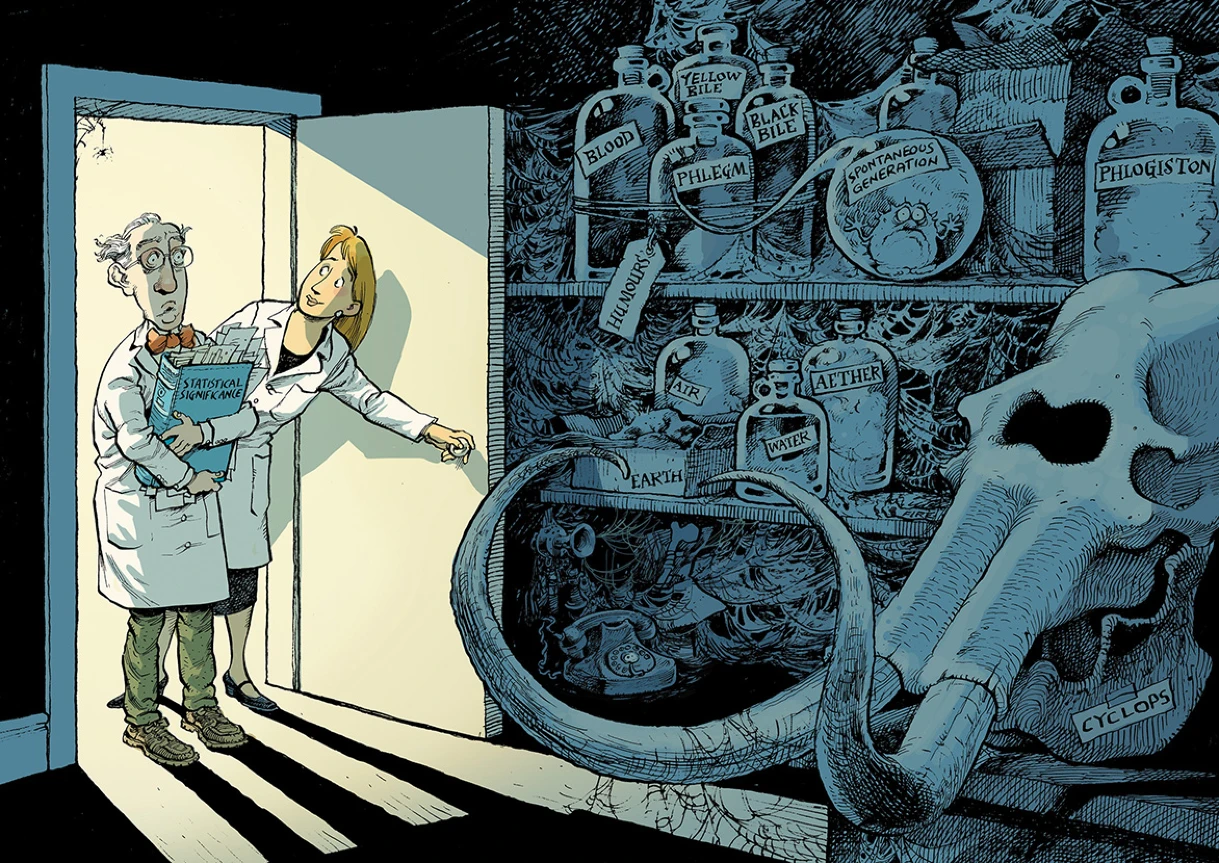
\includegraphics[width=4.06in,height=\textheight]{./www/Significance-cartoon.png}

}

\end{figure}

\hypertarget{statistical-thinking}{%
\section*{Statistical thinking}\label{statistical-thinking}}
\addcontentsline{toc}{section}{Statistical thinking}

\markright{Statistical thinking}

The work of today's data scientists is often to discover novel
connections among multiple variables and to guide decision-making. It is
common for data to be available in large masses from \emph{observations}
rather than \emph{experiments}. One common purpose is ``prediction,''
which might be as simple as the uses of medical screening tests or as
breathtaking as machine-learning techniques of ``artificial
intelligence.'' Another pressing need from data analysis is to
understand possible causal connections between variables.

The twenty lessons that follow describe a way of thinking that is
historically novel, unfamiliar to most otherwise well-educated people,
and incredibly useful for making sense of the world and what data can
tell us about the world.

\hypertarget{for-reference-important-word-pairs}{%
\section*{For reference: Important word
pairs}\label{for-reference-important-word-pairs}}
\addcontentsline{toc}{section}{For reference: Important word pairs}

\markright{For reference: Important word pairs}

Many of the vocabulary terms used in statistical thinking come in pairs.
We list several such pairs below, in roughly the order they first appear
in the Lessons. The pairs can be a reference while reading, but it is
also helpful to return to this list to sharpen your understanding of the
distinctions.

\textbf{Explanatory} vs \textbf{response} variables. Models (in these
Lessons) always involve a \emph{single} response variable*. In contrast,
models can have zero or more explanatory variables.

\textbf{Variable} vs \textbf{covariate}. ``Covariate'' is another word
for an explanatory variable. The word ``covariate'' signals that the
variable is not itself of direct interest to the modeler but puts
another explanatory variable in a correct context.

\textbf{Categorical} vs \textbf{quantitative} variables. Always be aware
of whether a model's response variable is categorical or quantitative.
When categorical, expect to use \texttt{zero\_one()} to convert it to
quantitative before modeling. In contrast, explanatory variables can be
either categorical or quantitative.

\textbf{Regression model} vs \textbf{classifier}. A regression model
always has a \emph{quantitative} response variable. A classifier has a
\emph{categorical} response variable. In these Lessons, as in much
professional use of data, our categorical response variables will have
\emph{two levels} (e.g., healthy or sick, up or down, yes or no). In
this situation, regression techniques suffice to build classifiers.

\textbf{Model} vs \textbf{model function}. By ``model,'' we will almost
always mean ``regression model.'' A regression model, typically
constructed by the \texttt{lm()} function, contains various information
useful to summarize the model. The ``model function'' provides the
mechanism for one important task, calculating from values from the
explanatory variables the corresponding model output.

\textbf{Model coefficient} vs \textbf{effect size}. Model coefficients
are numerical parameters. Training determines the appropriate values for
the coefficients. In contrast, an effect size describes the relationship
between the response variable and a selected explanatory variable.

\textbf{Point estimate} vs \textbf{interval estimate}. A point estimate
is a single number. For instance, a model coefficient is a point
estimate, as is the output from a model function. In contrast, interval
estimates involve \emph{two} numbers; one specifies the lower end of the
interval and the other number specifies the upper end.

\textbf{Prediction interval} vs \textbf{confidence interval}. A
prediction interval describes the anticipated range of the actual result
for which we have made a prediction, e.g., ``tomorrow's wind will be
between 5 and 10 mph.'' A \textbf{confidence interval} is often used to
express the uncertainty in a coefficient or effect size.

\hypertarget{software-guide}{%
\section*{Software guide}\label{software-guide}}
\addcontentsline{toc}{section}{Software guide}

\markright{Software guide}

These Lessons use about a dozen new R functions. Some of these are used
frequently in examples and exercises and are worth mastering. Others
appear only in \textbf{demonstrations}.

\begin{tcolorbox}[enhanced jigsaw, colbacktitle=quarto-callout-warning-color!10!white, breakable, opacitybacktitle=0.6, colback=white, left=2mm, arc=.35mm, colframe=quarto-callout-warning-color-frame, coltitle=black, toprule=.15mm, opacityback=0, leftrule=.75mm, bottomtitle=1mm, toptitle=1mm, titlerule=0mm, title=\textcolor{quarto-callout-warning-color}{\faExclamationTriangle}\hspace{0.5em}{Demonstrations}, rightrule=.15mm, bottomrule=.15mm]

These lessons contain \emph{demonstrations} illustrating statistical
concepts or data analysis strategies. We will place these in a
distinctive box, of which this is an example.

The demonstrations will often contain new computer commands that perform
tasks used in teaching statistics. However, readers are \textbf{not}
expected to be able to construct such commands on their own.

\end{tcolorbox}

\begin{itemize}
\tightlist
\item
  Training models with data

  \begin{itemize}
  \tightlist
  \item
    \textbf{\texttt{lm()}} arguments: i. tilde expression, ii.
    \texttt{data=} data frame.
  \item
    Occasionally, you will be directed to use \texttt{glm()} or
    \texttt{model\_train()}, which work similarly to \texttt{lm()} but
    are specialized for models whose output is a \emph{probability}.
  \item
    \textbf{\texttt{zero\_one()}} converts a two-level categorical
    variable to a 0/1 encoding.
  \end{itemize}
\item
  Summarizing models. These invariably take as input a model produced by
  \texttt{lm()} (or \texttt{glm()}) and generate a summary report about
  that model.

  \begin{itemize}
  \tightlist
  \item
    \textbf{\texttt{coef()}}: displays model coefficients. Each
    coefficient is a single number.
  \item
    \textbf{\texttt{conf\_interval()}}: displays model coefficients as
    an \emph{interval} with a lower and upper value.
  \item
    \textbf{\texttt{rsquared()}} calculates the R\textsuperscript{2} of
    a model, and some related measures.
  \item
    \textbf{\texttt{regression\_summary()}}, like
    \texttt{conf\_interval()}, but with more detail.
  \end{itemize}
\item
  Evaluating a model on inputs

  \begin{itemize}
  \tightlist
  \item
    \textbf{\texttt{model\_eval()}} takes a trained model (as produced
    by \texttt{lm()}) and calculates the model output in both a point
    form and an interval form. \texttt{model\_eval()} can also display
    the residuals from training or evaluation data.
  \end{itemize}
\item
  Graphics

  \begin{itemize}
  \tightlist
  \item
    \texttt{model\_plot()} draws a graphic of a model's function
    optionally with prediction or confidence intervals.
  \item
    \texttt{geom\_violin()} is a modern alternative to
    \texttt{geom\_boxplot()}.
  \end{itemize}
\item
  DAGs (directed, acyclic graphs)

  \begin{itemize}
  \tightlist
  \item
    \textbf{\texttt{sample()}} collects simulated data from a DAG
  \item
    \texttt{dag\_draw()} draws a picture of a DAG showing how the
    variables are connected.
  \end{itemize}
\item
  Used within the \texttt{summarize()} data wrangling function:

  \begin{itemize}
  \tightlist
  \item
    \textbf{\texttt{var()}} computes the variance of a single variable.
  \end{itemize}
\end{itemize}

\begin{tcolorbox}[enhanced jigsaw, colbacktitle=quarto-callout-warning-color!10!white, breakable, opacitybacktitle=0.6, colback=white, left=2mm, arc=.35mm, colframe=quarto-callout-warning-color-frame, coltitle=black, toprule=.15mm, opacityback=0, leftrule=.75mm, bottomtitle=1mm, toptitle=1mm, titlerule=0mm, title=\textcolor{quarto-callout-warning-color}{\faExclamationTriangle}\hspace{0.5em}{Demonstration}, rightrule=.15mm, bottomrule=.15mm]

Here are some of the command structures that appear in demonstrations.
These explanations give a general idea of the tasks they perform.

\begin{itemize}
\tightlist
\item
  \texttt{do(10)\ *\ \{} \emph{command} \texttt{\}} causes the
  \emph{command} to be executed repeatedly the indicated number of
  times. Such repetitions are useful when the \emph{command} is a trial
  of a random process such as sampling, resampling, or shuffling.
\item
  \texttt{function(}\emph{arguments}\texttt{)\ \{} \emph{set of
  commands} \texttt{\}} packages in a single unit a set of one or more
  commands. The packaging facilitates using them over and over again
  with specified arguments.
\item
  \texttt{geom\_errorbar()} works much like \texttt{geom\_point()} but
  draws vertical bars instead of dots. Bar-shaped glyphs depict
  \emph{intervals} such as confidence or prediction intervals.
\item
  \texttt{geom\_ribbon()} is like \texttt{geom\_line()} but for
  \emph{intervals}.
\item
  \texttt{effect\_size()} calculates the strength and direction of the
  input-output relationship between the response variable of a model and
  a selected \emph{one} of the explanatory variables.
\end{itemize}

\end{tcolorbox}

\part{1-18 from ModernDive}

\hypertarget{bogus}{%
\chapter{Bogus}\label{bogus}}

Foobar

\hypertarget{bogus-1}{%
\chapter{Bogus}\label{bogus-1}}

Foobar

\hypertarget{bogus-2}{%
\chapter{Bogus}\label{bogus-2}}

Foobar

\hypertarget{bogus-3}{%
\chapter{Bogus}\label{bogus-3}}

Foobar

\hypertarget{bogus-4}{%
\chapter{Bogus}\label{bogus-4}}

Foobar

\hypertarget{bogus-5}{%
\chapter{Bogus}\label{bogus-5}}

Foobar

\hypertarget{bogus-6}{%
\chapter{Bogus}\label{bogus-6}}

Foobar

\hypertarget{bogus-7}{%
\chapter{Bogus}\label{bogus-7}}

Foobar

\hypertarget{bogus-8}{%
\chapter{Bogus}\label{bogus-8}}

Foobar

\hypertarget{bogus-9}{%
\chapter{Bogus}\label{bogus-9}}

Foobar

\hypertarget{bogus-10}{%
\chapter{Bogus}\label{bogus-10}}

Foobar

\hypertarget{bogus-11}{%
\chapter{Bogus}\label{bogus-11}}

Foobar

\hypertarget{bogus-12}{%
\chapter{Bogus}\label{bogus-12}}

Foobar

\hypertarget{bogus-13}{%
\chapter{Bogus}\label{bogus-13}}

Foobar

\hypertarget{bogus-14}{%
\chapter{Bogus}\label{bogus-14}}

Foobar

\hypertarget{bogus-15}{%
\chapter{Bogus}\label{bogus-15}}

Foobar

\hypertarget{bogus-16}{%
\chapter{Bogus}\label{bogus-16}}

Foobar

\hypertarget{bogus-17}{%
\chapter{Bogus}\label{bogus-17}}

Foobar

\part{Statistical Thinking}

\hypertarget{sec-lesson-19}{%
\chapter{Preliminaries}\label{sec-lesson-19}}

\hypertarget{statistical-thinking-2}{%
\section{Statistical thinking}\label{statistical-thinking-2}}

These lessons are about ``\textbf{statistical thinking},'' a phrase
which includes habits of mind, routine questions to ask, and
understanding of which statistical measures are informative---and which
not---in different contexts. The goal of statistical thinking is to
understand ``how and when we can draw valid inferences from data.''
{[}\href{https://nobaproject.com/modules/statistical-thinking}{Source}{]}
The word ``valid'' means several things at once: faithful to the data,
consistent with the process used to assemble the data, and informative
for the uses to which the inferences are to be directed.

Every person has a natural ability to think. We train our thinking
skills by observing and emulating the logic and language of people and
sources deemed authoritative. We have resources spanning several
millennia to hone our ability to think. However, statistical thinking is
a comparatively recent arrival on the intellectual scene, germinating
and developing over only the last 150 years. As a result, hardly
anything that we hear or read exemplifies statistical thinking.

In general, effective thinking requires us to grasp various intellectual
tools, for example, logic. Our mode of logical thinking was promulgated
by Aristotle (384--322 BC) and, to quote the
\href{https://plato.stanford.edu/entries/aristotle-logic/}{Stanford
Encyclopedia of Philosophy}, ``has had an unparalleled influence on the
history of Western thought.'' In the 2500 years since Aristotle's time,
the use of Aristotelian logic has been so pervasive that we expect any
well-educated person to be able to identify logical thinking. For
example, the statement ``John's car is red'' has implications. Which of
these two statements are among those implications? ``That red car is
necessarily John's,'' or ``The blue car is not John's car.'' Not so
hard!

The intellectual tools needed for statistical thinking are, by and
large, unfamiliar and non-intuitive. These Lessons are intended to
provide the tools you will need to engage in effective statistical
thinking.

To get started, consider
\href{https://www.economist.com/international/2022/12/15/the-pandemics-indirect-effects-on-small-children-could-last-a-lifetime}{this
headline} from \emph{The Economist}, a well-reputed international news
magazine: ``The pandemic's indirect effects on small children could last
a lifetime.'' As support for this claim, the headlined article provides
more detail. For instance:

\begin{quote}
``Stress and distraction made some patients more distant. LENA, a
charity in Colorado, has for years used wearable microphones to keep
track of how much chatter babies and the care-givers exchange. During
the pandemic the number of such "conversations" declined.
\ldots.''{[}g{]}etting lots of interaction in the early years of life is
essential for healthy development, so these kinds of data "are a red
flag".'' The article goes on to talk of ``\emph{children starved of
stimulation at home \ldots.}.''
\end{quote}

This short excerpt might raise some questions. Think about it briefly
and note what questions come to mind.

For those already along the road toward statistical thinking, the
phrase, ``the number of such conversations declined'' might prompt this
question: ``By how much?'' Similarly, reading the claim that ``getting
lots of interactions \ldots{} is essential for healthy development,''
your mind might insist on these questions: How much is ``lots?'' How
does the decline in the number compare to ``lots?''

Not finding the answer to these questions in the article's text, it
would be sensible to look for the primary source of the information. In
our Internet age, that's comparatively easy to do. The LENA website
includes
\href{https://www.lena.org/covid-infant-vocalizations-conversational-turns/}{an
article}, ``COVID-era infants vocalize less and experience fewer
conversational turns, says LENA research team.'' The article contains
two graphs. (\textbf{?@fig-lena-two-graphs})

\begin{Shaded}
\begin{Highlighting}[]
\NormalTok{knitr}\SpecialCharTok{::}\FunctionTok{include\_graphics}\NormalTok{(}\StringTok{"www/Lena{-}fig1.png"}\NormalTok{)}
\NormalTok{knitr}\SpecialCharTok{::}\FunctionTok{include\_graphics}\NormalTok{(}\StringTok{"www/Lena{-}fig2.png"}\NormalTok{)}
\end{Highlighting}
\end{Shaded}

\begin{figure}

\begin{minipage}[t]{0.50\linewidth}

{\centering 

\raisebox{-\height}{

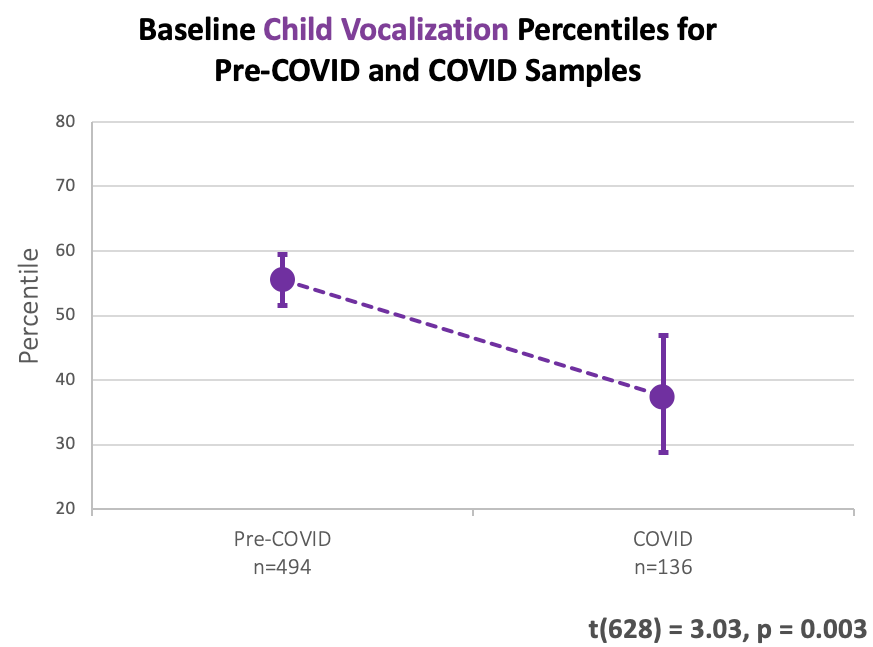
\includegraphics[width=2.91in,height=\textheight]{./www/Lena-fig1.png}

}

\caption{\label{fig-lena-two-graphs-1}Graphics from the LENA website.
The left is captioned, ``Children from the COVID-era sample produced
significantly fewer vocalizations than their pre-COVID peers.'' The
right, ``The differences in vocalizations and turns were greatest among
children from families in the lowest SES {[}socio-economic status{]}
quartile.''}

}

\end{minipage}%
%
\begin{minipage}[t]{0.50\linewidth}

{\centering 

\raisebox{-\height}{

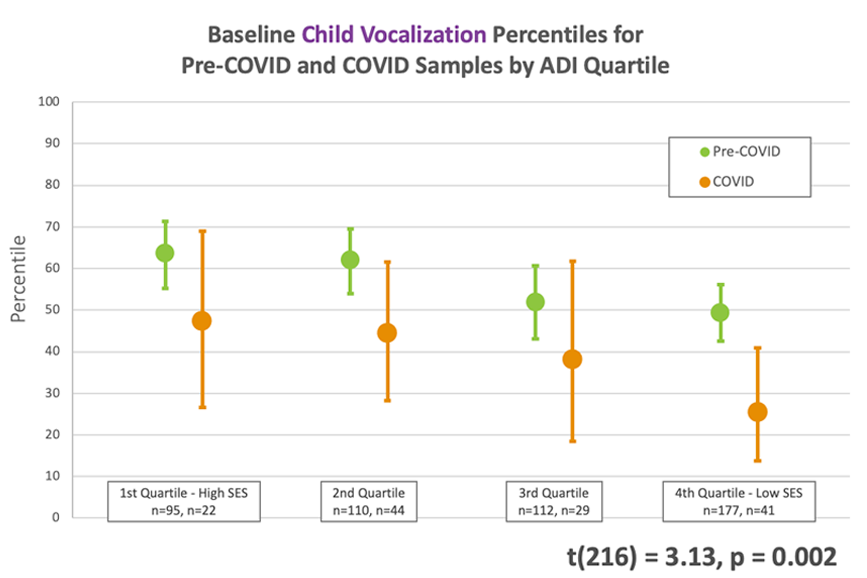
\includegraphics[width=2.89in,height=\textheight]{./www/Lena-fig2.png}

}

\caption{\label{fig-lena-two-graphs-2}Graphics from the LENA website.
The left is captioned, ``Children from the COVID-era sample produced
significantly fewer vocalizations than their pre-COVID peers.'' The
right, ``The differences in vocalizations and turns were greatest among
children from families in the lowest SES {[}socio-economic status{]}
quartile.''}

}

\end{minipage}%

\end{figure}

To make any proper sense of the graphs in
\textbf{?@fig-lena-two-graphs}, you need some basic technical knowledge.
For example, what do the vertical bars in the graph mean? And the
subcaptions, ``t(628) = 3.03, p = 0.003'' and ``t(216)= 2.13, p=0.002'':
What do they mean, if anything? Turning back to the text of \emph{The
Economist}, do these graphs justify raising a ``red flag?'' More
basically, are these graphs the ``data,'' or is there more data behind
the graphs? What would that data show?

The LENA article does not link to supporting data, that is, what lies
behind the graphs in \textbf{?@fig-lena-two-graphs}. But the LENA
article does point to other publications.

\begin{quote}
``\emph{These findings from LENA support a growing body of evidence that
babies born during the COVID pandemic are, on average, experiencing
developmental delays. For example, researchers from the COMBO (COVID-19
Mother Baby Outcomes) consortium at Columbia University published
findings in the
\href{www/jamapediatrics_shuffrey_2022_oi_210081_1653493590.2509.pdf}{January
2022 issue of JAMA Pediatrics} showing that children born during the
pandemic achieved significantly lower gross motor, fine motor, and
personal-social scores at six months of age.}''
\end{quote}

To the statistical thinker, phrases like ``red flag,'' ``growing body of
evidence,'' and ``significantly lower'' are \textbf{weasel words}, that
is, terms ``used in order to evade or retreat from a direct or
forthright statement or position.''
{[}\href{https://www.merriam-webster.com/dictionary/weasel\%20word}{Source}{]}
In ordinary thinking, such evasiveness or lack of forthrightness would
naturally prompt concern about the reliability of the claim. It makes
sense to look deeper, for instance, by checking out the JAMA article.
Many people would be hesitant to do this, anticipating that the article
would be incomprehensible and filled with jargon. An important reason to
study statistical thinking is to tear down barriers to substantiating or
debunking claims. In fact, the JAMA article contains very little that
requires knowledge of pediatrics or the meaning of ``gross motor, fine
motor, and personal-social scores,'' but a lot that depends on
understanding statistical notation and convention and---more critical
---the reasoning behind the conventions.

The tools of statistical thinking are the tools for making sense of
data. Evaluating data is essential to determine whether to rely on
claims supposedly based on those data. In the words of eminent engineer
and statistician
\href{https://en.wikipedia.org/wiki/W._Edwards_Deming}{W. Edwards
Demming}: ``In God we trust. All others must bring data.'' And former
President Ronald Reagan famously quoted a Russian proverb: ``Trust, but
verify.'' Unfortunately, until you have the statistical thinking tools
needed to interpret data reliably, all you can do is trust, not verify.

\hypertarget{defining-statistical-thinking}{%
\section{Defining statistical
thinking}\label{defining-statistical-thinking}}

Learning a new way of thinking is genuinely hard. As you learn
statistical thinking, it may help to have a concise definition. The
following definition captures much of the essence of statistical
thinking:

\begin{quote}
\emph{Statistic thinking is the accounting for variation} in the context
of \emph{what remains unaccounted for.}
\end{quote}

Implicit in this definition is a pathway for learning to think
statistically:

\begin{enumerate}
\def\labelenumi{\arabic{enumi}.}
\tightlist
\item
  Learn how to measure variation;
\item
  Learn how to account for variation;
\item
  Learn how to measure what remains unaccounted for.
\end{enumerate}

The next three sections briefly touch on each of these three topics.

\hypertarget{variation}{%
\section{Variation}\label{variation}}

\begin{figure*}

\begin{quote}
\emph{Variation itself is nature's only irreducible essence. Variation
is the hard reality, not a set of imperfect measures for a central
tendency. Means and medians are the abstractions.} ----- Stephen Jay
Gould (1941- 2002), paleontologist and historian of science.
\end{quote}

\end{figure*}

To illustrate variation, let's consider a process fundamental to human
life: gestation. We all know that human pregnancy ``typically'' lasts
around nine-months, but that the duration isn't known in advance.

Figure~\ref{fig-gestation-jitter} shows data from the \texttt{Gestation}
data frame. In this data frame, each of the 1200 rows is one pregnancy
and birth about which several measurements were made. The
\texttt{gestation} variable records the length of the pregnancy (in
days).

\begin{Shaded}
\begin{Highlighting}[]
\NormalTok{Gestation }\OtherTok{\textless{}{-}}\NormalTok{ Gestation }\SpecialCharTok{\%\textgreater{}\%} 
  \FunctionTok{mutate}\NormalTok{(}\AttributeTok{parity =} \FunctionTok{ifelse}\NormalTok{(parity}\SpecialCharTok{==}\DecValTok{0}\NormalTok{, }\StringTok{"first{-}time"}\NormalTok{, }\StringTok{"previous{-}preg"}\NormalTok{)) }
\NormalTok{Plot1 }\OtherTok{\textless{}{-}}\NormalTok{ Gestation }\SpecialCharTok{\%\textgreater{}\%}
  \FunctionTok{ggplot}\NormalTok{(}\FunctionTok{aes}\NormalTok{(}\AttributeTok{x=}\NormalTok{parity, }\AttributeTok{y=}\NormalTok{gestation)) }\SpecialCharTok{+} 
  \FunctionTok{geom\_jitter}\NormalTok{(}\AttributeTok{alpha=}\FloatTok{0.2}\NormalTok{, }\AttributeTok{width=}\FloatTok{0.2}\NormalTok{, }\AttributeTok{height=}\DecValTok{0}\NormalTok{) }
\NormalTok{Plot1}
\end{Highlighting}
\end{Shaded}

\begin{figure}[H]

\sidecaption{\label{fig-gestation-jitter}Gestational period for
first-time mothers and mothers with a previous pregancy.}

{\centering 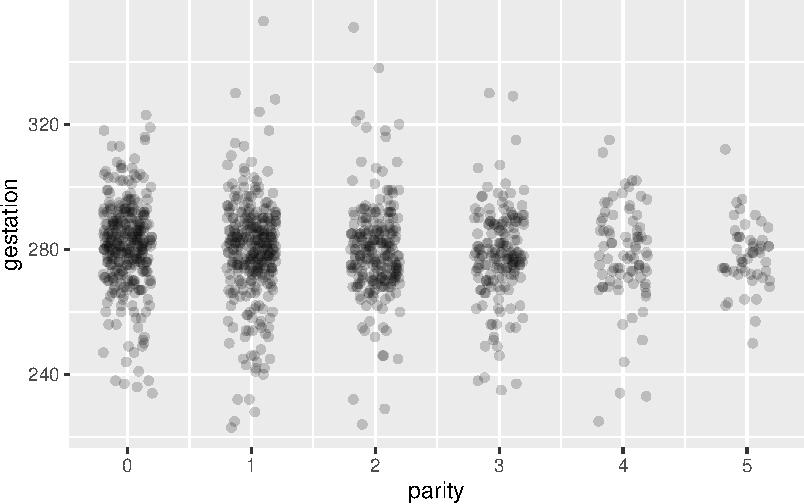
\includegraphics{./Reading-notes-lesson-19_files/figure-pdf/fig-gestation-jitter-1.pdf}

}

\end{figure}

Figure~\ref{fig-gestation-jitter} divides the 1200 births in the
\texttt{Gestation} data frame according to the variable \texttt{parity},
which describes whether or not the pregnancy is the mother's first.

The variation in \texttt{gestation} is evident directly from the dots in
the graph. One strategy for describing variation is to specify an
\textbf{interval}: the span between a lower and an upper value. For
instance,

\begin{itemize}
\tightlist
\item
  The large majority of pregancies last between 250 and 300 days. Or,
\item
  The majority of pregnancies are between 275 and 290 days.
\end{itemize}

A more subtle description avoids setting hard bounds in favor of saying
which durations are common and which not. This common-or-not description
is called a ``\textbf{distribution}.'' The ``\textbf{histogram}'' is a
famous style of presentation of a distribution. Even elementary-school
students are introduced to histograms; they are easy to draw. But we
have more important concerns; we want to be able to show relationships
between variables and we want, whenever possible, to put the graphical
summaries of data as a layer on top of the data themselves. And we have
the computer as a tool for making graphics. Consequently, our preferred
format for displaying distributions is a smooth shape, oriented along
the vertical axis. The width of the shape expresses how common is the
corresponding region of the vertical axis. Figure~\ref{fig-violin-intro}
shows the density display layered on top of the pregnancy data. For
reasons that may be evident, this sort of display is called a
``\textbf{violin plot}.''

\begin{Shaded}
\begin{Highlighting}[]
\NormalTok{Plot1 }\SpecialCharTok{+}
  \FunctionTok{geom\_violin}\NormalTok{(}\FunctionTok{aes}\NormalTok{(}\AttributeTok{group=}\NormalTok{parity), }\AttributeTok{fill=}\StringTok{"blue"}\NormalTok{, }\AttributeTok{alpha=}\FloatTok{0.65}\NormalTok{, }\AttributeTok{color=}\ConstantTok{NA}\NormalTok{)}
\end{Highlighting}
\end{Shaded}

\begin{figure}[H]

\sidecaption{\label{fig-violin-intro}A violin plot. The long axis of the
violin-like shape is oriented along the response-variable axis (that is,
the vertical axis in our standard format). The width of the violin for
each possible value of the response variable is proportional to the
density of data near that value.}

{\centering 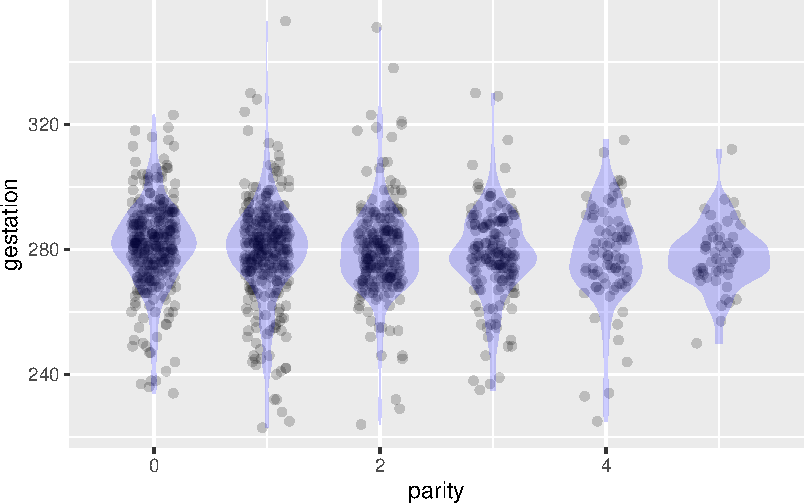
\includegraphics{./Reading-notes-lesson-19_files/figure-pdf/fig-violin-intro-1.pdf}

}

\end{figure}

The shapes of the two violins in Figure~\ref{fig-violin-intro} are
similar, suggesting that the variation in the duration of pregnancy is
about the same for first-time mothers as for mothers in a second or
later pregnancy.

There is a strong link between the \emph{interval} descriptions of
variation and the density display. Suppose you specify the fraction of
cases that you want to include in an interval description, say 50\% or
80\%. In terms of the violin, that fraction is a proportion of the
overall \textbf{area} of the violin. For instance, the 50\% interval
would include the central 50\% of the area of the violin, leaving 25\%
out at the bottom and another 25\% out at the top. The 80\% interval
would leave out only 10\% of the area at the top and bottom of the
violin. This suggests that the interval style of describing variation
really involves \emph{three} numbers; the top and bottom of the interval
\emph{as well as} the selected percentage (say, 50\% or 80\%) used to
find the location of the top and bottom.

Yet another style for describing variation---one that will take primary
place in these Lessons---uses only a \textbf{single-number}. Perhaps the
simplest way to imagine how a \emph{single} number can capture variation
is to think about the \emph{spread} or \emph{distance} between the top
and bottom of an interval description. In taking such a distance as the
measure of variation, we are throwing out some information. Taken
together, the top and bottom of the interval describe two things: the
\emph{location} of the values and the \emph{spread} among the values.
These are both important, but it is the \emph{spread} that gives a pure
description of variation.

Early pioneers of statistics took some time to agree on a standard way
of measuring the spread. For instance, should it be the spread between
the top and bottom of a 50\% interval or an 80\% interval, or something
else. In the end, the selected standard focussed on something more
basic: the differences between pairs of individual values.

It works like this. For a data frame with \(n=2\) rows, the spread in a
variable can be measured simply as the \emph{difference} between the two
values. For instance, suppose the \texttt{gestation} variable had only
two entries, say, 267 and 293 days. The spread or distance between these
is \(293-267 = 26\) days. Of course, we don't intend to measure spread
with a negative number. One solution is to use the absolute value of the
difference. However, for subtle mathematical reasons relating to---of
all things!---the Pythagorean theorem, we avoid the possibility of a
negative spread by using the \emph{square of the difference}, that is,
\((293 - 267)^2 = 676\) days-squared.

To extend this very simple measure of variation to data with \(n > 2\)
is simple: look at the square difference between every possible pair of
values, then average. For instance, for \(n=3\) with values 267, 293,
284, look at the differences \((267-293)^2, (267-284)^2\) and
\((293-284)^2\) and average them! This simple way of measuring variation
is called the ``modulus'' and dates from 1885. Since then, statisticians
have standardized on a closely related measure, the
``\textbf{variance},'' which is the modulus divided by \(\sqrt{2}\).
Either one would work, but there are advantages to standardizing on one:
the variance.

Calculating the variance is straightforward, Here's the variance of
\texttt{gestation}:

\begin{Shaded}
\begin{Highlighting}[]
\NormalTok{Gestation }\SpecialCharTok{\%\textgreater{}\%}
  \FunctionTok{summarize}\NormalTok{(}\AttributeTok{variance =} \FunctionTok{var}\NormalTok{(gestation))}
\end{Highlighting}
\end{Shaded}

\ttfamily 
\begin{tabular}{r}
\toprule
variance\\
\midrule
256.887\\
\bottomrule
\end{tabular} \normalfont
\bigskip

A consequence of the use of squaring in defining the variance is the
units of the result. \texttt{gestation} is measured in days, so
\texttt{var(gestation)} is measured in days\textsuperscript{2}. The
advantage to this will only become clear later in these Lessons. For
now, you might prefer to think about the square-root of the variance,
which has been given the name ``\textbf{standard deviation}.''

\begin{Shaded}
\begin{Highlighting}[]
\NormalTok{Gestation }\SpecialCharTok{\%\textgreater{}\%}
  \FunctionTok{summarize}\NormalTok{(}\AttributeTok{standard\_deviation =} \FunctionTok{sd}\NormalTok{(gestation))}
\end{Highlighting}
\end{Shaded}

\ttfamily 
\begin{tabular}{r}
\toprule
standard\_deviation\\
\midrule
16.02769\\
\bottomrule
\end{tabular} \normalfont
\bigskip

\hypertarget{sec-accounting-for-variation}{%
\section{Accounting for variation}\label{sec-accounting-for-variation}}

The word ``account'' has several related meanings.\footnote{These are
  drawn from the Oxford Languages dictionaries.}

\begin{itemize}
\tightlist
\item
  To ``account for something'' means ``to be the explanation or cause of
  something.'' {[}Oxford Languages{]}
\item
  An ``account of something'' is a story, a description, or an
  explanation, as in the Biblical account of the creation of the world.
\item
  To ``take account of something'' means ``to consider particular facts,
  circumstances, etc. when making a decision about something.''
\end{itemize}

Synonyms for ``account'' include ``description,''report,'' ``version,''
``story,'' ``statement,'' ``explanation,'' ``interpretation,''
``sketch,'' and ``portrayal.'' ``Accountants'' and their ``account
books'' keep track of where money comes from and goes to.

These various nuances of meaning, from a simple arithmetical tallying up
to an interpretation or version serve the purposes of statistical
thinking well. When we ``account for variation,'' we are telling a story
that tries to explain where the variation might have come from. An
accounting of variation is not necessarily definitive, true, or helpful.
Just as witnesses of an event can have different accounts, so there can
be many accounts of the variation even of the same variable in the same
data frame.

There are many formats for stories, many ways of organizing facts and
data, and many ways of accounting for variance. In these Lessons, we
will use \textbf{regression modeling} almost exclusively as our method
of accounting. Here, for example, are two different accounts of
\texttt{gestation}:

\begin{Shaded}
\begin{Highlighting}[]
\FunctionTok{lm}\NormalTok{(gestation }\SpecialCharTok{\textasciitilde{}} \DecValTok{1}\NormalTok{, }\AttributeTok{data=}\NormalTok{Gestation) }\SpecialCharTok{\%\textgreater{}\%} \FunctionTok{coef}\NormalTok{()}
\end{Highlighting}
\end{Shaded}

\begin{verbatim}
(Intercept) 
   279.3385 
\end{verbatim}

\begin{Shaded}
\begin{Highlighting}[]
\FunctionTok{lm}\NormalTok{(gestation }\SpecialCharTok{\textasciitilde{}}\NormalTok{ parity, }\AttributeTok{data =}\NormalTok{ Gestation) }\SpecialCharTok{\%\textgreater{}\%} \FunctionTok{coef}\NormalTok{()}
\end{Highlighting}
\end{Shaded}

\begin{verbatim}
        (Intercept) parityprevious-preg 
         281.261981           -2.585058 
\end{verbatim}

In the R language, expressions like
\texttt{gestation\ \textasciitilde{}\ 1} and
\texttt{gestation\ \textasciitilde{}\ parity} are called ``tilde
expressions.'' They are the means by which the modeler
\textbf{specifies} the structure of the model that is to be built.
Training (or ``fitting'') translates the \textbf{model specification}
into an arithmetic formula that involves the explanatory variables and
numerical coefficients.

The coefficients from a regression model are part of an accounting for
variation. Learning how to read them is an important skill in
statistical thinking. For instance, the coefficient from a model in the
form \texttt{y\ \textasciitilde{}\ 1} is always the average value of
variable \texttt{y}. In contrast, in a model like
\texttt{y\ \textasciitilde{}\ x}, the ``intercept'' is a baseline value
and the \texttt{x}-coefficient describes what part of the variation in
\texttt{y} can be credited to \texttt{x}.

\begin{tcolorbox}[enhanced jigsaw, colbacktitle=quarto-callout-note-color!10!white, breakable, opacitybacktitle=0.6, colback=white, left=2mm, arc=.35mm, colframe=quarto-callout-note-color-frame, coltitle=black, toprule=.15mm, opacityback=0, leftrule=.75mm, bottomtitle=1mm, toptitle=1mm, titlerule=0mm, title=\textcolor{quarto-callout-note-color}{\faInfo}\hspace{0.5em}{The RESPEX graphics format}, rightrule=.15mm, bottomrule=.15mm]

Figure~\ref{fig-gestation-jitter} is an example of what we call the
\textbf{RESPEX} graphics style. Each RESPEX graphic is made to
coordinate with aregression model of the data. Every regression model
has a response variable. Likewise, every RESPEX graphic shows the
response variable on the vertical axis. Similarly, RESPEX graphics place
an explanatory variable on the horizontal axis. If there is more than
one explanatory variable, they are encoded graphically using color then
faceting.

RESPEX stands for ``RESPonse versus EXplanatory,'' but you might like to
think of it as data graphics drawn with ``respect'' to a model.

\end{tcolorbox}

Regression models always have a quantitative response variable, although
explanatory variables can be either quantitative or categorical. But,
often, the modeling situation calls for a response variable that is
\emph{categorical}. Expert modelers can use specialized modeling methods
to handle such situations. However, some of the power of these
specialized methods is available to the beginning modeler by a little
trick. When categorical response variables have just two levels, e.g.,
Alive/Dead, Promoted/Not, or Win/Loss, they can be transformed to a
numerical representation using 0 for one level and 1 for the other.

We will identify the such variables as being of type ``\textbf{yes/no}''
or, equivalently, ``\textbf{zero-one}'' variables. With the zero-one
encoding

This numerical ``\textbf{0/1 encoding}'' is directly suited for
regression modeling and enables us to extend the scope of regression
models. The \emph{output} of the regression model is always numerical.
Nothing in the regression technique restricts those outputs to exactly
zero or one, even when the response variable is of the yes/no type.
Usually, the modeler interprets such numerical output as probabilities
or, more generally, as measures to be converted to probabilities.

\begin{tcolorbox}[enhanced jigsaw, colbacktitle=quarto-callout-note-color!10!white, breakable, opacitybacktitle=0.6, colback=white, left=2mm, arc=.35mm, colframe=quarto-callout-note-color-frame, coltitle=black, toprule=.15mm, opacityback=0, leftrule=.75mm, bottomtitle=1mm, toptitle=1mm, titlerule=0mm, title=\textcolor{quarto-callout-note-color}{\faInfo}\hspace{0.5em}{R technique: \texttt{zero\_one()}.}, rightrule=.15mm, bottomrule=.15mm]

The \texttt{zero\_one()} function converts a yes/no variable to the
numerical zero-one format. \texttt{zero\_one()} allows you to specify
which of the two levels is represented by 1.

To illustrate, consider the \texttt{mosaicData::Whickham} data frame,
which records a 1972-1974 survey, part of a study of the relationship
between smoking and mortality. Twenty years after the initial survey, a
follow-up established whether or not each person was still alive. Here
are a few rows from the data frame:

\ttfamily 
\begin{tabular}{llr}
\toprule
outcome & smoker & age\\
\midrule
Alive & Yes & 23\\
Alive & Yes & 18\\
Dead & Yes & 71\\
Alive & No & 67\\
Alive & No & 64\\
\addlinespace
Alive & Yes & 38\\
\bottomrule
\end{tabular} \normalfont
\bigskip

The \texttt{outcome} variable in \texttt{Whickham} records the result of
the follow-up survey. It is a categorical variable with levels ``Alive''
and ``Dead.'' To examine what the data have to say about the
relationship between smoking and mortality, we construct a model with
\texttt{outcome} as the response variable and \texttt{smoking} as an
explanatory variable. Before doing so, we translate \texttt{outcome}
into a zero-one format. Like this:

\begin{Shaded}
\begin{Highlighting}[]
\NormalTok{Whickham }\SpecialCharTok{\%\textgreater{}\%} 
  \FunctionTok{mutate}\NormalTok{(}\AttributeTok{alive =} \FunctionTok{zero\_one}\NormalTok{(outcome, }\AttributeTok{one=}\StringTok{"Alive"}\NormalTok{))}
\end{Highlighting}
\end{Shaded}

\ttfamily 
\begin{tabular}{llrr}
\toprule
outcome & smoker & age & alive\\
\midrule
Alive & Yes & 23 & 1\\
Alive & Yes & 18 & 1\\
Dead & Yes & 71 & 0\\
Alive & No & 67 & 1\\
Alive & No & 64 & 1\\
\addlinespace
Alive & Yes & 38 & 1\\
\bottomrule
\end{tabular} \normalfont
\bigskip

Note the correspondence between the \texttt{outcome} and the newly
created \texttt{alive} variable.

\end{tcolorbox}

\hypertarget{variation-unaccounted-for}{%
\section{Variation unaccounted for}\label{variation-unaccounted-for}}

A model typically accounts for only some of the variation in a response
variable. The remaining variation is called ``\textbf{residual
variation}.''

Consider the model \texttt{gestation\ \textasciitilde{}\ parity}. In the
next lines of code we build this model, training it with the
\texttt{Gestation} data. Then we \textbf{evaluate} the model on the
trained data. This amounts to using the model coefficients to generate a
model output for each row in the training data, and can be accomplished
with the \texttt{model\_eval()} R function.

\begin{Shaded}
\begin{Highlighting}[]
\NormalTok{Model }\OtherTok{\textless{}{-}} \FunctionTok{lm}\NormalTok{(gestation }\SpecialCharTok{\textasciitilde{}}\NormalTok{ parity, }\AttributeTok{data =}\NormalTok{ Gestation)}
\NormalTok{Evaluated }\OtherTok{\textless{}{-}} \FunctionTok{model\_eval}\NormalTok{(Model)}
\end{Highlighting}
\end{Shaded}

\begin{verbatim}
Using training data as input to model_eval().
\end{verbatim}

\begin{verbatim}
Using training data as input to model_eval().
\end{verbatim}

\ttfamily 
\begin{tabular}{lrlrrrr}
\toprule
  & .response & parity & .output & .resid & .lwr & .upr\\
\midrule
1218 & 270 & previous-preg & 278.6769 & -8.6769231 & 247.2800 & 310.0738\\
1219 & 275 & first-time & 281.2620 & -6.2619808 & 249.8322 & 312.6917\\
1220 & 265 & previous-preg & 278.6769 & -13.6769231 & 247.2800 & 310.0738\\
1221 & 291 & previous-preg & 278.6769 & 12.3230769 & 247.2800 & 310.0738\\
1222 & 281 & first-time & 281.2620 & -0.2619808 & 249.8322 & 312.6917\\
\addlinespace
1223 & 297 & previous-preg & 278.6769 & 18.3230769 & 247.2800 & 310.0738\\
\bottomrule
\end{tabular} \normalfont
\bigskip

\begin{tcolorbox}[enhanced jigsaw, colbacktitle=quarto-callout-note-color!10!white, breakable, opacitybacktitle=0.6, colback=white, left=2mm, arc=.35mm, colframe=quarto-callout-note-color-frame, coltitle=black, toprule=.15mm, opacityback=0, leftrule=.75mm, bottomtitle=1mm, toptitle=1mm, titlerule=0mm, title=\textcolor{quarto-callout-note-color}{\faInfo}\hspace{0.5em}{The \texttt{.response} variable}, rightrule=.15mm, bottomrule=.15mm]

The output from \texttt{model\_eval()} repeats some columns from the
data used for evaluation. For example, the explanatory variables are
listed by name. (Here, the only explanatory variable is
\texttt{parity}.) The response variable is also included, but given a
generic name, \texttt{.response} to make it easy to distinguish it from
the explanatory variables.

\end{tcolorbox}

To see where the \texttt{.output} comes from, let's look again at the
model coefficients:

\begin{Shaded}
\begin{Highlighting}[]
\NormalTok{Model }\SpecialCharTok{\%\textgreater{}\%} \FunctionTok{coef}\NormalTok{()}
\end{Highlighting}
\end{Shaded}

\begin{verbatim}
        (Intercept) parityprevious-preg 
         281.261981           -2.585058 
\end{verbatim}

The baseline value is 281.3 days. This applies to first-time mothers.
For the other mothers, those with a previous pregnancy, the coefficient
indicates that the model value is 2.6 days \emph{less} than the
baseline, or 279.7 days.

The output from \texttt{model\_eval()} includes other columns of
importance. For us, here, those are. the response variable itself
(\texttt{gestation}, which has been given a generic name,
\texttt{.response}) and the residuals from the model (\texttt{.resid}).
There is a simple relationship between \texttt{.response},
\texttt{.output} and \texttt{.resid}:

\[\mathtt{.response} = \mathtt{.output} + \mathtt{.resid}\]

\begin{tcolorbox}[enhanced jigsaw, colbacktitle=quarto-callout-warning-color!10!white, breakable, opacitybacktitle=0.6, colback=white, left=2mm, arc=.35mm, colframe=quarto-callout-warning-color-frame, coltitle=black, toprule=.15mm, opacityback=0, leftrule=.75mm, bottomtitle=1mm, toptitle=1mm, titlerule=0mm, title=\textcolor{quarto-callout-warning-color}{\faExclamationTriangle}\hspace{0.5em}{Demonstration: Why the variance?}, rightrule=.15mm, bottomrule=.15mm]

The subtle mathematical reasoning behind the choice of \emph{variance}
to measure variation is illuminated when we compute the variances of the
three quantities in the previous equation.

\begin{Shaded}
\begin{Highlighting}[]
\NormalTok{Evaluated }\SpecialCharTok{\%\textgreater{}\%}
  \FunctionTok{summarize}\NormalTok{(}\AttributeTok{var\_response =} \FunctionTok{var}\NormalTok{(.response),}
            \AttributeTok{var\_output =} \FunctionTok{var}\NormalTok{(.output),}
            \AttributeTok{var\_resid  =} \FunctionTok{var}\NormalTok{(.resid))}
\end{Highlighting}
\end{Shaded}

\ttfamily 
\begin{tabular}{rrr}
\toprule
var\_response & var\_output & var\_resid\\
\midrule
256.887 & 1.273587 & 255.6134\\
\bottomrule
\end{tabular} \normalfont
\bigskip

The variances of the output and residuals add up to equal, exactly, the
variance of the response variable! This isn't true for the standard
deviations:

\begin{Shaded}
\begin{Highlighting}[]
\NormalTok{Evaluated }\SpecialCharTok{\%\textgreater{}\%}
  \FunctionTok{summarize}\NormalTok{(}\AttributeTok{sd\_response =} \FunctionTok{sd}\NormalTok{(.response),}
            \AttributeTok{sd\_output =} \FunctionTok{sd}\NormalTok{(.output),}
            \AttributeTok{sd\_resid  =} \FunctionTok{sd}\NormalTok{(.resid))}
\end{Highlighting}
\end{Shaded}

\ttfamily 
\begin{tabular}{rrr}
\toprule
sd\_response & sd\_output & sd\_resid\\
\midrule
16.02769 & 1.128533 & 15.98791\\
\bottomrule
\end{tabular} \normalfont
\bigskip

\end{tcolorbox}

\hypertarget{sec-lesson-20}{%
\chapter{Simulation and sampling variation}\label{sec-lesson-20}}

Carl Wieman is a Nobel-prize-winning physicist and professor of
education at Stanford University. Weiman
\href{https://ed.stanford.edu/about/community/carl-wieman}{writes},
``For many years, I had two parallel research programs: one blasting
atoms with lasers to see how they'd behave, and another studying how
people learn.'' Some of Wieman's work on learning deals with the nature
of ``\textbf{expertise}.'' He points out that experts have
\href{https://www.youtube.com/watch?v=12oJzN5I4H8}{ways to monitor their
own thinking and learning}; they have a body of knowledge relevant to
checking their own understanding.

This lesson presents you with two tools: simulation and repetition.
Simulation enables you to generate variation with known properties,
where you know the sources of variation and how variables are connected.
Then you can experiment to find out how to use statistical models to
reveal the underlying properties.

The second tool, repetition, helps you deal with randomness and quantify
precision. By repeating the same simulation many times while introducing
basic random fluctuations, you can figure out the extent to which
randomness can be tamed.

\hypertarget{directed-acyclic-graphs}{%
\section{Directed Acyclic Graphs}\label{directed-acyclic-graphs}}

A core tool in thinking about causal connections is a mathematical
structure called a ``directed acyclic graph'' (DAG, for short). DAGs are
one of the most popular ways for statistical thinkers to express their
ideas about what might be happening in the real world. Despite the long
name, DAGs are very accessible to a broad audience.

DAGs, despite the G for ``graph,'' are not about data graphics. The
``graph'' in DAG is a mathematical term of art; a suitable synonym is
``network.'' Mathematical graphs consist of a set of ``nodes'' and a set
of ``edges'' connecting the nodes. For instance, Figure~\ref{fig-graphs}
shows three different graphs, each with five nodes labeled A, B, C, D,
and E.

\begin{figure*}

\begin{minipage}[t]{0.33\linewidth}

{\centering 

\raisebox{-\height}{

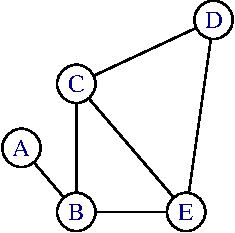
\includegraphics{./Reading-notes-lesson-20_files/figure-pdf/fig-graphs-1.pdf}

}

}

\subcaption{\label{fig-graphs-1}undirected graph}
\end{minipage}%
%
\begin{minipage}[t]{0.33\linewidth}

{\centering 

\raisebox{-\height}{

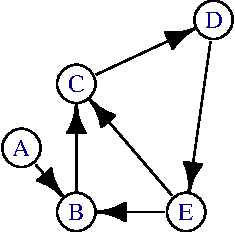
\includegraphics{./Reading-notes-lesson-20_files/figure-pdf/fig-graphs-2.pdf}

}

}

\subcaption{\label{fig-graphs-2}directed but cyclic}
\end{minipage}%
%
\begin{minipage}[t]{0.33\linewidth}

{\centering 

\raisebox{-\height}{

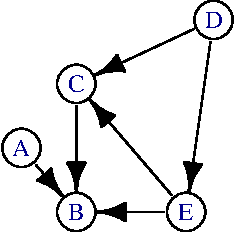
\includegraphics{./Reading-notes-lesson-20_files/figure-pdf/fig-graphs-3.pdf}

}

}

\subcaption{\label{fig-graphs-3}directed acyclic graph}
\end{minipage}%

\caption{\label{fig-graphs}Graphs of various types}

\end{figure*}

The nodes are the same in all three graphs of Figure~\ref{fig-graphs},
but each graph is different from the others. It is not just the nodes
that define a graph; the edges (drawn as lines) are part of the
definition as well.

The left-most graph in Figure~\ref{fig-graphs} is an
``\textbf{undirected}'' graph; there is no suggestion that the edges run
one way or another. In contrast, the middle graph has the same nodes and
edges, but the edges are \textbf{directed}. An excellent way to think
about a directed graph is that each node is a pool of water; each
directed edge shows how the water flows between pools. This analogy is
also helpful in thinking about causality: the causal influences flow
like water.

Look more carefully at the middle graph. There is a couple of loops; the
graph is \textbf{cyclic}. In one loop, water flows from E to C to D and
back again to E. The other loop runs B, C, D, E, and back to B. Such a
flow pattern cannot exist without pumps pushing the water back uphill.

The rightmost graph reverses the direction of some of the edges. This
graph has no cycles; it is \textbf{acyclic}. Using the flowing and
pumped water analogy, an acyclic graph needs no pumps; the pools can be
arranged at different heights to create a flow exclusively powered by
gravity. The node-D pool will be the highest, E lower. C has to be lower
than E for gravity to pull water along the edge from E to C. The node-B
pool is the lowest, so water can flow in from E, C, and A.

Directed acyclic graphs represent causal influences; think of ``A causes
B,'' meaning that causal ``water'' flows naturally from A to B. In a
DAG, a node can have multiple outputs, like D and E, and it might have
multiple inputs, like B and C. In terms of causality, a node---like
B---having multiple inputs means that more than one factor is
responsible for the value of that node. A real-world example: the rising
sun causes a rooster to crow, but so can another intruder to the coop.

Often, nodes do not have any inputs. These are called
``\textbf{exogenous factors}''at least by economists. The ``genous''
means ``originates from.'' ``Exo'' means ``outside.'' The value of an
exogenous node is determined by something, just not something that we
are interested in (or perhaps capable of) modeling. No edges are
directed into an exogenous node since none of the other nodes influence
its value.

For simulating data, we go beyond drawing a graph of causal connections
to outfit DAGs with specific formulas representing the mechanism imbued
in each node. DAGs equipped with formulas can be used to generate
simulated data.\footnote{The value of exogenous nodes is usually set
  randomly, without input from the other nodes in the DAG.} Training a
model on those data leads to a model function that we can compare to the
DAG's formulas. Then check whether the formulas and the model function
match. This practice helps us learn what can go right or wrong in
building a model, just as practice in an aircraft simulator trains
pilots to handle real-world situations in real aircraft.

We start with a simple example, \texttt{dag08}. The \texttt{dag\_draw()}
command draws a picture of the graph. Printing the dag displays the
formulas that set the values of the nodes.

\begin{Shaded}
\begin{Highlighting}[]
\FunctionTok{dag\_draw}\NormalTok{(dag08)}
\end{Highlighting}
\end{Shaded}

\begin{figure}[H]

{\centering 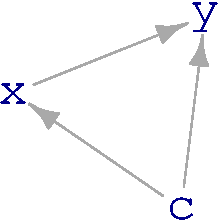
\includegraphics{./Reading-notes-lesson-20_files/figure-pdf/unnamed-chunk-3-1.pdf}

}

\end{figure}

The graph shows that both \texttt{c} and \texttt{x} contribute to
\texttt{y}.

\begin{Shaded}
\begin{Highlighting}[]
\FunctionTok{print}\NormalTok{(dag08)}
\end{Highlighting}
\end{Shaded}

\begin{verbatim}
c ~ exo()
x ~ c + exo()
y ~ x + c + 3 + exo()
\end{verbatim}

The formulas show that \texttt{x} and \texttt{c} contribute equally to
\texttt{y}, with coefficients of 1. To what extent can regression
modeling recover this relationship from data?

To find out, we can generate simulated data using the \texttt{sample()}
function. For instance,

\begin{Shaded}
\begin{Highlighting}[]
\FunctionTok{sample}\NormalTok{(dag08, }\AttributeTok{size=}\DecValTok{5}\NormalTok{)}
\end{Highlighting}
\end{Shaded}

\ttfamily 
\begin{tabular}{rrr}
\toprule
c & x & y\\
\midrule
-0.3260365 & 0.8479298 & 4.048341\\
0.5524619 & 1.1712517 & 3.928869\\
-0.6749438 & -0.7876782 & 2.965133\\
0.2143595 & 1.1313877 & 2.878928\\
0.3107692 & 0.0875099 & 3.161596\\
\bottomrule
\end{tabular} \normalfont
\bigskip

Each row in the sample is one trial; in each trial, the node's formula
sets the value for that node. For example, the formula might use the
values of other nodes as input. Alternatively, the formula might specify
that the node is exogenous, without input from any other nodes.

Models can be trained on the simulated data using the same techniques as
for any other data. To illustrate, here we generate a sample of size
\(n=50\), then fit the model specification
\texttt{c\ \textasciitilde{}\ a\ +\ b} and summarize by taking the
coefficients.

\begin{Shaded}
\begin{Highlighting}[]
\FunctionTok{sample}\NormalTok{(dag08, }\AttributeTok{size=}\DecValTok{50}\NormalTok{) }\SpecialCharTok{\%\textgreater{}\%} 
  \FunctionTok{lm}\NormalTok{(y }\SpecialCharTok{\textasciitilde{}}\NormalTok{ c }\SpecialCharTok{+}\NormalTok{ x, }\AttributeTok{data =}\NormalTok{ .) }\SpecialCharTok{\%\textgreater{}\%}
  \FunctionTok{coef}\NormalTok{()}
\end{Highlighting}
\end{Shaded}

\begin{verbatim}
(Intercept)           c           x 
  2.9451445   1.2606473   0.8235923 
\end{verbatim}

The coefficients, including the intercept, are close, but not exactly
right.

In Lessons -Chapter~\ref{sec-lesson-21} and -Chapter~\ref{sec-lesson-22}
we will figure out how close we can expect the coefficients to be to the
precise values implemented in the simulation.

\hypertarget{samples-summaries-of-samples-and-samples-of-summaries-of-samples}{%
\section{Samples, summaries of samples, and samples of summaries (of
samples)}\label{samples-summaries-of-samples-and-samples-of-summaries-of-samples}}

Beginners sometimes think that each row in a data frame is a sample.
Better to say that each row is a ``\textbf{specimen}.'' A
``\textbf{sample}'' is a collection of specimens, the set of rows in a
data frame.

The ``\textbf{sample size}'' is the number of rows.
``\textbf{Sampling}'' is the process of collecting the specimens to be
put into the data frame.

The following command illustrates computing a summary of a sample from
\texttt{dag08}.

\begin{Shaded}
\begin{Highlighting}[]
\FunctionTok{sample}\NormalTok{(dag08, }\AttributeTok{size=}\DecValTok{10000}\NormalTok{) }\SpecialCharTok{\%\textgreater{}\%} 
  \FunctionTok{lm}\NormalTok{(y }\SpecialCharTok{\textasciitilde{}}\NormalTok{ c }\SpecialCharTok{+}\NormalTok{ x, }\AttributeTok{data =}\NormalTok{ .) }\SpecialCharTok{\%\textgreater{}\%}
  \FunctionTok{coef}\NormalTok{()}
\end{Highlighting}
\end{Shaded}

\begin{verbatim}
(Intercept)           c           x 
  3.0070253   1.0100177   0.9934592 
\end{verbatim}

An essential question in statistics is how the summary depends on the
incidental specifics of a particular sample. DAGs provide a convenient
way to address this question since we can generate multiple samples from
the same DAG, summarize each, and compare those summaries.

To generate a sample of summaries, re-run many trials of the summary.
The \texttt{do()} function automates this process, accumulating the
results from the trials in a single data frame: a ``\textbf{sample of
summaries}.'' We will use \texttt{do()} mostly in demonstrations.

\begin{tcolorbox}[enhanced jigsaw, colbacktitle=quarto-callout-warning-color!10!white, breakable, opacitybacktitle=0.6, colback=white, left=2mm, arc=.35mm, colframe=quarto-callout-warning-color-frame, coltitle=black, toprule=.15mm, opacityback=0, leftrule=.75mm, bottomtitle=1mm, toptitle=1mm, titlerule=0mm, title=\textcolor{quarto-callout-warning-color}{\faExclamationTriangle}\hspace{0.5em}{Demonstration: Conducting many trials with \texttt{do()}}, rightrule=.15mm, bottomrule=.15mm]

In this demonstration, we will revisit a model used earlier in this
Lesson to see how much the coefficients vary from one sample to another.
Each trial consists of drawing a sample from \texttt{dag08}, training a
model, and summarizing with the model coefficients. Curly braces
(\texttt{\{} and \texttt{\}}) surround the commands needed for an
individual trial.

Preceding the curly braces, we have placed \texttt{do(5)\ *}. This
instruction causes the trial to be repeated five times.

\begin{Shaded}
\begin{Highlighting}[]
\FunctionTok{do}\NormalTok{(}\DecValTok{5}\NormalTok{) }\SpecialCharTok{*}\NormalTok{ \{}
  \FunctionTok{sample}\NormalTok{(dag08, }\AttributeTok{size=}\DecValTok{50}\NormalTok{) }\SpecialCharTok{\%\textgreater{}\%} 
    \FunctionTok{lm}\NormalTok{(y }\SpecialCharTok{\textasciitilde{}}\NormalTok{ c }\SpecialCharTok{+}\NormalTok{ x, }\AttributeTok{data =}\NormalTok{ .) }\SpecialCharTok{\%\textgreater{}\%}
    \FunctionTok{coef}\NormalTok{()}
\NormalTok{\}}
\end{Highlighting}
\end{Shaded}

\ttfamily 
\begin{tabular}{rrr}
\toprule
Intercept & c & x\\
\midrule
3.019112 & 0.6794641 & 1.3353393\\
3.006728 & 0.9042066 & 0.8406397\\
2.966061 & 1.1619847 & 0.9307029\\
2.866499 & 1.0881640 & 1.0769612\\
3.080889 & 1.1088753 & 1.0009938\\
\bottomrule
\end{tabular} \normalfont
\bigskip

The five trials are collected together by \texttt{do()} into the five
rows of a single data frame. Such a data frame can be considered a
``\textbf{sample of summaries}.''

\end{tcolorbox}

One of the things we will do with a ``sample of summaries'' is to
\ldots{} wait for it \ldots{} summarize it. For instance, in the
following code chunk, a sample of 40 summaries is stored under the name
\texttt{Trials}. Then we will summarize \texttt{Trials}, in this case,
to see how much the values of the \texttt{a} and \texttt{b} coefficients
vary from trial to trial.

\begin{Shaded}
\begin{Highlighting}[]
\NormalTok{Trials }\OtherTok{\textless{}{-}} \FunctionTok{do}\NormalTok{(}\DecValTok{40}\NormalTok{) }\SpecialCharTok{*}\NormalTok{ \{}
  \FunctionTok{sample}\NormalTok{(dag08, }\AttributeTok{size=}\DecValTok{50}\NormalTok{) }\SpecialCharTok{\%\textgreater{}\%} 
    \FunctionTok{glm}\NormalTok{(y }\SpecialCharTok{\textasciitilde{}}\NormalTok{ c }\SpecialCharTok{+}\NormalTok{ x, }\AttributeTok{data =}\NormalTok{ .) }\SpecialCharTok{\%\textgreater{}\%}
    \FunctionTok{coef}\NormalTok{()}
\NormalTok{\} }
\NormalTok{Trials }\SpecialCharTok{\%\textgreater{}\%} 
  \FunctionTok{summarize}\NormalTok{(}\AttributeTok{mean\_c\_coef =} \FunctionTok{mean}\NormalTok{(c), }\AttributeTok{spread\_a =} \FunctionTok{sd}\NormalTok{(c), }
            \AttributeTok{mean\_x\_coef =} \FunctionTok{mean}\NormalTok{(x), }\AttributeTok{spread\_b =} \FunctionTok{sd}\NormalTok{(c))}
\end{Highlighting}
\end{Shaded}

\ttfamily 
\begin{tabular}{rrrr}
\toprule
mean\_c\_coef & spread\_a & mean\_x\_coef & spread\_b\\
\midrule
0.9858736 & 0.2215985 & 1.022228 & 0.2215985\\
\bottomrule
\end{tabular} \normalfont
\bigskip

The result of summarizing the trials is a ``summary of a sample of
summaries.'' This phrase is admittedly awkward, but we will use this
technique often: summarizing trials, where each trial is a ``summary of
a sample'' Often, the clue will be the use of \texttt{do()}, which
repeats trials as many times as you ask.

\hypertarget{causal-inference}{%
\section{Causal inference}\label{causal-inference}}

Often, but not always, our interest in studying data is to reveal or
exploit the causal connections between variables. Understanding
causality is essential, for instance, if we are planning to intervene in
the world and want to anticipate the consequences. Interventions are
things like ``increase the dose of medicine,'' ``stop smoking!'',
``lower the budget,'' ``add more cargo to a plane (which will increase
fuel consumption and reduce the range).''

Historically, mainstream statisticians were hostile to using data to
explore causal relationships. (The one exception was
\textbf{experiment}, which gathers data from an actual intervention in
the world. See Lesson~\ref{sec-lesson-32}.) Statistics teachers
encouraged students to use phrases like ``associated with'' or
``correlated with'' and reminded them that ``correlation is not
causation.''

Regrettably, this attitude made statistics irrelevant to the many
situations where intervention is the core concern and experiment was not
feasible. A tragic episode of this sort likely caused millions of
unnecessary deaths. Starting in the 1940s, doctors and epidemiologists
saw evidence that smoking causes lung cancer. In stepped the most famous
statistician of the age, Ronald Fisher, to insist that the statement
should be, ``smoking is associated with lung cancer.'' He speculated
that smoking and lung cancer might have a common cause, perhaps genetic.
Fisher argued that establishing causation requires running an experiment
where people are randomly assigned to smoke or not smoke and then
observed for decades to see if they developed lung cancer. Such an
experiment is unfeasible and unethical, to say nothing of the need to
wait decades to get a result.

Fortunately, around 1960, a researcher at the US National Institutes of
Health, Jerome Cornfield, was able to show mathematically that the
strength of the association between smoking and cancer ruled out any
genetic mechanism. Cornfield's work was an important step in the
development of a new area in statistics: ``\textbf{causal inference}.''

Causal inference is not about proving that one thing causes another but
about formal ways to say something about how the world works that can be
used, along with data, to make responsible conclusions about causal
relationships.

As you will see in Lesson -Chapter~\ref{sec-lesson-30}, DAGs are a major
tools in causal inference, allowing you not only to represent a
hypothesis about causal relationships, but to deduce what sorts of
models will be able to reveal causal mechanisms.

The point of a DAG is to make a clear statement of a hypothesis about
causation. Drawing a DAG does not mean that the hypothesis is correct,
just that we believe the hypothesis is, in some sense, a possibility.
Different people might have different beliefs about what causes what in
real-world systems. Comparing their different DAGs can help, sometimes,
to discuss and resolve the disagreement.

We are going to use DAGs for two distinct purposes. One purpose is to
inform responsible conclusions from data about what causes what. The
data on its own is insufficient to demonstrate the causal connections.
However, data \emph{combined with} a DAG can tell us something.
Sometimes a DAG includes a causal connection that should create an
association between variables. The DAG is incomplete if the association
does not appear in the data.

DAGs are also valuable aids for building models. For example, analysis
of the paths in a DAG, as in Lesson~\ref{sec-lesson-30}, can tell us
which explanatory variables to include and which to exclude from a model
if our modeling goal is to represent the hypothetical causal
connections.

In these Lessons, we have a second, entirely different, use for DAGs:
learning modeling technique. Our approach will be to :::
\{.callout-warning\} \#\# Reality check: DAGs and data

DAGs represent hypotheses about the connections between variables in the
real world. They are a kind of scratchpad for constructing alternative
scenarios and, as seen in Lesson~\ref{sec-lesson-28}, thinking about how
models might go wrong in the face of a plausible alternative causal
mechanism.

In this book, we extend the use of DAGs beyond their scope in
professional statistics; we use them as simulations from which we can
generate data. Such simulations provide one way to learn about
statistical methodology.

DAGs are aides to reasoning, scratchpads that help us play out the
consequences of our hypotheses about possible real-world mechanisms.
However, take caution to distinguish data from DAG simulations from data
from reality.

Finding out about the real world requires collecting data from the real
world. The proper role of DAGs in real work is to guide model building
\textbf{from real data}.

In this course, we sample from DAGs to learn statistical techniques. But
never to make claims about real-world phenomena. :::

\hypertarget{sec-lesson-21}{%
\chapter{Signal and noise}\label{sec-lesson-21}}

Imagine being transported back to June 1940. The family is in the living
room, sitting around the radio console, waiting for it to warm up. The
news today is from Europe, the surrender of the French in the face of
the German invasion. Press the play button and listen to recording
\#103.

{\marginnote{\begin{footnotesize}You may have to scroll down to see the
play button and the recordings.\end{footnotesize}}}

The spoken words from the recording are discernible despite the hiss and
clicks of the background noise. The situation is similar to a
conversation in a sports stadium. The crowd is loud, so the speaker has
to shout. The listener ignores the noise (unless it is too loud) and
recovers the shouted words.

Engineers and others make a distinction between \textbf{signal} and
noise. The engineer aims to separate the signal from the noise. That aim
applies to statistics as well.

There are many sources of noise in data; every variable has its own
story, part of which is noise from measurement errors and recording
blunders. For instance, economists use national statistics, like GDP,
even though the definition is arbitrary (a Hurricane can raise GDP!),
and early reports are invariably corrected a few months later.
Historians go back to original documents, but inevitably many of the
documents have been lost or destroyed: a source of noise. Even in
elections where, in principle, counting is straightforward, the voters'
intentions are measured imperfectly due to ``hanging chads,''
``butterfly ballots,'' broken voting machines, spoiled ballots, and so
on.

The statistical thinker is well advised to know about the sources of
noise in the system she is studying. Analysis of data will be better the
more the modeler knows about how measurements are made and data
collected.

\begin{tcolorbox}[enhanced jigsaw, colbacktitle=quarto-callout-note-color!10!white, breakable, opacitybacktitle=0.6, colback=white, left=2mm, arc=.35mm, colframe=quarto-callout-note-color-frame, coltitle=black, toprule=.15mm, opacityback=0, leftrule=.75mm, bottomtitle=1mm, toptitle=1mm, titlerule=0mm, title=\textcolor{quarto-callout-note-color}{\faInfo}\hspace{0.5em}{Noise in hiring}, rightrule=.15mm, bottomrule=.15mm]

The author has, on several occasions, testified in legal hearings as a
statistical expert. In one case, the US Department of Labor audited the
records of a contractor with several hundred employees and high employee
turnover. The records led the Department to bring suit against the
contractor for discriminating against Hispanics. The hiring records
showed that many Hispanics applied for jobs; the company hired none. An
open-and-shut case.

The lawyers for the defense asked me, the statistical expert, to review
the findings from the Department of Labor. The lawyers thought they were
asking me to check the arithmetic in the hiring spreadsheets. As a
statistical thinker, I know that arithmetic is only part of the story;
the origin of the data is critically important. So I asked for the
complete files on all applicants and hires the previous year.

The spreadsheet files and the paper job applications were in accord;
there were many Hispanic applicants. But the data on the paper job
application form was not always consistent with the data on hiring
spreadsheets. It turned out that whenever an applicant was hired, the
contractor (per regulation) got a report on that person from the state
police. The report returned by the state police had only two available
race/ethnicities: white and Black. The contractor's personnel office
filled in the hired-worker spreadsheet based on the state police report.
So all the Hispanic applicants who were hired had been transformed into
white or Black by the state police. Noise.

\end{tcolorbox}

\hypertarget{sec-signal-and-noise}{%
\section{Signal and noise}\label{sec-signal-and-noise}}

To illustrate the statistical problem of signal and noise, let us turn
to a DAG simulation: \texttt{dag01}. Here's a sample from
\texttt{dag01}:

\begin{Shaded}
\begin{Highlighting}[]
\NormalTok{Tiny }\OtherTok{\textless{}{-}} \FunctionTok{sample}\NormalTok{(dag01, }\AttributeTok{size=}\DecValTok{2}\NormalTok{)}
\end{Highlighting}
\end{Shaded}

\ttfamily 
\begin{tabular}{rr}
\toprule
x & y\\
\midrule
-0.3260365 & 2.836001\\
0.5524619 & 5.043052\\
\bottomrule
\end{tabular} \normalfont
\bigskip

The DAG simulation implements a relationship between \texttt{x} and
\texttt{y}. In statistics, this \emph{relationship} is the signal.

\begin{quote}
Look at the 2-row sample (\textbf{?@tbl-tiny-dag01}) from the DAG and
guess what the relationship might be.
\end{quote}

Any of an infinite number of possible relationships could account for
the \texttt{x} and \texttt{y} data. The noise reduction problem of
statistics is to make a guess that is as good as possible.
Unfortunately, for a sample with \(n=2\), as ``good as possible'' is not
very good!

More data---a bigger sample---gives us a better shot at revealing the
relationship hidden by the noise. \textbf{?@tbl-small-dag01} shows a
sample of size \(n=10\):

\begin{Shaded}
\begin{Highlighting}[]
\NormalTok{Small }\OtherTok{\textless{}{-}} \FunctionTok{sample}\NormalTok{(dag01, }\AttributeTok{size=}\DecValTok{10}\NormalTok{)}
\end{Highlighting}
\end{Shaded}

\ttfamily 
\begin{tabular}{rr}
\toprule
x & y\\
\midrule
-0.7859732 & 1.8888204\\
0.0547389 & 4.1153256\\
-1.1725603 & 2.3632792\\
-0.1673128 & 6.3287614\\
-1.8650316 & 0.9329524\\
\addlinespace
-0.1204402 & 2.9310384\\
0.8259787 & 5.6981878\\
1.1901595 & 5.9006170\\
-1.0914519 & 2.1314570\\
-0.3751124 & 4.2296648\\
\bottomrule
\end{tabular} \normalfont
\bigskip

A careful perusal of the \texttt{Small} sample suggests some patterns.
\texttt{x} is never larger than about 2 in magnitude and can be positive
or negative. \texttt{y} is always positive. Furthermore, when \texttt{x}
is negative, the corresponding \texttt{y} value is relatively small
compared to the \texttt{y} values for positive \texttt{x}.

A sample of size \(n=10\) provides more information than a sample of
\(n=2\), so we can make a more informed guess about the relationship
between variables \texttt{x} and \texttt{y}.

Human cognition is not well suited to looking at long columns of
numbers. Often, we can make better use of our natural human talents by
translating the sample into a graphic:

\includegraphics{./Reading-notes-lesson-21_files/figure-pdf/unnamed-chunk-6-1.pdf}

Collecting more data can make the relationship clearer.
Figure~\ref{fig-xy-relationship-large} displays an \(n=10,000\) sample.

\begin{Shaded}
\begin{Highlighting}[]
\NormalTok{Large }\OtherTok{\textless{}{-}} \FunctionTok{sample}\NormalTok{(dag01, }\AttributeTok{size=}\DecValTok{10000}\NormalTok{)}
\end{Highlighting}
\end{Shaded}

\begin{figure}

\sidecaption{\label{fig-xy-relationship-large}With \(n=10,000\) rows,
the relationship between \texttt{x} and \texttt{y} is evident
graphically. (The original \texttt{Small} sample is shown in orange.)}

{\centering 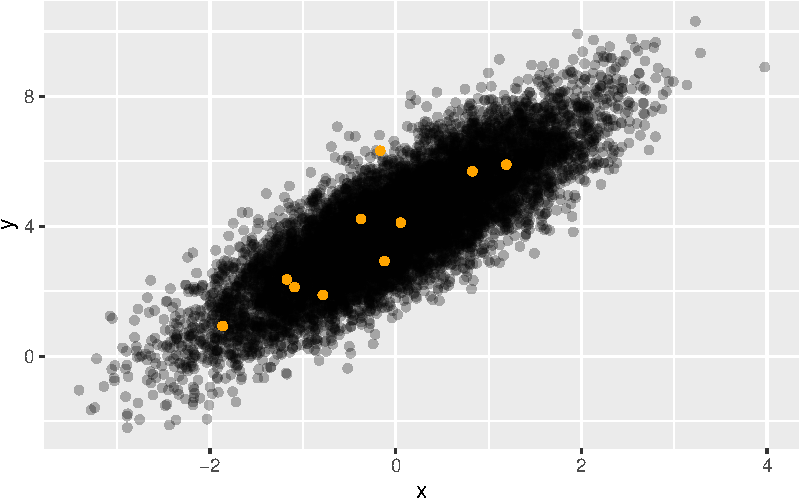
\includegraphics{./Reading-notes-lesson-21_files/figure-pdf/fig-xy-relationship-large-1.pdf}

}

\end{figure}

There are many possible ways to describe the x-y relationship in
Figure~\ref{fig-xy-relationship-large}. For instance, we can see that
when \texttt{x} is positive, \texttt{y} is almost always greater than 4,
but for negative \texttt{x}, the value of \texttt{y} tends to be less
than 4. Such a description might be apt for some purposes, but in these
Lessons, we describe relationships by fitting models to data.

The following command uses the small sample (n=10) as training data for
a model \texttt{y\ \textasciitilde{}\ x} that accounts for \texttt{y} on
the basis of \texttt{x}:

\begin{Shaded}
\begin{Highlighting}[]
\FunctionTok{lm}\NormalTok{(y }\SpecialCharTok{\textasciitilde{}}\NormalTok{ x, }\AttributeTok{data =}\NormalTok{ Small) }\SpecialCharTok{\%\textgreater{}\%} \FunctionTok{coef}\NormalTok{()  }\CommentTok{\# n = 10 sample}
\end{Highlighting}
\end{Shaded}

\begin{verbatim}
(Intercept)           x 
   4.262846    1.741758 
\end{verbatim}

The coefficients provide the information needed to construct the
\emph{model function}: \[y = 4.26 + 1.74 x\ .\] This mathematical
formula is a guess of the \emph{signal}---the relationship between the
two variables in \texttt{dag01}. Unfortunately, the formula tells us
nothing about the noise obscuring the signal nor how good the guess is.

The model coefficients produced by training the model on a much larger
sample will presumably be a better guess:

\begin{Shaded}
\begin{Highlighting}[]
\FunctionTok{lm}\NormalTok{(y }\SpecialCharTok{\textasciitilde{}}\NormalTok{ x, }\AttributeTok{data =}\NormalTok{ Large) }\SpecialCharTok{\%\textgreater{}\%} \FunctionTok{coef}\NormalTok{() }\CommentTok{\#  n = 10,000 sample}
\end{Highlighting}
\end{Shaded}

\begin{verbatim}
(Intercept)           x 
   4.008928    1.495904 
\end{verbatim}

Unfortunately, we cannot tell from the coefficients how good the guess
is.

Luckily for us, since the data are a simulation from a DAG, we can see
what the coefficients \emph{should be} as well as the origin of the
noise mixing in with the signal.

\begin{Shaded}
\begin{Highlighting}[]
\FunctionTok{print}\NormalTok{(dag01)}
\end{Highlighting}
\end{Shaded}

\begin{verbatim}
x ~ exo()
y ~ 1.5 * x + 4 + exo()
\end{verbatim}

The \texttt{Large} sample produced coefficients much closer than the
\texttt{Small} sample to the mechanism in the DAG. The idea that larger
samples lead to better accuracy has been appreciated since the 16th
century and now has the prestige of being a ``Law'': the Law of Large
Numbers.

However, ``better accuracy'' does not tell us whether the accuracy
suffices for any given purpose. The model filters out some of the noise.
However, the model coefficients still display a noisy legacy.

The challenge of real-world data is that we cannot open the black box
that generated the data; all we have is the data! So how can we tell
whether the data at hand are sufficient for giving a usefully accurate
description of the actual relationships?

The key to the puzzle is the variation \emph{within} the sample.

\hypertarget{measuring-variation}{%
\section{Measuring variation}\label{measuring-variation}}

Lesson~\ref{sec-lesson-19} introduced the standard way to measure
variation in a single variable: the \textbf{variance} or its square
root, the \textbf{standard deviation}. For instance, we can measure the
variation in the variables from the \texttt{Large} sample using
\texttt{sd()} and \texttt{var()}:

\begin{Shaded}
\begin{Highlighting}[]
\NormalTok{Large }\SpecialCharTok{\%\textgreater{}\%}
  \FunctionTok{summarize}\NormalTok{(}\AttributeTok{sx =} \FunctionTok{sd}\NormalTok{(x), }\AttributeTok{sy =} \FunctionTok{sd}\NormalTok{(y), }\AttributeTok{vx =} \FunctionTok{var}\NormalTok{(x), }\AttributeTok{vy =} \FunctionTok{var}\NormalTok{(y))}
\end{Highlighting}
\end{Shaded}

\ttfamily 
\begin{tabular}{rrrr}
\toprule
sx & sy & vx & vy\\
\midrule
0.9830639 & 1.779003 & 0.9664146 & 3.164851\\
\bottomrule
\end{tabular} \normalfont
\bigskip

According to the standard deviation, the size of the \texttt{x}
variation is about 1. The size of the \texttt{y} variation is about 1.7.

Look again at the formulas that compose \texttt{dag01}:

\begin{Shaded}
\begin{Highlighting}[]
\FunctionTok{print}\NormalTok{(dag01)}
\end{Highlighting}
\end{Shaded}

\begin{verbatim}
x ~ exo()
y ~ 1.5 * x + 4 + exo()
\end{verbatim}

The formula for \texttt{x} shows that \texttt{x} is endogenous, its
values coming from a random number generator, \texttt{exo()}, which,
unless otherwise specified, generates noise of size 1.

As for \texttt{y}, the formula includes two sources of variation:

\begin{enumerate}
\def\labelenumi{\arabic{enumi}.}
\tightlist
\item
  The part of \texttt{y} determined by \texttt{x}, that is
  \(y = \mathbf{1.5 x} + \color{gray}{4 + \text{exo()}}\)
\item
  The noise added directly into \texttt{y}, that is
  \(y = \color{gray}{\mathbf{1.5 x} + 4} + \color{black}{\mathbf{exo(\,)}}\)
\end{enumerate}

The 4 in the formula does not add any \emph{variation} to \texttt{y}; it
is just a number.

We already know that \texttt{exo()} generates random noise of size 1. So
the amount of variation contributed by the \texttt{+\ exo()} term in the
DAG formula is 1. The remaining variation is contributed by
\texttt{1.5\ *\ x}. The variation in \texttt{x} is 1 (coming from the
\texttt{exo()} in the formula for \texttt{x}). A reasonable guess is
that \texttt{1.5\ *\ x} will have 1.5 times the variation in \texttt{x}.
So, the variation contributed by the \texttt{1.5\ *\ x} component is
1.5. The overall variation in \texttt{y} is the sum of the variations
contributed by the individual components. This suggests that the
variation in \texttt{y} should be
\[\underbrace{1}_\text{from exo()} + \underbrace{1.5}_\text{from 1.5 x} = \underbrace{2.5}_\text{overall variation in y}.\]
Simple addition! Unfortunately, the result is wrong. In the previous
summary of the \texttt{Large}, we measured the overall variation in
\texttt{y} as about 1.72.

The \emph{variance} will give a better accounting than the standard
deviation. Recall that \texttt{exo()} generates variation whose standard
deviation is 1, so the variance from \texttt{exo()} is \(1^2 = 1\).
Since \texttt{x} comes entirely from \texttt{exo()}, the variance of
\texttt{x} is 1. So is the variance of the \texttt{exo()} component of
\texttt{y}.

Turn to the \texttt{1.5\ *\ x} component of \texttt{y}. Since variances
involve squares, the variance of \texttt{1.5\ *\ x} works out to be
\(1.5^2\, \text{var(}\mathit{x}\text{)} = 2.25\). Adding up the
variances from the two components of \texttt{y} gives

\[\text{var(}\mathit{y}\text{)} = \underbrace{2.25}_\text{from 1.5 exo()} + \underbrace{1}_\text{from exo()} = 3.25\]

This result that the variance of \texttt{y} is 3.25 closely matches what
we found in summarizing the \texttt{y} data generated by the DAG.

\textbf{The lesson here}: When adding two sources of variation, the
variances of the individual sources add to form the overall variance of
the sum. Just like \(A^2 + B^2 = C^2\) in the Pythagorean Theorem.

\hypertarget{dags-from-data}{%
\section{DAGs from data}\label{dags-from-data}}

In modeling data from \texttt{dag01} we could recover a good
approximation to the formula for \texttt{y}.

\begin{Shaded}
\begin{Highlighting}[]
\NormalTok{Large }\SpecialCharTok{\%\textgreater{}\%}
  \FunctionTok{lm}\NormalTok{(y }\SpecialCharTok{\textasciitilde{}}\NormalTok{ x, }\AttributeTok{data =}\NormalTok{ .) }\SpecialCharTok{\%\textgreater{}\%}
  \FunctionTok{coef}\NormalTok{()}
\end{Highlighting}
\end{Shaded}

\begin{verbatim}
(Intercept)           x 
   4.008928    1.495904 
\end{verbatim}

A DAG describes the causal links between variables. Data modeling
reveals the formula implementing the causal link in \texttt{dag01}.
Nevertheless, it is wrong to think we can determine the DAG that
generated the data from the data alone. Only if we already know the
structure of the data-generation DAG can we recover the mechanism inside
that DAG. For instance, another statistical thinker might believe that
the causal mechanism behind the data is \texttt{y} causing \texttt{x}.
Based on this assumption, she also can find the mechanism inside her
hypothesized DAG:

\begin{Shaded}
\begin{Highlighting}[]
\FunctionTok{sample}\NormalTok{(dag01, }\AttributeTok{size=}\DecValTok{10000}\NormalTok{) }\SpecialCharTok{\%\textgreater{}\%}
  \FunctionTok{lm}\NormalTok{(x }\SpecialCharTok{\textasciitilde{}}\NormalTok{ y, }\AttributeTok{data =}\NormalTok{ .) }\SpecialCharTok{\%\textgreater{}\%}
  \FunctionTok{coef}\NormalTok{()}
\end{Highlighting}
\end{Shaded}

\begin{verbatim}
(Intercept)           y 
 -1.8261448   0.4559782 
\end{verbatim}

A DAG is a \textbf{hypothesis}, a statement that might or might not be
true. DAGs are part of the statistical apparatus for thinking
responsibly about \textbf{causality}. Use a DAG---or, potentially,
multiple DAGs---when the issue of what causes what is relevant to the
purpose behind the work.

When there are only two variables involved in the system under
consideration---we will call them X and Y for simplicity---there are
only two possible DAGs:

\[X \rightarrow Y\ \ \ \ \ \text{and}\ \ \ \ \ X \leftarrow Y\] Our
understanding of the world sometimes allows us to focus on one of these
and not the other. Example: Does the rooster crowing cause the sun to
rise, or does the rising sun cause the rooster to crow?

Beyond the two DAGs \(X \rightarrow Y\) and \(X \leftarrow Y\),
additional DAG possibilities can account for the relationship between X
and Y. For instance, if we introduce another variable, C, located
between X and Y, four other DAGs need to be considered:

\[X \rightarrow C \rightarrow Y \ \ \ \ \ \text{and}\ \ \ \ \
X \leftarrow C \leftarrow Y \ \ \ \ \ \text{and}\ \ \ \ \
X \leftarrow C \rightarrow Y \ \ \ \ \ \text{and}\ \ \ \ \
X \rightarrow C \leftarrow Y\]

There are many other DAG configurations involving three variables. To
keep things simple, we will restrict things to DAGs where X might or
might not cause Y, but Y never causes X.\footnote{We do not lose
  generality by this restriction. The modeler gets to choose which
  real-world variable corresponds to X and which one to Y.}
Figure~\ref{fig-ten-triples} shows the ten configurations of 3-variable
DAGs where Y does not cause X.

\begin{figure}

\sidecaption{\label{fig-ten-triples}Ten DAG configurations involving
three variables X, Y, and C.}

{\centering 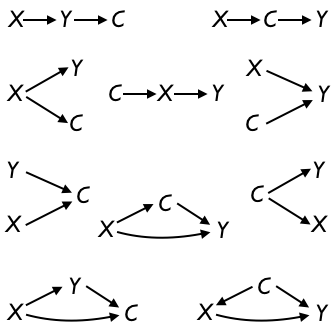
\includegraphics[width=1.2\textwidth,height=\textheight]{./www/ten-triples.png}

}

\end{figure}

With the conceptual tool of DAGs, the statistical thinker can consider
multiple possibilities for what might cause what. Sometimes she can
discard some of the possibilities based on common sense. (Think:
roosters and the sun.) However, in other settings, there may be
possibilities that she does not favor but might be plausible to other
people. In Lesson~\ref{sec-lesson-28}, we will explore how each
configuration of DAG has implications for which model specifications can
or cannot reveal the hypothesized causal mechanism.

\hypertarget{sec-lesson-22}{%
\chapter{Sampling and sampling variation}\label{sec-lesson-22}}

\textbf{Sampling variation} is a subtle concept. Part of the difficulty
in understanding sampling variation is the meaning of the word
``sample,'' which differs in use between everyday speech and statistical
language. In everyday speech, a sample is:

\begin{quote}
``\emph{A small part or quantity intended to show what the whole is
like.}'' --- Oxford Languages
\end{quote}

A food market will give you a sample of an item on sale: a tiny cup of a
drink or a taste of a piece of fruit or other food item.
Laundry-detergent companies sometimes send out a sample of their product
in the form of a small foil packet suitable for only a single wash
cycle. Paint stores keep small samples on hand to help customers choose
from among the possibilities. A fabric sample is a little swatch of
cloth cut from a a bigger bolt that a customer is considering buying.

In contrast, a \textbf{sample} in statistics is always a
\emph{collection} of multiple items. Usually, a sample is presented to
us in the form of a data frame which records the measured attributes of
each of the items in the sample. While it is possible for a data frame
to have just a single row, it is perverse to use the word ``sample'' to
describe a single item. Instead, we use other words to point to a single
item: for instance ``a case,'' ``a row,'' ``an individual,'' ``a
datum,'' or ``a specimen.'' Samples, like the word ``data,'' are always
plural. Think of ``sample'' as akin to words like ``herd,'' ``flock'',
``pack'', or ``school'': a collective. A single fish is not a school and
a single wolf is not a pack. Similarly, a single row is not a sample but
an item.

The dictionary definition of ``sample'' uses the word ``whole'' to
describe where the sample comes from. Similarly, a statistical sample is
a collection of items selected from a larger ``whole.'' Traditionally,
statisticians have used the word ``\textbf{population}'' as the name for
the ``whole.'' This is a nice metaphor; it's easy to imagine the
population of a state being the source of a sample in which each
individual is a specific person. But the ``whole'' from which a sample
is collected does not need to be a finite, definite set of individuals
like the citizens of a state. For example, you have already seen how to
collect a sample of any size you want from a DAG.

Our \emph{modus operandi} in these Lessons takes a sample in the form of
a data frame and summarizes it in the form of one or more numbers.
(Typically, the numbers are the coefficients of a regression model, but
it might be something else such as the mean or variance of a variable.)
Each such number is called a ``\textbf{sample statistic},'' but we think
``\textbf{sample summary}'' is a less confusing term and what we will
use for these Lessons.

Practical statistical work almost always involves working with a single
sample of size \(n\). As a thought experiment, however, we can imagine
having multiple samples, each collected independently and at random from
the same source. Now picture a process for computing a sample summary,
say, a regression coefficient for a particular model specification. If
we apply that same process to each of our imagined samples, we will
likely get equivalent sample summaries that differ one from another.
Such sample-to-sample differences are called ``\textbf{sampling
variation}.''

In this Lesson, we will simulate such a process of computing equivalent
sample summaries from a set of samples. That way, we can see sampling
variation directly.

In actual work with data, as opposed to simulations designed to
illustrate statistical concepts, there is only one sample. We cannot see
sampling variation directly in a single sample. But, that does not mean
we can ignore the theoretical possibility.

Usually, we study a sample in order to inform our understanding of the
broader process that generated the sample. Or, in the words of the
dictionary definition at the start of this Lesson, we use a sample
``\emph{to show what the whole is like}.'' Because of sampling
variation, it would not be correct to say the ``whole'' is exactly like
our sample. By quantifying sampling variation, we give a more complete
description of the relationship of our particular sample to the
``whole.''

\begin{tcolorbox}[enhanced jigsaw, colbacktitle=quarto-callout-note-color!10!white, breakable, opacitybacktitle=0.6, colback=white, left=2mm, arc=.35mm, colframe=quarto-callout-note-color-frame, coltitle=black, toprule=.15mm, opacityback=0, leftrule=.75mm, bottomtitle=1mm, toptitle=1mm, titlerule=0mm, title=\textcolor{quarto-callout-note-color}{\faInfo}\hspace{0.5em}{Sampling distribution and sampling variance}, rightrule=.15mm, bottomrule=.15mm]

We have already gotten into the habit of illustrating the row-to-row
variation within a variable with a violin plot. The shape is a picture
of the \textbf{distribution} of that variable.

In this Lesson, we will use simulation to generate many independent
samples and the sample summary that goes along with each of those
samples. The resulting varying set of numbers has, like any other
variable, a distribution. Since the variation stems from
sample-to-sample differences, we call it the ``\textbf{sampling
distribution}.'' But this sampling distribution is a theoretical thing:
what we \emph{would have gotten} if we had collected many samples.
Still, it will be a useful theoretical thing.

The obvious way to quantify the spread in the sampling distribution
is---as usual---the variance. We will call this the ``\textbf{sampling
variance}.''

It's important to note the ``ing'' ending in ``sampling variance'' and
``sampling distribution.'' Whereas the ``sample variance'' is the
row-by-row variance calculated on a variable from a single sample, the
``sampl\textbf{ing} variance'' stems from the theoretical
sample-by-sample variation.

\end{tcolorbox}

\hypertarget{why-sample}{%
\section{Why sample?}\label{why-sample}}

Sometimes a data frame is not a sample. This happens when the data frame
contains a row for every member of an actual, finite ``population.''
Such a complete enumeration---the inventory records of a merchant, the
records kept of student grades by the school registrar---has a technical
name: a ``\textbf{census}.'' Famously, many countries conduct a census
of the population in which they try to record every resident of the
country. For example, the US, UK, and China carry out a census every ten
years.

In a typical setting, it is unfeasible to record every possible unit of
observation.\footnote{Even a population ``census'' inevitably leaves out
  some individuals.} Such incomplete records constitute a
``\textbf{sample}.'' One of the great successes of statistics is the
means to draw useful information from a sample, at least when the sample
is collected correctly.

Sampling is called for when we want to find out about a large group but
lack time, energy, money, or the other resources needed to contact every
group member. For instance, France collects samples at short intervals
to collect up-to-date data while staying within a budget. The name used
for the process---\emph{recensement en continu} or ``rolling
census''---signals the intent. Over several years, the French rolling
census contacts about 70\% of the population.

Sometimes, as in quality control in manufacturing, the measurement
process is destructive: the measurement process consumes the item. In a
destructive measurement situation, it would be pointless to measure
every single item. Instead, a sample will have to do.

\hypertarget{sampling-bias}{%
\section{Sampling bias}\label{sampling-bias}}

Collecting a reliable sample is usually considerable work. An ideal is
the ``simple random sample'' (SRS), where all of the items are
available, but only some are selected---completely at random---for
recording as data. Undertaking an SRS requires assembling a ``sampling
frame,'' essentially a census. Then, with the sampling frame in hand, a
computer or throws of the dice can accomplish the random selection for
the sample.

Understandably, if a census is unfeasible, constructing a perfect
sampling frame is hardly less so. In practice, the sample is assembled
by randomly dialing phone numbers or taking every 10th visitor to a
clinic or similar means. Unlike genuinely random samples, the samples
created by these practical methods are not necessarily representative of
the larger group. For instance, many people will not answer a phone call
from a stranger; such people are underrepresented in the sample.
Similarly, the people who can get to the clinic may be healthier than
those who cannot. Such unrepresentativeness is called ``\textbf{sampling
bias}.''

Professional work, such as collecting unemployment data, often requires
government-level resources. Assembling representative samples uses
specialized statistical techniques such as stratification and weighting
of the results. We will not cover the specialized techniques in this
introductory course, even though they are essential in creating
representative samples. The table of contents of a classic text, William
Cochran's
\href{https://ia801409.us.archive.org/35/items/Cochran1977SamplingTechniques_201703/Cochran_1977_Sampling\%20Techniques.pdf}{\emph{Sampling
techniques}} shows what is involved.

All statistical thinkers, whether expert in sampling techniques or not,
should be aware of factors that can bias a sample away from being
representative. In political polls, many (most?) people will not respond
to the questions. If this non-response stems from, for example, an
expectation that the response will be unpopular, then the poll sample
will not adequately reflect unpopular opinions. Such
\textbf{non-response bias} can be significant, even overwhelming, in
surveys.

\textbf{Survival bias} plays a role in many settings. The
\texttt{mosaicData::TenMileRace} data frame provides an example,
recording the running times of 8636 participants in a 10-mile road race
and including information about each runner's age. Can such data carry
information about changes in running performance as people age? The data
frame includes runners aged 10 to 87. Nevertheless, a model of running
time as a function of age from this data frame is seriously biased. The
reason? As people age, casual runners tend to drop out of such races. So
the older runners are skewed toward higher performance. (We can see this
by taking a different approach to the sample: collecting data over
multiple years and tracking individual runners as they age.

\begin{tcolorbox}[enhanced jigsaw, colbacktitle=quarto-callout-note-color!10!white, breakable, opacitybacktitle=0.6, colback=white, left=2mm, arc=.35mm, colframe=quarto-callout-note-color-frame, coltitle=black, toprule=.15mm, opacityback=0, leftrule=.75mm, bottomtitle=1mm, toptitle=1mm, titlerule=0mm, title=\textcolor{quarto-callout-note-color}{\faInfo}\hspace{0.5em}{Examples: Returned to base}, rightrule=.15mm, bottomrule=.15mm]

An inspiring story about dealing with survival bias comes from a World
War II study of the damage sustained by bombers due to enemy guns. The
sample, by necessity, included only those bombers that survived the
mission and returned to base. The holes in those surviving bombers tell
a story of survival bias. Shell holes on the surviving planes were
clustered in certain areas, as depicted in
Figure~\ref{fig-airplane-holes}. The clustering stems from survivor
bias. The unfortunate planes hit in the middle of the wings, cockpit,
engines, and the back of the fuselage did not return to base. Shell hits
in those areas never made it into the record.

\begin{figure}[H]

\sidecaption{\label{fig-airplane-holes}An illustration of shell-hole
locations in planes that returned to base.
\href{https://en.wikipedia.org/wiki/Survivorship_bias}{Source:
Wikipedia}}

{\centering 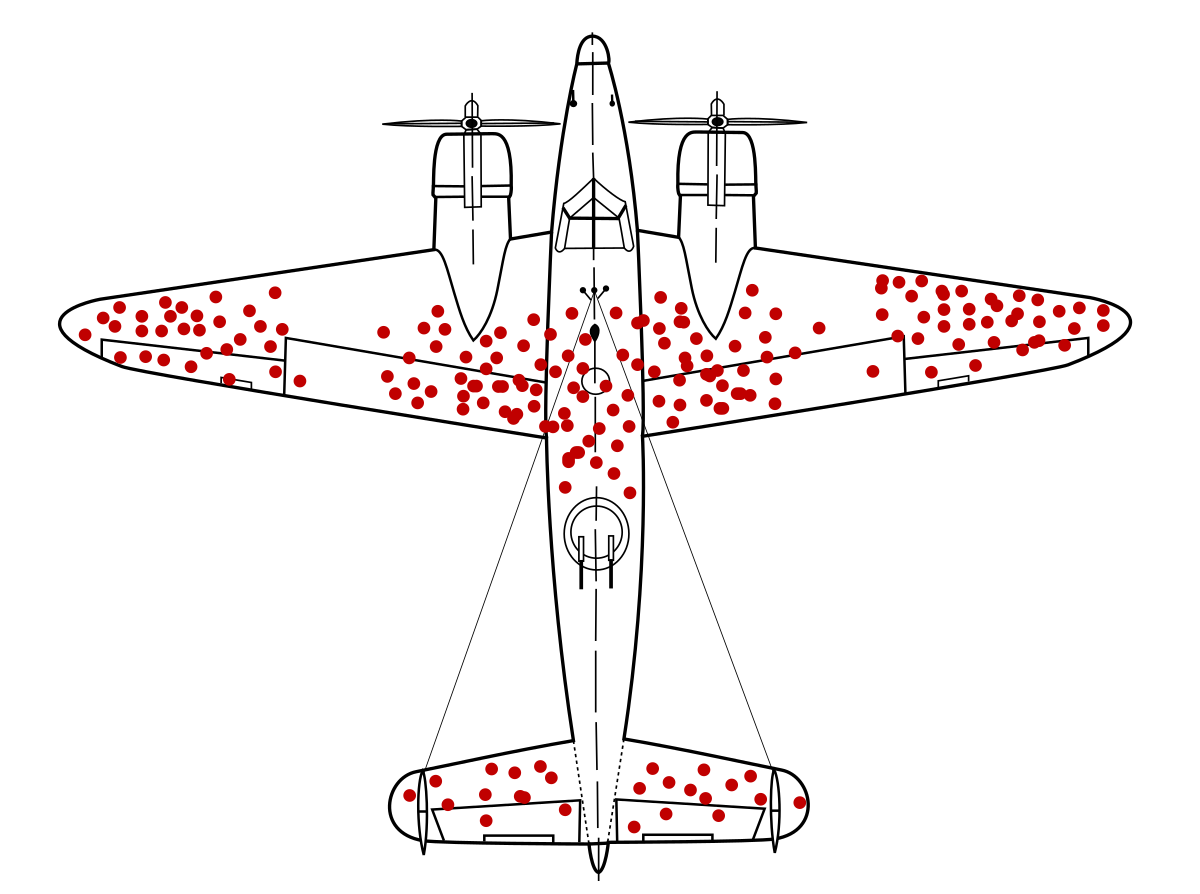
\includegraphics[width=4in,height=\textheight]{./www/bomber-holes.png}

}

\end{figure}

\end{tcolorbox}

\hypertarget{measuring-sampling-variation}{%
\section{Measuring sampling
variation}\label{measuring-sampling-variation}}

Sampling variation is a form of noise. Unlike some other forms of noise,
modeling cannot filter out sampling variation or reduce its magnitude.
Sampling variation is easiest to see by collecting multiple samples from
the same source and summarizing each one. The summaries likely will vary
from sample to sample: sampling variation.

Typically, the data frame at hand is our only sample. With no other
samples to compare it to, it may seem impossible to measure sampling
variation. In this Lesson, we will use simulations from DAGs to study
sampling variation. DAG simulations are suited to this because we can
effortlessly collect as many samples as we wish from a DAG. In
Lesson~\ref{sec-lesson-23}, we will use the knowledge gained from the
simulations to see how to measure sampling variation even when there is
only one sample.

In the spirit of starting simply, we return to \texttt{dag01}. This DAG
is \(\mathtt{x}\longrightarrow\mathtt{y}\). The causal formula setting
the value of \texttt{y} is
\texttt{y\ \textasciitilde{}\ 4\ +\ 1.5\ *\ x\ +\ exo()}.

It is crucial to remember that sampling variation is not about the
row-to-row variation in a single sample. Rather, it is about the
variation in the summary from one sample to another. So our initial
process for exploring sampling variation will be to carry out many
trials, each trial being a summary of a sample.

\hypertarget{demonstration-sampling-trials}{%
\section{Demonstration: Sampling
trials}\label{demonstration-sampling-trials}}

A single sampling trial consists of taking a random sample and computing
a sample statistic. To illustrate, here is one trial using a sample size
\(n=25\) and a simple model modification,
\texttt{y\ \textasciitilde{}\ 1}.

\begin{Shaded}
\begin{Highlighting}[]
\NormalTok{Sample }\OtherTok{\textless{}{-}} \FunctionTok{sample}\NormalTok{(dag01, }\AttributeTok{size=}\DecValTok{25}\NormalTok{) }
\NormalTok{Sample }\SpecialCharTok{\%\textgreater{}\%} 
  \FunctionTok{lm}\NormalTok{(y }\SpecialCharTok{\textasciitilde{}} \DecValTok{1}\NormalTok{, }\AttributeTok{data =}\NormalTok{ .) }\SpecialCharTok{\%\textgreater{}\%}
  \FunctionTok{coef}\NormalTok{()}
\end{Highlighting}
\end{Shaded}

\begin{verbatim}
(Intercept) 
   4.317374 
\end{verbatim}

We cannot see sampling variation directly in the above result because
there is only one trial. The sampling variation becomes evident when we
run \emph{many} trials. In each trial, a new sample (of size \(n=25\) is
taken and summarized.)

\begin{Shaded}
\begin{Highlighting}[]
\NormalTok{Trials }\OtherTok{\textless{}{-}} \FunctionTok{do}\NormalTok{(}\DecValTok{500}\NormalTok{) }\SpecialCharTok{*}\NormalTok{ \{}
\NormalTok{  Sample }\OtherTok{\textless{}{-}} \FunctionTok{sample}\NormalTok{(dag01, }\AttributeTok{size=}\DecValTok{25}\NormalTok{) }
\NormalTok{  Sample }\SpecialCharTok{\%\textgreater{}\%} 
    \FunctionTok{lm}\NormalTok{(y }\SpecialCharTok{\textasciitilde{}} \DecValTok{1}\NormalTok{, }\AttributeTok{data =}\NormalTok{ .) }\SpecialCharTok{\%\textgreater{}\%}
    \FunctionTok{coef}\NormalTok{()}
\NormalTok{\}}
\end{Highlighting}
\end{Shaded}

Graphics provide a nice way to visualize the sampling variation.
Figure~\ref{fig-sampling-distribution} shows the results from the set of
trials.

\begin{figure}

\sidecaption{\label{fig-sampling-distribution}The sampling distribution
as shown by 500 trials. Each dot is one trial where the model
specification \texttt{y\textasciitilde{}1} is fitted to a sample from
\texttt{dag01} of size \(n=25\).}

{\centering 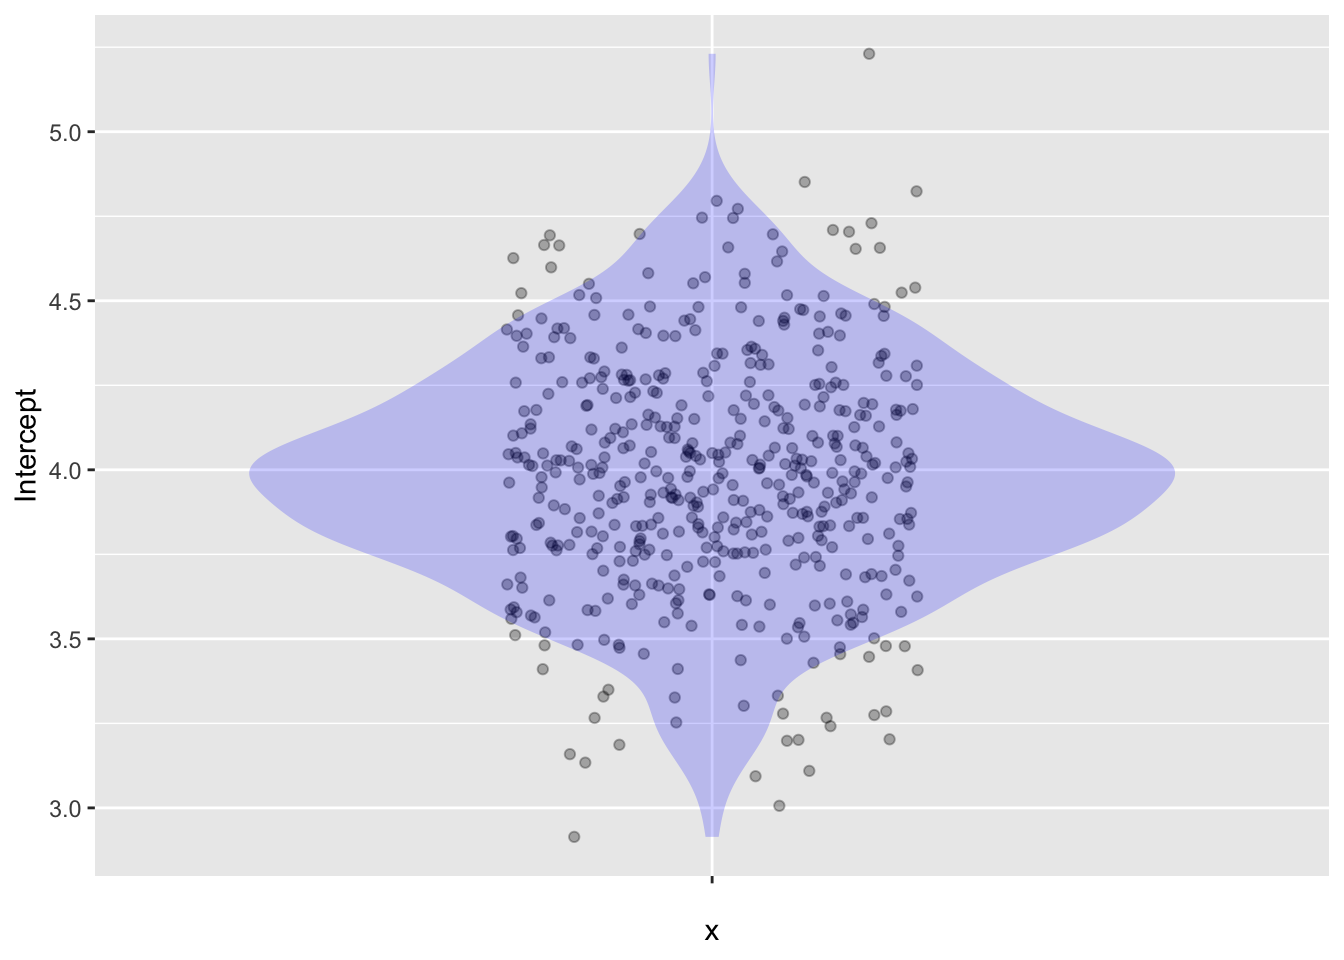
\includegraphics{./Reading-notes-lesson-22_files/figure-pdf/fig-sampling-distribution-1.pdf}

}

\end{figure}

The variance of the sampling distribution, that is, the sampling
variance, is:

\begin{Shaded}
\begin{Highlighting}[]
\NormalTok{Trials }\SpecialCharTok{\%\textgreater{}\%}
  \FunctionTok{summarize}\NormalTok{(}\AttributeTok{sampling\_variance =} \FunctionTok{var}\NormalTok{(Intercept))}
\end{Highlighting}
\end{Shaded}

\ttfamily 
\begin{tabular}{r}
\toprule
sampling\_variance\\
\midrule
0.122632\\
\bottomrule
\end{tabular} \normalfont
\bigskip

Often, statisticians prefer to use the square root of the sampling
variance, which has a technical name in statistics: the \textbf{standard
error}. The standard error is an ordinary standard deviation in a
particular context: the standard deviation of a sample of summaries. The
words \textbf{standard error} should be followed by a description of the
summary and the size of the individual samples involved. Here it would
be, ``The standard error of the Intercept coefficient from a sample of
size \(n=25\) is around 0.36.''

It is easy to confuse ``standard error'' with ``standard deviation.''
Adding to the potential confusion is another related term, the ``margin
of error.'' To avoid this confusion, we will tend to use an
\emph{interval} description of the sampling variation called the
``\textbf{confidence interval}.'' However, for the present, we will
continue with the standard error, sometimes written SE for short.

\hypertarget{se-depends-on-the-sample-size}{%
\section{SE depends on the sample
size}\label{se-depends-on-the-sample-size}}

We found an SE of 0.36 on the Intercept in a sample of size \(n=25\). We
can see how the SE depends on sample size by repeating the trials for
several different sizes, say, \(n=25\), 100, 400, 1600, 6400, 25,000,
and 100,000.

The following command estimates the SE a sample of size 400:

\begin{Shaded}
\begin{Highlighting}[]
\NormalTok{Trials }\OtherTok{\textless{}{-}} \FunctionTok{do}\NormalTok{(}\DecValTok{1000}\NormalTok{) }\SpecialCharTok{*}\NormalTok{ \{}
\NormalTok{  Sample }\OtherTok{\textless{}{-}} \FunctionTok{sample}\NormalTok{(dag01, }\AttributeTok{size=}\DecValTok{25}\NormalTok{) }
\NormalTok{  Sample }\SpecialCharTok{\%\textgreater{}\%} 
    \FunctionTok{lm}\NormalTok{(y }\SpecialCharTok{\textasciitilde{}} \DecValTok{1}\NormalTok{, }\AttributeTok{data =}\NormalTok{ .) }\SpecialCharTok{\%\textgreater{}\%}
    \FunctionTok{coef}\NormalTok{()}
\NormalTok{\}}
\NormalTok{Trials }\SpecialCharTok{\%\textgreater{}\%} \FunctionTok{summarize}\NormalTok{(}\AttributeTok{svar400 =} \FunctionTok{var}\NormalTok{(Intercept),}
                     \AttributeTok{se400 =} \FunctionTok{sd}\NormalTok{(Intercept))}
\end{Highlighting}
\end{Shaded}

\ttfamily 
\begin{tabular}{rr}
\toprule
svar400 & se400\\
\midrule
0.12766 & 0.3572954\\
\bottomrule
\end{tabular} \normalfont
\bigskip

We repeated this process for each of the other sample sizes.
Table~\ref{tbl-se-sizes} reports the results.

\hypertarget{tbl-se-sizes}{}
\ttfamily 
\begin{table}
\caption{\label{tbl-se-sizes}Results of repeating the sampling variability trials for samples of
varying sizes. }\tabularnewline

\centering
\begin{tabular}{rrr}
\toprule
n & samping\_variance & standard\_error\\
\midrule
25 & 0.1296000 & 0.3600\\
100 & 0.0361000 & 0.1900\\
400 & 0.0082810 & 0.0910\\
1600 & 0.0018490 & 0.0430\\
6400 & 0.0005290 & 0.0230\\
\addlinespace
25000 & 0.0001210 & 0.0110\\
100000 & 0.0000314 & 0.0056\\
\bottomrule
\end{tabular}
\end{table}
 \normalfont
\bigskip

There is a pattern in Table~\ref{tbl-se-sizes}. Every time we quadruple
\(n\), the sampling variance goes down by a factor of four.
Consequently, the standard error---which is just the square-root of the
sampling variance---goes down by a factor of 2, that is, \(\sqrt{4}\).
(The pattern is not exact because there is also sampling variation in
the trials, which are really just a sample of all possible trials.)

\textbf{Conclusion}: The larger the sample size, the smaller the
sampling variance. For a sample of size \(n\), the sampling variance
will be proportional to \(1/n\). Or, in terms of the standard error: For
a sample size of \(n\), the SE will be proportional to
\(1/\sqrt{\strut n}\).

\hypertarget{the-confidence-interval}{%
\section{The confidence interval}\label{the-confidence-interval}}

The ``confidence interval'' is a more user-friendly format than SE for
describing the amount of sampling variation. Being an interval, write it
either as {[}lower, upper{]} or center\(\pm\)half-width. These styles
are equivalent; both styles are correct. (The preferred style can depend
on the field or the journal publishing the report.)

In practice, confidence intervals are calculated using special-purpose
software such as the \texttt{conf\_interval()} function, for instance:

\begin{Shaded}
\begin{Highlighting}[]
\NormalTok{Hill\_racing }\SpecialCharTok{\%\textgreater{}\%} 
  \FunctionTok{lm}\NormalTok{(time }\SpecialCharTok{\textasciitilde{}}\NormalTok{ distance }\SpecialCharTok{+}\NormalTok{ climb, }\AttributeTok{data=}\NormalTok{.) }\SpecialCharTok{\%\textgreater{}\%} 
  \FunctionTok{conf\_interval}\NormalTok{()}
\end{Highlighting}
\end{Shaded}

\ttfamily 
\begin{tabular}{lrr}
\toprule
term & .lwr & .upr\\
\midrule
(Intercept) & -533.432471 & -406.521402\\
distance & 246.387096 & 261.229494\\
climb & 2.493307 & 2.726209\\
\bottomrule
\end{tabular} \normalfont
\bigskip

Notice that there is a separate confidence interval for each model
coefficient. The sampling variation is essentially the same, but that
variation appears different when translated to the various coefficients'
units.

\begin{tcolorbox}[enhanced jigsaw, colbacktitle=quarto-callout-warning-color!10!white, breakable, opacitybacktitle=0.6, colback=white, left=2mm, arc=.35mm, colframe=quarto-callout-warning-color-frame, coltitle=black, toprule=.15mm, opacityback=0, leftrule=.75mm, bottomtitle=1mm, toptitle=1mm, titlerule=0mm, title=\textcolor{quarto-callout-warning-color}{\faExclamationTriangle}\hspace{0.5em}{Demonstration: How many digits?}, rightrule=.15mm, bottomrule=.15mm]

The confidence intervals on the model
\texttt{time\ \textasciitilde{}\ distance\ +\ climb}, report the results
to many digits. Such a report is appropriate for further calculations
that might need doing, but it is usually not appropriate for a human
reader.

To know how many digits are worth reporting to humans, look toward the
standard error. The standard error is a part of a different kind of
summary of a model: the ``regression report.'' We will only need to look
at regression reports in the last few Lessons of the course. Here we
want to point out how many digits are worth reporting to humans. That
requires looking at the standard error itself.

Previously, we looked at the confidence intervals on coefficients from
the \texttt{Hill\_racing} model. Now we look at the regression summary,
which contains the information on sampling variation in a different
format.

\begin{Shaded}
\begin{Highlighting}[]
\NormalTok{Hill\_racing }\SpecialCharTok{\%\textgreater{}\%} 
  \FunctionTok{lm}\NormalTok{(time }\SpecialCharTok{\textasciitilde{}}\NormalTok{ distance }\SpecialCharTok{+}\NormalTok{ climb, }\AttributeTok{data=}\NormalTok{.) }\SpecialCharTok{\%\textgreater{}\%} 
  \FunctionTok{regression\_summary}\NormalTok{()}
\end{Highlighting}
\end{Shaded}

\ttfamily 
\begin{tabular}{lrrrr}
\toprule
term & estimate & std.error & statistic & p.value\\
\midrule
(Intercept) & -469.976937 & 32.3582241 & -14.52419 & 0\\
distance & 253.808295 & 3.7843322 & 67.06819 & 0\\
climb & 2.609758 & 0.0593826 & 43.94821 & 0\\
\bottomrule
\end{tabular} \normalfont
\bigskip

Each coefficient's standard error appears in the \texttt{std.error}
column of the regression summary.

For the human reader, only the first two significant digits of the
standard error are worth reporting. (This is true regardless of the data
and model design.) Here, the SE is 32 for the Intercept, 3.8 for the
distance coefficient, and 0.059 for the climb coefficient. The
confidence interval will be the coefficient (column labeled
\texttt{estimate}) plus or minus ``twice'' the \texttt{std.error}. It is
appropriate to round the confidence interval (for a human reader) to the
first two significant digits of the standard error.

For example, the confidence interval on the distance coefficient will be
\(253.808295 \pm 2 \times 3.78433220\). Keep only the digits before the
first two significant digits of the SE, so the reported interval can be
\(253.8 \pm 3.8\).

\end{tcolorbox}

\hypertarget{sec-lesson-23}{%
\chapter{Confidence intervals from a single
sample}\label{sec-lesson-23}}

Lesson~\ref{sec-lesson-21} introduced separating data into components:
signal and noise. The \emph{signal} is a summary of the data that tells
us something we want to know. Often, the signal will be one or more
coefficients from a regression report, but it might be something as
simple as the mean, median, or standard deviation of a variable in a
data frame.

The \emph{noise} comes into the data from various sources: e.g., error
in measurement or a data-entry blunder. Another source of noise is
omnipresent (except in a perfect census): sampling variation as
discussed in Lesson~\ref{sec-lesson-22}. Sampling variation arises
because the particular sample we happen to be working with reflects, to
some extent, the play of luck. If we had happened to select another
sample, the results would be different.

In general, whenever we measure something, say the altitude of a plane
or the fuel economy of a car, it is helpful to know the
``\textbf{precision}'' of that estimate. It would be disastrous if the
measured difference in altitude of two planes flying toward a common
point were imprecise to the extent that the difference might actually be
zero! Knowing the precision of the altitude measurement enables us to
space the place in a safe way.

One way to think about precision is in terms of repeatability. If we
make multiple measurements of the same object in the same manner, the
precision is the degree to which those measurements vary from one
another. With the instrumentation used for physical measurements, the
precision of individual measurements is estimated by repeated measuring
the same thing. Likewise, in statistical summaries, the precision is
related to sampling variation.

In Lesson~\ref{sec-lesson-22}, we repeated trials over and over again to
gain some feeling for sampling variation. We quantified the
repeatability in any of several closely related ways: the sampling
variance or its square root (the ``standard error'') or a ``margin of
error'' or a ``confidence interval.'' Our experiments with simulations
demonstrated an important property of sampling variation: the amount of
sampling variation depends on the sample size \(n\). In particular, the
sampling variance gets smaller as \(n\) increases in proportion to
\(1/n\). (Consequently, the standard error gets smaller in proportion to
\(1/\sqrt{n}\).)

It is time to take off the DAG simulation training wheels and measure
sampling variation from a \emph{single} data frame. Our first approach
will be to turn the single sample into several smaller samples:
subsampling. Later, we will turn to another technique, resampling, which
draws a sample of full size from the data frame. Sometimes, in
particular with regression models, it is possible to calculate the
sampling variation from a formula, allowing software to carry out and
report the calculations automatically.

\hypertarget{sec-subsampling}{%
\section{Subsampling}\label{sec-subsampling}}

To ``subsample'' means to draw a smaller sample from a large one.
``Small'' and ``large'' are relative. For our example, we turn to the
\texttt{TenMileRace} data frame containing the record of thousands of
runners' times in a race, along with basic information about each
runner. There are many ways we could summarize \texttt{TenMileRace.} Any
summary would do for the example. We will summarize the relationship
between the runners' ages and their start-to-finish times (variable
\texttt{net}), that is, \texttt{net\ \textasciitilde{}\ age}. To avoid
the complexity of a runner's improvement with age followed by a decline,
we will limit the study to people over 40.

\begin{Shaded}
\begin{Highlighting}[]
\NormalTok{TenMileRace }\SpecialCharTok{\%\textgreater{}\%} \FunctionTok{filter}\NormalTok{(age }\SpecialCharTok{\textgreater{}} \DecValTok{40}\NormalTok{) }\SpecialCharTok{\%\textgreater{}\%}
  \FunctionTok{lm}\NormalTok{(net }\SpecialCharTok{\textasciitilde{}}\NormalTok{ age, }\AttributeTok{data =}\NormalTok{ .) }\SpecialCharTok{\%\textgreater{}\%} \FunctionTok{coef}\NormalTok{()}
\end{Highlighting}
\end{Shaded}

\begin{verbatim}
(Intercept)         age 
 4278.21279    28.13517 
\end{verbatim}

The units of \texttt{net} are seconds, and the units of \texttt{age} are
years. The model coefficient on \texttt{age} tells us how the
\texttt{net} time changes for each additional year of \texttt{age}:
seconds per year. Using the entire data frame, we see that the time to
run the race gets longer by about 28 seconds per year. So a 45-year-old
runner who completed this year's 10-mile race in 3900 seconds (about 9.2
mph, a pretty good pace!) might expect that, in ten years, when she is
55 years old, her time will be longer by 280 seconds.

It would be asinine to report the ten-year change as 281.3517 seconds.
The runner's time ten years from now will be influenced by the weather,
crowding, the course conditions, whether she finds a good pace runner,
the training regime, improvements in shoe technology, injuries, and
illnesses, among other factors. There is little or nothing we can say
from the \texttt{TenMileRace} data about such factors.

There's also sampling variation. There are 2898 people older than 40 in
the \texttt{TenMileRace} data frame. The way the data was collected
(radio-frequency interrogation of a dongle on the runner's shoe)
suggests that the data is a census of finishers. However, it is also
fair to treat it as a sample of the kind of people who run such races.
People might have been interested in running but had a schedule
conflict, lived too far away, or missed their train to the start line in
the city.

We see sampling variation by comparing multiple samples. To create those
multiple samples from \texttt{TenMileRace}, we will draw, at random,
subsamples of, say, one-tenth the size of the whole, that is, \(n=290\)

\begin{Shaded}
\begin{Highlighting}[]
\NormalTok{Over40 }\OtherTok{\textless{}{-}}\NormalTok{ TenMileRace }\SpecialCharTok{\%\textgreater{}\%} \FunctionTok{filter}\NormalTok{(age }\SpecialCharTok{\textgreater{}} \DecValTok{40}\NormalTok{)}
\FunctionTok{lm}\NormalTok{(time }\SpecialCharTok{\textasciitilde{}}\NormalTok{ age, }\AttributeTok{data =}\NormalTok{ Over40 }\SpecialCharTok{\%\textgreater{}\%} \FunctionTok{sample}\NormalTok{(}\AttributeTok{size=}\DecValTok{290}\NormalTok{)) }\SpecialCharTok{\%\textgreater{}\%} \FunctionTok{coef}\NormalTok{()}
\end{Highlighting}
\end{Shaded}

\begin{verbatim}
(Intercept)         age 
 4366.31506    31.19676 
\end{verbatim}

\begin{Shaded}
\begin{Highlighting}[]
\FunctionTok{lm}\NormalTok{(time }\SpecialCharTok{\textasciitilde{}}\NormalTok{ age, }\AttributeTok{data =}\NormalTok{ Over40 }\SpecialCharTok{\%\textgreater{}\%} \FunctionTok{sample}\NormalTok{(}\AttributeTok{size=}\DecValTok{290}\NormalTok{)) }\SpecialCharTok{\%\textgreater{}\%} \FunctionTok{coef}\NormalTok{()}
\end{Highlighting}
\end{Shaded}

\begin{verbatim}
(Intercept)         age 
 4138.10256    35.16787 
\end{verbatim}

The age coefficients from these two subsampling trials differ one from
the other by about 0.5 seconds. To get a more systematic view, run more
trials:

\begin{Shaded}
\begin{Highlighting}[]
\CommentTok{\# a sample of summaries}
\NormalTok{Trials }\OtherTok{\textless{}{-}} \FunctionTok{do}\NormalTok{(}\DecValTok{1000}\NormalTok{) }\SpecialCharTok{*}\NormalTok{ \{}
  \FunctionTok{lm}\NormalTok{(time }\SpecialCharTok{\textasciitilde{}}\NormalTok{ age, }\AttributeTok{data =} \FunctionTok{sample}\NormalTok{(Over40, }\AttributeTok{size=}\DecValTok{290}\NormalTok{)) }\SpecialCharTok{\%\textgreater{}\%} \FunctionTok{coef}\NormalTok{()}
\NormalTok{\}}
\CommentTok{\# a summary of the sample of summaries}
\NormalTok{Trials }\SpecialCharTok{\%\textgreater{}\%}
\NormalTok{  dplyr}\SpecialCharTok{::}\FunctionTok{summarize}\NormalTok{(}\AttributeTok{se =} \FunctionTok{sd}\NormalTok{(age))}
\end{Highlighting}
\end{Shaded}

\ttfamily 
\begin{tabular}{r}
\toprule
se\\
\midrule
8.986386\\
\bottomrule
\end{tabular} \normalfont
\bigskip

We used the name \texttt{se} for the summary of samples of summaries
because what we have calculated is the standard error of the age
coefficient from samples of size \(n=290\).

In Lesson~\ref{sec-lesson-22} we saw that the standard error is
proportional to \(1/\sqrt{\strut n}\), where \(n\) is the sample size.
From the subsamples, know that the SE for \(n=290\) is about 9.0
seconds. This tells us that the SE for the full \(n=2898\) samples would
be about \(9.0 \frac{\sqrt{290}}{\sqrt{2898}} = 2.85\).

So the interval summary of the \texttt{age} coefficient---the
\emph{confidence interval}--- is
\[\underbrace{28.1}_\text{age coef.} \pm 2\times\!\!\!\!\!\!\! \underbrace{2.85}_\text{standard error} =\ \ \ \  28.1 \pm\!\!\!\!\!\!\!\! \underbrace{5.6}_\text{margin of error}\ \  \text{or, equivalently, 22.6 to 33.6}\]

\hypertarget{bootstrapping}{%
\section{Bootstrapping}\label{bootstrapping}}

There is a trick, called ``\textbf{resampling},'' to generate a random
subsample of a data frame with the same \(n\) as the data frame: draw
the new sample randomly from the original sample \textbf{with
replacement}. An example will suffice to show what the ``with
replacement'' does:

\begin{Shaded}
\begin{Highlighting}[]
\NormalTok{example }\OtherTok{\textless{}{-}} \FunctionTok{c}\NormalTok{(}\DecValTok{1}\NormalTok{,}\DecValTok{2}\NormalTok{,}\DecValTok{3}\NormalTok{,}\DecValTok{4}\NormalTok{,}\DecValTok{5}\NormalTok{)}
\CommentTok{\# without replacement}
\FunctionTok{sample}\NormalTok{(example)}
\end{Highlighting}
\end{Shaded}

\begin{verbatim}
[1] 1 4 3 5 2
\end{verbatim}

\begin{Shaded}
\begin{Highlighting}[]
\CommentTok{\# now, with replacement}
\FunctionTok{sample}\NormalTok{(example, }\AttributeTok{replace=}\ConstantTok{TRUE}\NormalTok{)}
\end{Highlighting}
\end{Shaded}

\begin{verbatim}
[1] 2 4 3 3 5
\end{verbatim}

\begin{Shaded}
\begin{Highlighting}[]
\FunctionTok{sample}\NormalTok{(example, }\AttributeTok{replace=}\ConstantTok{TRUE}\NormalTok{)}
\end{Highlighting}
\end{Shaded}

\begin{verbatim}
[1] 3 5 4 4 4
\end{verbatim}

\begin{Shaded}
\begin{Highlighting}[]
\FunctionTok{sample}\NormalTok{(example, }\AttributeTok{replace=}\ConstantTok{TRUE}\NormalTok{)}
\end{Highlighting}
\end{Shaded}

\begin{verbatim}
[1] 1 1 2 2 3
\end{verbatim}

\begin{Shaded}
\begin{Highlighting}[]
\FunctionTok{sample}\NormalTok{(example, }\AttributeTok{replace=}\ConstantTok{TRUE}\NormalTok{)}
\end{Highlighting}
\end{Shaded}

\begin{verbatim}
[1] 4 3 1 4 5
\end{verbatim}

The ``with replacement'' leads to the possibility that some values will
be repeated two or more times and other values will be left out
entirely.

The calculation of the SE using resampling is called
``\textbf{bootstrapping}.''

\begin{tcolorbox}[enhanced jigsaw, colbacktitle=quarto-callout-warning-color!10!white, breakable, opacitybacktitle=0.6, colback=white, left=2mm, arc=.35mm, colframe=quarto-callout-warning-color-frame, coltitle=black, toprule=.15mm, opacityback=0, leftrule=.75mm, bottomtitle=1mm, toptitle=1mm, titlerule=0mm, title=\textcolor{quarto-callout-warning-color}{\faExclamationTriangle}\hspace{0.5em}{Demonstration: Bootstrapping the standard error}, rightrule=.15mm, bottomrule=.15mm]

We will apply bootstrapping to find the standard error of the
\texttt{age} coefficient from the model
\texttt{time\ \textasciitilde{}\ age} fit to the \texttt{Over40} data
frame.

There are two steps:

\begin{enumerate}
\def\labelenumi{\arabic{enumi}.}
\item
  Run many trials, each of which fits the model
  \texttt{time\ \textasciitilde{}\ age} using \texttt{lm()}. From trial
  to trial, the data used for fitting is a resampling of the
  \texttt{Over40} data frame. The result of each trial is the
  coefficients from the model.
\item
  Summarize the trials with the standard deviation of the \texttt{age}
  coefficients.
\end{enumerate}

\begin{Shaded}
\begin{Highlighting}[]
\CommentTok{\# run many trials}
\NormalTok{Trials }\OtherTok{\textless{}{-}} \FunctionTok{do}\NormalTok{(}\DecValTok{1000}\NormalTok{) }\SpecialCharTok{*}\NormalTok{ \{}
  \FunctionTok{lm}\NormalTok{(time }\SpecialCharTok{\textasciitilde{}}\NormalTok{ age, }\AttributeTok{data =} \FunctionTok{sample}\NormalTok{(Over40, }\AttributeTok{replace=}\ConstantTok{TRUE}\NormalTok{)) }\SpecialCharTok{\%\textgreater{}\%} 
       \FunctionTok{coef}\NormalTok{()}
\NormalTok{\}}
\CommentTok{\# summarize the trials to find the SE}
\NormalTok{Trials }\SpecialCharTok{\%\textgreater{}\%} \FunctionTok{summarize}\NormalTok{(}\AttributeTok{se =} \FunctionTok{sd}\NormalTok{(age))}
\end{Highlighting}
\end{Shaded}

\ttfamily 
\begin{tabular}{r}
\toprule
se\\
\midrule
2.859483\\
\bottomrule
\end{tabular} \normalfont
\bigskip

\end{tcolorbox}

\hypertarget{confidence-intervals-from-software}{%
\section{Confidence intervals from
software}\label{confidence-intervals-from-software}}

The same mathematical process that powers regression modeling software
such as \texttt{lm()} can be used to compute standard errors for model
coefficients as part of the fitting process. So, for regression models,
finding a confidence interval is just a matter of asking for it.

{[}Note: Experienced R users will know that the ``standard'' function
for calculating confidence intervals is \texttt{confint()}, which is
used in exactly the same manner as \texttt{conf\_interval()}.
Regrettably, \texttt{confint()} does not create a data frame. In keeping
with these Lessons use of data wrangling, the \texttt{conf\_interval()}
from the \texttt{\{math300\}} package reformats the output of
\texttt{confint()} into a data frame.{]}

There are several ways to do the asking. In R, the
\texttt{conf\_interval()} function makes it easy to extract the
confidence intervals on each coefficient from a model. For example:

\begin{Shaded}
\begin{Highlighting}[]
\FunctionTok{lm}\NormalTok{(net }\SpecialCharTok{\textasciitilde{}}\NormalTok{ age }\SpecialCharTok{+}\NormalTok{ sex, }\AttributeTok{data =}\NormalTok{ TenMileRace) }\SpecialCharTok{|\textgreater{}} \FunctionTok{conf\_interval}\NormalTok{() }
\end{Highlighting}
\end{Shaded}

\ttfamily 
\begin{tabular}{lrr}
\toprule
term & .lwr & .upr\\
\midrule
(Intercept) & 5270.45170 & 5407.85920\\
age & 15.04242 & 18.74483\\
sexM & -765.85978 & -687.37917\\
\bottomrule
\end{tabular} \normalfont
\bigskip

Each row of the result reports the confidence interval for one
coefficient from the model.

\hypertarget{sec-lesson-24}{%
\chapter{Effect size}\label{sec-lesson-24}}

Regression modeling and confidence intervals provide a substantial
toolbox to support statistical thinking. This Lesson starts to develop
methods using modeling to inform decision-making. Decision-making takes
many guises: whether to administer medicine, change a budget, raise or
lower a price, respond to an evolving situation, and so on.

A useful simplification splits support for decision-making into two
broad categories.

\begin{enumerate}
\def\labelenumi{\arabic{enumi}.}
\item
  \textbf{Making a prediction} for an individual choice. The need for
  predictions arises in both mundane and critical settings. For
  instance, an airline needs to set prices. They want to maximize
  revenue. Higher prices will bring in more money per seat but may
  reduce the number of people flying. To make the pricing decision, the
  airline needs a prediction about what the demand will be for those
  seats, which may vary based on price, day of the week, time of day,
  time of year, origin and destination of the flight, and so on. Another
  example: Merchants and social media sites must choose what products or
  posts to display to a viewer. Merchants have many products, and social
  media has many news feeds, tweets, and competing blog entries. The
  people who manage these websites want to promote the products or
  postings most likely to cause a viewer to respond. To identify viable
  products or postings, the site managers construct predictive models
  based on earlier viewers' choices. We will study prediction models in
  Lessons 25 and 26,
\item
  \textbf{Intervening} in a system. Such interventions occur on both
  grand scales and small: changes in government policies such as funding
  for preschool education or subsidies for renewable energy, closing a
  road to redirect traffic or opening a new highway or bus line,
  changing the minimum wage, etc. Before making such interventions, it
  is wise to know what the consequences are likely to be. Figuring this
  out is often a matter of understanding how the system works: what
  causes what. As interventions often affect multiple individuals,
  influencing the overall trend of the effect across individuals might
  be the goal instead of predicting how each individual will be
  affected.
\end{enumerate}

This Lesson focuses on ``\textbf{effect size},'' a measure of how
changing an explanatory variable will play out in the response variable.
Built into the previous sentence is an assumption that the explanatory
variable \emph{causes} the response variable. In Lessons 28 through 31,
we will look into ways to make responsible claims about whether a
connection between variables is causal. Here, we will focus on the
calculation and interpretation of effect size.

\hypertarget{effect-size-input-to-output}{%
\section{Effect size: Input to
output}\label{effect-size-input-to-output}}

An intervention changes something in the world. Some examples are the
budget for a program, the dose of a medicine, or the fuel flow into an
engine. The thing being changed is the \emph{input}. In response,
something else in the world changes, for instance, the reading ability
of students, the patient's serotonin levels (a neurotransmitter), or the
power output from the engine. The thing that changes in response to the
change in input is called the ``output.''

``\textbf{Effect size}'' describes the change in the output with respect
to the change in the input. The simplest case is when the output is a
quantitative variable. In this case, the change in the output is a
difference between two numbers. The form of the effect size depends on
the input type. For example, for a quantitative input, the effect size
will be a \emph{ratio}, that is, a rate. (For calculus students: the
effect size is a derivative of the output with respect to the input.)

To measure an effect size from data, construct a model with the output
as the response variable and the input as an explanatory variable.

\begin{tcolorbox}[enhanced jigsaw, colbacktitle=quarto-callout-note-color!10!white, breakable, opacitybacktitle=0.6, colback=white, left=2mm, arc=.35mm, colframe=quarto-callout-note-color-frame, coltitle=black, toprule=.15mm, opacityback=0, leftrule=.75mm, bottomtitle=1mm, toptitle=1mm, titlerule=0mm, title=\textcolor{quarto-callout-note-color}{\faInfo}\hspace{0.5em}{Example: Fuel economy}, rightrule=.15mm, bottomrule=.15mm]

A person buying a car typically has multiple objectives in mind. Perhaps
the buyer is deciding whether to order a more powerful engine. This
decision has consequences, including a reduction in fuel economy. The
decision variable---the engine size---is the input; the fuel economy is
the output.

Since both input and output are quantitative, the effect size will be a
rate: change in fuel economy per change in engine size. To inform a
decision, use data such as the \texttt{math300::MPG} data frame, which
compares various car models. \texttt{MPG} records the engine size in
terms of \texttt{displacement}, in liters. Fuel economy is listed in
miles per gallon, differently for city versus highway driving.

The buyer is debating between a 2-liter and a 3-liter engine. Most
driving will be in the city. To calculate the effect size, first build a
model with the output (\texttt{mpg\_city}) as the response variable and
the input (\texttt{displacement}) as an explanatory variable.

\begin{Shaded}
\begin{Highlighting}[]
\NormalTok{Mod }\OtherTok{\textless{}{-}} \FunctionTok{lm}\NormalTok{(mpg\_city }\SpecialCharTok{\textasciitilde{}}\NormalTok{ displacement, }\AttributeTok{data=}\NormalTok{MPG)}
\end{Highlighting}
\end{Shaded}

Second, evaluate that model for the range of inputs under consideration.

\begin{Shaded}
\begin{Highlighting}[]
\FunctionTok{model\_eval}\NormalTok{(Mod, }\AttributeTok{displacement=}\FunctionTok{c}\NormalTok{(}\DecValTok{2}\NormalTok{, }\DecValTok{3}\NormalTok{))}
\end{Highlighting}
\end{Shaded}

\ttfamily 
\begin{tabular}{rrrr}
\toprule
displacement & .output & .lwr & .upr\\
\midrule
2 & 24.01437 & 15.91915 & 32.10959\\
3 & 20.86976 & 12.77698 & 28.96254\\
\bottomrule
\end{tabular} \normalfont
\bigskip

The change in the input from 3 liters displacement to 2 liters leads to
a change in fuel economy of \(24.0 - 20.9 = -3.1\) miles per gallon. The
change in displacement is \(3 - 2 = 1\) liters. The effect size is the
ratio between the output change and the input change. Here, that is -3.1
miles per gallon per liter.

The decision-maker may be more concerned about the cost of driving than
with the miles per gallon. Then the appropriate response variable might
be \texttt{EPA\_fuel\_cost,} denominated in dollars per year.

\begin{Shaded}
\begin{Highlighting}[]
\NormalTok{Mod2 }\OtherTok{\textless{}{-}} \FunctionTok{lm}\NormalTok{(EPA\_fuel\_cost }\SpecialCharTok{\textasciitilde{}}\NormalTok{ displacement, }\AttributeTok{data=}\NormalTok{MPG)}
\FunctionTok{model\_eval}\NormalTok{(Mod2, }\AttributeTok{displacement=}\FunctionTok{c}\NormalTok{(}\DecValTok{2}\NormalTok{, }\DecValTok{3}\NormalTok{))}
\end{Highlighting}
\end{Shaded}

\ttfamily 
\begin{tabular}{rrrr}
\toprule
displacement & .output & .lwr & .upr\\
\midrule
2 & 1585.887 & 1000.649 & 2171.125\\
3 & 1882.534 & 1297.473 & 2467.596\\
\bottomrule
\end{tabular} \normalfont
\bigskip

The change in output is about \$300 per year. However, the change in
input is still 1 liter. The effect size is, therefore, \$300 per year
per liter.

\end{tcolorbox}

Some decision variables are categorical. For instance, the buyer might
like the idea of an engine that automatically turns off when the car is
stopped at a light or in traffic. The \texttt{start\_stop} variable,
which has categorical levels ``Yes'' and ``No,'' records whether the car
has this feature. Effect size estimation is slightly different when the
input is categorical rather than quantitative. Still, build a model and
compare the change in output to the change in input:

\begin{Shaded}
\begin{Highlighting}[]
\NormalTok{Mod3 }\OtherTok{\textless{}{-}} \FunctionTok{lm}\NormalTok{(EPA\_fuel\_cost }\SpecialCharTok{\textasciitilde{}}\NormalTok{ start\_stop, }\AttributeTok{data=}\NormalTok{MPG)}
\FunctionTok{model\_eval}\NormalTok{(Mod3, }\AttributeTok{start\_stop=}\FunctionTok{c}\NormalTok{(}\StringTok{"No"}\NormalTok{, }\StringTok{"Yes"}\NormalTok{))}
\end{Highlighting}
\end{Shaded}

\ttfamily 
\begin{tabular}{lrrr}
\toprule
start\_stop & .output & .lwr & .upr\\
\midrule
No & 1872.193 & 916.0164 & 2828.369\\
Yes & 1945.194 & 989.0637 & 2901.324\\
\bottomrule
\end{tabular} \normalfont
\bigskip

In this case, the change in output is \$73 per year; the change in input
is ``Yes'' - ``No.'' But, of course, it is meaningless to subtract one
categorical level from another. Consequently, the effect size of
\texttt{start\_stop} on fuel cost cannot be quantified as a ratio. So,
instead, the effect size is simply the difference in the output: a \$73
per year increase with the Start/Stop feature.

The statistical thinker knows to pay attention to whether a calculated
result makes sense. It seems unlikely that the Start/Stop feature causes
more fuel to be consumed. Was there an error? Perhaps we did the
subtraction backward? Check the report from \texttt{model\_eval()} to
make sure.

Here, the problem is not arithmetic. However, there is another
possibility. It might be that manufacturers include the Start/Stop
feature with big cars but not little ones. Then, even if Start/Stop
might save gas when everything else is held constant, because the big
cars use more fuel than little cars, it only \emph{appears} that
Start/Stop hurts fuel economy. This theory is, at this point,
speculation: a hypothesis. Such a mixture of effects---big versus small
car mixed with availability of Start/Stop---is called
``\textbf{confounding}.'' In Lessons 28 through 30, we discuss
identifying and dealing with possible confounding.

\begin{tcolorbox}[enhanced jigsaw, colbacktitle=quarto-callout-warning-color!10!white, breakable, opacitybacktitle=0.6, colback=white, left=2mm, arc=.35mm, colframe=quarto-callout-warning-color-frame, coltitle=black, toprule=.15mm, opacityback=0, leftrule=.75mm, bottomtitle=1mm, toptitle=1mm, titlerule=0mm, title=\textcolor{quarto-callout-warning-color}{\faExclamationTriangle}\hspace{0.5em}{Confounding?}, rightrule=.15mm, bottomrule=.15mm]

The surprising positive effect size of the Start/Stop feature caused a
double take and led us to think of ways to make sense of the result.
Right now, we simply have a hypothesis that Start/Stop is associated
with bigger cars. (We will check that out in a little bit.)

The effect size of annual fuel cost with respect to engine displacement,
\$300 per year per liter, did not surprise us. Perhaps it should have.
After all, larger vehicles tend to have larger engines. This
relationship might lead to confounding between vehicle size and engine
displacement. We think we are looking at engine displacement, but
instead, the effect might be due to vehicle size. Again, just a
hypothesis at this point. The statistical thinker knows to consider
possible confounding from the start.

\end{tcolorbox}

\hypertarget{categorical-outputs}{%
\section{Categorical outputs}\label{categorical-outputs}}

Sometimes the relevant effect size involves a categorical output
variable. A case in point is the possible confounding of the Start/Stop
feature with vehicle size. To investigate this, we should build a model
with Start/Stop as the output and vehicle size as the input.

In this case, the issue of whether vehicle size causes Start/Stop is not
essential. We are not concerned with the decisions made by automobile
designers so much as with the possible confounding.

When the output variable is categorical, it is not reasonable to
calculate the change in output as the difference in categories. As
before, ``Yes'' - ``No'' is not a number. Still, there is a meaningful
and helpful way to quantify a change in a categorical output.

The essential insight is quantifying the change in output in terms of
probabilities. For instance, a small effect size would reflect a slight
chance of the output changing from one level to another.

The appropriate model type for a categorical output is to transform the
output to a zero-one variable, as introduced in
Lesson~\ref{sec-lesson-19}. We will present this in a demonstration here
and return to the topic more fully in Lesson 34.

\begin{tcolorbox}[enhanced jigsaw, colbacktitle=quarto-callout-warning-color!10!white, breakable, opacitybacktitle=0.6, colback=white, left=2mm, arc=.35mm, colframe=quarto-callout-warning-color-frame, coltitle=black, toprule=.15mm, opacityback=0, leftrule=.75mm, bottomtitle=1mm, toptitle=1mm, titlerule=0mm, title=\textcolor{quarto-callout-warning-color}{\faExclamationTriangle}\hspace{0.5em}{Demonstration: Start/Stop and vehicle size}, rightrule=.15mm, bottomrule=.15mm]

As described earlier, we are interested in the possibility that
Start/Stop is available mainly on large, higher-fuel-consumption cars.
If so, that would explain why the effect size we calculated of fuel cost
with respect to Start/Stop was positive.

The model we build will have a zero-one encoding of Start/Stop as the
response and the vehicle's fuel cost as the explanatory variable.

\begin{Shaded}
\begin{Highlighting}[]
\NormalTok{MPG }\OtherTok{\textless{}{-}}\NormalTok{ MPG }\SpecialCharTok{\%\textgreater{}\%} 
    \FunctionTok{mutate}\NormalTok{(}\AttributeTok{has\_start\_stop =} \FunctionTok{zero\_one}\NormalTok{(start\_stop, }\AttributeTok{one=}\StringTok{"Yes"}\NormalTok{))}
\NormalTok{Mod4 }\OtherTok{\textless{}{-}} \FunctionTok{lm}\NormalTok{(has\_start\_stop }\SpecialCharTok{\textasciitilde{}}\NormalTok{ EPA\_fuel\_cost, }\AttributeTok{data =}\NormalTok{ MPG)}
\FunctionTok{model\_eval}\NormalTok{(Mod4, }\AttributeTok{EPA\_fuel\_cost=}\FunctionTok{c}\NormalTok{(}\DecValTok{1600}\NormalTok{, }\DecValTok{2000}\NormalTok{))}
\end{Highlighting}
\end{Shaded}

\ttfamily 
\begin{tabular}{rrrr}
\toprule
EPA\_fuel\_cost & .output & .lwr & .upr\\
\midrule
1600 & 0.4901341 & -0.4891981 & 1.469466\\
2000 & 0.5207835 & -0.4583924 & 1.499959\\
\bottomrule
\end{tabular} \normalfont
\bigskip

The \texttt{.output} here is interpreted as a \emph{probability} of
\texttt{start\_stop} having the value ``Yes.'' (That is because we set
\texttt{one="Yes"} in the \texttt{zero\_one()} conversion.) The
\texttt{model\_eval()} report indicates \$400 per year increase in fuel
cost is associated with a three percentage point increase in the
probability of a vehicle having a Start/Stop feature. That is a small
effect, so we see little support for our hypothesis that Start/Stop
tends to be installed on larger, more fuel-efficient vehicles.

\end{tcolorbox}

\hypertarget{multiple-explanatory-variables}{%
\section{Multiple explanatory
variables}\label{multiple-explanatory-variables}}

When a model has more than one explanatory variable, each has a
different effect size.

As an example, consider the price of books. We have some data that might
be informative, \texttt{moderndive::amazon\_books}. What is the effect
size of page count on price. The appropriate model here is
\texttt{list\_price\ \textasciitilde{}\ num\_pages}. The effect size is
easy to compute:

\begin{Shaded}
\begin{Highlighting}[]
\NormalTok{Mod1 }\OtherTok{\textless{}{-}} \FunctionTok{lm}\NormalTok{(list\_price }\SpecialCharTok{\textasciitilde{}}\NormalTok{ num\_pages, }\AttributeTok{data =}\NormalTok{ moderndive}\SpecialCharTok{::}\NormalTok{amazon\_books)}
\FunctionTok{model\_eval}\NormalTok{(Mod1, }\AttributeTok{num\_pages =} \FunctionTok{c}\NormalTok{(}\DecValTok{200}\NormalTok{, }\DecValTok{400}\NormalTok{))}
\end{Highlighting}
\end{Shaded}

\ttfamily 
\begin{tabular}{rrrr}
\toprule
num\_pages & .output & .lwr & .upr\\
\midrule
200 & 15.82014 & -11.636987 & 43.27726\\
400 & 19.79643 & -7.637503 & 47.23037\\
\bottomrule
\end{tabular} \normalfont
\bigskip

We elected to compare 200-page books with 400-page books, simply because
those seem like reasonable book lengths. However, the longer book costs
about 4 dollars more. So the effect size, to judge from this model, is
\$4 divided by 200 more pages, which comes to 2 cents per page.

Another effect size is needed to address the question: Are hardcovers
more expensive than paperbacks? The output is still price. But now, the
input is categorical. In the \texttt{moderndive::amazon\_books} data
frame, the variable \texttt{hard\_paper} has levels ``P'' and ``H.'' A
possible model: \texttt{list\_price\ \textasciitilde{}\ hard\_paper}.

\begin{Shaded}
\begin{Highlighting}[]
\NormalTok{Mod2 }\OtherTok{\textless{}{-}} \FunctionTok{lm}\NormalTok{(list\_price }\SpecialCharTok{\textasciitilde{}}\NormalTok{ hard\_paper, }\AttributeTok{data =}\NormalTok{ amazon\_books)}
\FunctionTok{model\_eval}\NormalTok{(Mod2, }\AttributeTok{hard\_paper =} \FunctionTok{c}\NormalTok{(}\StringTok{"P"}\NormalTok{, }\StringTok{"H"}\NormalTok{))}
\end{Highlighting}
\end{Shaded}

\ttfamily 
\begin{tabular}{lrrr}
\toprule
hard\_paper & .output & .lwr & .upr\\
\midrule
P & 17.13523 & -10.62291 & 44.89338\\
H & 22.39393 & -5.46052 & 50.24839\\
\bottomrule
\end{tabular} \normalfont
\bigskip

A hardcover book costs about \$5.25 more than a paperback book. Since
the input is categorical, there is no change of input to divide by, so
the effect size is \$5.25 when going from a paperback to a hardcover.

We can look at the effects of page length and cover-type separately.
Instead, we can include both as explanatory variables.

\begin{Shaded}
\begin{Highlighting}[]
\NormalTok{Mod3 }\OtherTok{\textless{}{-}} \FunctionTok{lm}\NormalTok{(list\_price }\SpecialCharTok{\textasciitilde{}}\NormalTok{ hard\_paper }\SpecialCharTok{+}\NormalTok{ num\_pages, }\AttributeTok{data =}\NormalTok{ amazon\_books)}
\FunctionTok{model\_eval}\NormalTok{(Mod3, }\AttributeTok{hard\_paper =} \FunctionTok{c}\NormalTok{(}\StringTok{"P"}\NormalTok{, }\StringTok{"H"}\NormalTok{),  }\AttributeTok{num\_pages=}\FunctionTok{c}\NormalTok{(}\DecValTok{200}\NormalTok{, }\DecValTok{400}\NormalTok{))}
\end{Highlighting}
\end{Shaded}

\ttfamily 
\begin{tabular}{lrrrr}
\toprule
hard\_paper & num\_pages & .output & .lwr & .upr\\
\midrule
P & 200 & 14.52494 & -12.641928 & 41.69182\\
H & 200 & 19.48253 & -7.785720 & 46.75077\\
P & 400 & 18.43605 & -8.709404 & 45.58151\\
H & 400 & 23.39363 & -3.847698 & 50.63497\\
\bottomrule
\end{tabular} \normalfont
\bigskip

This output requires some interpretation. We have got short and long
paperback books and short and long hardcover books. What should we
compare to what?

The convention is to consider each of the two inputs separately and hold
the other input constant when we compare.

\emph{Effect size of \texttt{num\_pages} on \texttt{list\_price}}. To
hold \texttt{hard\_paper} constant, we will compare the two rows of the
\texttt{model\_eval()} report that have a ``P'' value for
\texttt{hard\_paper}. The difference in output for these two rows is
\$3.90. The effect size divides by the change in input---200 pages---so
the effect size is just under 2 cents per page. \emph{Effect size of
\texttt{hard\_paper} on \texttt{list\_price}}. This time we will hold
\texttt{num\_pages} constant, say at 200 pages. Comparing the
corresponding rows in the \texttt{model\_eval()} output shows a change
in list price of \$4.96 when going from paper back to hard cover. There
is no special reason we decided to hold \texttt{hard\_paper} constant at
``P'' rather than ``H'' or hold \texttt{num\_pages} constant at 200
rather than 400. In general, the effect size will depend on the value
being held constant. Choose a value that's relevant to the purpose at
hand.

In these Lessons we are building models with additive effects.That is
what the \texttt{+} means in, say,
\texttt{list\_price\ \textasciitilde{}\ hard\_paper\ +\ num\_pages}. We
do this to keep the effect-size story as simple as possible.
(Occasionally, you will see examples with \emph{multiplicative} effects,
called ``\textbf{interactions}.'' The tilde expressions for such models
involve \texttt{*} rather than \texttt{+}, as in
\texttt{list\_price\ \textasciitilde{}\ hard\_paper\ +\ num\_pages.}

\hypertarget{interval-estimates}{%
\section{Interval estimates}\label{interval-estimates}}

Statistical thinkers know that any estimate they make, including
estimates of effect sizes, involves sampling variation. Consequently,
give an \emph{interval} estimate. The interval communicates to the
decision-maker the uncertainty in the estimated quantity. Sophisticated
decision-makers keep this uncertainty in mind, considering the range of
outcomes likely from whatever use they make of effect size. On the other
hand, statistically naive decision makers---even highly educated
decision-makers can be statistically naive---look at the interval and
sometimes ask the modeler, ``Just give me a number. I don't know what to
do with two numbers.'' Such a request might elicit a frank response:
``If you don't know what to do with two numbers, you also won't know
what to do with one number.'' Unfortunately, that kind of frankness is
not often well received; a reasonable alternative is: ``The interval
indicates the amount of uncertainty in the result. We'll need to collect
more data if you want to reduce the uncertainty.''
(Lesson~\ref{sec-lesson-29} introduces a not-always-available
alternative to collecting more data: building a better model!)

For the additive models that we are mainly using in these Lessons, the
effect size is identical to a model coefficient. For these models, the
confidence interval on the coefficient is the confidence interval on the
effect size. For instance,

\begin{Shaded}
\begin{Highlighting}[]
\NormalTok{Mod3 }\SpecialCharTok{\%\textgreater{}\%} \FunctionTok{conf\_interval}\NormalTok{()}
\end{Highlighting}
\end{Shaded}

\ttfamily 
\begin{tabular}{lrr}
\toprule
term & .lwr & .upr\\
\midrule
(Intercept) & 7.0390179 & 14.1886534\\
hard\_paperH & 1.5580344 & 8.3571295\\
num\_pages & 0.0102362 & 0.0288749\\
\bottomrule
\end{tabular} \normalfont
\bigskip

\hypertarget{sec-lesson-25}{%
\chapter{Mechanics of prediction}\label{sec-lesson-25}}

An effect size describes the relationship between two variables in an
input/output format. Lesson~\ref{sec-lesson-24} introduced effect size
in the context of causal connections as if turning a knob to change the
input will produce a change in the output. Such mechanistic connections
make for a nice mental image for those considering intervening in the
world but can be misleading.

First, the mere calculation of an effect size does not establish a
causal connection. The statistical thinker has more work to do to
justify a causal claim, as we will see in Lesson~\ref{sec-lesson-30}.

Second, owing to noise, the input/output relationship quantified by an
effect size may not be evident in a single intervention, say, increasing
a drug dose for any given individual patient. Instead, effect sizes are
descriptions of \emph{average} effects---trends---across a large group
of individuals.

This Lesson is about \emph{prediction}: what a model can properly say
about the outcome of an individual case. Often, the setting is that we
know values for some aspects of the individual but have yet to learn
some other aspect of interest.

The word ``prediction'' suggests the future but also applies to saying
what we can about an unknown current or past state. Synonyms for
``prediction'' include ``classification'' (Lessons 34 and 35),
``conjecture,'' ``guess,'' and ``bet.'' The phrase ``informed guess'' is
a good description of prediction: using available information to support
decision-making about the unknown.

\begin{tcolorbox}[enhanced jigsaw, colbacktitle=quarto-callout-note-color!10!white, breakable, opacitybacktitle=0.6, colback=white, left=2mm, arc=.35mm, colframe=quarto-callout-note-color-frame, coltitle=black, toprule=.15mm, opacityback=0, leftrule=.75mm, bottomtitle=1mm, toptitle=1mm, titlerule=0mm, title=\textcolor{quarto-callout-note-color}{\faInfo}\hspace{0.5em}{Example: Differential diagnosis}, rightrule=.15mm, bottomrule=.15mm]

A patient comes to an urgent-care clinic with symptoms. The healthcare
professional tries to diagnose what disease or illness the patient has.
A diagnosis is a prediction. The inputs to the prediction are the
symptoms---neck stiffness, a tremor, and so on---as well as facts about
the person, such as age, sex, occupation, and family history. The
prediction output is a set of probabilities, one for each medical
condition that could cause the symptoms.

Doctors learn to perform a \emph{differential diagnosis}, where the
current set of probabilities informs the choices of additional tests and
treatments. The probabilities are updated based on the information
gained from the tests and treatments. This update may suggest new tests
or treatments, the results of which may drive a new update. The
television drama \emph{House} provides an example of the evolving
predictions of differential diagnosis in every episode.

\end{tcolorbox}

Differential diagnosis is a cycle of prediction and action. This Lesson,
however, is about the mechanics of prediction: taking what we know about
an individual and producing an informed guess about what we do not yet
know.

\hypertarget{the-prediction-machine}{%
\section{The prediction machine}\label{the-prediction-machine}}

A statistical prediction is the output of a kind of special-purpose
machine. The inputs given to the machine are values for what we already
know; the output is a value (or interval) for the as-yet-unknown aspects
of the system.

There are always two phases involved in making a prediction. The first
is building the prediction machine. The second phase is providing the
machine with inputs for the individual case, turning the machine crank,
and receiving the prediction as output.

These two phases require different sorts of data. Building the machine
requires a ``historical'' data set that includes records from many
instances where we already know two things: the values of the inputs and
the observed output. The word ``historical'' emphasizes that the
machine-building data must already have known values for each of the
inputs and outputs of interest.

The evaluation phase---turning the crank of the machine---is simple.
Take the input values for the individual to be predicted, put those
inputs into the machine, and receive a predicted value as output. Those
input values may come from pure speculation or the measured values from
a specific case of interest.

\hypertarget{building-and-using-the-machine}{%
\section{Building and using the
machine}\label{building-and-using-the-machine}}

To illustrate building a prediction machine, we turn to a problem first
considered quantitatively in the 1880s: the relationship between
parents' heights and their children's heights at adulthood. The
\texttt{Galton} data frame records the heights of about 900 children,
along with their parents' heights. Suppose we want to predict a child's
adult height (variable name: \texttt{height}) from his or her parents'
heights (\texttt{mother} and \texttt{father}). An appropriate model
specification is \texttt{height\ \textasciitilde{}\ mother\ +\ father}.
We use the model-training function\texttt{lm()} to transform the model
specification and the data into a model.

\begin{Shaded}
\begin{Highlighting}[]
\NormalTok{Mod1 }\OtherTok{\textless{}{-}} \FunctionTok{lm}\NormalTok{(height }\SpecialCharTok{\textasciitilde{}}\NormalTok{ mother }\SpecialCharTok{+}\NormalTok{ father, }\AttributeTok{data =}\NormalTok{ Galton)}
\end{Highlighting}
\end{Shaded}

As the output of an R function, \texttt{Mod1} is a computer object. It
incorporates a variety of information organized in a somewhat complex
way. There are several often-used ways to extract this information in
ways that serve specific purposes.

One of the most common ways to see what is in a computer object like
\texttt{Mod1} is by printing:

\begin{Shaded}
\begin{Highlighting}[]
\FunctionTok{print}\NormalTok{(Mod1)}
\end{Highlighting}
\end{Shaded}

\begin{verbatim}

Call:
lm(formula = height ~ mother + father, data = Galton)

Coefficients:
(Intercept)       mother       father  
    22.3097       0.2832       0.3799  
\end{verbatim}

Newcomers to technical computing tend to confuse the printed form of an
object with the object itself. For example, the \texttt{Mod1} object
contains many components, but the printed form displays only two: the
model coefficients and the command used to construct the object.

We have already used some other functions to extract information from a
model object. For instance,

\begin{Shaded}
\begin{Highlighting}[]
\NormalTok{Mod1 }\SpecialCharTok{\%\textgreater{}\%} \FunctionTok{coef}\NormalTok{()}
\end{Highlighting}
\end{Shaded}

\begin{verbatim}
(Intercept)      mother      father 
 22.3097055   0.2832145   0.3798970 
\end{verbatim}

\begin{Shaded}
\begin{Highlighting}[]
\NormalTok{Mod1 }\SpecialCharTok{\%\textgreater{}\%} \FunctionTok{conf\_interval}\NormalTok{()}
\end{Highlighting}
\end{Shaded}

\ttfamily 
\begin{tabular}{lrr}
\toprule
term & .lwr & .upr\\
\midrule
(Intercept) & 13.8569119 & 30.7624990\\
mother & 0.1867750 & 0.3796540\\
father & 0.2898301 & 0.4699639\\
\bottomrule
\end{tabular} \normalfont
\bigskip

\begin{Shaded}
\begin{Highlighting}[]
\NormalTok{Mod1 }\SpecialCharTok{\%\textgreater{}\%} \FunctionTok{regression\_summary}\NormalTok{()}
\end{Highlighting}
\end{Shaded}

\ttfamily 
\begin{tabular}{lrrrr}
\toprule
term & estimate & std.error & statistic & p.value\\
\midrule
(Intercept) & 22.3097055 & 4.3068968 & 5.179995 & 3e-07\\
mother & 0.2832145 & 0.0491382 & 5.763635 & 0e+00\\
father & 0.3798970 & 0.0458912 & 8.278209 & 0e+00\\
\bottomrule
\end{tabular} \normalfont
\bigskip

Another extractor, \texttt{model\_eval()}, is particularly convenient
for prediction. Perhaps the most common use is to provide new input
values to the model function, with \texttt{model\_eval()} producing a
data frame showing the output of the model function. To illustrate, here
is how to calculate the predicted height of the child of a 63-inch-tall
mother and a 68-inch father.

\begin{Shaded}
\begin{Highlighting}[]
\NormalTok{Mod1 }\SpecialCharTok{\%\textgreater{}\%} \FunctionTok{model\_eval}\NormalTok{(}\AttributeTok{mother =} \DecValTok{63}\NormalTok{, }\AttributeTok{father=}\DecValTok{68}\NormalTok{)}
\end{Highlighting}
\end{Shaded}

\ttfamily 
\begin{tabular}{rrrrr}
\toprule
mother & father & .output & .lwr & .upr\\
\midrule
63 & 68 & 65.98521 & 59.33448 & 72.63594\\
\bottomrule
\end{tabular} \normalfont
\bigskip

The data frame includes the input values along with a point value for
the prediction (\texttt{.output}) and a prediction interval
(\texttt{.lwr} to \texttt{.upr}).

Naturally, the predictions depend on the explanatory variables used in
the model. For example, here is a model that uses only \texttt{sex} to
predict the child's height:

\begin{Shaded}
\begin{Highlighting}[]
\NormalTok{Mod2 }\OtherTok{\textless{}{-}} \FunctionTok{lm}\NormalTok{(height }\SpecialCharTok{\textasciitilde{}}\NormalTok{ sex, }\AttributeTok{data =}\NormalTok{ Galton)}
\NormalTok{Mod2 }\SpecialCharTok{\%\textgreater{}\%} \FunctionTok{model\_eval}\NormalTok{(}\AttributeTok{sex=}\FunctionTok{c}\NormalTok{(}\StringTok{"F"}\NormalTok{, }\StringTok{"M"}\NormalTok{))}
\end{Highlighting}
\end{Shaded}

\ttfamily 
\begin{tabular}{lrrr}
\toprule
sex & .output & .lwr & .upr\\
\midrule
F & 64.11016 & 59.18024 & 69.04009\\
M & 69.22882 & 64.29928 & 74.15835\\
\bottomrule
\end{tabular} \normalfont
\bigskip

This model includes three explanatory variables:

\begin{Shaded}
\begin{Highlighting}[]
\NormalTok{Mod3 }\OtherTok{\textless{}{-}} \FunctionTok{lm}\NormalTok{(height }\SpecialCharTok{\textasciitilde{}}\NormalTok{ mother }\SpecialCharTok{+}\NormalTok{ father }\SpecialCharTok{+}\NormalTok{ sex, }\AttributeTok{data =}\NormalTok{ Galton)}
\NormalTok{Mod3 }\SpecialCharTok{\%\textgreater{}\%} \FunctionTok{model\_eval}\NormalTok{(}\AttributeTok{mother=}\DecValTok{63}\NormalTok{, }\AttributeTok{father=}\DecValTok{68}\NormalTok{, }\AttributeTok{sex=}\FunctionTok{c}\NormalTok{(}\StringTok{"F"}\NormalTok{, }\StringTok{"M"}\NormalTok{))}
\end{Highlighting}
\end{Shaded}

\ttfamily 
\begin{tabular}{rrlrrr}
\toprule
mother & father & sex & .output & .lwr & .upr\\
\midrule
63 & 68 & F & 63.20546 & 58.97128 & 67.43964\\
63 & 68 & M & 68.43141 & 64.19783 & 72.66499\\
\bottomrule
\end{tabular} \normalfont
\bigskip

In Lesson~\ref{sec-lesson-26}, we will look at the components that make
up the prediction interval and some ways to use it.

\hypertarget{sec-lesson-26}{%
\chapter{Constructing a prediction interval}\label{sec-lesson-26}}

Lesson~\ref{sec-lesson-25} introduced predictions in two forms:

\begin{enumerate}
\def\labelenumi{\arabic{enumi}.}
\tightlist
\item
  a \textbf{point quantity}, the direct output of the model function.
\item
  the \textbf{prediction interval}, which indicates a range of likely
  values for the quantity being predicted.
\end{enumerate}

To clarify this distinction, consider this three-step procedure that
trains a model, extracts the model function, and applies the model
function to inputs to generate a prediction in point-estimate form.

\begin{Shaded}
\begin{Highlighting}[numbers=left,,]
\NormalTok{Time\_mod }\OtherTok{\textless{}{-}} \FunctionTok{lm}\NormalTok{(time }\SpecialCharTok{\textasciitilde{}}\NormalTok{ distance }\SpecialCharTok{+}\NormalTok{ climb, }\AttributeTok{data =}\NormalTok{ Hill\_racing)}
\NormalTok{Time\_mod\_fun }\OtherTok{\textless{}{-}} \FunctionTok{makeFun}\NormalTok{(Time\_mod)}
\FunctionTok{Time\_mod\_fun}\NormalTok{(}\AttributeTok{distance=}\DecValTok{10}\NormalTok{, }\AttributeTok{climb=}\DecValTok{500}\NormalTok{)}
\end{Highlighting}
\end{Shaded}

In the first line, \texttt{lm()} is used to train a model.

The second line,
\texttt{Time\_mod\_fun\ \textless{}-\ makeFun(Time\_mod)}, creates and
names a \emph{function} that implements the input/output relationship
defined by the model.

The third line uses the ordinary parentheses notation to apply the newly
created \texttt{Time\_mod\_fun()} to specific values of the argument,
generating the corresponding output value.

\begin{Shaded}
\begin{Highlighting}[]
\CommentTok{\# applying the function to arguments}
\FunctionTok{Time\_mod\_fun}\NormalTok{(}\AttributeTok{distance=}\DecValTok{10}\NormalTok{, }\AttributeTok{climb=}\DecValTok{500}\NormalTok{) }
\end{Highlighting}
\end{Shaded}

\begin{verbatim}
       1 
3372.985 
\end{verbatim}

In these Lessons, whenever we refer to the ``model function,'' we mean a
model translated into the form of a function. The point is to emphasize
the input-to-output relationship implied by a model.

In topics like calculus, functions are the primary objects of interest.
Calculus operations such as differentiation, anti-differentiation, and
zero-finding always act on functions. However, calculus software hardly
ever lets one interrogate a function to find properties such as the
range, domain, continuity, and asymptotes. Instead, students are
expected to look at the formula of a function to deduce these
properties.

In statistical modeling, model functions are \emph{not} an object of
primary interest. Why? Because there are several other properties of
models are essential to interpreting the results of using a model. These
properties include the residuals from model training and more abstract
and advanced ones, such as the model's ``degrees of freedom.'' People
design software to construct model objects---for us, objects of class
``lm''---from which these properties can be accessed and translated by
software into valuable forms.

For this reason, there is no need to construct the model function
explicitly. Consequently, one generally does not use the function
application syntax directly as we did with
\texttt{Time\_mod\_fun(distance=10,\ climb=500)}. Instead, one invokes
the model function with other software that can use all the information
in a model object. For us, that software will be the
\texttt{model\_eval()} extractor.

Use \texttt{model\_eval()} as you do the other familiar extractors such
as \texttt{coef()} or \texttt{conf\_interval()}. To generate a
prediction, give \texttt{model\_eval()} arguments specifying the desired
inputs to use with the model function.

\begin{Shaded}
\begin{Highlighting}[]
\NormalTok{Time\_mod }\SpecialCharTok{\%\textgreater{}\%} \FunctionTok{model\_eval}\NormalTok{(}\AttributeTok{distance=}\DecValTok{10}\NormalTok{, }\AttributeTok{climb=}\DecValTok{500}\NormalTok{) }
\end{Highlighting}
\end{Shaded}

\ttfamily 
\begin{tabular}{rrrrr}
\toprule
distance & climb & .output & .lwr & .upr\\
\midrule
10 & 500 & 3372.985 & 1664.41 & 5081.56\\
\bottomrule
\end{tabular} \normalfont
\bigskip

Notice that the result from the above command includes a column
\texttt{.output} which will always be an exact match to the output the
model function will have generated. However, there is more to the output
of \texttt{model\_eval()}. The interval form of the prediction is of
particular importance, contained in the columns \texttt{.lwr} and
\texttt{.upr}.

Many people prefer a point prediction, possibly because the single
number suggests a single, correct answer, which is somehow emotionally
comforting. \emph{But the comfort is unjustified.}

The proper form for a prediction is a \textbf{prediction interval}: two
numbers bounding the lower and upper limits for the likely outcome. For
the hill-racing model, the point prediction is 3372.985 seconds, which
is a running time of just under one hour. Nothing about this single
number even tells us how many digits are appropriate. The prediction
interval tells a different story. The interval, 1700 to 5100 seconds,
conveys the appropriate uncertainty in the prediction.

\hypertarget{where-does-the-prediction-interval-come-from}{%
\section{Where does the prediction interval come
from}\label{where-does-the-prediction-interval-come-from}}

The prediction interval has two distinct components:

\begin{enumerate}
\def\labelenumi{\arabic{enumi}.}
\tightlist
\item
  The uncertainty in the model function and hence in the output of the
  model function.
\item
  The size of the residuals found when training the model.
\end{enumerate}

Consider first the model function. For the running-time model, we can
construct the model function from the coefficients of the linear model.
These are:

\begin{Shaded}
\begin{Highlighting}[]
\NormalTok{Time\_mod }\SpecialCharTok{\%\textgreater{}\%} \FunctionTok{coef}\NormalTok{()}
\end{Highlighting}
\end{Shaded}

\begin{verbatim}
(Intercept)    distance       climb 
-469.976937  253.808295    2.609758 
\end{verbatim}

The algebraic expression for the model function is straightforward:
\[t(d, c) \equiv -470 + 254 d  + 2.61 c\ .\]

The statistical thinker knows that such coefficients have uncertainty
due to sampling variation. That uncertainty is, of course, quantified by
the confidence interval.

\begin{Shaded}
\begin{Highlighting}[]
\NormalTok{Time\_mod }\SpecialCharTok{\%\textgreater{}\%} \FunctionTok{conf\_interval}\NormalTok{()}
\end{Highlighting}
\end{Shaded}

\ttfamily 
\begin{tabular}{lrr}
\toprule
term & .lwr & .upr\\
\midrule
(Intercept) & -533.432471 & -406.521402\\
distance & 246.387096 & 261.229494\\
climb & 2.493307 & 2.726209\\
\bottomrule
\end{tabular} \normalfont
\bigskip

Since we cannot legitimately claim to know the values of the
coefficients any better than indicated by these confidence intervals, we
ought to temper our claims about the model function so that it reflects
the uncertainty in the coefficients. For instance, we might provide an
interval for the model output, using in an ``upper'' function the high
ends of the confidence intervals on the coefficients and another
``lower'' function that uses the low ends of the confidence interval.
Like this:

\[t_{upr}(d,c) \equiv -407 + 261 d + 2.72 c\\
t_{lwr}(d,c) \equiv -533 + 246 d + 2.49 c\]

Evaluate both the lower and upper functions to get an \emph{interval} on
the model output. That would give us \(t_{lwr}(10, 500) = 3172\) and
\(t_{upr}(10, 500) = 3569\).

This idea for generating the ``lower'' and ``upper'' functions has the
right spirit but is not on target mathematically. The reason is that
using the low end of the confidence interval for all coefficients is
overly pessimistic; usually, the uncertainty in the different
coefficients cancels out to some extent.

The mathematics for the correct ``lower'' and ``upper'' functions are
well understood but too advanced for the general reader. For our
purposes, it suffices to know that \texttt{model\_eval()} knows how to
do the calculations correctly.

The prediction interval produced by \texttt{model\_eval()} includes both
components (1) and (2) listed above. Insofar as we are interested in
component (1) in isolation, the correct sort of interval---a
\emph{confidence interval}---can be requested from
\texttt{model\_eval()}.

\begin{Shaded}
\begin{Highlighting}[]
\NormalTok{Time\_mod }\SpecialCharTok{\%\textgreater{}\%} 
    \FunctionTok{model\_eval}\NormalTok{(}\AttributeTok{distance=}\DecValTok{10}\NormalTok{, }\AttributeTok{climb=}\DecValTok{500}\NormalTok{, }\AttributeTok{interval=}\StringTok{"confidence"}\NormalTok{)}
\end{Highlighting}
\end{Shaded}

\ttfamily 
\begin{tabular}{rrrrr}
\toprule
distance & climb & .output & .lwr & .upr\\
\midrule
10 & 500 & 3372.985 & 3335.264 & 3410.706\\
\bottomrule
\end{tabular} \normalfont
\bigskip

This report shows that the confidence interval on the model
output---that is, just component (1) of the prediction interval---is
pretty narrow: 3335 seconds to 3411 seconds, or, in plus-or-minus
format, \(3373 \pm 38\) seconds.

The prediction interval---that is, the sum of components (1) and
(2)---is comparatively huge: 1700 to 5100 seconds or, in plus-or-minus
format, \(3400 \pm 1700\) seconds. That is almost 50 times wider than
the confidence interval.

Why is the prediction interval so much more comprehensive than the
confidence interval? The confidence interval reports on the sampling
variation of a model constructed as an average over all the data, the
\(n=2236\) participants recorded in the \texttt{Hill\_racing} data
frame. However, each runner in \texttt{Hill\_racing} has their own
individual time: not an average but just for the individual. The
individual value might be larger or smaller than the average. How much
larger or smaller? The residuals for the model provide this information.
As always, we can measure the individual-to-individual variation with
the standard deviation.

\begin{Shaded}
\begin{Highlighting}[]
\NormalTok{Time\_mod }\SpecialCharTok{\%\textgreater{}\%} \FunctionTok{model\_eval}\NormalTok{() }\SpecialCharTok{\%\textgreater{}\%} \FunctionTok{summarize}\NormalTok{(}\AttributeTok{se\_residuals =} \FunctionTok{sd}\NormalTok{(.resid))}
\end{Highlighting}
\end{Shaded}

\begin{verbatim}
Using training data as input to model_eval().
\end{verbatim}

\ttfamily 
\begin{tabular}{r}
\toprule
se\_residuals\\
\midrule
870.6588\\
\bottomrule
\end{tabular} \normalfont
\bigskip

Keeping in mind that the overall spread of the residuals is
plus-or-minus ``twice'' the standard deviation of the residuals, we can
say that the residuals indicate an additional uncertainty in the
prediction for a runner of about \(\pm 1700\) seconds. This \(\pm 1700\)
second is our estimate of the \textbf{noise} in the measurements. In
contrast, the \textbf{confidence interval} is about the sampling
variation in the signal.

In this case, the \textbf{prediction interval} is wholly dominated by
noise; the sampling variability contributes only a tiny amount of
additional uncertainty.

\begin{tcolorbox}[enhanced jigsaw, colbacktitle=quarto-callout-note-color!10!white, breakable, opacitybacktitle=0.6, colback=white, left=2mm, arc=.35mm, colframe=quarto-callout-note-color-frame, coltitle=black, toprule=.15mm, opacityback=0, leftrule=.75mm, bottomtitle=1mm, toptitle=1mm, titlerule=0mm, title=\textcolor{quarto-callout-note-color}{\faInfo}\hspace{0.5em}{Example: Graphics for the prediction interval}, rightrule=.15mm, bottomrule=.15mm]

We shift the running scene from Scotland to Washington, DC. The race now
is a single 10-miler with almost 9000 registered participants. We wish
to predict the running time of an individual based on his or her
\texttt{age}.

\begin{Shaded}
\begin{Highlighting}[]
\NormalTok{Age\_mod }\OtherTok{\textless{}{-}} \FunctionTok{lm}\NormalTok{(net }\SpecialCharTok{\textasciitilde{}}\NormalTok{ age, }\AttributeTok{data =}\NormalTok{ TenMileRace)}
\end{Highlighting}
\end{Shaded}

We can see the prediction interval for an individual runner using
\texttt{mod\_eval()}. For example, here it is for a 23-year-old.

\begin{Shaded}
\begin{Highlighting}[]
\NormalTok{Age\_mod }\SpecialCharTok{\%\textgreater{}\%} \FunctionTok{model\_eval}\NormalTok{(}\AttributeTok{age=}\DecValTok{23}\NormalTok{)}
\end{Highlighting}
\end{Shaded}

\ttfamily 
\begin{tabular}{rrrr}
\toprule
age & .output & .lwr & .upr\\
\midrule
23 & 5485.587 & 3592.054 & 7379.119\\
\bottomrule
\end{tabular} \normalfont
\bigskip

We can also calculate the prediction interval for several different ages
and graph out the results with the ``errorbar'' glyph:

\begin{Shaded}
\begin{Highlighting}[]
\NormalTok{Age\_mod }\SpecialCharTok{\%\textgreater{}\%} 
  \FunctionTok{model\_eval}\NormalTok{(}\AttributeTok{age=}\FunctionTok{c}\NormalTok{(}\DecValTok{20}\NormalTok{,}\DecValTok{25}\NormalTok{,}\DecValTok{30}\NormalTok{,}\DecValTok{35}\NormalTok{,}\DecValTok{40}\NormalTok{,}\DecValTok{45}\NormalTok{,}\DecValTok{50}\NormalTok{,}\DecValTok{55}\NormalTok{,}\DecValTok{60}\NormalTok{,}\DecValTok{65}\NormalTok{,}\DecValTok{70}\NormalTok{,}\DecValTok{75}\NormalTok{)) }\SpecialCharTok{\%\textgreater{}\%}
  \FunctionTok{ggplot}\NormalTok{(}\FunctionTok{aes}\NormalTok{(}\AttributeTok{x=}\NormalTok{age)) }\SpecialCharTok{+}
  \FunctionTok{geom\_errorbar}\NormalTok{(}\FunctionTok{aes}\NormalTok{(}\AttributeTok{ymin=}\NormalTok{.lwr, }\AttributeTok{ymax=}\NormalTok{.upr))}
\end{Highlighting}
\end{Shaded}

\begin{figure}[H]

{\centering 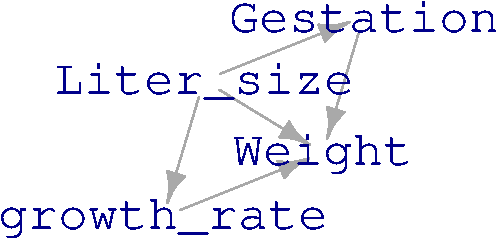
\includegraphics{./Reading-notes-lesson-26_files/figure-pdf/unnamed-chunk-10-1.pdf}

}

\end{figure}

For convenience, the \texttt{model\_plot()} function will do this work
for us, plotting the prediction interval along with the training data.
We can also direct \texttt{model\_plot()} to show the confidence
interval.

\begin{Shaded}
\begin{Highlighting}[]
\DocumentationTok{\#\#\# \#| column: page{-}right}
\FunctionTok{model\_plot}\NormalTok{(Age\_mod, }\AttributeTok{x=}\NormalTok{age, }\AttributeTok{interval=}\StringTok{"prediction"}\NormalTok{, }\AttributeTok{data\_alpha=}\FloatTok{0.05}\NormalTok{)}
\FunctionTok{model\_plot}\NormalTok{(Age\_mod, }\AttributeTok{x=}\NormalTok{age, }\AttributeTok{interval=}\StringTok{"confidence"}\NormalTok{, }\AttributeTok{data\_alpha=}\FloatTok{0.05}\NormalTok{)}
\end{Highlighting}
\end{Shaded}

\begin{figure}[H]

\begin{minipage}[t]{0.50\linewidth}

{\centering 

\raisebox{-\height}{

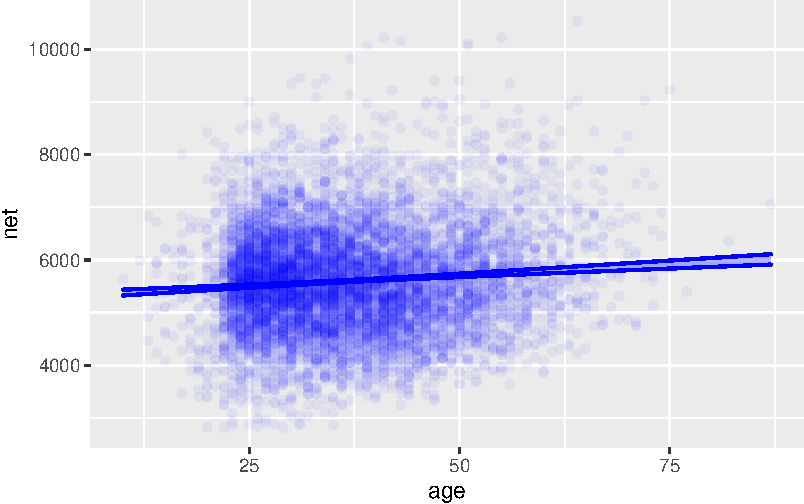
\includegraphics{./Reading-notes-lesson-26_files/figure-pdf/fig-ten-mile-age-confidence-1.pdf}

}

}

\subcaption{\label{fig-ten-mile-age-confidence-1}prediction interval}
\end{minipage}%
%
\begin{minipage}[t]{0.50\linewidth}

{\centering 

\raisebox{-\height}{

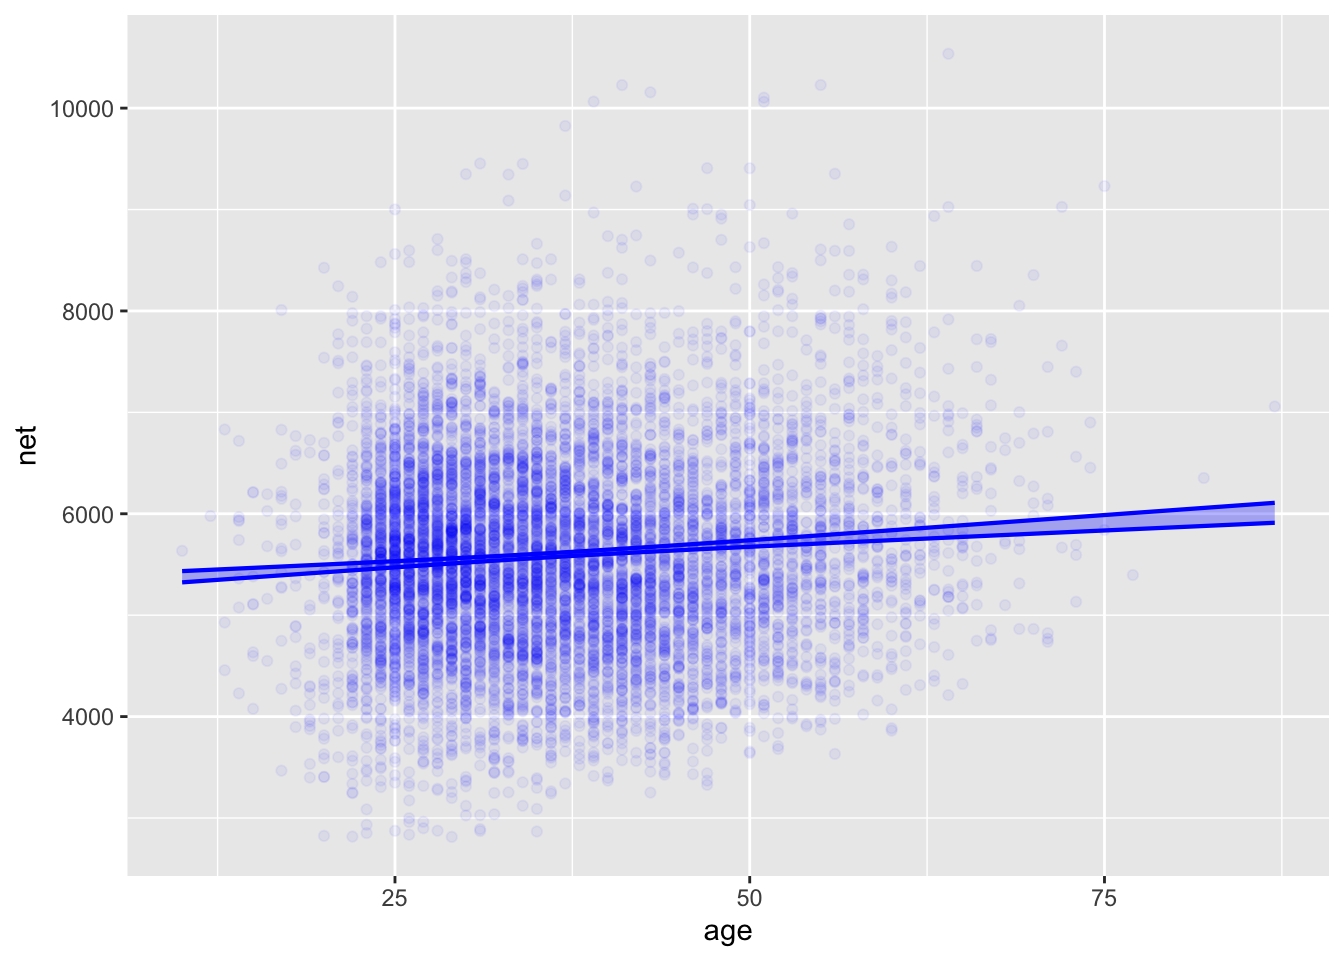
\includegraphics{./Reading-notes-lesson-26_files/figure-pdf/fig-ten-mile-age-confidence-2.pdf}

}

}

\subcaption{\label{fig-ten-mile-age-confidence-2}confidence interval}
\end{minipage}%

\caption{\label{fig-ten-mile-age-confidence}The prediction and
model-function confidence intervals for the model
\texttt{net\ \textasciitilde{}\ age}.}

\end{figure}

Since we are looking at the intervals as a function of an input
variable, what we formerly showed using the ``errorbar'' glyph is now
shown using a ribbon or \textbf{band}.

\end{tcolorbox}

Notice that the prediction interval covers almost all of the data
points. There are hundreds of data points outside the interval, but with
almost 9000 rows in the \texttt{TenMileRace} data frame, an interval
that covers 95\% of the data will have about 450 rows \emph{outside} the
interval.

Such a prediction interval is of little use; it cannot give a precise
prediction about the running time of an individual. The honest
prediction of an individual's outcome needs to reflect the spread of all
the individuals with a similar age.

In contrast, the \emph{confidence} band on the model function is
pleasingly narrow and precise. It covers only a tiny fraction of the raw
data. For this very reason, the confidence interval is
\emph{inappropriate} for presenting a prediction. As always, confidence
intervals only show general trends in the data, not the range of results
for an individual prediction. For instance,
Figure~\ref{fig-ten-mile-age-confidence} shows a clear upward trend in
running time with age. There is no flat or negatively sloping line
compatible with the confidence interval.

To summarize:

\begin{enumerate}
\def\labelenumi{\arabic{enumi}.}
\tightlist
\item
  When making a prediction, report a prediction interval.
\item
  The prediction interval is always larger than the confidence interval
  and is usually \emph{much} larger.
\end{enumerate}

The confidence interval is not for predictions. Use a confidence
interval when looking at an effect size. Graphically, the confidence
interval is to indicate whether there is an overall trend in the model.

\hypertarget{review-of-lessons-19-26}{%
\chapter{Review of Lessons 19-26}\label{review-of-lessons-19-26}}

\begin{tcolorbox}[enhanced jigsaw, colbacktitle=quarto-callout-warning-color!10!white, breakable, opacitybacktitle=0.6, colback=white, left=2mm, arc=.35mm, colframe=quarto-callout-warning-color-frame, coltitle=black, toprule=.15mm, opacityback=0, leftrule=.75mm, bottomtitle=1mm, toptitle=1mm, titlerule=0mm, title=\textcolor{quarto-callout-warning-color}{\faExclamationTriangle}\hspace{0.5em}{Warning}, rightrule=.15mm, bottomrule=.15mm]

I'll put learning challenges here. The class day will be given over to
the QR.

\end{tcolorbox}

\hypertarget{sec-lesson-28}{%
\chapter{Covariates}\label{sec-lesson-28}}

Dr.~Mary Meyer is a statistics professor at Colorado State University.
In 2006, she published
\href{http://jse.amstat.org/v14n1/datasets.meyer.html}{an article}
recounting an episode from family life:

\begin{quote}
\emph{When my daughter was in fourth grade, I took her shopping for
dress shoes. I was disappointed in the quality of girls' shoes at every
store in the mall. The shoes for boys were sturdy and had plenty of room
in the toes. On the other hand, shoes for girls were flimsy, narrow, and
had pointed toes. In spite of the better construction for boys, the
costs of the shoes were similar! For children the same age, boys had
shoes they could run around in, while girls' shoes were clearly for
style and not comfort.}
\end{quote}

\begin{quote}
\emph{Upon complaining about this state of affairs, I was told by sales
representatives in two stores that boys actually had wider feet than
girls, so needed wider shoes. Being very skeptical, I thought I would
test this claim.}
\end{quote}

We will return to Dr.~Meyer's project in a little bit. However, for now,
imagine how this situation might be addressed by someone who still needs
to develop good statistical thinking skills. We will call this imagined
protagonist ``Mr.~Shoebuyer.'' Since the salesmen claimed that girls'
feet are narrower than boys, Mr.~Shoebuyer heads out to measure the
widths of girls' and boys' shoes.

A shoe store provides a convenient place to measure the widths of many
different shoe styles. Mr.~Shoebuyer gets to the shoe store, heads to
the children's section, and starts measuring. For each shoe on display,
he records the shoe width and whether the shoe is for girls or boys.
Here are his data:

\begin{tabular}{l|r}
\hline
sex & width\\
\hline
G & 9.0\\
\hline
G & 8.5\\
\hline
G & 9.0\\
\hline
G & 9.5\\
\hline
B & 8.6\\
\hline
B & 8.4\\
\hline
B & 8.8\\
\hline
B & 9.4\\
\hline
\end{tabular}

Once back home, Mr.~Shoebuyer uses his calculator to find the mean width
of the shoes in each group. His results surprise him:

\begin{longtable}[]{@{}ll@{}}
\toprule()
sex & mean width \\
\midrule()
\endhead
Girls & 9.0 cm \\
Boys & 8.8 cm \\
\bottomrule()
\end{longtable}

Mr.~Shoebuyer happens to be your uncle. He knows you are taking a
statistics course and asks you to check his arithmetic. Putting on a
statistical thinking hat to the effect size of sex on shoe width, you
note the absence of a confidence interval. This omission is easy to fix.

\begin{Shaded}
\begin{Highlighting}[]
\NormalTok{Shoebuyer\_data }\SpecialCharTok{\%\textgreater{}\%} \FunctionTok{lm}\NormalTok{(width }\SpecialCharTok{\textasciitilde{}}\NormalTok{ sex, }\AttributeTok{data=}\NormalTok{.) }\SpecialCharTok{\%\textgreater{}\%} \FunctionTok{conf\_interval}\NormalTok{()}
\end{Highlighting}
\end{Shaded}

\ttfamily 
\begin{tabular}{lrr}
\toprule
term & .lwr & .upr\\
\midrule
(Intercept) & 8.2857603 & 9.3142397\\
sexG & -0.5272448 & 0.9272448\\
\bottomrule
\end{tabular} \normalfont
\bigskip

Your uncle is at the table at Thanksgiving break. ``Sorry, Uncle, but
you don't have nearly enough data to conclude that girls' feet are wider
than boys'.'' Translating the confidence interval into plus-or-minus
format, you point out that the difference between the sexes is
\(0.2 \pm 0.8\) cm. ``You'll need enough data to get that 0.8 margin of
error down to something like 0.2.'' You also point out that there might
be a better place to collect data than a shoe store. ``It's the feet,
not the shoes, that you want to look at.''

Aware of these pitfalls, Dr.~Meyer worked with the third- and
fourth-grade teachers at her daughter's school to collect data. Being a
statistical thinker, she thought about what data would illuminate the
matter before carrying out the data collection. Her data, a sample of
size \(n=39\), are recorded in the \texttt{KidsFeet} data frame.

\begin{Shaded}
\begin{Highlighting}[]
\FunctionTok{lm}\NormalTok{(width }\SpecialCharTok{\textasciitilde{}}\NormalTok{ sex, }\AttributeTok{data =}\NormalTok{ KidsFeet) }\SpecialCharTok{\%\textgreater{}\%} \FunctionTok{conf\_interval}\NormalTok{()}
\end{Highlighting}
\end{Shaded}

\ttfamily 
\begin{tabular}{lrr}
\toprule
term & .lwr & .upr\\
\midrule
(Intercept) & 8.9758882 & 9.4041118\\
sexG & -0.7125476 & -0.0990313\\
\bottomrule
\end{tabular} \normalfont
\bigskip

In plus-or-minus format, this confidence interval is \(-0.4 \pm 0.3\).
Whatever the format, Dr.~Meyer's data provides some evidence that girls'
feet are narrower than boys'.

As a statistical thinker, Dr.~Meyer knows that even though the foot
width is the original quantity of interest, other factors might play a
role in the system. For example, boys' feet might trend longer or
shorter than girls' feet. This possibility should be taken into account
by looking at the effect size of \texttt{sex} on width, holding length
constant. After all, a shoe buyer first tells the salesperson their foot
length (or ``size''); the salesperson then brings shoes of that size to
try on.

\begin{Shaded}
\begin{Highlighting}[]
\FunctionTok{lm}\NormalTok{(width }\SpecialCharTok{\textasciitilde{}}\NormalTok{ sex }\SpecialCharTok{+}\NormalTok{ length, }\AttributeTok{data=}\NormalTok{KidsFeet) }\SpecialCharTok{\%\textgreater{}\%} \FunctionTok{conf\_interval}\NormalTok{()}
\end{Highlighting}
\end{Shaded}

\ttfamily 
\begin{tabular}{lrr}
\toprule
term & .lwr & .upr\\
\midrule
(Intercept) & 1.1048182 & 6.1775184\\
sexG & -0.4947759 & 0.0297408\\
length & 0.1202348 & 0.3218151\\
\bottomrule
\end{tabular} \normalfont
\bigskip

Although \texttt{sex} is the explanatory variable of primary interest to
Dr.~Meyer's question, she knows to include other explanatory variables
that might play a role. Such explanatory variables, not of direct
interest, are called ``\textbf{covariates}.'' Dr.~Meyer's statistical
expertise led her to consider possible covariates \emph{before}
collecting her data and took the trouble of measuring both foot length
and width.

The confidence interval on the \texttt{sexG} coefficient includes zero
when \texttt{length} is taken into account. Dr.~Meyer's little study
provides evidence that even if girls' shoes tend to be narrower than
boys', the feet inside them have about the same shape for both sexes.

\hypertarget{all-other-things-being-equal}{%
\section{All other things being
equal}\label{all-other-things-being-equal}}

The common phrase ``all other things being equal'' is a critical
qualifier in describing relationships. To illustrate: A simple claim in
economics is that a high price for a commodity reduces the demand. For
example, increasing the price of heating fuel will reduce demand as
people turn down thermostats to save money. Nevertheless, the claim can
be considered obvious only with the qualifier \emph{all other things
being equal}. For instance, the fuel price might have increased because
winter weather has increased the demand for heating compared to summer.
Thus, higher prices may be associated with higher demand. Therefore,
increased price may not be associated with lower demand unless holding
other variables, such as weather conditions, constant.

In economics, the Latin equivalent of ``all other things being equal''
is sometimes used: ``\textbf{ceteris paribus}''. So, the economics claim
would be, ``higher prices are associated with lower demand,
\emph{ceteris paribus}.''

Although the phrase ``all other things being equal'' has a logical
simplicity, it is impractical to implement ``all.'' So instead of the
blanket ``all other things,'' it is helpful to consider just ``some
other things'' to be held constant, being explicit about what those
things are. Other phrases along the same lines are ``taking into account
\ldots{}'' and ``controlling for \ldots.'' Those additional variables
that are to be considered are called ``\textbf{covariates}.

\begin{tcolorbox}[enhanced jigsaw, colbacktitle=quarto-callout-note-color!10!white, breakable, opacitybacktitle=0.6, colback=white, left=2mm, arc=.35mm, colframe=quarto-callout-note-color-frame, coltitle=black, toprule=.15mm, opacityback=0, leftrule=.75mm, bottomtitle=1mm, toptitle=1mm, titlerule=0mm, title=\textcolor{quarto-callout-note-color}{\faInfo}\hspace{0.5em}{Example: Covariates and Death}, rightrule=.15mm, bottomrule=.15mm]

This news report appeared in 2007:

\begin{quote}
\textbf{Heart Surgery Drug Carries High Risk, Study Says.} A drug widely
used to prevent excessive bleeding during heart surgery appears to raise
the risk of dying in the five years afterward by nearly 50 percent, an
international study found. The researchers said replacing the
drug---aprotinin, sold by Bayer under the brand name Trasylol---with
other, cheaper drugs for a year would prevent 10,000 deaths worldwide
over the next five years.\\
Bayer said in a statement that the findings are unreliable because
Trasylol tends to be used in more complex operations, and the
researchers' statistical analysis did not fully account for the
complexity of the surgery cases. The study followed 3,876 patients who
had heart bypass surgery at 62 medical centers in 16 nations.
Researchers compared patients who received aprotinin to patients who got
other drugs or no antibleeding drugs. Over five years, 20.8 percent of
the aprotinin patients died, versus 12.7 percent of the patients who
received no antibleeding drug. {[}This is a 64\% increase in the death
rate.{]} When researchers adjusted for other factors, they found that
patients who got Trasylol ran a 48 percent higher risk of dying in the
five years afterward. The other drugs, both cheaper generics, did not
raise the risk of death significantly.
{\marginnote{\begin{footnotesize}``Significant'' has a specialized
meaning in statistical language. It is \emph{not} a synonym for
``important.'' See Lessons 36 through 38\end{footnotesize}}} The study
was not a randomized trial, meaning that it did not randomly assign
patients to get aprotinin or not. In their analysis, the researchers
took into account how sick patients were before surgery, but they
acknowledged that some factors they did not account for may have
contributed to the extra deaths. - Carla K. Johnson, Associated Press, 7
Feb.~2007
\end{quote}

The report involves several variables. Of primary interest is the
relationship between (1) the risk of dying after surgery and (2) the
drug used to prevent excessive bleeding during surgery. Also potentially
important are (3) the complexity of the surgical operation and (4) how
sick the patients were before surgery. Bayer disputes the published
results of the relationship between (1) and (2) holding (4) constant,
saying that it is also essential to hold variable (3) constant.

The total relationship involves a death rate of 20.8 percent of patients
who got aprotinin versus 12.7 percent for the patients taking the
generic drugs: an increase in the death rate by a factor of 1.64.
However, when the researchers looked at a partial relationship (holding
constant patient sickness before the operation), the effect size of
aprotinin on mortality was less: a factor of 1.48. In other words, the
model \texttt{death\ \textasciitilde{}\ aprotinin} shows a 64\% increase
in the death rate, but the model
\texttt{death\ \textasciitilde{}\ aprotinin\ +\ sickness} shows a
slightly smaller increase in death rate: 48\%. The difference between
the two estimates reflects doctors being more likely to give aprotinin
to sicker patients.

The story's last paragraph states that the choice of patients receiving
aprotinin versus the generic drugs was not made at random. Some readers
may find this reassuring. Why in the world would anyone prescribe a drug
at random? The point, however, is to select randomly who gets which drug
\emph{among the patients for whom the drugs would be appropriate}. The
phrase ``randomized trial'' used in the paragraph means specifically an
\emph{experiment} in which one treatment or the other---aprotinin versus
the generic drugs---is assigned at random. The virtues of experiment and
the vital role of random assignment are detailed in
Lesson~\ref{sec-lesson-32}.

\end{tcolorbox}

\hypertarget{letting-things-change-as-they-will}{%
\section{Letting things change as they
will}\label{letting-things-change-as-they-will}}

Using covariates in models enables the relationship between a response
and an explanatory variable to be described \emph{ceteris paribus}, that
is, ``all other things being equal.'' Another phrase used in news
stories is ``after adjusting for \ldots.'' This is appropriate since the
\emph{all} in ``all other things'' is, in reality, refers only to those
particular factors used as the covariates in the model. So, Dr.~Meyer's
foot width results might be stated in everyday language as, ``After
adjusting for foot width, she found no difference in the widths of
girls' and boys' feet.''

Not including covariates in a model amounts to ``letting other things
change as they will.'' In Latin, this is ``\emph{mutatis mutandis}.'' In
the foot-width example, the model \texttt{width\ \textasciitilde{}\ sex}
looks at the differences in foot width for the two sexes. However, sex
is not the only thing associated with foot width. The model
\texttt{width\ \textasciitilde{}\ sex} ignores all other factors than
sex; it compares boys and girls \emph{mutatis mutandis}, that is,
letting other things change as they will. In this case, comparing boys
and girls involves not just the possible differences in foot width but
also the differences in other factors such as foot length and body
weight.

\begin{tcolorbox}[enhanced jigsaw, colbacktitle=quarto-callout-note-color!10!white, breakable, opacitybacktitle=0.6, colback=white, left=2mm, arc=.35mm, colframe=quarto-callout-note-color-frame, coltitle=black, toprule=.15mm, opacityback=0, leftrule=.75mm, bottomtitle=1mm, toptitle=1mm, titlerule=0mm, title=\textcolor{quarto-callout-note-color}{\faInfo}\hspace{0.5em}{Example: One change can bring another}, rightrule=.15mm, bottomrule=.15mm]

I was once involved in a budget committee that recommended employee
health benefits for the college where I worked. At the time, college
employees who belonged to the college's insurance plan received a
generous subsidy for their health insurance costs. Employees who did not
belong to the plan received no subsidy but were given a modest monthly
cash payment. After the stock market crashed in 2000, the college needed
to cut budgets. One proposal called for eliminating the cash payment to
employees who did not belong to the insurance plan. Proponents of the
plan claimed that this would save money without reducing health
benefits. I argued that this claim was an ``all other things being
equal'' analysis: how expenditures would change assuming the number of
people belonging to the insurance plan remained constant. In reality,
however, the policy change would play out \emph{mutatis matandis}; the
loss of the cash payment would cause some employees, who currently
received health benefits through their spouse's health plan, to switch
to the college's health plan. That is what happened, contributing to an
overall increase in healthcare expenses.

\end{tcolorbox}

\begin{tcolorbox}[enhanced jigsaw, colbacktitle=quarto-callout-note-color!10!white, breakable, opacitybacktitle=0.6, colback=white, left=2mm, arc=.35mm, colframe=quarto-callout-note-color-frame, coltitle=black, toprule=.15mm, opacityback=0, leftrule=.75mm, bottomtitle=1mm, toptitle=1mm, titlerule=0mm, title=\textcolor{quarto-callout-note-color}{\faInfo}\hspace{0.5em}{Example: Spending and student performance}, rightrule=.15mm, bottomrule=.15mm]

To illustrate how covariates set context, consider an issue of interest
to public policy-makers in many societies: How much money to spend on
children's education? State lawmakers in the US are understandably
concerned with the quality of public education provided. However, they
also have other concerns and constraints and constituencies who give
budget priority to other matters.

In evaluating their various trade-offs, lawmakers could benefit by
knowing how increased educational spending will shape educational
outcomes. What can available data tell us? Unfortunately, there are
various political constraints that work against states adopting and
publishing data on a standard, genuine measure of educational outcome.
Instead, we have high-school graduation rates, student grades, and other
non-standardized data. These data might have some meaning but can also
reflect system gaming by administrators and teachers, for which there is
little systematic data.

Although imperfect, college admissions tests such as the ACT and SAT
provide consistent data between states. For example,
Figure~\ref{fig-sat-1} shows the average SAT score in 2010 in each state
versus expenditures per pupil in public elementary and secondary
schools. Layered on top of the data is a flexible linear model (and its
confidence band) of SAT score versus expenditure.

The overall impression given by the model is that the relationship is
negative, with lower expenditures corresponding to higher SAT scores.
However, the confidence band is broad; it is possible to find a smooth
path with almost zero slope through the confidence band. Either way,
this graph does not support the conventional wisdom that higher spending
produces better school outcomes.

\begin{figure}[H]

{\centering 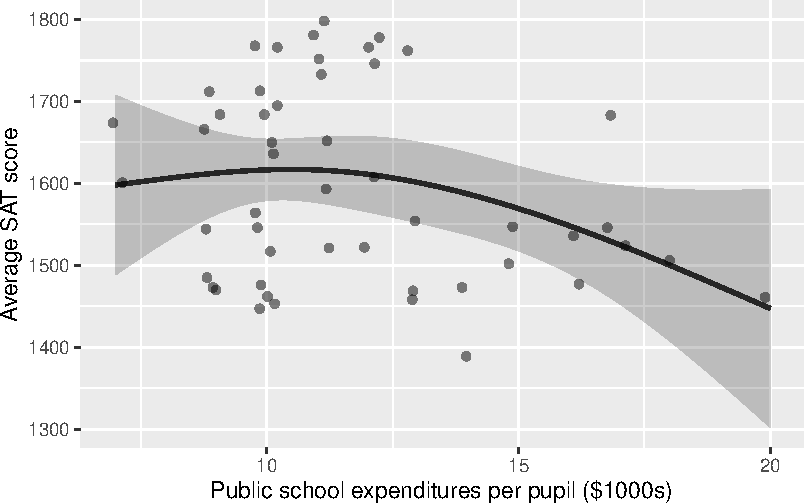
\includegraphics{./Reading-notes-lesson-28_files/figure-pdf/fig-sat-1-1.pdf}

}

\caption{\label{fig-sat-1}State by state data (from 2010) on average SAT
college admissions test scores and expenditures for public education.}

\end{figure}

Of course, other factors play a role in shaping education outcomes: for
instance, poverty levels, parental education, and how the educational
money is spent (higher pay for teachers or smaller class sizes?
administrative bloat?).

At first glance, it is tempting to ignore these additional factors. For
instance, we may not have data on them. Moreover, as our interest is in
understanding the relationship between expenditures and education
outcomes, we are not directly concerned with the additional factors.
However, the lack of direct concern does not imply that we should ignore
the factors but that we should do what we can to ``hold them constant''.

To illustrate, consider the fraction of eligible students (those in
their last year of high school) who take the college admission test.
This fraction varies widely from state to state. In a poor state where
few students go to college, the fraction can be tiny (Alabama 8\%,
Arkansas 5\%, Mississippi 4\%, Louisiana 8\%). In some other states, the
large majority of students take the SAT (Maine 93\%, Massachusetts 89\%,
New York 89\%). In states with low SAT participation rates, the students
who take the test tend to be those applying to schools with competitive
admissions. Such strong students will get high scores. In contrast, the
scores in states with high participation rates reflect both strong and
weak students. Consequently, the scores will be lower on average than in
the low-participation states.

Putting the relationship between expenditure and SAT scores in the
context of the fraction taking the SAT is accomplished with the model
\texttt{SAT\ \textasciitilde{}\ expenditure\ +\ fraction} rather than
just \texttt{SAT\ \textasciitilde{}\ expenditure}.
Figure~\ref{fig-sat-3} shows a model with \texttt{fraction} as a
covariate.

\begin{figure}[H]

{\centering 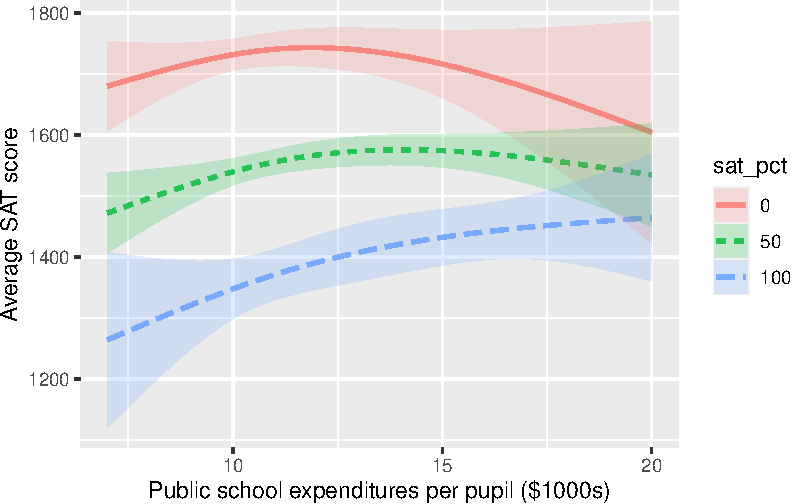
\includegraphics{./Reading-notes-lesson-28_files/figure-pdf/fig-sat-3-1.pdf}

}

\caption{\label{fig-sat-3}The model of SAT score versus expenditures,
including as a covariate the fraction of eligible students in the state
who take the SAT.}

\end{figure}

Note that the effect size of spending on SAT scores is positive when the
expenditure level is less than \$10,000 per pupil. Notice as well that
when the fraction taking the SAT is tiny, the average scores do not
depend on expenditure. This flat relationship suggests that, among elite
students, state expenditure does not make a discernible difference.
Perhaps the college-bound students in such states have other educational
resources to draw on.

The relationship shown in Figure~\ref{fig-sat-1} is genuine. However, so
is the very different relationship seen in Figure~\ref{fig-sat-3}. How
can the same data be consistent with two utterly different displays? The
answer, perhaps unexpectedly, has to do with the connections among the
explanatory variables. Whatever the relationship between an individual
explanatory variable and the response variable, the \emph{appearance} of
that relationship will depend on which covariates the modeler chooses to
include.

\end{tcolorbox}

\hypertarget{sec-lesson-29}{%
\chapter{Covariates eat variance}\label{sec-lesson-29}}

In Lesson~\ref{sec-lesson-28}, we introduced covariates to set the
relationship between an explanatory variable and the response variable
in the correct context. In Lesson 30, we will return to this
context-setting role to show that the appropriate choice of covariates
to include in a model depends on the modeler's opinion about the
relevant structure of a DAG. Here, we will treat covariates as commodity
items to show a surprising property of models. This property is a boon
to the modeler, helping to enable sound decisions about whether to
include any given covariate. However, it is also a pitfall lieing in
wait for the wishful thinker.

\hypertarget{how-much-variation-is-explained}{%
\section{How much variation is
explained}\label{how-much-variation-is-explained}}

We start by returning to the definition of statistical thinking
introduced at the start of these Lessons:

\begin{quote}
\emph{Statistic thinking is the explanation or description of variation}
in the context of \emph{what remains unexplained or undescribed.}
\end{quote}

In this Lesson, we will work with a straightforward measure of ``what
remains unexplained or undescribed.'' The fitted model values represent
the explained part of the variation. The residuals are what is left
over, the difference between the actual values of the response variable
and the fitted model values.

As a reminder, we will construct a simple model of the list price of
books as a function of the number of pages and whether the book is a
paperback or hardcover.\footnote{If you seek to duplicate the results
  presented in this chapter, please note that we have deleted six rows
  from `amazon\_books because the rows are either duplicates or have one
  of the variables missing. The deleted rows are 62, 103, 205, 211, 242,
  and 303.}

\begin{Shaded}
\begin{Highlighting}[]
\NormalTok{Price\_model }\OtherTok{\textless{}{-}} \FunctionTok{lm}\NormalTok{(list\_price }\SpecialCharTok{\textasciitilde{}}\NormalTok{ num\_pages }\SpecialCharTok{+}\NormalTok{ hard\_paper, }
                  \AttributeTok{data =}\NormalTok{ amazon\_books)}
\end{Highlighting}
\end{Shaded}

The \texttt{model\_eval()} function can extract the fitted model values
and the residuals from the model. We show just a few rows here, but we
will use the entire report from \texttt{model\_eval()}. Remember that
when \texttt{model\_eval()} is not given input values, it uses the model
\emph{training} data as input.

\begin{Shaded}
\begin{Highlighting}[]
\NormalTok{Results }\OtherTok{\textless{}{-}} \FunctionTok{model\_eval}\NormalTok{(Price\_model)}
\end{Highlighting}
\end{Shaded}

\begin{verbatim}
Using training data as input to model_eval().
\end{verbatim}

\ttfamily 
\begin{tabular}{rrlrrrr}
\toprule
.response & num\_pages & hard\_paper & .output & .resid & .lwr & .upr\\
\midrule
12.95 & 304 & P & 16.60 & -3.65 & -10.73 & 43.94\\
15.00 & 273 & P & 15.98 & -0.98 & -11.36 & 43.32\\
1.50 & 96 & P & 12.45 & -10.95 & -14.97 & 39.88\\
15.99 & 672 & P & 23.95 & -7.96 & -3.57 & 51.47\\
30.50 & 720 & P & 24.91 & 5.59 & -2.67 & 52.49\\
\addlinespace
28.95 & 460 & H & 24.57 & 4.38 & -2.89 & 52.03\\
\bottomrule
\end{tabular} \normalfont
\bigskip

The first book in the training data is a 304-page paperback with a list
price of \$12.95. The fitted model value for that book is \$16.60.
(Ordinarily, we refer to the output of the model function simply as the
``output'' or the ``model output.'' However, the output of the model
function, when applied to rows from the \emph{training} data also called
the \emph{fitted model value}.)

At \$16.60, the fitted model value is \$3.65 \emph{higher} than the list
price. This difference is the residual for that book, the sign
reflecting the definition
\[\text{residual} \equiv \text{response value} - \text{fitted model value}\ .\]
When the residual is small in magnitude, the fitted model value is close
to the response value. Conversely, a large residual means the model was
way off target for that book.

The standard measure of the typical size of a residual is the standard
deviation or, equivalently, the variance.

\begin{Shaded}
\begin{Highlighting}[]
\NormalTok{Results }\SpecialCharTok{\%\textgreater{}\%} \FunctionTok{summarize}\NormalTok{(}\AttributeTok{se\_resids =} \FunctionTok{sd}\NormalTok{(.resid), }\AttributeTok{v\_resids=}\FunctionTok{var}\NormalTok{(.resid))}
\end{Highlighting}
\end{Shaded}

\ttfamily 
\begin{tabular}{rr}
\toprule
se\_resids & v\_resids\\
\midrule
13.81885 & 190.9606\\
\bottomrule
\end{tabular} \normalfont
\bigskip

As always, the standard deviation is easier to read because it has
sensible units, in this case, dollars. On the other hand, the variance
has strange units (square dollars) because it is the square of the
standard deviation. We will use the variance for measuring the typical
size of a residual for the reasons described in
Lesson~\ref{sec-lesson-20}; variances add nicely in a manner analogous
to the Pythagorean Theorem.

A simple measure of how much of the variation in the response variable
remains \emph{unexplained} is the ratio of the variance of the residuals
and the variance of the response variable.

\begin{Shaded}
\begin{Highlighting}[]
\NormalTok{Results }\SpecialCharTok{\%\textgreater{}\%} \FunctionTok{summarize}\NormalTok{(}\AttributeTok{unexplained\_fraction =} \FunctionTok{var}\NormalTok{(.resid)}\SpecialCharTok{/}\FunctionTok{var}\NormalTok{(.response))}
\end{Highlighting}
\end{Shaded}

\ttfamily 
\begin{tabular}{r}
\toprule
unexplained\_fraction\\
\midrule
0.9246907\\
\bottomrule
\end{tabular} \normalfont
\bigskip

More than 90\% of the variation remains unexplained by the
\texttt{Price\_model}! This high fraction of unexplained variance
suggests the model has little to tell us. In the spirit of putting a
positive spin on things, statisticians typically work with the
complement of the unexplained fraction. Since the unexplained fraction
is 92.5\%, the complement is 7.5\%. This number is written
R\textsuperscript{2} and pronounced ``R-squared.'' (It also has a formal
name: the ``coefficient of determination.'' In
Lesson~\ref{sec-lesson-30}, we will meet the inventor of the coefficient
of determination, Sewall Wright, who is an early hero of causal
reasoning.)

R\textsuperscript{2} is such a widely used summary of how the
explanatory variables account for the response variable that a software
extractor calculates it and some related values.

\begin{Shaded}
\begin{Highlighting}[]
\NormalTok{Price\_model }\SpecialCharTok{\%\textgreater{}\%} \FunctionTok{R2}\NormalTok{()}
\end{Highlighting}
\end{Shaded}

\ttfamily 
\begin{tabular}{rrrrr}
\toprule
n & k & Rsquared & F & adjR2\\
\midrule
317 & 2 & 0.0753093 & 12.78651 & 0.0694196\\
\bottomrule
\end{tabular} \normalfont
\bigskip

Many modelers act as if their goal is to build a model that makes
R\textsuperscript{2} as big as possible. Their thinking is that large
R\textsuperscript{2} means that the explanatory variables account for
much of the response variable's variance. Unfortunately, it is a naive
goal. Instead, always focus on the model's suitability for the purpose
at hand. Often, shooting for a large R\textsuperscript{2} imposes costs
that can undermine the purpose for the model. Furthermore, even models
with the largest possible R\textsuperscript{2} sometimes have nothing to
say about the response variable.

\hypertarget{getting-to-1}{%
\section{Getting to 1}\label{getting-to-1}}

R\textsuperscript{2} can range from zero to one. Zero means that the
model accounts for \emph{none} of the variation in the response
variable. We can construct such a model quickly enough:
\texttt{list\_price\ \textasciitilde{}\ 1} has no explanatory variables
and, therefore, no ability to distinguish one book from another.

\begin{Shaded}
\begin{Highlighting}[]
\NormalTok{Null\_model }\OtherTok{\textless{}{-}} \FunctionTok{lm}\NormalTok{(list\_price }\SpecialCharTok{\textasciitilde{}} \DecValTok{1}\NormalTok{, }\AttributeTok{data =}\NormalTok{ amazon\_books)}
\NormalTok{Null\_model }\SpecialCharTok{\%\textgreater{}\%} \FunctionTok{R2}\NormalTok{()}
\end{Highlighting}
\end{Shaded}

\ttfamily 
\begin{tabular}{rrrrr}
\toprule
n & k & Rsquared & F & adjR2\\
\midrule
319 & 0 & 0 & NaN & 0\\
\bottomrule
\end{tabular} \normalfont
\bigskip

We are using the word ``null'' to name this model. ``Null'' is part of
the statistics tradition. The dictionary definition of ``null'' is
``having or associated with the value zero'' or ``lacking distinctive
qualities; having no positive substance or content.''\footnote{Source:
  \href{https://languages.oup.com/dictionaries/}{Oxford Languages}}

In the null model, the fitted model values are all the same; all the
variation is in the residuals.

\begin{Shaded}
\begin{Highlighting}[]
\NormalTok{Null\_model }\SpecialCharTok{\%\textgreater{}\%} \FunctionTok{model\_eval}\NormalTok{()}
\end{Highlighting}
\end{Shaded}

\begin{verbatim}
Using training data as input to model_eval().
\end{verbatim}

\begin{verbatim}
Using training data as input to model_eval().
\end{verbatim}

\begin{tabular}{r|r|r|r|r}
\hline
.response & .output & .resid & .lwr & .upr\\
\hline
12.95 & 18.6 & -5.65 & -9.69 & 46.89\\
\hline
15.00 & 18.6 & -3.60 & -9.69 & 46.89\\
\hline
1.50 & 18.6 & -17.10 & -9.69 & 46.89\\
\hline
15.99 & 18.6 & -2.61 & -9.69 & 46.89\\
\hline
30.50 & 18.6 & 11.90 & -9.69 & 46.89\\
\hline
28.95 & 18.6 & 10.35 & -9.69 & 46.89\\
\hline
\end{tabular}

At the other extreme, where R\textsuperscript{2} = 1, the explanatory
variables account for every bit of variation in the response variable.
We can try various combinations of explanatory variables to see if we
can accomplish this. For example, \texttt{publisher} explains 67\% of
the variation in list price.

\begin{Shaded}
\begin{Highlighting}[]
\FunctionTok{lm}\NormalTok{(list\_price }\SpecialCharTok{\textasciitilde{}}\NormalTok{ publisher, }\AttributeTok{data =}\NormalTok{ amazon\_books) }\SpecialCharTok{\%\textgreater{}\%} \FunctionTok{R2}\NormalTok{()}
\end{Highlighting}
\end{Shaded}

\ttfamily 
\begin{tabular}{rrrrr}
\toprule
n & k & Rsquared & F & adjR2\\
\midrule
319 & 158 & 0.6749786 & 2.103008 & 0.3540199\\
\bottomrule
\end{tabular} \normalfont
\bigskip

We can also check whether \texttt{author} has anything to say about the
list price.

\begin{Shaded}
\begin{Highlighting}[]
\FunctionTok{lm}\NormalTok{(list\_price }\SpecialCharTok{\textasciitilde{}}\NormalTok{ author, }\AttributeTok{data =}\NormalTok{ amazon\_books) }\SpecialCharTok{\%\textgreater{}\%} \FunctionTok{R2}\NormalTok{()}
\end{Highlighting}
\end{Shaded}

\ttfamily 
\begin{tabular}{rrrrr}
\toprule
n & k & Rsquared & F & adjR2\\
\midrule
319 & 250 & 0.9434046 & 4.534044 & 0.7353333\\
\bottomrule
\end{tabular} \normalfont
\bigskip

Incredible! How about if we use \emph{both} \texttt{publisher} and
\texttt{author} as explanatory variables? We get very close to
R\textsuperscript{2} = 1.

\begin{Shaded}
\begin{Highlighting}[]
\FunctionTok{lm}\NormalTok{(list\_price }\SpecialCharTok{\textasciitilde{}}\NormalTok{ publisher }\SpecialCharTok{+}\NormalTok{ author, }\AttributeTok{data =}\NormalTok{ amazon\_books) }\SpecialCharTok{\%\textgreater{}\%}
  \FunctionTok{R2}\NormalTok{()}
\end{Highlighting}
\end{Shaded}

\ttfamily 
\begin{tabular}{rrrrr}
\toprule
n & k & Rsquared & F & adjR2\\
\midrule
319 & 281 & 0.9821609 & 7.249441 & 0.84668\\
\bottomrule
\end{tabular} \normalfont
\bigskip

The modeler discovering this tremendous explanatory power of
\texttt{publisher} and \texttt{author} can be forgiven for thinking he
or she has found a meaningful explanation. But, unfortunately, the high
R\textsuperscript{2} is an illusion in this case.

To see why, consider another possible explanatory variable, the
International Standard Book Number (ISBN). The ISBN is a ten- or
thirteen-digit number that marks each book with a unique number.

\begin{marginfigure}

{\centering 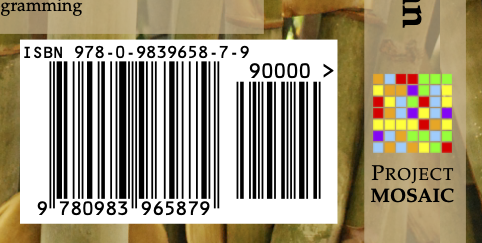
\includegraphics[width=1.61in,height=\textheight]{./www/SM2-ISBN.png}

}

\caption{\label{fig-isbn-sm2}The ISBN number from one of the Project
MOSAIC textbooks.}

\end{marginfigure}

There is a system behind ISBNs, but despite the ``N'' standing for
``number,'' an ISBN is a character string or word (written using only
digits). Consequently, the \texttt{isbn\_10} variable in
\texttt{amazon\_books}is categorical.

\begin{Shaded}
\begin{Highlighting}[]
\NormalTok{ISBN\_model }\OtherTok{\textless{}{-}} \FunctionTok{lm}\NormalTok{(list\_price }\SpecialCharTok{\textasciitilde{}}\NormalTok{ isbn\_10, }\AttributeTok{data =}\NormalTok{ amazon\_books)}
\NormalTok{ISBN\_model }\SpecialCharTok{\%\textgreater{}\%} \FunctionTok{R2}\NormalTok{()}
\end{Highlighting}
\end{Shaded}

\ttfamily 
\begin{tabular}{rrrrr}
\toprule
n & k & Rsquared & F & adjR2\\
\midrule
319 & 318 & 1 & NaN & NaN\\
\bottomrule
\end{tabular} \normalfont
\bigskip

The \texttt{isbn\_10} explains all variation in the list price!

Given that the ISBN is, as we have said, an arbitrary sequence of
characters, why does it do such a good job of accounting for the list
price? The answer lies not in the content of the ISBN but in another
fact: each book has a unique ISBN. As well, each book has a single
price. So the ISBN identifies the price of each book. Cleverness is not
involved; the list price could be anything, and the ISBN would still
identify it precisely. The model coefficients store the whole set of
ISBNs and the corresponding set of list prices.

We can substantiate the claim just made---that the list price could be
anything at all---by synthesizing a data frame with random list prices:

\begin{Shaded}
\begin{Highlighting}[]
\NormalTok{amazon\_books }\SpecialCharTok{\%\textgreater{}\%} 
  \FunctionTok{mutate}\NormalTok{(}\AttributeTok{random\_list\_price =} \FunctionTok{rnorm}\NormalTok{(}\FunctionTok{nrow}\NormalTok{(.))) }\SpecialCharTok{\%\textgreater{}\%}
  \FunctionTok{lm}\NormalTok{(random\_list\_price }\SpecialCharTok{\textasciitilde{}}\NormalTok{ isbn\_10, }\AttributeTok{data =}\NormalTok{ .) }\SpecialCharTok{\%\textgreater{}\%}
  \FunctionTok{R2}\NormalTok{()}
\end{Highlighting}
\end{Shaded}

\ttfamily 
\begin{tabular}{rrrrr}
\toprule
n & k & Rsquared & F & adjR2\\
\midrule
319 & 318 & 1 & NaN & NaN\\
\bottomrule
\end{tabular} \normalfont
\bigskip

Similar randomization can be accomplished by \emph{shuffling} the
\texttt{isbn\_10} column of the data frame so that each ISBN points to a
random book. Of course, such shuffling destroys the link between the
ISBN and the list price. Even so, the R\textsuperscript{2} remains high.

\begin{Shaded}
\begin{Highlighting}[]
\FunctionTok{lm}\NormalTok{(list\_price }\SpecialCharTok{\textasciitilde{}} \FunctionTok{shuffle}\NormalTok{(isbn\_10), }\AttributeTok{data=}\NormalTok{amazon\_books) }\SpecialCharTok{\%\textgreater{}\%} \FunctionTok{R2}\NormalTok{()}
\end{Highlighting}
\end{Shaded}

\ttfamily 
\begin{tabular}{rrrrr}
\toprule
n & k & Rsquared & F & adjR2\\
\midrule
319 & 318 & 1 & NaN & NaN\\
\bottomrule
\end{tabular} \normalfont
\bigskip

\begin{Shaded}
\begin{Highlighting}[]
\FunctionTok{lm}\NormalTok{(}\FunctionTok{shuffle}\NormalTok{(list\_price) }\SpecialCharTok{\textasciitilde{}}\NormalTok{ isbn\_10, }\AttributeTok{data=}\NormalTok{amazon\_books) }\SpecialCharTok{\%\textgreater{}\%} \FunctionTok{R2}\NormalTok{()}
\end{Highlighting}
\end{Shaded}

\ttfamily 
\begin{tabular}{rrrrr}
\toprule
n & k & Rsquared & F & adjR2\\
\midrule
319 & 318 & 1 & NaN & NaN\\
\bottomrule
\end{tabular} \normalfont
\bigskip

Statistical nomenclature is obscure here. So we will make up a name for
such incidental alignment with no true explanatory power: the
``\textbf{ISBN-effect}.''

Statistical thinkers know to be aware of situations where categorical
variables have many levels and check whether the ISBN effect is in play.

\hypertarget{the-isbn-effect-as-a-benchmark}{%
\section{The ISBN effect as a
benchmark}\label{the-isbn-effect-as-a-benchmark}}

Shuffling an explanatory variable (while keeping the response variable
in the original order) voids any possible explanatory connection between
the two. An R\textsuperscript{2}=0, as we get from any model of the form
\texttt{y\ \textasciitilde{}\ 1}, signals that the \texttt{1} cannot
account for any variation. However, this does not mean shuffling will
lead to R\textsuperscript{2} = 0. Instead, there is a systematic
relationship between the number of model coefficients associated with
the shuffled variable, the sample size \(n\), and R\textsuperscript{2}.

We can demonstrate this relationship by conducting many trials of
modeling the \texttt{list\_price} with a shuffled explanatory variable:
either \texttt{publisher}, \texttt{author}, or \texttt{isbn\_10}.

\begin{tcolorbox}[enhanced jigsaw, colbacktitle=quarto-callout-warning-color!10!white, breakable, opacitybacktitle=0.6, colback=white, left=2mm, arc=.35mm, colframe=quarto-callout-warning-color-frame, coltitle=black, toprule=.15mm, opacityback=0, leftrule=.75mm, bottomtitle=1mm, toptitle=1mm, titlerule=0mm, title=\textcolor{quarto-callout-warning-color}{\faExclamationTriangle}\hspace{0.5em}{Demonstration: Counting coefficients}, rightrule=.15mm, bottomrule=.15mm]

The \texttt{amazon\_books} data frame has \(n=319\) rows.\footnote{The
  data frame in the \texttt{moderndive} package has six additional rows,
  which we have deleted as duplicates or because of missing data.} In
the next computing chunk, we fit the model
\texttt{list\_price\ \textasciitilde{}\ publisher} and collect the
coefficients for counting:

\begin{Shaded}
\begin{Highlighting}[]
\NormalTok{Publisher\_model }\OtherTok{\textless{}{-}} \FunctionTok{lm}\NormalTok{(list\_price }\SpecialCharTok{\textasciitilde{}} \FunctionTok{shuffle}\NormalTok{(publisher),}
                      \AttributeTok{data=}\NormalTok{amazon\_books)}
\NormalTok{Coefficients }\OtherTok{\textless{}{-}}\NormalTok{ Publisher\_model }\SpecialCharTok{\%\textgreater{}\%} \FunctionTok{coef}\NormalTok{() }\SpecialCharTok{\%\textgreater{}\%} \FunctionTok{data.frame}\NormalTok{()}
\FunctionTok{nrow}\NormalTok{(Coefficients)}
\end{Highlighting}
\end{Shaded}

\begin{verbatim}
[1] 159
\end{verbatim}

There are 161 coefficients in the model, the first one being the
``Intercept.'' We will show only the first few.

\begin{Shaded}
\begin{Highlighting}[]
\NormalTok{Coefficients }\SpecialCharTok{\%\textgreater{}\%} \FunctionTok{head}\NormalTok{()}
\end{Highlighting}
\end{Shaded}

\ttfamily 
\begin{tabular}{lr}
\toprule
  & value\\
\midrule
(Intercept) & 14.95\\
shuffle(publisher)Adams Media & 0.05\\
shuffle(publisher)Akashic Books & 13.00\\
shuffle(publisher)Aladdin & 15.05\\
shuffle(publisher)Albert Whitman \& Company & -0.95\\
\addlinespace
shuffle(publisher)Alfred A. Knopf & 0.05\\
\bottomrule
\end{tabular} \normalfont
\bigskip

Altogether, there are \(k=160\) coefficients relating to
\texttt{shuffle(publisher)}.

\end{tcolorbox}

The theory relating R\textsuperscript{2} to the number of coefficients
associated is straightforward for shuffled explanatory variables:
R\textsuperscript{2} will be random with mean value \(\frac{k}{n-1}\).

\begin{tcolorbox}[enhanced jigsaw, colbacktitle=quarto-callout-warning-color!10!white, breakable, opacitybacktitle=0.6, colback=white, left=2mm, arc=.35mm, colframe=quarto-callout-warning-color-frame, coltitle=black, toprule=.15mm, opacityback=0, leftrule=.75mm, bottomtitle=1mm, toptitle=1mm, titlerule=0mm, title=\textcolor{quarto-callout-warning-color}{\faExclamationTriangle}\hspace{0.5em}{Demonstration: The mean R\textsuperscript{2} across many trials}, rightrule=.15mm, bottomrule=.15mm]

For the \texttt{shuffle(publisher)} model, the theoretical mean across
many trials will be R\textsuperscript{2} = 158/324 = 0.49. The
demonstration below confirms this using 100 trials:

\begin{Shaded}
\begin{Highlighting}[]
\NormalTok{Pub\_trials }\OtherTok{\textless{}{-}} \FunctionTok{do}\NormalTok{(}\DecValTok{100}\NormalTok{) }\SpecialCharTok{*}\NormalTok{ \{}
  \FunctionTok{lm}\NormalTok{(list\_price }\SpecialCharTok{\textasciitilde{}} \FunctionTok{shuffle}\NormalTok{(publisher), }\AttributeTok{data=}\NormalTok{amazon\_books) }\SpecialCharTok{\%\textgreater{}\%}
    \FunctionTok{R2}\NormalTok{()}
\NormalTok{\}}
\NormalTok{Pub\_trials }\SpecialCharTok{\%\textgreater{}\%} \FunctionTok{summarize}\NormalTok{(}\AttributeTok{meanR2 =} \FunctionTok{mean}\NormalTok{(Rsquared))}
\end{Highlighting}
\end{Shaded}

\ttfamily 
\begin{tabular}{r}
\toprule
meanR2\\
\midrule
0.4955462\\
\bottomrule
\end{tabular} \normalfont
\bigskip

\end{tcolorbox}

\begin{marginfigure}

{\centering 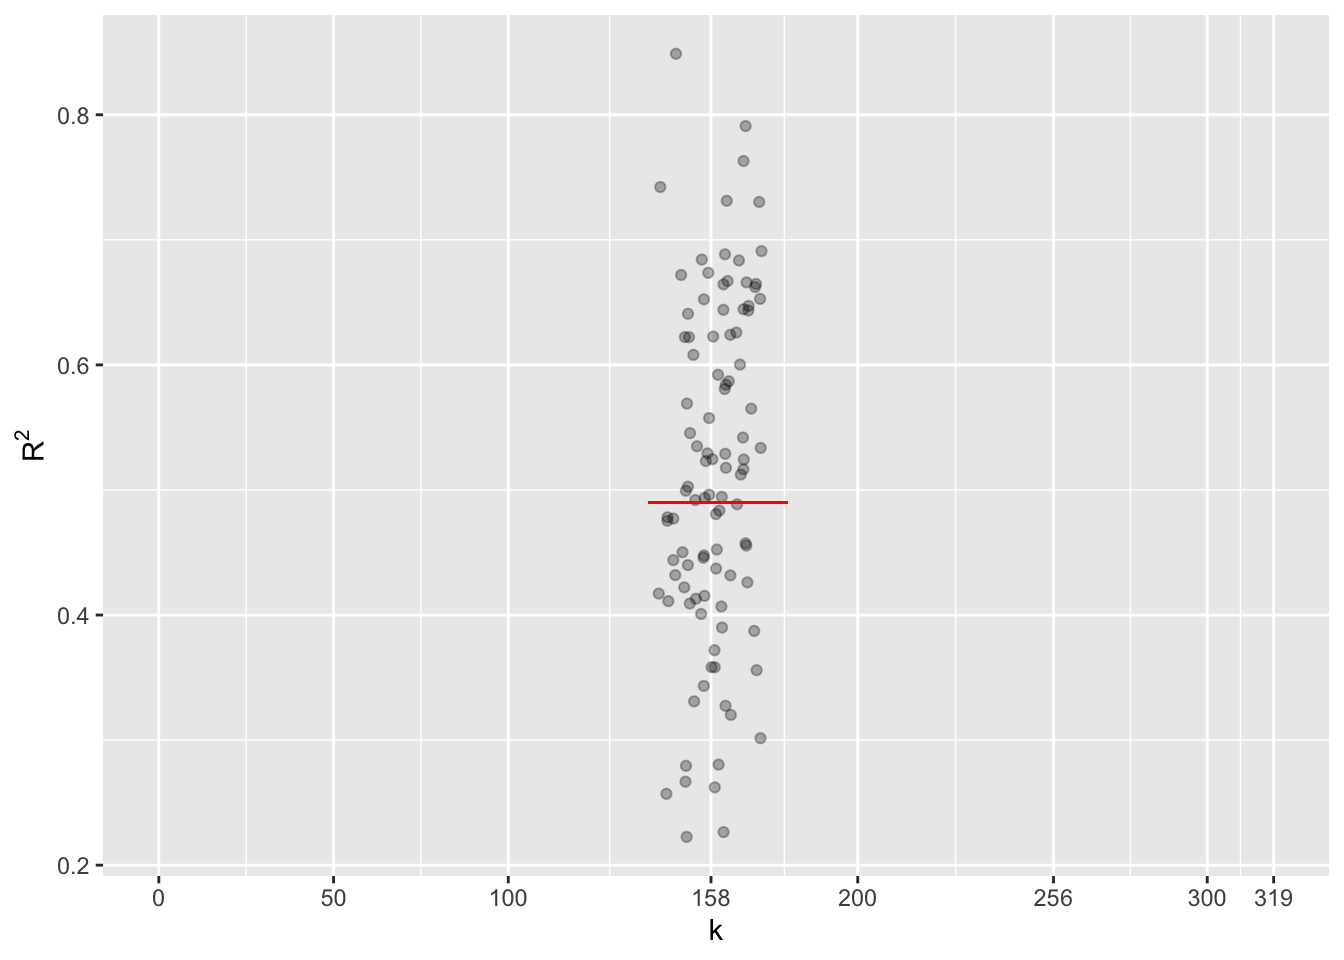
\includegraphics{./Reading-notes-lesson-29_files/figure-pdf/fig-pub-trials-1.pdf}

}

\caption{\label{fig-pub-trials}100 trials of R\textsuperscript{2} from
\texttt{list\_price\ \textasciitilde{}\ shuffled(publisher)}. The
theoretical value \(k/n=160/324=0.49\) is marked in red.}

\end{marginfigure}

We can carry out similar trials for the models
\texttt{list\_price\ \textasciitilde{}\ shuffle(author)} and
\texttt{list\_price\ \textasciitilde{}\ shuffle(isbn\_10)}, which have
\(k=251\) and \(k=319\) respectively.

\begin{figure}

{\centering 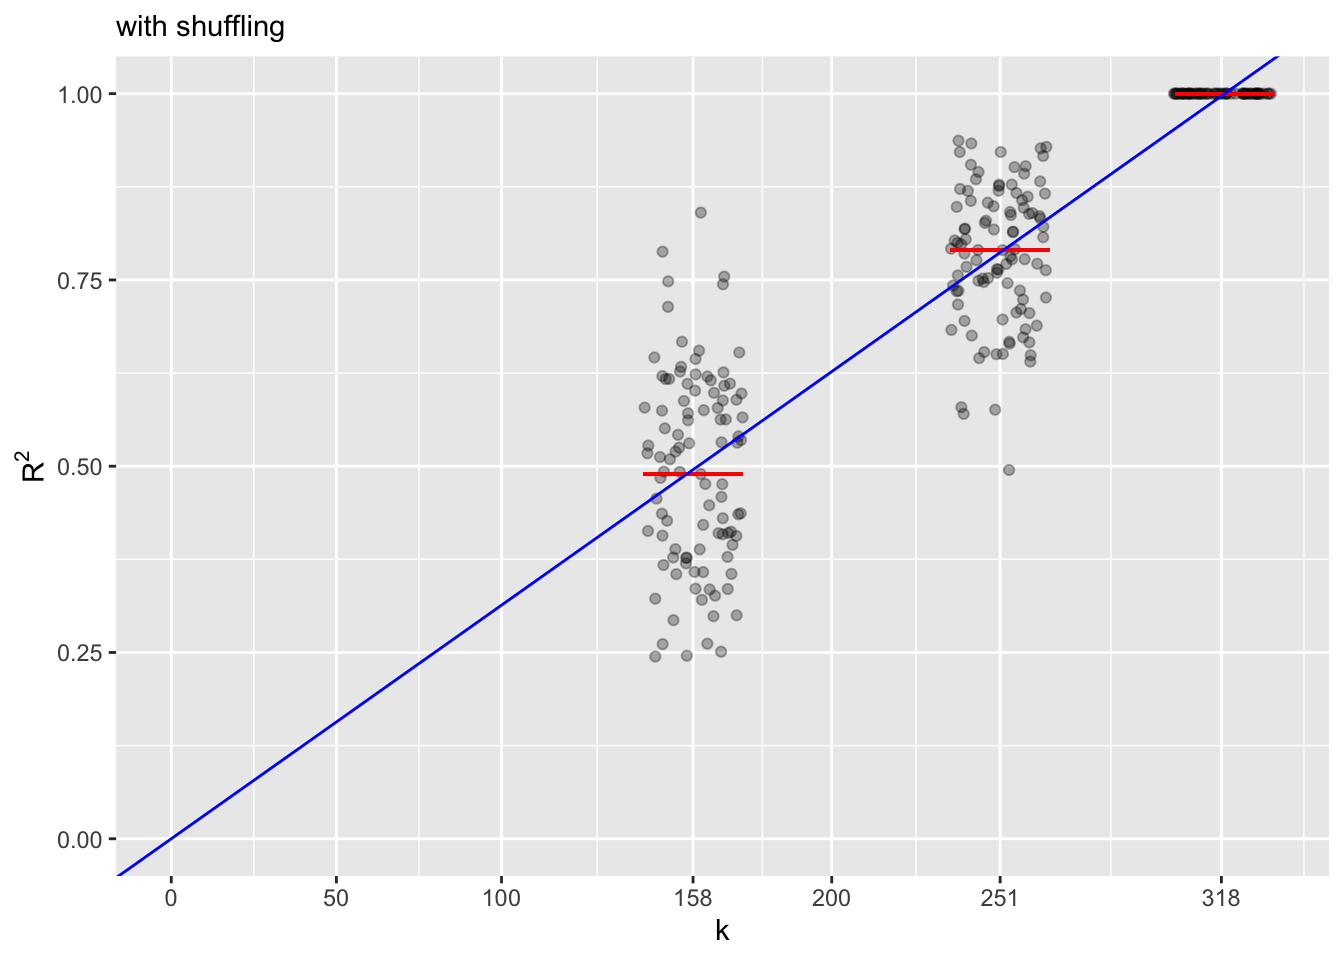
\includegraphics{./Reading-notes-lesson-29_files/figure-pdf/fig-amazon-book-shuffle-1.pdf}

}

\caption{\label{fig-amazon-book-shuffle}R\textsuperscript{2} from many
trials of three models,
\texttt{list\_price\ \textasciitilde{}\ shuffle(publisher)} and
\texttt{\textasciitilde{}\ shuffle(author)} and
\texttt{\textasciitilde{}shuffle(isbn\_10)}.}

\end{figure}

The blue diagonal line in Figure~\ref{fig-amazon-book-shuffle} shows the
theoretical average R\textsuperscript{2} as a function of the number of
model coefficients when the explanatory variable is randomized.
R\textsuperscript{2} will always be 1.0 when \(k=n\), that is, when the
number of coefficients is the same as the sample size.

Figure~\ref{fig-amazon-book-shuffle} suggests a way to distinguish
between R\textsuperscript{2} resulting from the ISBN-effect and
R\textsuperscript{2} that shows some true explanatory power: Check if
R\textsuperscript{2} is substantially above the blue diagonal line, that
is, check if R\textsuperscript{2}\(\gg \frac{k}{n-1}\) where \(k\) is
the number of model coefficients.

\hypertarget{the-f-statistic}{%
\section{The F statistic}\label{the-f-statistic}}

\(k\) and \(n\) provide the necessary context for proper interpretation
of R\textsuperscript{2}; all three numbers are needed to establish
whether R\textsuperscript{2} \(\gg \frac{k}{n-1}\) to rule out the ISBN
effect. The calculation is not difficult; the modeler always knows the
size \(n\) of the training data and can find \(k\) as the number of
coefficients in the model (not counting the Intercept term).

Perhaps a little easier than interpreting R\textsuperscript{2} is the
interpretation of another statistic, named F, which folds in the \(k\),
\(n\), and R\textsuperscript{2} into a single number:
\[F \equiv \frac{n-k-1}{k} \frac{\text{R}^2}{1 - \text{R}^2}\]
Figure~\ref{fig-amazon-book-shuffle-F} is a remake of
Figure~\ref{fig-amazon-book-shuffle} but using F instead of
R\textsuperscript{2}. The blue line, which had the formula
R\textsuperscript{2}\(= k/(n-1)\) in
Figure~\ref{fig-amazon-book-shuffle}, gets translated to the constant
value 1.0 in Figure~\ref{fig-amazon-book-shuffle-F}, regardless of
\(k\). To decide when a model points to a connection stronger than the
ISBN effect, the threshold F \(> 3\) is a good rule of thumb.
(Lesson~\ref{sec-lesson-37} introduces a more precise calculation for
the F threshold, which is built into statistical software and presented
as a ``\textbf{p-value}.'')

\begin{figure}

\sidecaption{\label{fig-amazon-book-shuffle-F}Like
Figure~\ref{fig-amazon-book-shuffle}, but using the F statistic to
summarize each trial.}

{\centering 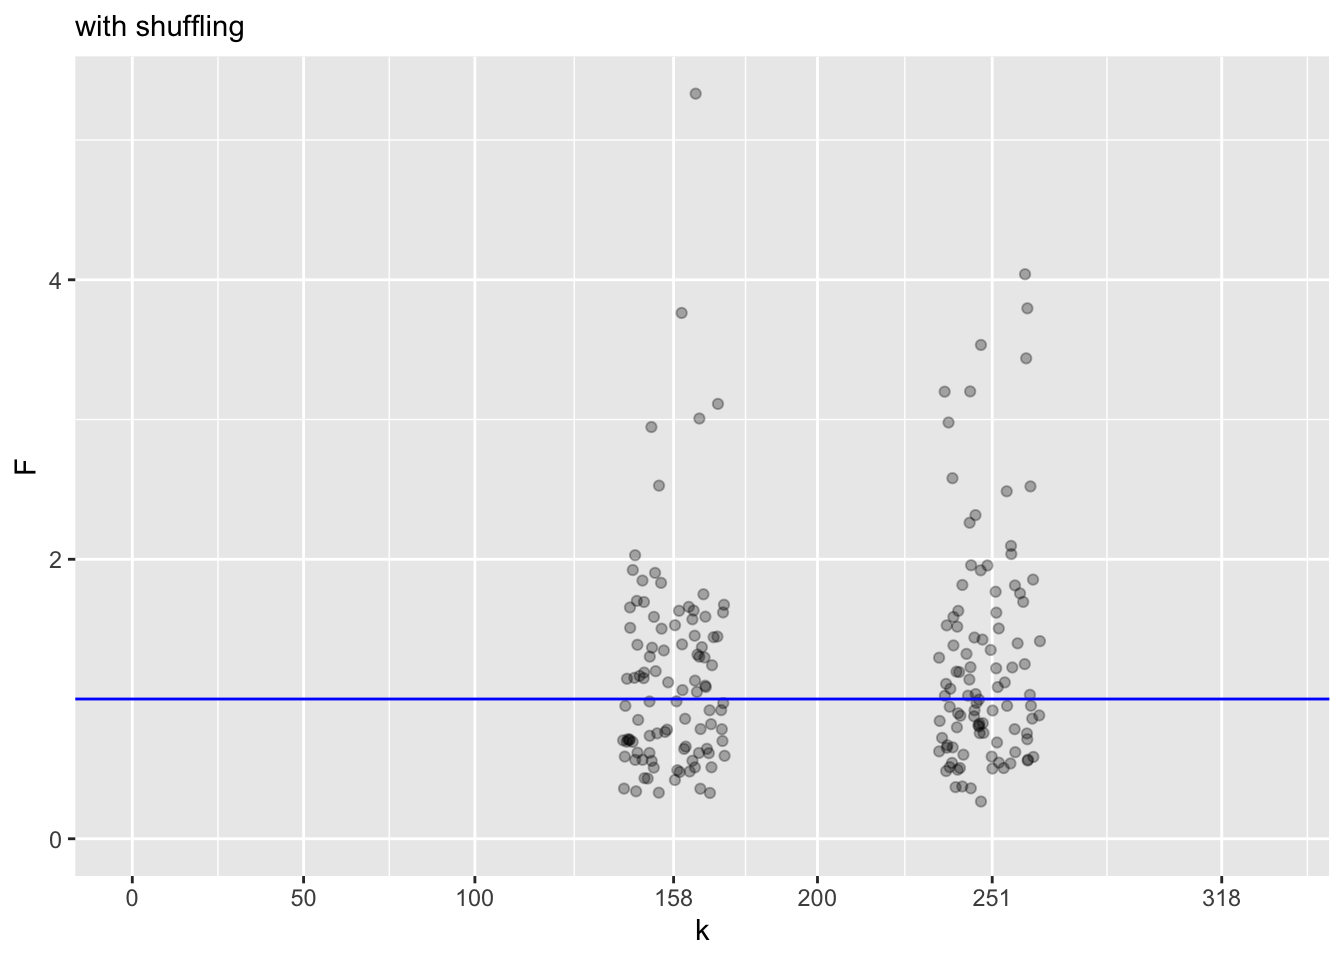
\includegraphics{./Reading-notes-lesson-29_files/figure-pdf/fig-amazon-book-shuffle-F-1.pdf}

}

\end{figure}

\begin{tcolorbox}[enhanced jigsaw, colbacktitle=quarto-callout-note-color!10!white, breakable, opacitybacktitle=0.6, colback=white, left=2mm, arc=.35mm, colframe=quarto-callout-note-color-frame, coltitle=black, toprule=.15mm, opacityback=0, leftrule=.75mm, bottomtitle=1mm, toptitle=1mm, titlerule=0mm, title=\textcolor{quarto-callout-note-color}{\faInfo}\hspace{0.5em}{Adjusted R\textsuperscript{2}}, rightrule=.15mm, bottomrule=.15mm]

Some fields, notably economics, prefer an alternative to F called
``\textbf{adjusted R\textsuperscript{2}}'' (or \(R^2_\text{adj}\)). The
adjustment comes from moving the raw R\textsuperscript{2} downward and
leftward, more-or-less in the direction of the blue line in
Figure~\ref{fig-amazon-book-shuffle}. This movement adjusts a raw
\(R^2\) that lies on the blue line to \(R^2_\text{adj} = 0\).

We leave the debate on the relative merits of using F or
\(R^2_\text{adj}\) their respective boosters. However, before getting
wrapped up in such debates, it is worth pointing out that
\(R^2_\text{adj}\) is just a rescaling of F.

\[R^2_\text{adj} = 1 - \frac{n-1}{k} \frac{R^2}{F}\ .\]

\end{tcolorbox}

\hypertarget{sec-partial-R2}{%
\section{Comparing models}\label{sec-partial-R2}}

Modelers are often in the position of having a model that they like but
are contemplating adding one or more additional explanatory variables.
To illustrate, consider the following models:

\begin{figure*}

\begin{itemize}
\tightlist
\item
  Model 1: \texttt{list\_price\ \textasciitilde{}\ 1}
\item
  Model 2: \texttt{list\_price\ \textasciitilde{}\ 1\ +\ hard\_paper}
\item
  Model 3:
  \texttt{list\_price\ \textasciitilde{}\ 1\ +\ hard\_paper\ +\ num\_pages}
\item
  Model 4:
  \texttt{list\_price\ \textasciitilde{}\ 1\ +\ hard\_paper\ +\ num\_pages\ +\ weight\_oz}
\end{itemize}

\end{figure*}

\begin{marginfigure}

{\centering 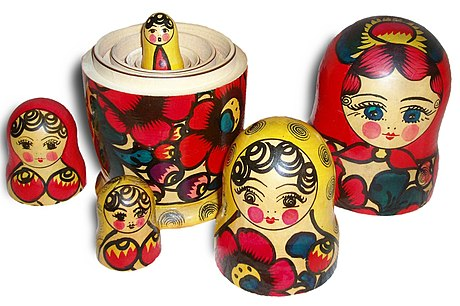
\includegraphics[width=1.53in,height=\textheight]{./www/Russian-Matroshka_no_bg.jpeg}

}

\caption{\label{fig-russian-dolls}Nesting Russian dolls}

\end{marginfigure}

All the explanatory variables in the smaller models also apply to the
bigger models. Such sets are said to be ``\textbf{nested}'' in much the
same way as for Russian dolls.

For a nested set of models, R\textsuperscript{2} can never decrease when
moving from a smaller model to a larger one---almost always, there is an
increase in R\textsuperscript{2}. To demonstrate:

\begin{figure*}

\begin{Shaded}
\begin{Highlighting}[]
\NormalTok{amazon\_books }\OtherTok{\textless{}{-}}\NormalTok{ amazon\_books }\SpecialCharTok{\%\textgreater{}\%} 
  \FunctionTok{select}\NormalTok{(list\_price, weight\_oz, num\_pages, hard\_paper) }\SpecialCharTok{\%\textgreater{}\%}
  \FunctionTok{filter}\NormalTok{(}\FunctionTok{complete.cases}\NormalTok{(.))}
\NormalTok{model1 }\OtherTok{\textless{}{-}} \FunctionTok{lm}\NormalTok{(list\_price }\SpecialCharTok{\textasciitilde{}} \DecValTok{1}\NormalTok{, }\AttributeTok{data=}\NormalTok{amazon\_books)}
\NormalTok{model2 }\OtherTok{\textless{}{-}} \FunctionTok{lm}\NormalTok{(list\_price }\SpecialCharTok{\textasciitilde{}} \DecValTok{1} \SpecialCharTok{+}\NormalTok{ weight\_oz, }\AttributeTok{data =}\NormalTok{ amazon\_books)}
\NormalTok{model3 }\OtherTok{\textless{}{-}} \FunctionTok{lm}\NormalTok{(list\_price }\SpecialCharTok{\textasciitilde{}} \DecValTok{1} \SpecialCharTok{+}\NormalTok{ weight\_oz }\SpecialCharTok{+}\NormalTok{ num\_pages, }\AttributeTok{data=}\NormalTok{amazon\_books)}
\NormalTok{model4 }\OtherTok{\textless{}{-}} \FunctionTok{lm}\NormalTok{(list\_price }\SpecialCharTok{\textasciitilde{}} \DecValTok{1} \SpecialCharTok{+}\NormalTok{ weight\_oz }\SpecialCharTok{+}\NormalTok{ num\_pages }\SpecialCharTok{+}\NormalTok{ hard\_paper, }\AttributeTok{data=}\NormalTok{amazon\_books)}
\end{Highlighting}
\end{Shaded}

\end{figure*}

\begin{Shaded}
\begin{Highlighting}[]
\FunctionTok{R2}\NormalTok{(model1)}
\end{Highlighting}
\end{Shaded}

\ttfamily 
\begin{tabular}{rrrrr}
\toprule
n & k & Rsquared & F & adjR2\\
\midrule
309 & 0 & 0 & NaN & 0\\
\bottomrule
\end{tabular} \normalfont
\bigskip

\begin{Shaded}
\begin{Highlighting}[]
\FunctionTok{R2}\NormalTok{(model2)}
\end{Highlighting}
\end{Shaded}

\ttfamily 
\begin{tabular}{rrrrr}
\toprule
n & k & Rsquared & F & adjR2\\
\midrule
309 & 1 & 0.16 & 57 & 0.15\\
\bottomrule
\end{tabular} \normalfont
\bigskip

\begin{Shaded}
\begin{Highlighting}[]
\FunctionTok{R2}\NormalTok{(model3)}
\end{Highlighting}
\end{Shaded}

\ttfamily 
\begin{tabular}{rrrrr}
\toprule
n & k & Rsquared & F & adjR2\\
\midrule
309 & 2 & 0.17 & 30 & 0.16\\
\bottomrule
\end{tabular} \normalfont
\bigskip

\begin{Shaded}
\begin{Highlighting}[]
\FunctionTok{R2}\NormalTok{(model4)}
\end{Highlighting}
\end{Shaded}

\ttfamily 
\begin{tabular}{rrrrr}
\toprule
n & k & Rsquared & F & adjR2\\
\midrule
309 & 3 & 0.17 & 21 & 0.16\\
\bottomrule
\end{tabular} \normalfont
\bigskip

When adding explanatory variables to a model, a good question is whether
the new variable(s) add to the ability to account for the variability in
the response variable. R\textsuperscript{2} never goes down when moving
from a smaller to a larger model, so we cannot rely on the increase in
R\textsuperscript{2}. A valuable technique called ``\textbf{Analysis of
Variance}'' (ANOVA for short) looks at the incremental change in
variance explained from a smaller model to a larger one. The increase
can be presented as an F statistic. To illustrate:

\begin{Shaded}
\begin{Highlighting}[]
\FunctionTok{anova\_summary}\NormalTok{(model1, model2, model3, model4)}
\end{Highlighting}
\end{Shaded}

\ttfamily 
\begin{tabular}{lrrrrrr}
\toprule
term & df.residual & rss & df & sumsq & statistic & p.value\\
\midrule
list\_price \textasciitilde{} 1 & 308 & 54531 & NA & NA & NA & NA\\
list\_price \textasciitilde{} 1 + weight\_oz & 307 & 46032 & 1 & 8499 & 57.2 & 0.00\\
list\_price \textasciitilde{} 1 + weight\_oz + num\_pages & 306 & 45466 & 1 & 566 & 3.8 & 0.05\\
list\_price \textasciitilde{} 1 + weight\_oz + num\_pages + hard\_paper & 305 & 45277 & 1 & 189 & 1.3 & 0.26\\
\bottomrule
\end{tabular} \normalfont
\bigskip

Focus on the column named \texttt{statistic}. This records the F
statistic. The move from Model 1 to Model 2 produces F=57, well above
the threshold described above and clearly indicating that the
\texttt{weight\_oz} variable accounts for some of the list price. Moving
from Model 2 to Model 3 creates a much less impressive F of 3.8. It is
as if the added explanatory variable, \texttt{num\_pages}, is just
barely pulling its own ``weight.'' Finally, moving from Model 3 to Model
4 produces a below-threshold F of 1.3. In other words, in the context of
\texttt{weight\_oz} and \texttt{num\_pages,} the \texttt{hard\_paper}
variable does not carry additional information about the list price.

The last column of the report, labeled \texttt{Pr(\textgreater{}F)},
translates F into a universal 0 to 1 scale called a p-value. A large F
produces a small p-value. The rule of thumb for reading p-values is that
a value \(p < 0.05\) indicates that the added variable brings new
information about the response variable. We will return to p-values and
the controversy they have entailed in Lessons 36 through 38.

\hypertarget{sec-lesson-30}{%
\chapter{Confounding}\label{sec-lesson-30}}

Many people are concerned that the chemicals used by lawn-greening
companies are a source of cancer or other illness. Imagine designing a
study that could confirm or refute this concern. The study would sample
households, some with a history of using lawn-greening chemicals and
others that have never used them. The question for the study designers:
What variables to record?

An obvious answer: record both chemical use and a measure of health
outcome, say whether anyone in that household has developed cancer in
the last five years. We will suppose that the two possible levels of
grass treatment are ``organic'' or ``chemicals.'' As for illness, the
levels will be ``cancer'' or ``not.''

Here are two very simple DAGs describing possible theories:

\[\text{illness} \leftarrow \text{grass treatment}\ \ \ \ \text{ or   }\ \ \ \ \ \text{illness} \rightarrow \text{grass treatment}\]

The DAG on the left expresses the belief among people who think chemical
grass treatment might cause cancer. But belief is not necessarily
reality, so we should consider the right-hand DAG. For example, one way
to avoid the possibility of
\(\text{illness} \rightarrow \text{grass treatment}\) is to include only
households where cancer (if any) started \emph{after} the grass
treatment. Note that we are not ignoring the right-hand DAG; we are
using the study design to disqualify it.

The statistical thinker knows that covariates are important. But which
covariates? Answering that requires knowing a lot about the ``domain,''
that is, how things connect in the world. Such knowledge helps in
thinking about the bigger picture and, in particular, possible
covariates that connect plausibly to the response variable and the
primary explanatory variable, grass treatment.

For now, suppose that the study designers have not yet become
statistical thinkers and have rushed out to gather data on illness and
grass treatment. Here are a few rows from the data (which we have
simulated for this example):

\ttfamily 
\begin{tabular}{ll}
\toprule
grass & illness\\
\midrule
organic & not\\
chemicals & not\\
chemicals & not\\
chemicals & not\\
organic & not\\
\addlinespace
organic & not\\
organic & not\\
organic & not\\
chemicals & cancer\\
organic & not\\
\bottomrule
\end{tabular} \normalfont
\bigskip

Analyzing such data is straightforward. First, check the overall cancer
rate:

\begin{Shaded}
\begin{Highlighting}[]
\CommentTok{\# overall cancer rate}
\FunctionTok{lm}\NormalTok{(}\FunctionTok{zero\_one}\NormalTok{(illness, }\AttributeTok{one=}\StringTok{"cancer"}\NormalTok{) }\SpecialCharTok{\textasciitilde{}} \DecValTok{1}\NormalTok{, }\AttributeTok{data =}\NormalTok{ Cancer\_data) }\SpecialCharTok{\%\textgreater{}\%} \FunctionTok{coef}\NormalTok{()}
\end{Highlighting}
\end{Shaded}

\begin{verbatim}
(Intercept) 
      0.026 
\end{verbatim}

In these data, 2.6\% of the sampled households had cancer in the last
five years. How does the grass treatment affect that rate?

\begin{Shaded}
\begin{Highlighting}[]
\NormalTok{mod }\OtherTok{\textless{}{-}} \FunctionTok{lm}\NormalTok{(}\FunctionTok{zero\_one}\NormalTok{(illness, }\AttributeTok{one=}\StringTok{"cancer"}\NormalTok{) }\SpecialCharTok{\textasciitilde{}}\NormalTok{ grass, }\AttributeTok{data =}\NormalTok{ Cancer\_data)}
\FunctionTok{coefficients}\NormalTok{(mod)}
\end{Highlighting}
\end{Shaded}

\begin{verbatim}
 (Intercept) grassorganic 
  0.01246883   0.02258960 
\end{verbatim}

For households whose lawn treatment is ``organic,'' the risk of cancer
is higher by 2.3 percentage points compared to households that treat
their grass with chemicals. We were expecting the reverse, but it is
what the data show. On the other hand, there is sampling variability to
take into account. Look at the confidence intervals:

\begin{Shaded}
\begin{Highlighting}[]
\FunctionTok{conf\_interval}\NormalTok{(mod)}
\end{Highlighting}
\end{Shaded}

\ttfamily 
\begin{tabular}{lrr}
\toprule
term & .lwr & .upr\\
\midrule
(Intercept) & -0.0031034 & 0.028041\\
grassorganic & 0.0024692 & 0.042710\\
\bottomrule
\end{tabular} \normalfont
\bigskip

The confidence interval on \texttt{grassorganic} does not include zero,
but it comes close. So might the chemical treatment of grass be
protective against cancer? Only at this point do the study designers do
what they should have from the start: think about covariates.

One theory---just a theory---is this: Green grass is not a necessity, so
the households who treat their lawn with chemicals tend to have money to
spare. Wealthier people also tend to have better health, partly because
of better access to health care. Another factor is that wealthier people
can live in less polluted neighborhoods and are less likely to work in
dangerous conditions, such as exposure to toxic chemicals. Such a link
between wealth and illness points to a DAG hypothesis where
``\texttt{wealth}'' influences how the household's \texttt{grass} is
treated and \texttt{wealth} similarly influences the risk of developing
\texttt{cancer}. Like this:

\includegraphics{./Reading-notes-lesson-30_files/figure-pdf/unnamed-chunk-6-1.pdf}

A description of this structure of causality is, ``The effect of grass
treatment on illness is \textbf{confounded} by wealth.'' The
\href{https://languages.oup.com/google-dictionary-en/}{Oxford Languages}
dictionary offers two definitions of ``confound.''

\begin{enumerate}
\def\labelenumi{\arabic{enumi}.}
\tightlist
\item
  \emph{Cause surprise or confusion in someone, especially by acting
  against their expectations.}
\item
  \emph{Mix up something with something else so that the individual
  elements become difficult to distinguish.}
\end{enumerate}

This second definition carries the statistical meaning of ``confound.''

The first definition seems relevant to our story since the protagonist
expected that chemical use would be associated with higher cancer rates
and was surprised to find otherwise. But, the statistical thinker does
not throw up her hands when dealing with mixed-up causal factors.
Instead, she uses modeling techniques to untangle the influences of
various factors.

Using covariates in models is one such technique. Our wised-up study
designers go back to collect a covariate representing household wealth.
Here is a glimpse at the updated data.

\ttfamily 
\begin{tabular}{rll}
\toprule
wealth & grass & illness\\
\midrule
1.4283990 & organic & not\\
0.0628559 & chemicals & not\\
0.4382804 & chemicals & not\\
0.6084487 & chemicals & not\\
0.8033695 & organic & not\\
\addlinespace
-0.9367287 & organic & not\\
0.6664468 & organic & not\\
-1.2445977 & organic & not\\
-1.3194594 & chemicals & cancer\\
-1.6162391 & organic & not\\
\bottomrule
\end{tabular} \normalfont
\bigskip

Having measured \texttt{wealth}, we can use it as a covariate in the
model of \texttt{illness}:

\begin{Shaded}
\begin{Highlighting}[]
\FunctionTok{lm}\NormalTok{(}\FunctionTok{zero\_one}\NormalTok{(illness, }\AttributeTok{one=}\StringTok{"cancer"}\NormalTok{) }\SpecialCharTok{\textasciitilde{}}\NormalTok{ grass }\SpecialCharTok{+}\NormalTok{ wealth, }\AttributeTok{data =}\NormalTok{ Cancer\_data) }\SpecialCharTok{\%\textgreater{}\%}
  \FunctionTok{conf\_interval}\NormalTok{()}
\end{Highlighting}
\end{Shaded}

\ttfamily 
\begin{tabular}{lrr}
\toprule
term & .lwr & .upr\\
\midrule
(Intercept) & 0.0246811 & 0.0574819\\
grassorganic & -0.0450811 & -0.0009699\\
wealth & -0.0568093 & -0.0356454\\
\bottomrule
\end{tabular} \normalfont
\bigskip

With \texttt{wealth} as a covariate, the model shows that (all other
things being equal) ``organic'' lawn treatment reduces cancer risk.
However, we do not see this directly from the \texttt{grass} and
\texttt{illness} variables because all other things are not equal:
wealthier people are more likely to use chemical lawn treatment. (Keep
in mind that this is \textbf{simulated data}. Do not conclude from this
example anything about the safety of the chemicals used for lawn
greening.)

\begin{tcolorbox}[enhanced jigsaw, colbacktitle=quarto-callout-note-color!10!white, breakable, opacitybacktitle=0.6, colback=white, left=2mm, arc=.35mm, colframe=quarto-callout-note-color-frame, coltitle=black, toprule=.15mm, opacityback=0, leftrule=.75mm, bottomtitle=1mm, toptitle=1mm, titlerule=0mm, title=\textcolor{quarto-callout-note-color}{\faInfo}\hspace{0.5em}{Example: The flu vaccine}, rightrule=.15mm, bottomrule=.15mm]

As you know, people are encouraged to get vaccinated before flu season.
This recommendation is particularly emphasized for older adults, say, 60
and over.

In 2012, the \emph{Lancet}, a leading medical journal, published a
\href{https://www.thelancet.com/journals/laninf/article/PIIS1473-3099(11)70295-X/fulltext}{systematic
examination and comparison of many previous studies}.
{\marginnote{\begin{footnotesize}Such a study of earlier studies is
called a \emph{meta-analysis}.\end{footnotesize}}} The \emph{Lancet}
article describes a hypothesis that existing flu vaccines may not be as
effective as was originally found.

\begin{quote}
\emph{A series of observational studies undertaken between 1980 and 2001
attempted to estimate the effect of seasonal influenza vaccine on rates
of hospital admission and mortality in {[}adults 65 and older{]}.
Reduction in all-cause mortality after vaccination in these studies
ranged from 27\% to 75\%. In 2005, these results were questioned after
reports that increasing vaccination in people aged 65 years or older did
not result in a significant decline in mortality. Five different
research groups in three countries have shown that these early
observational studies had substantially overestimated the mortality
benefits in this age group because of unrecognized confounding. This
error has been attributed to a healthy vaccine recipient effect:
reasonably healthy older adults are more likely to be vaccinated, and a
small group of frail, undervaccinated elderly people contribute
disproportionately to deaths, including during periods when influenza
activity is low or absent.}
\end{quote}

\begin{figure}[H]

{\centering 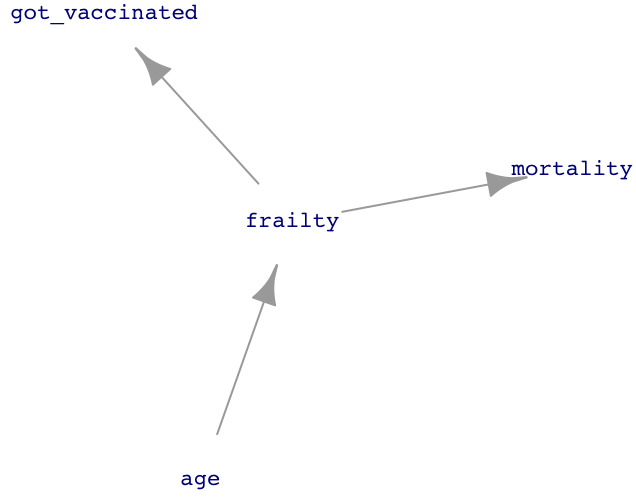
\includegraphics[width=2.12in,height=\textheight]{./www/healthy-vaccine-dag.png}

}

\caption{\label{fig-healthy-vaccine}A DAG diagramming the ``healthy
vaccine recipient'' effect}

\end{figure}

Figure~\ref{fig-healthy-vaccine} presents a network of causal influences
that could shape the ``healthy vaccine recipient.'' People are more
likely to become frail as they get older. Frail people are \emph{less}
likely to get vaccinated, but more likely to die in the next few months.
The result is that vaccination is associated with reduced mortality,
even if there is no direct link between vaccination and mortality.

\end{tcolorbox}

\hypertarget{block-that-path}{%
\section{Block that path!}\label{block-that-path}}

Let us look more generally at the possible causal connections among
three variables, which we will call X, Y, and C. We will stipulate that
X points causally toward Y and that C is a possible covariate. Like all
DAGs, there cannot be a cycle of causation. These conditions leave three
distinct DAGs that do not have a cycle, shown in
Figure~\ref{fig-three-dags-cancer}.

\begin{figure*}

\begin{minipage}[t]{0.33\linewidth}

{\centering 

\raisebox{-\height}{

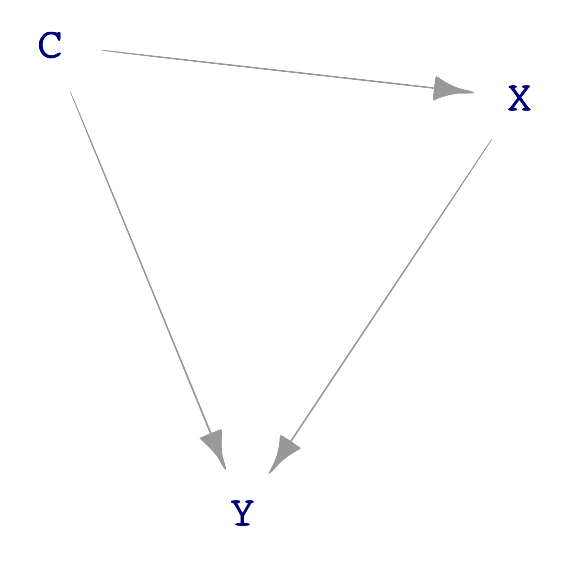
\includegraphics[width=1.92in,height=\textheight]{./www/abc-dag-1.png}

}

}

\subcaption{\label{fig-three-dags-cancer-1}C is a confounder.}
\end{minipage}%
%
\begin{minipage}[t]{0.33\linewidth}

{\centering 

\raisebox{-\height}{

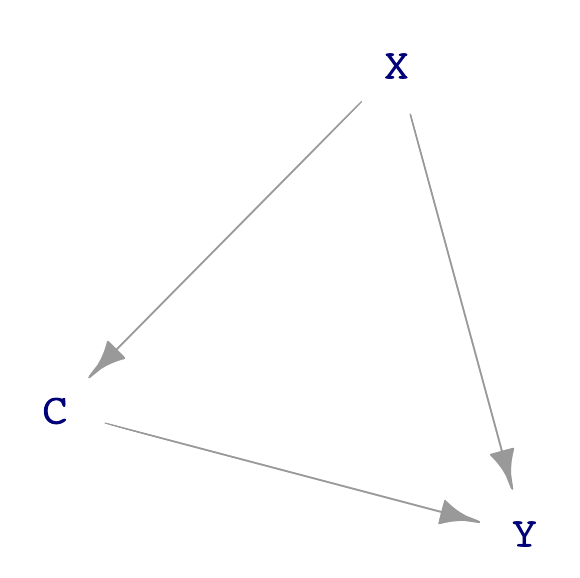
\includegraphics[width=1.93in,height=\textheight]{./www/abc-dag-2.png}

}

}

\subcaption{\label{fig-three-dags-cancer-2}C is a mechanism.}
\end{minipage}%
%
\begin{minipage}[t]{0.33\linewidth}

{\centering 

\raisebox{-\height}{

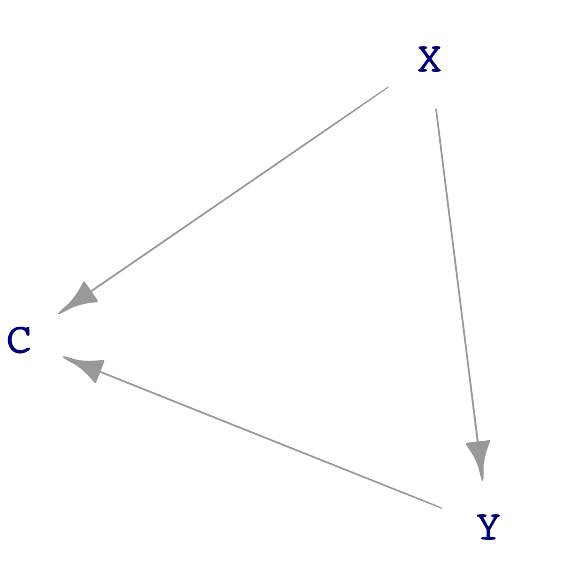
\includegraphics[width=1.92in,height=\textheight]{./www/abc-dag-3.png}

}

}

\subcaption{\label{fig-three-dags-cancer-3}C is a consequence.}
\end{minipage}%

\caption{\label{fig-three-dags-cancer}Three different DAGs connecting X,
Y, and C.}

\end{figure*}

C plays a different role in each of the three dags. In sub-figure (a), C
causes both X and Y. In (b), part of the way that X influences Y is
\emph{through} C. We say, in this case, ``C is a mechanism by which X
causes Y. In sub-figure (c), C does not cause either X or Y. Instead, C
is a consequence of both X and Y.\footnote{In any given real-world
  context, good practice calls for considering each possible DAG
  structure and concocting a story behind it. Such stories will
  sometimes be implausible, but there can also be surprises that give
  the modeler new insight.}

To understand how a DAG informs whether or not to include a covariate,
It will help to give general names to some of the sub-structures seen in
the Figure~\ref{fig-three-dags-cancer} DAGs. \textbf{?@fig-dag-paths}
shows some of these sub-structures, removing other links that are not
part of the structure.

\begin{figure*}

\begin{minipage}[t]{0.25\linewidth}

{\centering 

\raisebox{-\height}{

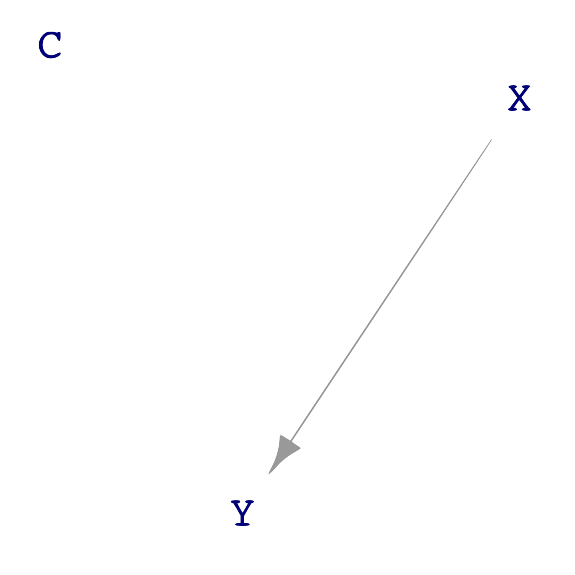
\includegraphics[width=1.92in,height=\textheight]{./www/abc-direct.png}

}

}

\subcaption{\label{fig-dags-paths-1}Direct causal link from X to Y}
\end{minipage}%
%
\begin{minipage}[t]{0.25\linewidth}

{\centering 

\raisebox{-\height}{

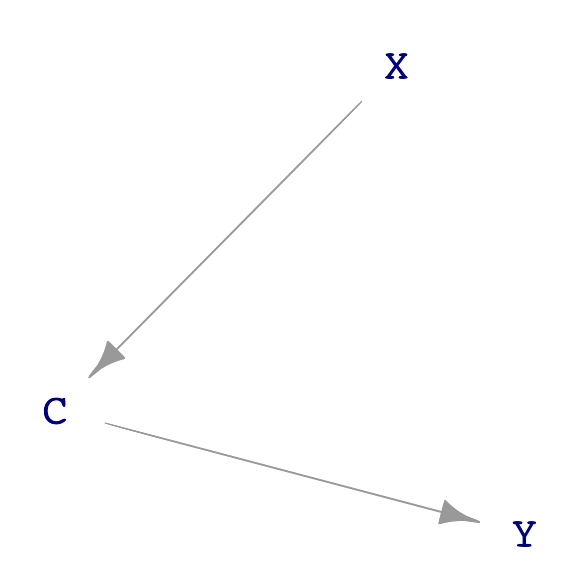
\includegraphics[width=1.93in,height=\textheight]{./www/abc-causal.png}

}

}

\subcaption{\label{fig-dags-paths-2}Causal path from X through C to Y}
\end{minipage}%
%
\begin{minipage}[t]{0.25\linewidth}

{\centering 

\raisebox{-\height}{

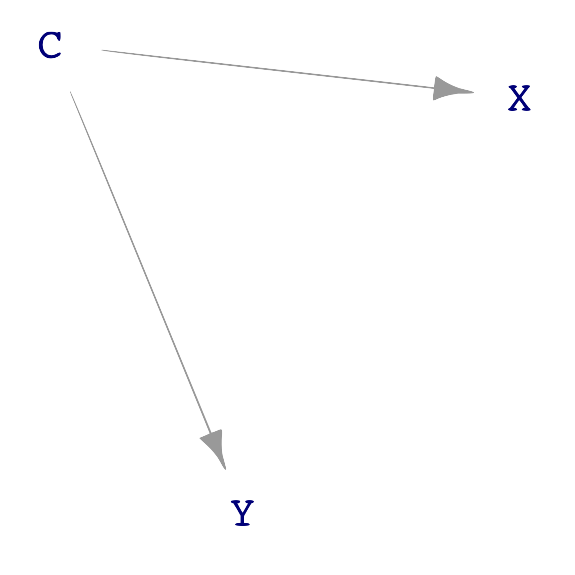
\includegraphics[width=1.92in,height=\textheight]{./www/abc-correlating.png}

}

}

\subcaption{\label{fig-dags-paths-3}Correlating path connecting X and Y
via C}
\end{minipage}%
%
\begin{minipage}[t]{0.25\linewidth}

{\centering 

\raisebox{-\height}{

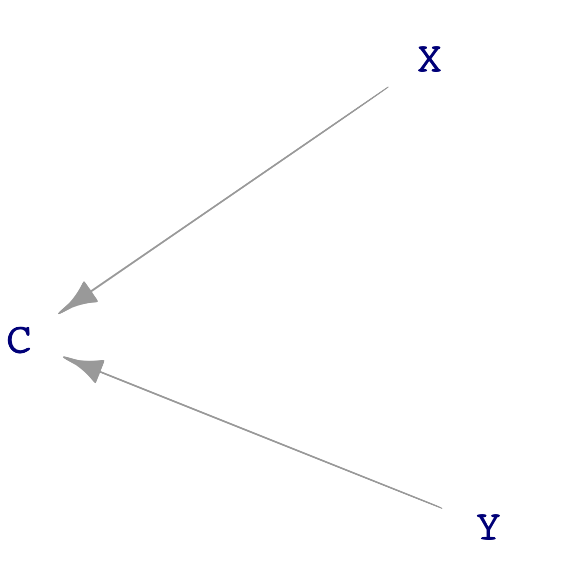
\includegraphics[width=1.92in,height=\textheight]{./www/abc-collider.png}

}

}

\subcaption{\label{fig-dags-paths-4}C as a consequence of X and Y}
\end{minipage}%

\caption{\label{fig-dags-paths}Sub-structures seen in
Figure~\ref{fig-three-dags-cancer}.}

\end{figure*}

\begin{itemize}
\item
  A ``\textbf{direct causal link}'' between X and Y. There are no
  intermediate nodes.
\item
  A ``\textbf{causal path}'' from C to X and on to Y. A causal path is
  one where, starting at the originating node, flow along the arrows can
  get to the terminal node, passing through all intermediate nodes.
\item
  A ``\textbf{correlating path}'' from Y through X to C. Correlating
  paths are distinct from causal paths because, in a correlating path,
  there is no way to get from one end to the other by following the
  flows.
\item
  A ``\textbf{collider}'' \texttt{wealth}. In other words, both X and Y
  are causes of C.
\end{itemize}

Look back to Figure~\ref{fig-three-dags-cancer}(a), where
\texttt{wealth} is a confounder. A confounder is always an intermediate
node in a \emph{correlating path}.

Including a covariate either blocks or opens the pathway on which that
covariate lies. Which it will be depends on the kind of pathway. A
causal path, as in Figure~\ref{fig-dags-paths}(b), is blocked by
including the covariate. Otherwise, it is open. A correlating path
(\textbf{?@fig-dags-path}(c)) is similar: the path is open unless the
covariate is included in the model. A colliding path, as in
Figure~\ref{fig-dags-paths}(d), is blocked \emph{unless} the covariate
is included---the opposite of a causal path.

Often, covariates are selected to block all paths except the direct link
between the explanatory and response variable. This means \emph{do}
include the covariate if it is on a correlating path and \emph{do not}
include it if the covariate is at the collision point.

As for a causal path, the choice depends on what is to be studied.
Consider the DAG drawn in Figure~\ref{fig-three-dags-cancer}(b),
reproduced here for convenience:

\begin{marginfigure}

{\centering 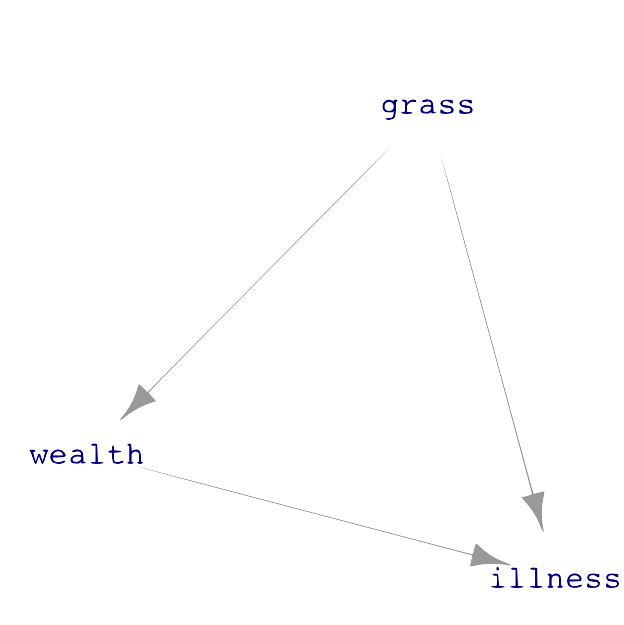
\includegraphics[width=2.08in,height=\textheight]{./www/grass-dag-2.png}

}

\end{marginfigure}

\texttt{grass} influences \texttt{illness} through two distinct paths:

\begin{enumerate}
\def\labelenumi{\roman{enumi}.}
\tightlist
\item
  the direct link from \texttt{grass} to \texttt{illness}.
\item
  the causal pathway from \texttt{grass} through \texttt{wealth} to
  \texttt{illness}.
\end{enumerate}

Admittedly, it is far-fetched that choosing to green the grass makes a
household wealthier, but focus on the topology of the DAG and not the
unlikeliness of this specific causal scenario.

There is no way to block a direct link from an explanatory variable to a
response. If there were a reason to do this, the modeler probably
selected the wrong explanatory variable.

But there is a genuine choice to be made about whether to block pathway
(ii). If the interest is the purely biochemical link between
grass-greening chemicals and illness, then block pathway (ii). However,
if the interest is in the \emph{total} effect of \texttt{grass} and
\texttt{illness}, including both biochemistry and the sociological
reasons why \texttt{wealth} influences \texttt{illness}, then leave the
pathway open.

\begin{tcolorbox}[enhanced jigsaw, colbacktitle=quarto-callout-warning-color!10!white, breakable, opacitybacktitle=0.6, colback=white, left=2mm, arc=.35mm, colframe=quarto-callout-warning-color-frame, coltitle=black, toprule=.15mm, opacityback=0, leftrule=.75mm, bottomtitle=1mm, toptitle=1mm, titlerule=0mm, title=\textcolor{quarto-callout-warning-color}{\faExclamationTriangle}\hspace{0.5em}{In draft: Some resources}, rightrule=.15mm, bottomrule=.15mm]

https://towardsdatascience.com/causal-effects-via-dags-801df31da794

https://towardsdatascience.com/causal-effects-via-the-do-operator-5415aefc834a

\end{tcolorbox}

\hypertarget{sec-lesson-31}{%
\chapter{Spurious correlation}\label{sec-lesson-31}}

\href{https://books.google.com/ngrams}{Google NGram} provides a quick
way to track word usage in books over the decades.
Figure~\ref{fig-ngram} shows the NGram for three statistical words:
coefficient, correlation, and regression.

\begin{figure}

\sidecaption{\label{fig-ngram}Google NGram for ``coefficient,''
``correlation,'' and ``regression.''}

{\centering 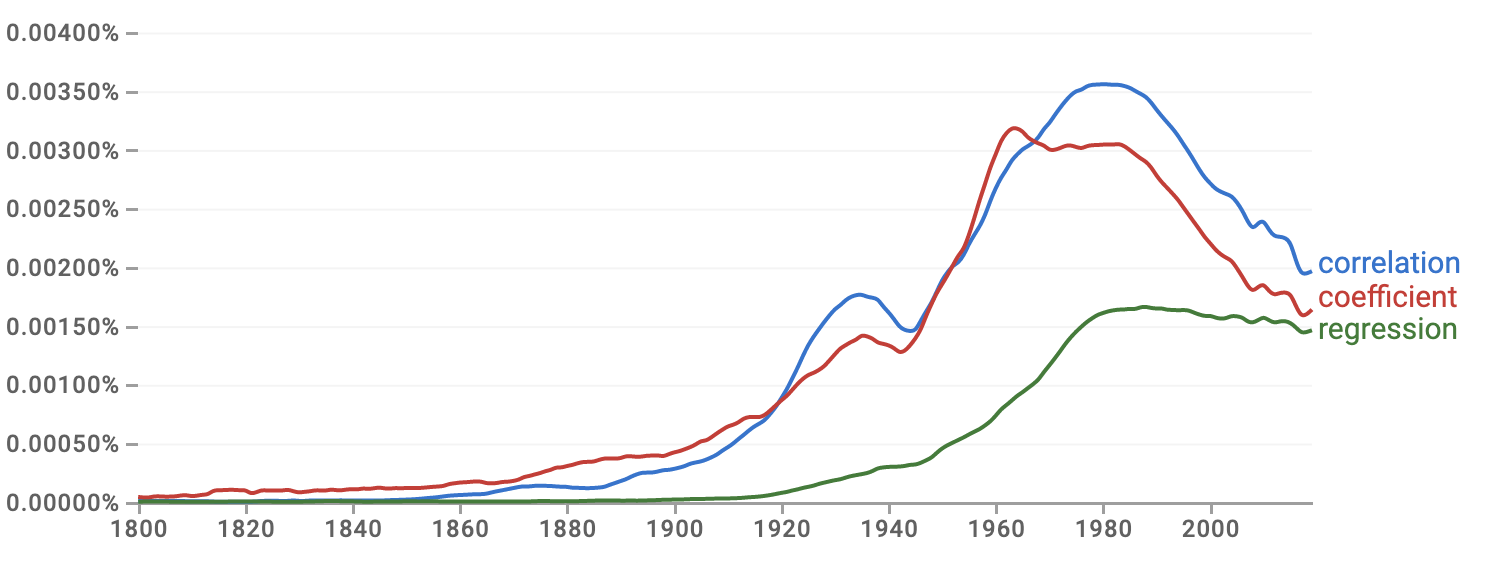
\includegraphics[width=4.98in,height=\textheight]{./www/correlation-ngram.png}

}

\end{figure}

The use of ``correlation'' started in the mid to late 1800s, reached an
early peak in the 1930s, then peaked again around 1980. ``Correlation''
is tracked closely by ``coefficient.'' This parallel track might seem
evident to historians of statistics; the quantitative measure called the
``\textbf{correlation coefficient}'' was introduced by Francis Galton in
1888 and quickly became a staple of statistics textbooks.

In contrast to mainstream statistics textbooks, ``correlation'' barely
appears in these lessons (until this chapter). There is a good reason
for this. Although the correlation coefficient measures the ``strength''
of the relationship between two variables, it is a special case of a
more general and powerful method that appears throughout these Lessons:
regression modeling.

Figure~\ref{fig-ngram} shows that ``regression'' got a later start than
correlation. That is likely because it took 30-40 years before it was
appreciated that correlation could be generalized. Furthermore,
regression is more mathematically complicated than correlation, so
practical use of regression relied on computing, and computers started
to become available only around 1950.

\hypertarget{correlation}{%
\section{Correlation}\label{correlation}}

A dictionary is a starting point for understanding the use of a word.
Here are four definitions of ``correlation'' from general-purpose
dictionaries.

\begin{quote}
``\emph{A relation existing between phenomena or things or between
mathematical or statistical variables which tend to vary, be associated,
or occur together in a way not expected on the basis of chance alone}''
Source:
\href{https://www.merriam-webster.com/dictionary/correlation}{Merriam-Webster
Dictionary}
\end{quote}

\begin{quote}
``\emph{A connection between two things in which one thing changes as
the other does}'' Source:
\href{https://www.oxfordlearnersdictionaries.com/us/definition/english/correlation}{Oxford
Learner's Dictionary}
\end{quote}

\begin{quote}
``\emph{A connection or relationship between two or more things that is
not caused by chance. A positive correlation means that two things are
likely to exist together; a negative correlation means that they are
not.}'' Source:
\href{https://www.macmillandictionary.com/us/dictionary/american/correlation}{Macmillan
dictionary}
\end{quote}

\begin{quote}
``A mutual relationship or connection between two or more things,''
``interdependence of variable quantities.'' Source: {[}Oxford
Languages{]}
\end{quote}

All four definitions use ``connection'' or ``relation/relationship.''
That is at the core of ``correlation.'' Indeed, ``relation'' is part of
the word ``correlation.'' One of the definitions uses ``causes''
explicitly, and the everyday meaning of ``connection'' and ``relation''
tend to point in this direction. The phrase ``one thing changes as the
other does'' is close to the idea of causality, as is
``interdependence.:

Three of the definitions use the words ``vary,'' ``variable,'' or
``changes.'' The emphasis on variation also appears directly in a close
statistical synonym for correlation: ``covariance.''

Two of the definitions refer to ``chance,'' that correlation ``is not
caused by chance,'' or ``not expected on the basis of chance alone.''
These phrases suggest to a general reader that correlation, since not
based on chance, must be a matter of fate: pre-determination and the
action of causal mechanisms.

We can put the above definitions in the context of four major themes of
these Lessons:

\begin{itemize}
\tightlist
\item
  Quantitative description of relationships
\item
  Variation
\item
  Sampling variation
\item
  Causality
\end{itemize}

Correlation is about relationships; the ``correlation coefficient'' is a
way to describe a straight-line relationship quantitatively. The
correlation coefficient addresses the tandem variation of quantities,
or, more simply stated, how ``one thing changes as the other does.''

To a statistical thinker, the concern about ``chance'' in the
definitions is not about fate but reliability. Sampling variation can
lead to the appearance of a pattern in some samples of a process that is
not seen in other samples of that same process. Reliability means that
the pattern will appear in a large majority of samples.

\begin{tcolorbox}[enhanced jigsaw, colbacktitle=quarto-callout-note-color!10!white, breakable, opacitybacktitle=0.6, colback=white, left=2mm, arc=.35mm, colframe=quarto-callout-note-color-frame, coltitle=black, toprule=.15mm, opacityback=0, leftrule=.75mm, bottomtitle=1mm, toptitle=1mm, titlerule=0mm, title=\textcolor{quarto-callout-note-color}{\faInfo}\hspace{0.5em}{Note}, rightrule=.15mm, bottomrule=.15mm]

One of the better explanations of ``correlation'' appears in an 1890
article by Francis Galton, who invented the correlation coefficient.
Since the explanation is more than a century old, some words will be
unfamiliar to the modern reader. For example, a ``clerk'' is an office
worker. An ``omnibus'' is merely a means of public transportation today.

\begin{quote}
\emph{Two clerks leave their office together and travel homewards in the
same and somewhat unpunctual omnibus every day. They both get out of the
omnibus at the same halting-place, and thence both walk by their several
ways to their respective homes. \ldots{} The upshot is that when either
clerk arrives at his home later than his average time, there is some
reason to expect that the other clerk will be late also, because the
retardation of the first clerk may have been wholly or partly due to
slowness of the omnibus on that day, which would equally have retarded
the second clerk. Hence their unpunctualities are related. If the
omnibus took them both very near to their homes, the relation would be
very close. If they lodged in the same house and the omnibus dropped
them at its door, the relation would become identity.}
\end{quote}

\begin{quote}
\emph{The problems of \ldots{} correlation deal wholly with departures
or variations ; they pay no direct regard to the central form from which
the departures or variations are measured. If we were measuring
statures, and had made a mark on our rule at a height equal to the
average height of the race of persons whom we were considering, then it
would be the distance of the top of each man's head from that mark,
upward or downward as the case might be, that is wanted for our use, and
not its distance upward from the ground.}\footnote{Francis Galton (1890)
  ``Kinship and Correlation'' \emph{The North American Review} 150(401)
  \href{https://www.jstor.org/stable/25101964}{URL}}
\end{quote}

\end{tcolorbox}

\hypertarget{spurious-causation}{%
\section{Spurious causation}\label{spurious-causation}}

\begin{marginfigure}

{\centering 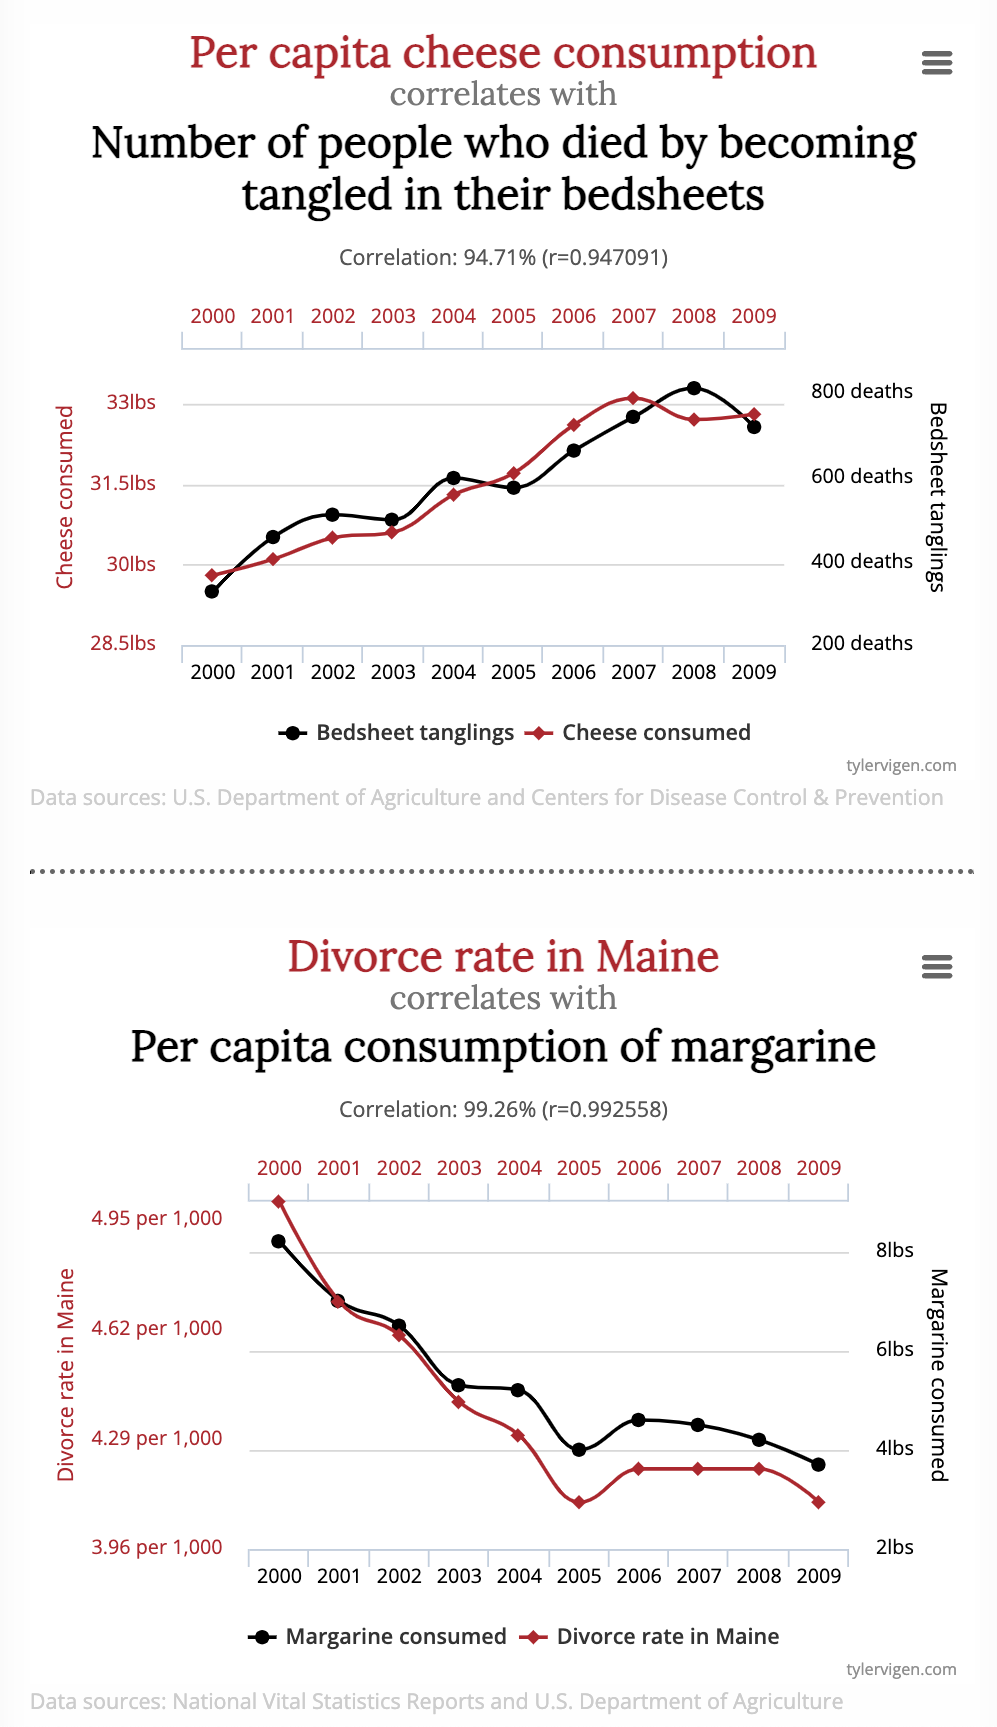
\includegraphics[width=3.32in,height=\textheight]{./www/spurious-correlations.png}

}

\caption{\label{fig-spurious-correlation}Two examples from the
\href{http://www.tylervigen.com/spurious-correlations}{Spurious
correlations} website}

\end{marginfigure}

The ``Spurious correlations'' website
\url{http://www.tylervigen.com/spurious-correlations} provides
entertaining examples of correlations gone wrong. The running gag is
that the two correlated variables have no reasonable association, yet
the correlation coefficient is very close to its theoretical maximum of
1.0. Typically, one of the variables is morbid, as in
Figure~\ref{fig-spurious-correlation}.

\begin{marginfigure}

{\centering 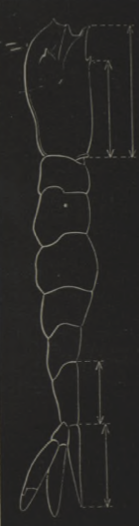
\includegraphics[width=1.5\textwidth,height=\textheight]{./www/shrimp-organs.png}

}

\caption{\label{fig-telson-tergum}The telson and tergum are anatomical
parts of the shrimp. Their locations are marked at the bottom. Source:
Weldon 1888}

\end{marginfigure}

According to Aldrich (1995)\^{}{[}John Aldrich (1994) ``Correlations
Genuine and Spurious in Pearson and Yule'' \emph{Statistical Science}
10(4) \href{https://www.jstor.org/stable/2246135}{URL} the idea of
\textbf{spurious correlations} appears first in an 1897 paper by
statistical pioneer and philosopher of science Karl Pearson. The
correlation coefficient method was published only in 1888, and,
understandably, early users encountered pitfalls. One very early user,
W.F.R. Weldon, published a study in 1892 on the correlations between the
sizes of organs, such as the tergum and telson in shrimp. (See
Figure~\ref{fig-telson-tergum}.)

\begin{figure}

{\centering 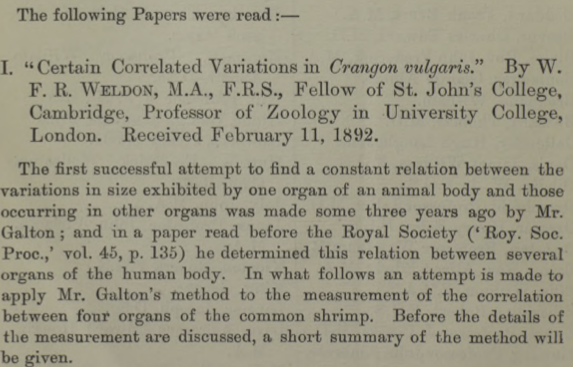
\includegraphics[width=0.8\textwidth,height=\textheight]{./www/shrimp-correlations.png}

}

\end{figure}

Pearson noticed a distinctive feature of Weldon's method. Weldon
measured the tergum and telson as a fraction of the overall body length.

Figure~\ref{fig-shrimp-dag} shows one possible DAG interpretation where
\texttt{telson} and \texttt{tergum} are \emph{not} connected by any
causal path. Similarly, \texttt{length} is exogenous with no causal path
between it and either \texttt{telson} or \texttt{tergum}.

\begin{Shaded}
\begin{Highlighting}[]
\NormalTok{shrimp\_dag }\OtherTok{\textless{}{-}} \FunctionTok{dag\_make}\NormalTok{(}
\NormalTok{  tergum }\SpecialCharTok{\textasciitilde{}} \FunctionTok{unif}\NormalTok{(}\AttributeTok{min=}\DecValTok{2}\NormalTok{, }\AttributeTok{max=}\DecValTok{3}\NormalTok{),}
\NormalTok{  telson }\SpecialCharTok{\textasciitilde{}} \FunctionTok{unif}\NormalTok{(}\AttributeTok{min=}\DecValTok{4}\NormalTok{, }\AttributeTok{max=}\DecValTok{5}\NormalTok{),}
\NormalTok{  length }\SpecialCharTok{\textasciitilde{}} \FunctionTok{unif}\NormalTok{(}\AttributeTok{min=}\DecValTok{40}\NormalTok{, }\AttributeTok{max=}\DecValTok{80}\NormalTok{), }
\NormalTok{  x }\SpecialCharTok{\textasciitilde{}}\NormalTok{ tergum}\SpecialCharTok{/}\NormalTok{length }\SpecialCharTok{+} \FunctionTok{exo}\NormalTok{(.}\DecValTok{01}\NormalTok{),}
\NormalTok{  y }\SpecialCharTok{\textasciitilde{}}\NormalTok{ telson}\SpecialCharTok{/}\NormalTok{length }\SpecialCharTok{+} \FunctionTok{exo}\NormalTok{(.}\DecValTok{01}\NormalTok{)}
\NormalTok{)}
\CommentTok{\# dag\_draw(shrimp\_dag, seed=101, vertex.label.cex=1)}
\NormalTok{knitr}\SpecialCharTok{::}\FunctionTok{include\_graphics}\NormalTok{(}\StringTok{"www/telson{-}tergum.png"}\NormalTok{)}
\end{Highlighting}
\end{Shaded}

\begin{marginfigure}

{\centering 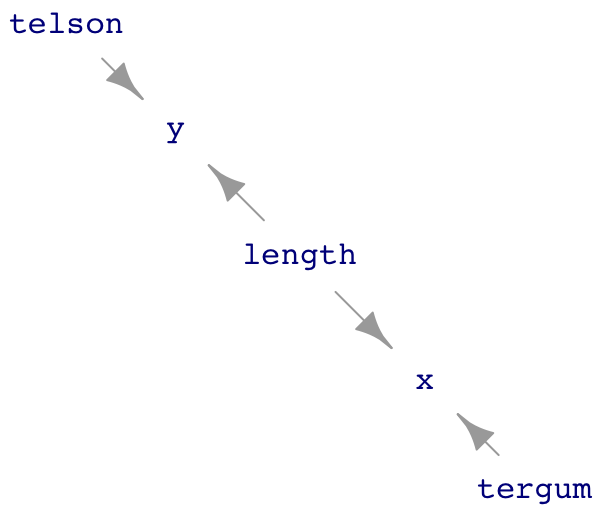
\includegraphics[width=2.01in,height=\textheight]{./www/telson-tergum.png}

}

\caption{\label{fig-shrimp-dag}DAG for the shrimp measurements.}

\end{marginfigure}

The Figure~\ref{fig-shrimp-dag} shows a hypothesis where there is no
causal relationship between telson and tergum. Pearson wondered whether
dividing those quantities by \texttt{length} to produce variables
\texttt{x} and \texttt{y}, might induce a correlation. Weldon had found
a correlation coefficient between \texttt{x} and \texttt{y} of about
0.6. Pearson estimated that dividing by \texttt{length} would induce a
correlation between \texttt{x} and \texttt{y} of about 0.4-0.5, even if
telson and tergum are not causally connected.

We can confirm Pearson's estimate by sampling from the DAG and modeling
\texttt{y} by \texttt{x}. The confidence interval on \texttt{x} shows a
relationship between \texttt{x} and \texttt{y}. In 1892, before the
invention of regression, the correlation coefficient would have been
used. In retrospect, we know the correlation coefficient is a simple
scaling of the \texttt{x} coefficient.

\begin{Shaded}
\begin{Highlighting}[]
\NormalTok{Sample }\OtherTok{\textless{}{-}} \FunctionTok{sample}\NormalTok{(shrimp\_dag, }\AttributeTok{size=}\DecValTok{1000}\NormalTok{)}
\FunctionTok{lm}\NormalTok{(y }\SpecialCharTok{\textasciitilde{}}\NormalTok{ x, }\AttributeTok{data=}\NormalTok{Sample) }\SpecialCharTok{\%\textgreater{}\%} \FunctionTok{conf\_interval}\NormalTok{()}
\end{Highlighting}
\end{Shaded}

\ttfamily 
\begin{tabular}{lrr}
\toprule
term & .lwr & .upr\\
\midrule
(Intercept) & 0.0457665 & 0.0522715\\
x & 0.6147549 & 0.7566114\\
\bottomrule
\end{tabular} \normalfont
\bigskip

\begin{Shaded}
\begin{Highlighting}[]
\FunctionTok{cor}\NormalTok{(y }\SpecialCharTok{\textasciitilde{}}\NormalTok{ x, }\AttributeTok{data=}\NormalTok{Sample)}
\end{Highlighting}
\end{Shaded}

\begin{verbatim}
[1] 0.514812
\end{verbatim}

Pearson's 1897 work precedes the earliest conception of DAGs by three
decades. An entire century would pass before DAGs came into widespread
use. However, from the DAG of Figure~\ref{fig-shrimp-dag}{]} in front of
us, we can see that \texttt{length} is a common cause of \texttt{x} and
\texttt{y}.

Within 20 years of Pearson's publication, a mathematical technique
called ``\textbf{partial correlation}'' was in use that could deal with
this particular problem of spurious correlation. The key is that the
model should include \texttt{length} as a covariate. The covariate
correctly blocks the path from \texttt{x} to \texttt{y} via
\texttt{length}.

\begin{Shaded}
\begin{Highlighting}[]
\FunctionTok{lm}\NormalTok{(y }\SpecialCharTok{\textasciitilde{}}\NormalTok{ x }\SpecialCharTok{+}\NormalTok{ length, }\AttributeTok{data=}\NormalTok{Sample) }\SpecialCharTok{\%\textgreater{}\%} \FunctionTok{conf\_interval}\NormalTok{()}
\end{Highlighting}
\end{Shaded}

\ttfamily 
\begin{tabular}{lrr}
\toprule
term & .lwr & .upr\\
\midrule
(Intercept) & 0.1507687 & 0.1635108\\
x & -0.0362598 & 0.0833543\\
length & -0.0013975 & -0.0012508\\
\bottomrule
\end{tabular} \normalfont
\bigskip

The confidence interval on the \texttt{x} coefficient includes zero once
\texttt{length} is included in the model. So the data, properly
analyzed, show no correlation between telson and tergum.

In this case, ``spurious correlation'' stems from using an inappropriate
method. This situation, identified 130 years ago and addressed a century
ago, is still a problem for those who use the correlation coefficient.
Although regression allows the incorporation of covariates, the
correlation coefficient does not.

\begin{tcolorbox}[enhanced jigsaw, colbacktitle=quarto-callout-note-color!10!white, breakable, opacitybacktitle=0.6, colback=white, left=2mm, arc=.35mm, colframe=quarto-callout-note-color-frame, coltitle=black, toprule=.15mm, opacityback=0, leftrule=.75mm, bottomtitle=1mm, toptitle=1mm, titlerule=0mm, title=\textcolor{quarto-callout-note-color}{\faInfo}\hspace{0.5em}{Time series analysis}, rightrule=.15mm, bottomrule=.15mm]

Some spurious correlations, such as those presented on the
\href{http://www.tylervigen.com/spurious-correlations}{eponymous
website}, can also be attributed to methodological error.

One source of error was identified in 1904 by F.E. Cave-Browne-Cave in
her paper ``On the influence of the time factor on the correlation
between the barometric heights at stations more than 1000 miles apart,''
published in the Proceedings of the Royal Society. ``Miss Cave,'' as she
was referred to in 1917 and 1921, respectively by eminent statisticians
William Sealy Gosset (who published under the name ``Student'') and
George Udny Yule, also offered a solution to the problem. Her solution
is very much in the tradition of ``\textbf{time-series analysis},'' a
contemporary specialized area of statistics.

The unlikeliness of the correlations on the website is another clue to
their origin as methodological. Nobody woke up one morning with the
hypothesis that cheese consumption and bedsheet mortality are related.
Instead, the correlation is the product of a search among many
miscellaneous records. Imagine that data were available on 10,000
annually tabulated variables for the last decade. These 10,000 variables
create the opportunity for 50 million pairs of variables. Even if none
of these 50 million pairs have a genuine relationship, sampling
variation will lead to some of them having a strong correlation
coefficient.

In statistics, such a blind search is called the ``multiple comparisons
problem.'' Ways to address the problem have been available since the
1950s. (We will return to this topic under the label ``false discovery''
in Lesson~\ref{sec-lesson-38}.) Multiple comparisons can be used as a
trick, as with the website. However, multiple comparisons also arise
naturally in some fields. For example, in molecular genetics,
``micro-arrays'' make a hundred thousand simultaneous measurements of
gene expression. Correlations in the expression of two genes give a clue
to cellular function and disease. With so many pairs available, multiple
comparisons will be an issue.

\end{tcolorbox}

\hypertarget{correlation-implies-causation.}{%
\section{``Correlation implies
causation.''}\label{correlation-implies-causation.}}

Francis Galton's 1890 example of the clerks on the bus introduces
``correlation'' as a causality story. The bus trip causes variation in
commute times. Two clerks riding the same bus will have correlated
commute times. In the dictionary definitions of ``correlation'' at the
start of the Lesson, the words ``connection,'' ``relationship,'' and
``interdependence'' suggests causal connections.

\begin{marginfigure}

{\centering 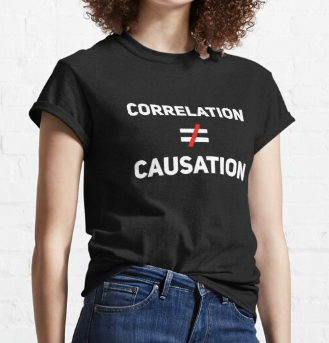
\includegraphics[width=1.1in,height=\textheight]{./www/correlation-tee-shirt.png}

}

\end{marginfigure}

Insofar as the dictionary definitions of correlation suggest a causal
relationship, they are at odds with the statistical mainstream, which
famously holds that ``correlation does not imply causation.'' This view
is so entrenched that it appears on tee shirts, one style of which is
available for sale by the American Statistical Association.

The statement ``A is not B'' can be valid only if we know what A and B
are. We have a handle on the meaning of ``correlation.'' So what is the
meaning of ``causation?''

Dictionaries define ``causation'' using the word ``cause.'' So we look
there for guidance.

\begin{quote}
A person or thing that gives rise to an action, phenomenon, or
condition. Source: Oxford Languages
\end{quote}

\begin{quote}
An event, thing, or person that makes something happen. Source:
Macmillan Dictionary
\end{quote}

\begin{quote}
A person or thing that acts, happens, or exists in such a way that some
specific thing happens as a result; the producer of an effect. Source:
Dictionary.com
\end{quote}

Interpreting these definitions requires making sense of ``give rise
to,'' ``makes happen,'' or ``happens as a result.'' All of them are
synonyms for ``cause.''

This circularity produces a muddle. Centuries of philosophical debate
have yet to clarify things much.

Still, we can do something. The point of view of these Lessons is to
support decision-making. Causation is a valuable concept for
decision-making, particularly in cases where the decision-maker is
considering an \emph{intervention}. With this as an anchor, a pragmatic
definition of ``causation'' is available:

\begin{quote}
Causation describes a class of hypotheses that DAGs can represent. In
that representation, a causal relationship between two nodes X and Y is
marked by a causal path connecting X to Y. In
Lesson~\ref{sec-lesson-30}, we defined ``causal path'' in terms of the
directions of arrows in a DAG.\footnote{We will consider a ``direct
  causal link'' to be a form of causal path.} A definitive demonstration
of a causal relationship between X and Y is that intervening to change X
results reliably in a change in Y, \emph{all other nodes not on the
causal path being held constant.} (Lesson~\ref{sec-lesson-32} treats the
methodology behind this definitive sign.)
\end{quote}

Whether or not a definitive demonstration is feasible is not directly
relevant to the decision-maker. A decision-maker acts under the guidance
of one or more hypotheses. A good rule of thumb for decision-makers is
to be guided only by plausible hypotheses. Whether a hypothesis is
plausible is a matter of informed belief. A definitive demonstration
should sharpen that belief. If no such definitive demonstration is
available, the decision-maker must rely on alternative sources for
belief. Austin Bradford Hill (1898-1991), an epidemiologist and eminent
statistician, famously published a
\href{https://en.wikipedia.org/wiki/Bradford_Hill_criteria}{list of nine
criteria} that support belief in a causal hypothesis.

Using my definition of causation, and in marked disagreement with many
statisticians, I submit that

\begin{quote}
\emph{Correlation implies causation.}
\end{quote}

``Correlation implies causation'' is not the same as saying, ``A
correlation between A and B implies that A causes B.'' That statement is
false. For instance, it might be instead that B causes A. Alternatively,
there might be a common cause C for both A and B. Or, C might be a
collider between A and B.

There is no mechanism to produce correlation that I am aware of, other
than the sources of spurious correlation described previously, that does
not involve causation in some way.

::: \{.callout-note\} \#\# So why do many statisticians say different?

Historically, the rise of the expression ``correlation does not imply
causation''---Figure~\ref{fig-ngram-corr-is-not-cause} shows the ngram
since the 1888 invention of the correlation coefficient---comes
\emph{after} the peak in the use of the word ``correlation.''

\begin{figure}

\sidecaption{\label{fig-ngram-corr-is-not-cause}Google NGram showing the
rise in the use of the phrases ``correlation does not imply causation,''
and ``correlation is not causation'' in recent decades.}

{\centering 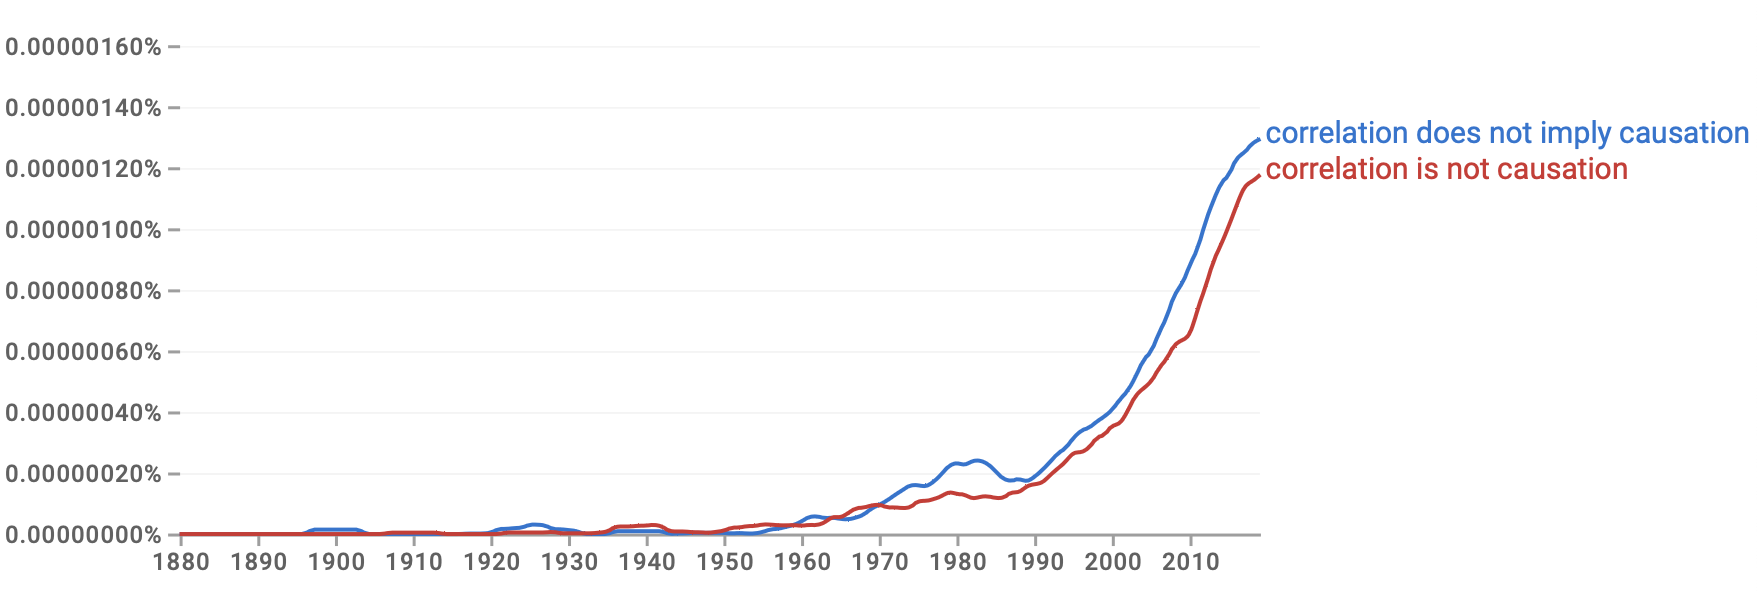
\includegraphics[width=5.86in,height=\textheight]{./www/ngram-correlation-not-causation.png}

}

\end{figure}

The first documented use of the phrase is from 1900. It comes in a
review of the second edition of a book, \emph{The Grammar of Science},
by Karl Pearson (whom we have met before in this Lesson).

\emph{The Grammar of Science} is a metaphysically oriented prescription
for a new type of science. It posited that sciences such as physics or
chemistry unnecessarily drew on metaphors for causation, such as
``force.'' Instead, the book advocated another framework as more
appropriate, eschewing causation in favor of descriptions of
``perceptions'' with probability.

Pearson illustrates his antipathy toward causation with an example of an
ash tree in his garden:

\begin{quote}
{[}T{]}he causes of its growth might be widened out into a description
of the various past stages of the universe. One of the causes of its
growth is the existence of my garden, which is conditioned by the
existence of the metropolis {[}London{]}; another cause is the nature of
the soil, gravel approaching the edge of the clay, which again is
conditioned by the geological structure and past history of the earth.
The causes of any \emph{individual} thing thus widen out into the
unmanageable history of the universe. \emph{The Grammar of Science},
2/e, p.~131
\end{quote}

It should not be surprising that the field of statistics, which uses
probability very extensively as a description, and that developed
correlation as a measure of probability, would advocate for more general
use of its approach. In this spirit, I read ``correlation does not imply
causation'' as ``our new science framework of probability and
correlation replaces the antiquated framework of causation.'' Outside of
statistics, however, probability is merely a tool; causation does indeed
have practical use. All the more so for decision-makers.

\hypertarget{sec-lesson-32}{%
\chapter{Experiment and random assignment}\label{sec-lesson-32}}

In its everyday meaning, the word ``experiment'' is similar in meaning
to the word ``experience.'' As a verb, to experiment means to ``try out
new concepts or ways of doing things.'' As a noun, an experiment is a
``course of action tentatively adopted without being sure of the
outcome: the farm is an ongoing experiment in sustainable living.'' Both
quotes are from the
\href{https://languages.oup.com/google-dictionary-en/}{Oxford
Languages}, which provides examples of each: ``the designers
experimented with new ideas in lighting'' or ``the farm is an ongoing
experiment in sustainable living.''

From movies and other experiences, people associate experiments with
science. Indeed, one of the dictionary definitions of ``experiment'' is:
``a scientific procedure undertaken to make a discovery, test a
hypothesis, or demonstrate a known fact.''

Almost all the knowledge needed to perform a scientific experiment
relates to the science itself: what reagents to use, how to measure the
concentration of a neurotransmitter, how to administer a drug safely,
and so on. This is why people who carry out scientific procedures are
trained primarily in their area of science.

\begin{tcolorbox}[enhanced jigsaw, colbacktitle=quarto-callout-note-color!10!white, breakable, opacitybacktitle=0.6, colback=white, left=2mm, arc=.35mm, colframe=quarto-callout-note-color-frame, coltitle=black, toprule=.15mm, opacityback=0, leftrule=.75mm, bottomtitle=1mm, toptitle=1mm, titlerule=0mm, title=\textcolor{quarto-callout-note-color}{\faInfo}\hspace{0.5em}{Example: Malaria and bed nets}, rightrule=.15mm, bottomrule=.15mm]

In many parts of the world, malaria is a major cause of disability and
death. Economists who study ways to relieve poverty have a simple,
plausible theory: reducing the effect of illnesses such as malaria will
have an impact on poverty rates, since healthier people are more
productive and reduced uncertainty can help them amass capital to invest
to increase production further.

There are many possible ways to reduce the burden of malaria.
Vaccination (although effective vaccines have been hard to develop),
insect control using pesticides (which can cause environmental
problems), etc. One simple intervention is the use of bed nets; screen
nets deployed at night by draping over the bed and its occupant. Still,
there are reasons why distributing bed nets may not be effective; people
might use them incorrectly or for other purposes such as fishing. People
might not be able to afford them, but giving them away might signal that
they have no value.

To find out, try it: do an experiment. For instance, run a trial program
where nets are given away to everyone in an area and observed whether
and to what extent rates of malarial illness go down.

Such a trial is certainly an experiment. But it may not be the best way
to get meaningful information.

\end{tcolorbox}

\hypertarget{replication}{%
\section{Replication}\label{replication}}

To understand some of the contribution that statistical thinking can
make to experiment, recall our earlier definition:

\begin{quote}
\emph{Statistic thinking is the explanation/description of variation} in
the context of \emph{what remains unexplained/undescribed.}
\end{quote}

A key concept that statistical thinking brings to experiment is the idea
of \textbf{variation}. Simply put, a good experiment should involve some
variation. The simplest way to create variation is to repeat each
experimental trial multiple times. This is called
``\textbf{replication}.''

\hypertarget{example-replicated-bed-net-trials}{%
\section{Example: Replicated bed net
trials}\label{example-replicated-bed-net-trials}}

One way to improve the simple experiment bed net described above is to
carry out many trials. One reason is that the results from any single
trial might be shaped by accidental or particular circumstances: the
weather in the trial area was less favorable to mosquito reproduction;
another government agency decided to help out by spraying pesticides
broadly, and so on. Setting up trials in different areas can help to
balance out these influences.

Replicated trials also allow us to estimate the size of the variability
caused by the accidental or particular factors. To illustrate, suppose a
single trial is done and the rate of malarial illness goes down by 5
percentage points. What can we conclude? The result is promising but we
can't rule out that it is due to accidental factors other than bed nets.
Why not? Because we have no idea how much unexplained variation is in
play.

\marginnote{\begin{footnotesize}

\begin{margintable}

\end{margintable}

\textbf{?@tbl-bed-net} shows data from four imagined trials of the
effect of bed nets. (Reduction by a negative number, like -1, is an
\emph{increase}.) The mean reduction is 3 percentage points, but this
number is not much use unless we can put it in the context of sampling
variation. Conducting multiple trials gives us a handle on the amount of
sampling variation. By We can easilyNow we know something about the
amount of variation due to site-to-site factors. The replication
introduces \emph{observed} variation in results, the observed variation
can be quantified and used to place the overall trend in context.

Using the regression framework makes it easy to estimate the amount of
sampling variation. The mean reduction corresponds to the coefficient
from the model \texttt{reduction\ \textasciitilde{}\ 1}.

\begin{Shaded}
\begin{Highlighting}[]
\FunctionTok{lm}\NormalTok{(reduction }\SpecialCharTok{\textasciitilde{}} \DecValTok{1}\NormalTok{, }
     \AttributeTok{data=}\NormalTok{Bed\_net\_data) }\SpecialCharTok{\%\textgreater{}\%} 
  \FunctionTok{coef}\NormalTok{()}
\end{Highlighting}
\end{Shaded}

\begin{verbatim}
(Intercept) 
          3 
\end{verbatim}

\begin{Shaded}
\begin{Highlighting}[]
\FunctionTok{lm}\NormalTok{(reduction }\SpecialCharTok{\textasciitilde{}} \DecValTok{1}\NormalTok{, }
     \AttributeTok{data=}\NormalTok{Bed\_net\_data) }\SpecialCharTok{\%\textgreater{}\%} 
  \FunctionTok{conf\_interval}\NormalTok{()}
\end{Highlighting}
\end{Shaded}

\ttfamily 
\begin{tabular}{lrr}
\toprule
term & .lwr & .upr\\
\midrule
(Intercept) & 1 & 5\\
\bottomrule
\end{tabular} \normalfont
\bigskip

The observed 3 percentage point mean reduction in the incidence of
malaria does stand out from the noise: the confidence interval does not
include zero. In these (imagined) data, we have confidence that we have
seen a signal.

\hypertarget{control}{%
\section{Control}\label{control}}

However, there is still a problem with the design of the imagined
bed-net experiment. What if the year the experiment was done was
unusually dry, reducing the mosquito population and, with it, the rate
of malaria infection? Then we don't know whether the observed 3 point
reduction is due to the weather or the bed nets, or even something else,
e.g.~better nutrition due to a drop in international prices for rice.

We need to measure what the change in malarial infection would have been
without the bed-net intervention. Care needs to be taken here. If the
trial sites were rural, it would not be appropriate to look at malarial
rates in urban areas where there was no bed-net program. We want to
compare the trial sites with non-trial sites where the intervention was
not carried out, so-called ``\textbf{control}'' sites. The
\texttt{With\_controls} data frame imagines what data might look like if
in half the sites no bed-net program was involved.

\hypertarget{tbl-bed-net-controls}{}
\ttfamily 
\begin{table}
\caption{\label{tbl-bed-net-controls}With\_controls }\tabularnewline

\centering
\begin{tabular}{lrl}
\toprule
site & reduction & nets\\
\midrule
A & 2 & control\\
B & 8 & treatment\\
C & 4 & treatment\\
D & 1 & treatment\\
E & -1 & control\\
\addlinespace
F & -2 & control\\
G & 0 & control\\
H & 2 & treatment\\
I & 3 & treatment\\
J & 2 & control\\
\bottomrule
\end{tabular}
\end{table}
 \normalfont
\bigskip

The proper regression model for the \texttt{With\_controls} data is
\texttt{reduction\ \textasciitilde{}\ treatment}:

\begin{Shaded}
\begin{Highlighting}[]
\FunctionTok{lm}\NormalTok{(reduction }\SpecialCharTok{\textasciitilde{}}\NormalTok{ nets, }
       \AttributeTok{data=}\NormalTok{With\_controls) }\SpecialCharTok{\%\textgreater{}\%} 
  \FunctionTok{coef}\NormalTok{() }
\end{Highlighting}
\end{Shaded}

\begin{verbatim}
  (Intercept) netstreatment 
          0.2           3.4 
\end{verbatim}

\begin{Shaded}
\begin{Highlighting}[]
\FunctionTok{lm}\NormalTok{(reduction }\SpecialCharTok{\textasciitilde{}}\NormalTok{ nets, }
       \AttributeTok{data=}\NormalTok{With\_controls) }\SpecialCharTok{\%\textgreater{}\%} 
  \FunctionTok{conf\_interval}\NormalTok{() }
\end{Highlighting}
\end{Shaded}

\ttfamily 
\begin{tabular}{lrr}
\toprule
term & .lwr & .upr\\
\midrule
(Intercept) & -2.200 & 2.6\\
netstreatment & 0.058 & 6.7\\
\bottomrule
\end{tabular} \normalfont
\bigskip

The effect of the bed nets is summarized by the \texttt{netstreatment}
coefficient, which compares the \texttt{reduction} between the
\texttt{treatment} and \texttt{control} groups. In this new (imagined)
data frame, the confidence interval on \texttt{netstreatment} touches
very close to zero; the signal is just barely discernible from the
noise.

The reader might wonder why, in moving to the controlled design, the ten
sites were not all treated with nets and another ten or so sites found
to use as the control. Perhaps, even, the control sites could be
selected as villages nearby to the bed net villages.

One reason is pragmatic: the larger study would require more effort and
money. The larger study might be worthwhile; larger \(n\) would
presumably narrow the confidence interval. Another reason, to be
expanded on in the next section, is that the treatment and control sites
should be as similar as possible. This can be surprising hard to
achieve. Other factors such as the enthusiasm or skepticism of the town
leaders toward public-health interventions might be behind the choice of
the original sites for the bed-net program. The control sites might be
towns that turned down the original offer of the bed-net program and,
accordingly, have different attitudes toward public health.

\hypertarget{example-testing-the-salk-polio-vaccine}{%
\section{Example: Testing the Salk polio
vaccine}\label{example-testing-the-salk-polio-vaccine}}

Today, most children are vaccinated against polio, though a smaller
fraction than in previous years. This might be because symptomatic polio
is very rare, lessening the perceived urgency of protecting against it.
Partly, the reduction reflects the growth in the ``anti-vax'' movement,
which became especially notable with the advent of COVID-19.

The first US polio epidemic occurred in 1916, just two years before the
COVID-like ``Spanish flu'' pandemic.\footnote{``Spanish'' is in quotes
  because Spain was not the source of the pandemic.} Up through the
early 1950s, polio injured or killed hundreds of thousands of people,
particularly children. Anxiety about the disease was similar to that
seen in the first year of the COVID-19 pandemic.

There were many attempts to develop a vaccine against polio. Jonas Salk
created the first really promising vaccine, the promise being based on
laboratory tests. To establish the safety and effectiveness of the Salk
vaccine, it needed to be tried in the field, with people. Two
organizations, the US Public Health Service and the National Foundation
for Infantile Paralysis got together to organize a clinical field trial
which, all told, involved two-million students in grades 1 through 3.

The two studies involved both a treatment and a control group. In some
school districts, students in grades 1 and 3 were held as controls. The
treatment group was students in grade 2 whose parents gave consent. We
will call this ``Study 1.'' In other school districts, the study design
was different: the parents of all students in all three grades were
asked for consent. The students with parental consent were then randomly
split into two groups: a treatment and a control. Call this ``Study 2.''

The Study 2 design might seem inefficient; it reduced the number of
children receiving the vaccine because half of the children with
parental consent were left unvaccinated. On the other hand, it might be
that children from families who consent to be given a vaccine are
different in a systematic way from children whose families refuse, just
as today's anti-vax families might be different from ``pro-vax''
families.

As reported in Freedman (1998)\footnote{D. Freedman, R Pisani, R Purves,
  \emph{Statistics} 3/e, p.6}, the different risk of symptomatic polio
between children from consent versus refuse families became evident in
the study. Table~\ref{tbl-polio1} shows the study results from the
school districts which used half the consent group as controls.

The difference between treatment and control groups is very evident: a
reduction from 71 cases per 100,000 children to 28 cases per 100,000.
The no-consent children had a rate between the two, 46 per 100,000.
Since both the ``control'' and ``no consent'' groups did not get the
vaccine, one might expect those rates to be similar. That they are not
shows that the ``no-consent'' children are systematically different from
those children whose parents gave consent.

In the other branch of the study, Study 1, where no-consent 2nd-graders
were used as control and vaccine was given to all whose parents did
consent, the results (Table~\ref{tbl-polio2}) were different because of
confounding between treatment and consent.

\hypertarget{tbl-polio1}{}
\ttfamily 
\begin{table}
\caption{\label{tbl-polio1}Results from Study 2. }\tabularnewline

\centering
\begin{tabular}{lrr}
\toprule
vaccine & size & rate\\
\midrule
Treatment & 200000 & 28\\
Control & 200000 & 71\\
No consent & 350000 & 46\\
\bottomrule
\end{tabular}
\end{table}
 \normalfont
\bigskip

\hypertarget{tbl-polio2}{}
\ttfamily 
\begin{table}
\caption{\label{tbl-polio2}Results from Study 1 }\tabularnewline

\centering
\begin{tabular}{lrr}
\toprule
vaccine & size & rate\\
\midrule
Treatment & 225000 & 25\\
No consent & 125000 & 44\\
\bottomrule
\end{tabular}
\end{table}
 \normalfont
\bigskip

The effect of the vaccine from Study 1 under-estimated the biological
link between vaccination and reduction of polio risk.

\hypertarget{random-assignment}{%
\section{Random assignment}\label{random-assignment}}

The example of the Salk vaccine trial is a chastening reminder that care
must be taken when assigning \texttt{treatment} or \texttt{control} to
the units in an experiment. Without such care, confounding enters into
the picture. Merely the possibility of confounding is damaging to the
experiment's result; it invites skepticism and doubt.

\begin{marginfigure}

{\centering 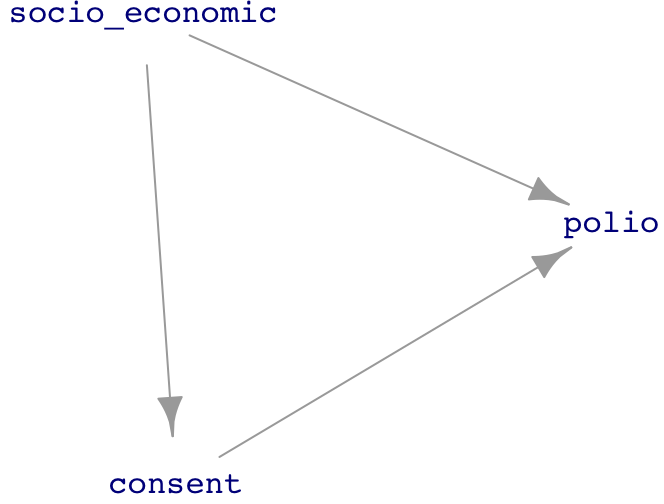
\includegraphics[width=2.21in,height=\textheight]{./www/DAG-consent1.png}

}

\caption{\label{fig-dag-polio}A DAG for the polio vaccine experiment.}

\end{marginfigure}

It is illuminating to look at the vaccine trial as a DAG. The essential
situation is diagrammed in Figure~\ref{fig-dag-polio}. The
\texttt{socio\_economic} node represents the idea that socio-economic
status has an influence on susceptibility to symptomatic
polio\footnote{In contrast to the usual expectation that lower
  socio-economic status is associated higher risk of disease, with polio
  the opposite holds true. The explanation usually given is that
  children who are exposed to the polio virus as infants do not become
  sick but do gain immunity to later infection. People later in
  childhood and in adulthood are at risk of a severe, symptomatic
  response to exposure. Polio is transmitted mainly via a fecal-oral
  route. Conditions favoring this route are more common among those of
  low socio-economic status. Consequently, infants of well-to-do
  families are less exposed to the virus and do not develop immunity.
  When they are eventually exposed to polio as children or adults, the
  well-to-do are at greater risk of developing disease.} and also is a
factor in shaping a family's decision about giving consent.

The DAG in Figure~\ref{fig-dag-polio} has two pathways between
\texttt{treatment} and \texttt{polio} that can produce confounding:

\begin{itemize}
\tightlist
\item
  \(\mathtt{treatment} \leftarrow \mathtt{consent} \rightarrow \mathtt{polio}\)
\item
  \(\mathtt{treatment} \leftarrow \mathtt{consent} \leftarrow \mathtt{socio.economic} \rightarrow \mathtt{polio}\)
\end{itemize}

\begin{marginfigure}

{\centering 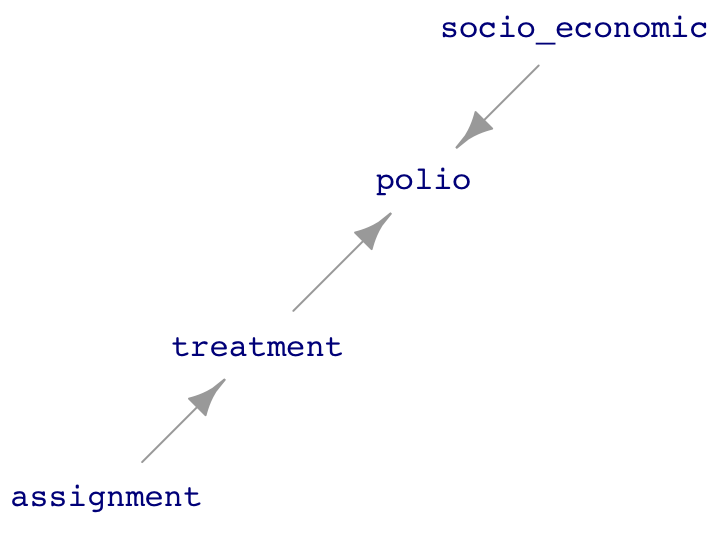
\includegraphics[width=2.37in,height=\textheight]{./www/DAG-consent2.png}

}

\caption{\label{fig-dag-polio-consent}The DAG when \texttt{consent}
\(\equiv\) \texttt{vaccine}.}

\end{marginfigure}

The approach emphasized in Lesson~\ref{sec-lesson-30} to avoid such
confounding is to block the relevant pathways. Both can be blocked by
including \texttt{consent} as a covariate. However, in Study 1,
assignment to vaccine was purely a matter of consent; \texttt{consent}
and \texttt{treatment} are essentially the same variable.
Figure~\ref{fig-dag-polio-consent} shows the corresponding DAG, where
\texttt{consent} and \texttt{treatment} are merged into a single
variable. Holding \texttt{consent} constant deprives the system of the
explanatory variable and still introduces confounding through
\texttt{socio\_economic}.

In Study 2, all the children participating had parents give consent.
This means that \texttt{consent} is not actually a variable; it doesn't
vary! The corresponding DAG, without \texttt{consent} as a factor, is
drawn in Figure~\ref{fig-dag-polio3}. This Study 2 DAG is unfolded;
there are no confounding pathways! Thus the model
\texttt{polio\ \textasciitilde{}\ treatment} is appropriate.

\begin{marginfigure}

{\centering 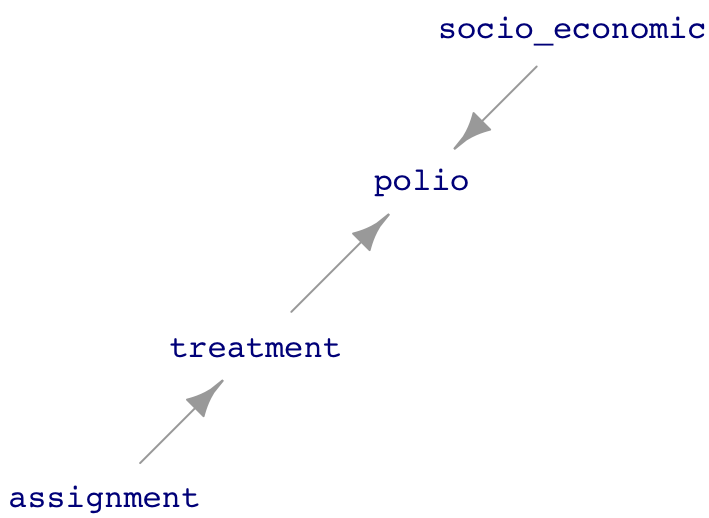
\includegraphics[width=2.36in,height=\textheight]{./www/DAG-consent3.png}

}

\caption{\label{fig-dag-polio3}The Study 2 DAG.}

\end{marginfigure}

The assignment to treatment or control in Figure~\ref{fig-dag-polio3} is
made by the people running the study. Although the DAG doesn't show any
inputs to \texttt{assignment}, the involvement of people in making the
assignment opens up a possibility that their assignment of treatment or
control might have been influenced by other factors, such as
socio-economic status. To guard against this, or even skepticism raised
by the possibility, experimentalists have developed a simple safeguard:
``\textbf{random assignment}.'' In random assignment, assignment is made
by a computer generating random numbers. Nobody believes that the
computer algorithm is influenced by socio-economic status or any other
factor that might be connected to polio in any way.

\begin{tcolorbox}[enhanced jigsaw, colbacktitle=quarto-callout-warning-color!10!white, breakable, opacitybacktitle=0.6, colback=white, left=2mm, arc=.35mm, colframe=quarto-callout-warning-color-frame, coltitle=black, toprule=.15mm, opacityback=0, leftrule=.75mm, bottomtitle=1mm, toptitle=1mm, titlerule=0mm, title=\textcolor{quarto-callout-warning-color}{\faExclamationTriangle}\hspace{0.5em}{Under construction}, rightrule=.15mm, bottomrule=.15mm]

\end{tcolorbox}

\hypertarget{blocking}{%
\section{Blocking}\label{blocking}}

\hypertarget{sec-lesson-33}{%
\chapter{Measuring and accumulating risk}\label{sec-lesson-33}}

The \emph{linear models} (\texttt{lm()}) we have mostly been using up
until now accumulate the model output as a linear combination of model
inputs. Consider, for instance, a simple model of fuel economy based on
the horsepower and weight of a car:

\begin{Shaded}
\begin{Highlighting}[]
\NormalTok{mpg\_mod }\OtherTok{\textless{}{-}} \FunctionTok{lm}\NormalTok{(mpg }\SpecialCharTok{\textasciitilde{}}\NormalTok{ hp }\SpecialCharTok{+}\NormalTok{ wt, }\AttributeTok{data =}\NormalTok{ mtcars) }
\NormalTok{mpg\_mod }\SpecialCharTok{\%\textgreater{}\%} \FunctionTok{coef}\NormalTok{()}
\end{Highlighting}
\end{Shaded}

\begin{verbatim}
(Intercept)          hp          wt 
37.22727012 -0.03177295 -3.87783074 
\end{verbatim}

These coefficients mean that the model output is a \textbf{sum}. For
instance, a 100 horsepower car weighting 2500 pounds has a predicted
fuel economy of \texttt{37.2\ -\ 0.032*100\ -\ 3.88*2.5=}24.3 miles per
gallon.\footnote{The \texttt{wt} variable is measured in units of 1000
  lbs, so a 2500 pound vehicle has a \texttt{wt} value of 2.5.} If we're
interested in making a prediction, we often hide the arithmetic behind a
computer function, but it is the same arithmetic:

\begin{Shaded}
\begin{Highlighting}[]
\FunctionTok{mod\_eval}\NormalTok{(mpg\_mod, }\AttributeTok{hp =} \DecValTok{100}\NormalTok{, }\AttributeTok{wt =} \FloatTok{2.5}\NormalTok{)}
\end{Highlighting}
\end{Shaded}

\ttfamily 
\begin{tabular}{rrr}
\toprule
hp & wt & model\_output\\
\midrule
100 & 2.5 & 24.3554\\
\bottomrule
\end{tabular} \normalfont
\bigskip

The arithmetic, in principle, lets us evaluate the model for any inputs,
even ridiculous ones like a 10,000 hp car weighing 50,000 lbs. There is
no such car, but there is a model output.\footnote{A 10,000 hp, 50,000
  lbs ground vehicle does have a name: a ``tank.'' Common sense dictates
  that one not put too much stake in a calculation of a tank's fuel
  economy based on data from cars!}

\begin{Shaded}
\begin{Highlighting}[]
\FunctionTok{mod\_eval}\NormalTok{(mpg\_mod, }\AttributeTok{hp=}\DecValTok{10000}\NormalTok{, }\AttributeTok{wt =} \DecValTok{50}\NormalTok{)}
\end{Highlighting}
\end{Shaded}

\ttfamily 
\begin{tabular}{rrr}
\toprule
hp & wt & model\_output\\
\midrule
10000 & 50 & -474.3937\\
\bottomrule
\end{tabular} \normalfont
\bigskip

The prediction reported here means that such a car goes \emph{negative}
474 miles on a gallon of gas. That's silly. Fuel economy needs to be
non-negative; the output \(-474\) mpg is \emph{out of bounds}.

A good way to avoid out-of-bounds behavior is to model a
\emph{transformation} of the response variable instead of the variable
itself. For example, to avoid negative outputs from a model of
\texttt{mpg}, change the model so that the output is in terms of the
logarithm of \texttt{mpg}, like this:

\begin{Shaded}
\begin{Highlighting}[]
\NormalTok{logmpg\_mod }\OtherTok{\textless{}{-}} \FunctionTok{lm}\NormalTok{(}\FunctionTok{log}\NormalTok{(mpg) }\SpecialCharTok{\textasciitilde{}}\NormalTok{ hp }\SpecialCharTok{+}\NormalTok{ wt, }\AttributeTok{data =}\NormalTok{ mtcars) }
\FunctionTok{mod\_eval}\NormalTok{(logmpg\_mod, }\AttributeTok{hp =} \DecValTok{100}\NormalTok{, }\AttributeTok{wt =} \FloatTok{2.5}\NormalTok{)}
\end{Highlighting}
\end{Shaded}

\ttfamily 
\begin{tabular}{rrr}
\toprule
hp & wt & model\_output\\
\midrule
100 & 2.5 & 3.173411\\
\bottomrule
\end{tabular} \normalfont
\bigskip

The reported output, 3.17, should \textbf{not} be interpreted as
\texttt{mpg}. Instead, interpret it as \texttt{log(mpg)}. If we want
output in terms of \texttt{mpg}, then we have to undo the logarithm.
That's the role of the exponential function, which is the \emph{inverse}
of the logarithm.

\begin{Shaded}
\begin{Highlighting}[]
\FunctionTok{mod\_eval}\NormalTok{(logmpg\_mod, }\AttributeTok{hp =} \DecValTok{100}\NormalTok{, }\AttributeTok{wt =} \FloatTok{2.5}\NormalTok{) }\SpecialCharTok{\%\textgreater{}\%}
  \FunctionTok{mutate}\NormalTok{(}\AttributeTok{mpg =} \FunctionTok{exp}\NormalTok{(model\_output))}
\end{Highlighting}
\end{Shaded}

\ttfamily 
\begin{tabular}{rrrr}
\toprule
hp & wt & model\_output & mpg\\
\midrule
100 & 2.5 & 3.173411 & 23.88884\\
\bottomrule
\end{tabular} \normalfont
\bigskip

The logarithmic transform at the model-training stage does not not
prevent the model output from being negative. We can see this by looking
at the tank example:

\begin{Shaded}
\begin{Highlighting}[]
\NormalTok{mod\_logmpg }\OtherTok{\textless{}{-}} \FunctionTok{lm}\NormalTok{(}\FunctionTok{log}\NormalTok{(mpg) }\SpecialCharTok{\textasciitilde{}}\NormalTok{ hp }\SpecialCharTok{+}\NormalTok{ wt, }\AttributeTok{data =}\NormalTok{ mtcars)}
\FunctionTok{mod\_eval}\NormalTok{(mod\_logmpg, }\AttributeTok{hp=}\DecValTok{10000}\NormalTok{, }\AttributeTok{wt=}\DecValTok{50}\NormalTok{) }\SpecialCharTok{\%\textgreater{}\%}
  \FunctionTok{mutate}\NormalTok{(}\AttributeTok{mpg =} \FunctionTok{exp}\NormalTok{(model\_output))}
\end{Highlighting}
\end{Shaded}

\ttfamily 
\begin{tabular}{rrrr}
\toprule
hp & wt & model\_output & mpg\\
\midrule
10000 & 50 & -21.6327 & 0\\
\bottomrule
\end{tabular} \normalfont
\bigskip

The model output is negative for the tank, but the model output
corresponds to \texttt{log(mpg)}. What will keep the model from
producing negative \texttt{mpg} will be the exponential transformation
applied to the model output. A graph of the exponential function shows
how this works.

\begin{figure}

\sidecaption{\label{fig-log-mpg}The exponential function translates
\texttt{log(mpg)}, which can be positive or negative, into \texttt{mpg},
which can only be non-negative.}

{\centering 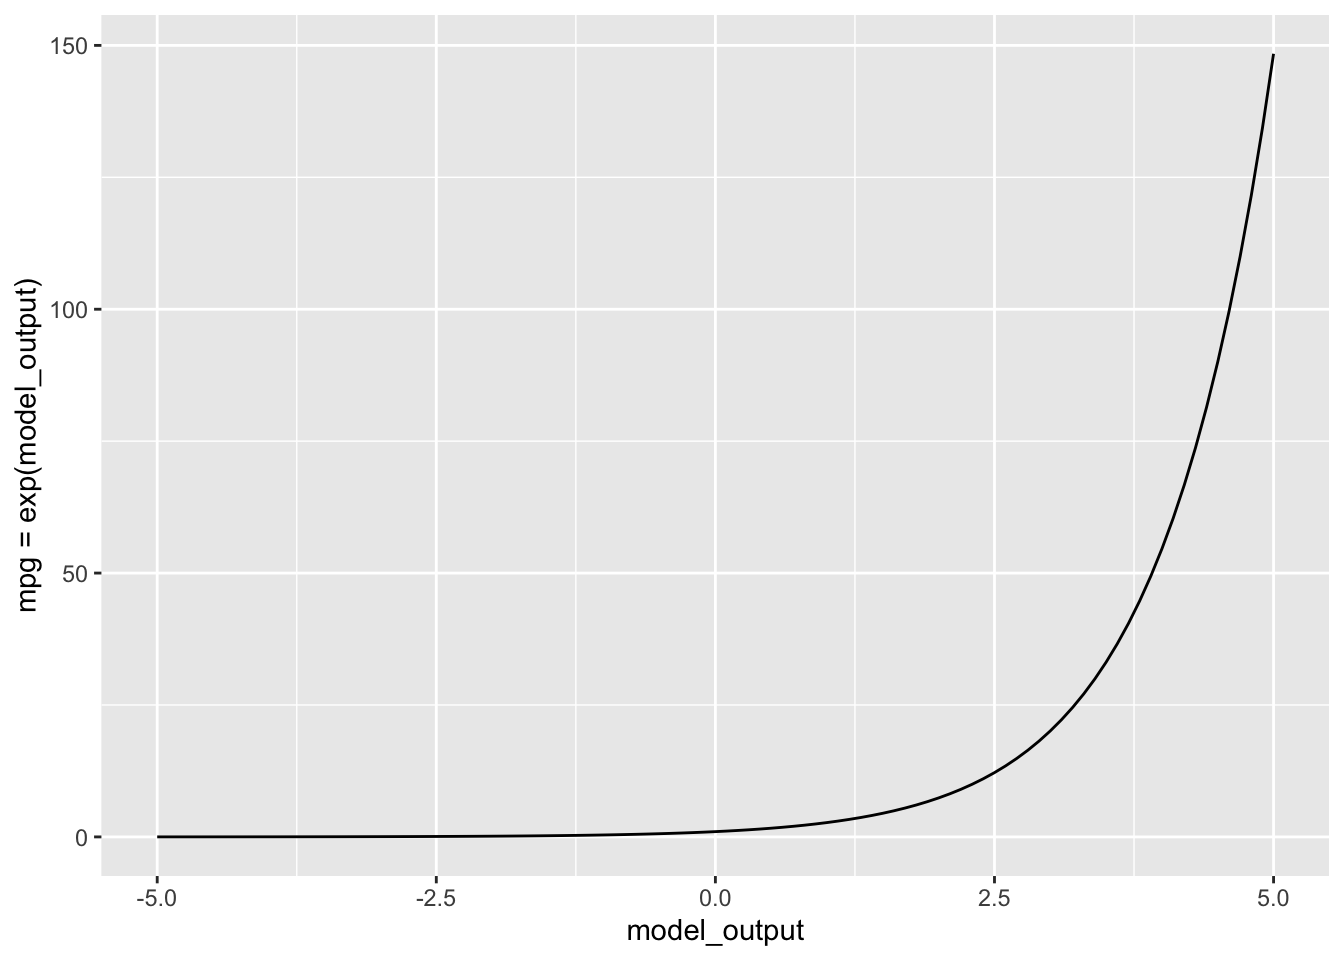
\includegraphics{./Reading-notes-lesson-33_files/figure-pdf/fig-log-mpg-1.pdf}

}

\end{figure}

The log transform does not fix the absurdity of modeling tanks based on
the fuel economy of cars. The model's prediction of \texttt{mpg} for the
tank is 0.0000000004 miles/gallon, but real-world tanks do much better
than that. For instance, the M1 Abrams tank is reported to get
approximately 0.6 miles per gallon.

\hypertarget{risk}{%
\section{Risk}\label{risk}}

In everyday language, ``risk'' refers to a dangerous or unwelcome
outcome. We talk about the ``risk of heart disease'' or the ``risk of
bankruptcy'' or other financial loss. To apply risk to a positive
outcome is non-idiomatic. For instance, for a person wanting to have a
baby, we don't talk about the ``risk of pregnancy,'' but about the
``chances of becoming pregnant.''

In statistics, the word ``risk'' is similarly used for an unwelcome
outcome. However, an additional component of meaning is added. ``Risk''
refers to the \textbf{probability} of the unwelcome outcome. In
principle, though, it would be entirely equivalent to speak of the
``probability of heart disease,'' leaving the phrase ``heart disease''
to signal that the outcome is unwanted. We talk about the ``risk of
death'' but never the ``risk of survival.'' Instead, we would say
something like the ``chances of survival.''

The outcomes described by ``risk'' are categorical. Generically, the
levels of the categorical variable might be ``unwelcome'' and ``not
unwelcome,'' but they might be more specifically named, say, ``death''
and ``survival,'' or ``lung disease'' and ``not.''

We have been building models of such categorical output variables from
the start of these Lessons. For the zero-one categorical variables we
have emphasized, the model output is in the form of a probability: the
probability of the outcome of the event being ``one'' (or whatever
actual level ``one'' corresponds to.) If we assign one for ``death'' and
zero for ``survival,'' the probability which is the output of a model is
a risk, but other than the choice of zero-one assignment, there is no
mathematical difference (in statistics) between a risk and a
probability.

It often happens that risk depends on other factors, often called ``risk
factors.'' In our modeling framework, such risk factors are merely
explanatory variables. For instance, a study of the impact of smoking on
health might use \texttt{outcome} represented by a categorical response
variable with levels ``death'' or ``survival.''

To summarize, for statistical thinkers a model of risk takes the usual
form that we have used for models of zero-one categorical models. All
the same issues apply: covariates, DAGs, confidence intervals, and so
on. There is, however, a slightly different style for presenting effect
sizes.

Up until now, we have presented effect in terms of an arithmetic
difference. As an example, we turn to the fuel-economy model introduced
at the beginning of this lesson. Effect sizes are about \emph{changes}.
To look at the effect size of, say, weight (\texttt{wt}), we would
calculate the model output for two cars that differ in weight (but are
the same for the other explanatory variables). For instance, to know the
change in fuel economy due to a 1000 pound change in weight, we can do
this calculation:

\begin{Shaded}
\begin{Highlighting}[]
\FunctionTok{mod\_eval}\NormalTok{(logmpg\_mod, }\AttributeTok{hp =} \DecValTok{100}\NormalTok{, }\AttributeTok{wt =} \FunctionTok{c}\NormalTok{(}\FloatTok{2.5}\NormalTok{, }\FloatTok{3.5}\NormalTok{)) }\SpecialCharTok{\%\textgreater{}\%}
  \FunctionTok{mutate}\NormalTok{(}\AttributeTok{mpg =} \FunctionTok{exp}\NormalTok{(model\_output))}
\end{Highlighting}
\end{Shaded}

\ttfamily 
\begin{tabular}{rrrr}
\toprule
hp & wt & model\_output & mpg\\
\midrule
100 & 2.5 & 3.173411 & 23.88884\\
100 & 3.5 & 2.972875 & 19.54803\\
\bottomrule
\end{tabular} \normalfont
\bigskip

The lighter car is predicted to get 24 mpg, the heavier car to get 19.5
mpg. The arithmetic difference in output \(19.5 - 24 = -4.5\) mpg is the
effect of the 1000 pound increase in weight.

There is another way to present the effect, as a \textbf{ratio} or
proportion. In this style, the effect of an addition 1000 pounds is
\(19.5 / 24 = 81\%\), that is, the heavier car can go only 81\% of the
distance that the lighter car will travel on the same amount of
gasoline. (Stating an effect as a ratio is common in some fields. For
example, economists use ratios when describing prices or investment
returns.)

In presenting a change in risk---that is, the change in probability
resulting from a change in some explanatory variable---both the
arithmetic difference and arithmetic ratio forms are used. But there is
a special terminology that is used to identify the two forms. A change
in the form of an arithmetic difference is called an ``\textbf{absolute}
change in risk.'' A change in the ratio form is called a
``\textbf{relative} risk.''

The different forms---absolute change in risk versus relative
risk---both describe the same change in risk. For most decision-makers,
the absolute form is most useful. To illustate, suppose exposure to a
toxin increases the risk of a disease by 50\%. This would be a risk
ratio of 1.5. But that risk ratio might be based on an absolute change
in risk from 0.00004 to 0.00006, or it might be based on an absolute
change in risk from 40\% to 60\%. The latter is a much more substantial
change in risk and ought to warrant more attention from decision makers
interested.

\begin{tcolorbox}[enhanced jigsaw, colbacktitle=quarto-callout-note-color!10!white, breakable, opacitybacktitle=0.6, colback=white, left=2mm, arc=.35mm, colframe=quarto-callout-note-color-frame, coltitle=black, toprule=.15mm, opacityback=0, leftrule=.75mm, bottomtitle=1mm, toptitle=1mm, titlerule=0mm, title=\textcolor{quarto-callout-note-color}{\faInfo}\hspace{0.5em}{Other ways to measure change in risk}, rightrule=.15mm, bottomrule=.15mm]

It is important for measures of change in risk to be mathematically
valid. But from among the mathematically valid measures, one wants to
choose a form that will be the best for communicating with
decision-makers. Those decision-makers might be the people in charge of
establishing screening for diseases like breast cancer, or a judge and
jury deciding the extent to which blame for an illness ought to be
assigned to second-hand smoke.

Two useful ways to present a change in risk are the ``\textbf{number
needed to treat}'' (NNT) and the ``\textbf{attributable fraction}.'' The
NNT is useful for presenting the possible benefits of a treatment or
screening test. Consider these data from the
\href{https://www.uspreventiveservicestaskforce.org/uspstf/document/RecommendationStatementFinal/breast-cancer-screening}{US
Preventive Services Task Force} which take the form of the number of
breast-cancer deaths in a 10-year period avoided by mammography. The
confidence interval on the estimated number is also given.

\begin{longtable}[]{@{}lll@{}}
\toprule()
Age & Deaths avoided & Conf. interval \\
\midrule()
\endhead
40-49 & 3 & 0-9 \\
50-59 & 8 & 2-17 \\
60-69 & 21 & 11-32 \\
70-74 & 13 & 0-32 \\
\bottomrule()
\end{longtable}

The table does not give the risk of death, but rather the absolute risk
reduction. For the 70-74 age group this risk reduction is 13/100000 with
a confidence interval of 0 to 32/100000.

The NNT is well named. It gives the number of people who must receive
the treatment in order to avoid one death. Arithmetically, the NNT is
simply the reciprocal of the absolute risk reduction. So, for the 70-74
age group the NNT is 100000/13 or 7700 or, stated as a confidence
interval, {[}3125 to \(\infty\){]}.

For a decision-maker, NNT presents the effect size in a readily
understood way. For example, the 40-49 year-old group has an NTT of
33,000. The cost of the treatment could be presented in terms of anxiety
prevented (mammography produces a lot of false positives) or monetary
cost. The US Affordable Care Act requires health plans to fully cover
the cost of a screening mammogram every one or two years for women over
40. Those mammograms each cost about \$100-200. Consequently, the cost
of mammography over the ten-year period (during which 5 mammograms might
be performed) is roughly \(5\times \$100 \times 33000\) or about \$16
million per life saved.

The attributable fraction is a way of presenting a risk ratio---in other
words, a relative risk---in a way that is more concrete than the ratio
itself. Consider the effect of smoking on the risk of getting lung
cancer. According to the
\href{https://www.cdc.gov/cancer/lung/basic_info/risk_factors.htm\#:~:text=People\%20who\%20smoke\%20cigarettes\%20are,the\%20risk\%20of\%20lung\%20cancer.}{US
Centers for Disease Control}, ``People who smoke cigarettes are 15 to 30
times more likely to get lung cancer.'' This statement directly gives
the confidence interval on the relative risk: {[}15 to 30{]}.

The attributable fraction refers to the proportion of disease in the
exposed group---that is, smokers---to be attributed to expose. The
general formula for attributable fraction is simple. If the risk ratio
is denoted \(RR\), the attributable fraction is
\[\text{attributable fraction} \equiv \frac{RR-1}{RR}\] For a smoker who
gets lung cancer, the confidence interval on the attributable fraction
is {[}93\% to 97\%{]}.

For second-hand smoke, the CDC estimates the risk ratio for cancer at
{[}1.2 to 1.3{]}. For a person exposed to second-hand smoke who gets
cancer, the attributable fraction is {[}17\% to 23\%{]}. Such
attributions are useful for those, such as judges and juries, who need
to assign a level of blame for a bad outcome.

\end{tcolorbox}

\hypertarget{accumulating-risk}{%
\section{Accumulating risk}\label{accumulating-risk}}

There can be multiple factors that contribute to risk. As a simple
example of how different factors can contribute simultaneously, consider
the following DAG:

\begin{Shaded}
\begin{Highlighting}[]
\FunctionTok{dag\_draw}\NormalTok{(dag09)}
\end{Highlighting}
\end{Shaded}

\begin{marginfigure}

{\centering 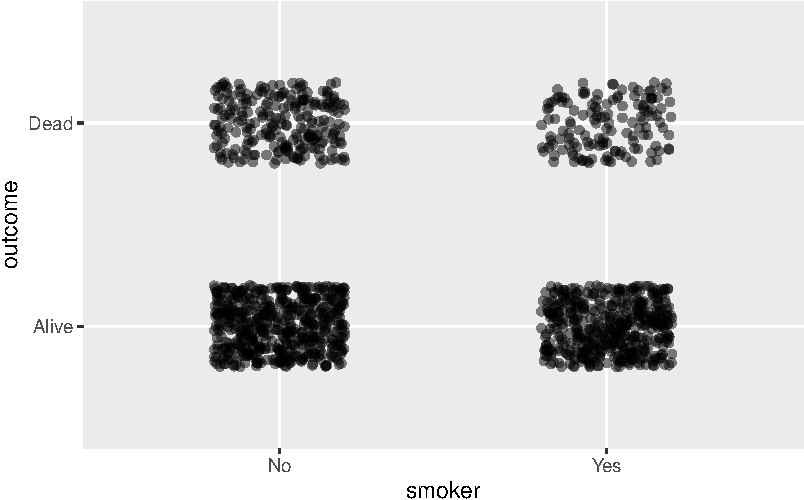
\includegraphics{./Reading-notes-lesson-33_files/figure-pdf/unnamed-chunk-9-1.pdf}

}

\end{marginfigure}

\begin{Shaded}
\begin{Highlighting}[]
\FunctionTok{print}\NormalTok{(dag09)}
\end{Highlighting}
\end{Shaded}

\begin{verbatim}
a ~ exo()
b ~ exo()
c ~ binom(2 * a + 3 * b)
\end{verbatim}

The formulas for \texttt{dag09} show that the nodes \texttt{a} and
\texttt{b} are exogenous, their values set randomly and independently of
one another by the \texttt{exo()} function. Both \texttt{a} and
\texttt{b} contribute to the value of \texttt{c}. Ordinary stuff. But
there is something new in this simulation, the \texttt{binom()}
function. The output of \texttt{binom()} will always be either 0 or 1.
If the input to \texttt{binom()} is zero, it's completely random whether
a 0 or 1 will result. The more positive the input to \texttt{binom()},
the larger the chance of a 1. Similarly, the more negative the input,
the larger the chance of a 0. Like this:

\begin{verbatim}

Attaching package: 'mosaicCalc'
\end{verbatim}

\begin{verbatim}
The following object is masked from 'package:mosaicModel':

    Runners
\end{verbatim}

\begin{verbatim}
The following object is masked from 'package:stats':

    D
\end{verbatim}

\begin{figure}

\sidecaption{\label{fig-binom-fun-1}The \texttt{binom()} function looks
to its input to determine the probability that the output will be 1 or
0.}

{\centering 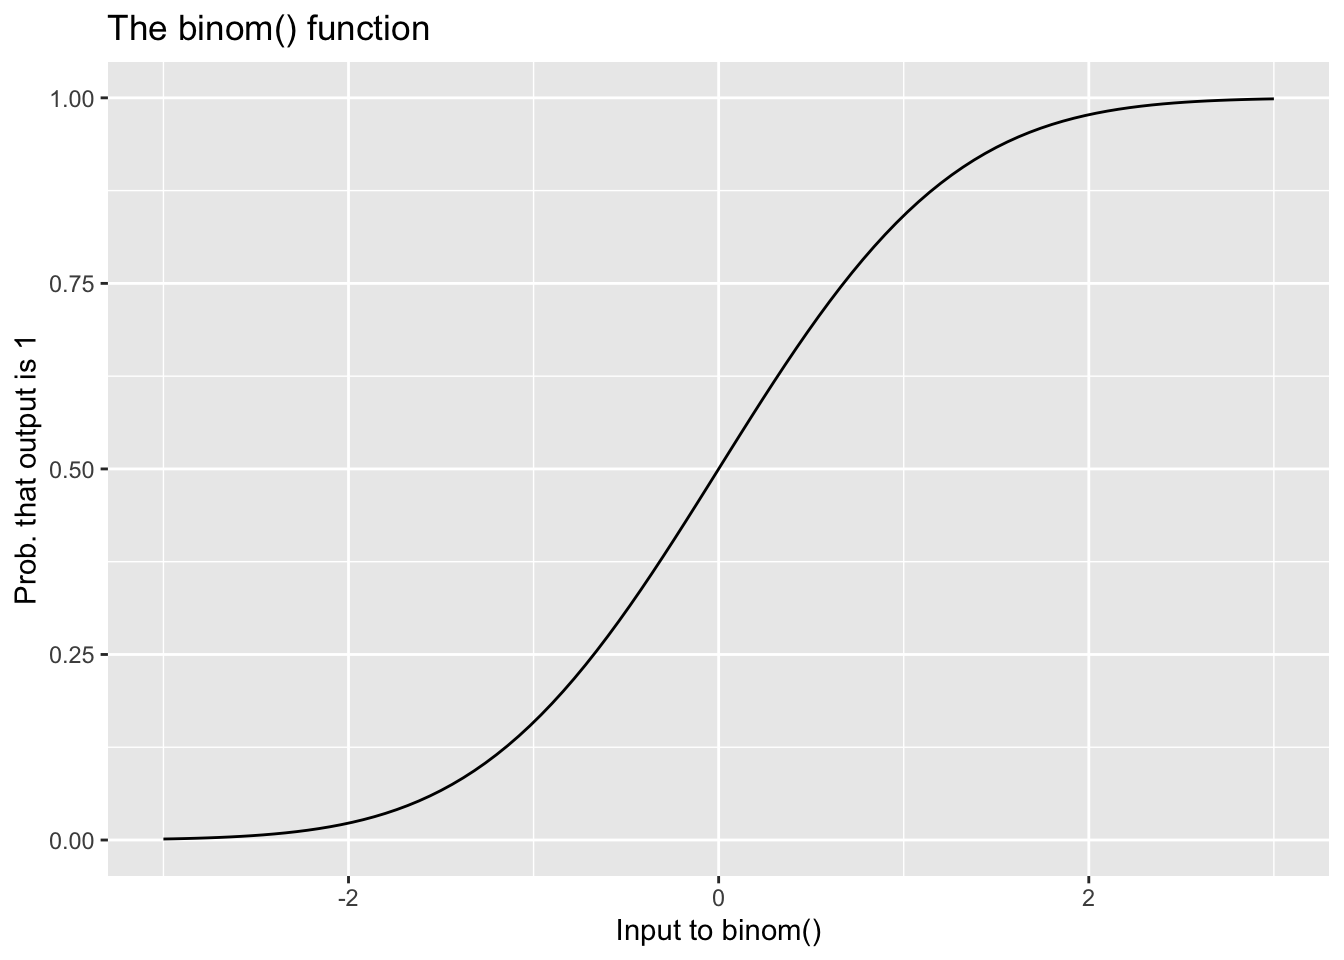
\includegraphics{./Reading-notes-lesson-33_files/figure-pdf/fig-binom-fun-1-1.pdf}

}

\end{figure}

In \texttt{dag09}, the input to \texttt{binom()} is
\texttt{2*a\ +\ 3*b}; both \texttt{a} and \texttt{b} are risk factors
for \texttt{c} being 1. The larger that \texttt{a} is, the larger the
risk. Similarly, the larger \texttt{b}, the larger the risk. The formula
\texttt{2*a\ +\ 3*b} accumulates the risk steming from \texttt{a} and
\texttt{b}.

Let's generate a big sample---\(n=10,000\)---from \texttt{dag09} and see
if a simple model is able to capture the way \texttt{a} and \texttt{b}
contribute to \texttt{c}:

\begin{Shaded}
\begin{Highlighting}[]
\FunctionTok{sample}\NormalTok{(dag09, }\AttributeTok{size=}\DecValTok{10000}\NormalTok{) }\SpecialCharTok{\%\textgreater{}\%} 
  \FunctionTok{lm}\NormalTok{(c }\SpecialCharTok{\textasciitilde{}}\NormalTok{ a }\SpecialCharTok{+}\NormalTok{ b, }\AttributeTok{data =}\NormalTok{ .) }\SpecialCharTok{\%\textgreater{}\%}
  \FunctionTok{conf\_interval}\NormalTok{()}
\end{Highlighting}
\end{Shaded}

\ttfamily 
\begin{tabular}{lrr}
\toprule
term & .lwr & .upr\\
\midrule
(Intercept) & 0.4869220 & 0.5005108\\
a & 0.1951406 & 0.2087079\\
b & 0.2922837 & 0.3058925\\
\bottomrule
\end{tabular} \normalfont
\bigskip

The coefficients on \texttt{a} and \texttt{b} are inconsistent with the
\texttt{dag09} formulas. What's wrong? The problem can be seen in
Figure~\ref{fig-binom-fun-1}. The output of \texttt{binom()} is a
probability. Probabilities have to stay within the bounds 0 to 1. But
there is nothing in the formula \texttt{c\ \textasciitilde{}\ a\ +\ b}
that enforces such bounds. If we are to model zero-one response
variables like \texttt{c}, we will need a means to enforce the bounds.

\hypertarget{probability-odds-and-log-odds}{%
\section{Probability, odds, and log
odds}\label{probability-odds-and-log-odds}}

\begin{tcolorbox}[enhanced jigsaw, colbacktitle=quarto-callout-warning-color!10!white, breakable, opacitybacktitle=0.6, colback=white, left=2mm, arc=.35mm, colframe=quarto-callout-warning-color-frame, coltitle=black, toprule=.15mm, opacityback=0, leftrule=.75mm, bottomtitle=1mm, toptitle=1mm, titlerule=0mm, title=\textcolor{quarto-callout-warning-color}{\faExclamationTriangle}\hspace{0.5em}{Under construction}, rightrule=.15mm, bottomrule=.15mm]

\end{tcolorbox}

A probability---a number between 0 and 1---is the most used measure of
the chances that something will happen, but it is not the only way nor
the best for all purposes.

Also part of everyday language is the word ``odds,'' as in, ``What are
the odds?'' to express surprise at an unexpected event.

Odds are usually expressed in terms of two numbers, as in ``3 to 2'' or
``100 to 1'', written more compactly as 3:2 and 100:1 or even 1.5 and
100, respectively. The setting for odds is an even that might happen or
not: the horse Fortune's Chance might win the race, otherwise not; it
might rain today, otherwise not; the Red Sox might win the World Series,
otherwise not.

The format of a \emph{probability} assigns a number between 0 and 1 to
the chances that Fortune's Chance will win, or that it will rain, or
that the Red Sox will come out on top. If that number is called \(p\),
then the chances of the ``otherwise outcome'' must be \(1-p\). The event
with probability \(p\) would be reformatted into odds as \(p:(1-p)\). No
information is lost if we treat the odds as a single number, the result
of the division \(p/(1-p)\). Thus, when \(p=0.25\) the corresponding
odds will be \(0.25/0.75\), in other words, 1/3.

A big mathematical advantage to using odds is that the odds number can
be anything from zero to infinity; it's not bounded within 0 to 1. Even
more advantageous for the purposes of accumulating risk is the logarithm
of the odds, called ``\textbf{log odds}.'' We will come back to this
later.

The printed version of \texttt{dag09} shows that the value of node
\texttt{c} is a linear combination of \texttt{a} and \texttt{b}
converted into a zero-one, binomial value. Unfortunately, the linear
modeling trainer, \texttt{lm()}, is not well-tuned to work with binomial
data. Another modeling technique, ``logistic regression,'' does a better
job. The \texttt{glm()} function trains logistic regression models on
data.

\begin{Shaded}
\begin{Highlighting}[]
\FunctionTok{sample}\NormalTok{(dag09, }\AttributeTok{size=}\DecValTok{10000}\NormalTok{) }\SpecialCharTok{\%\textgreater{}\%} 
  \FunctionTok{glm}\NormalTok{(c }\SpecialCharTok{\textasciitilde{}}\NormalTok{ a }\SpecialCharTok{+}\NormalTok{ b, }\AttributeTok{data =}\NormalTok{ ., }\AttributeTok{family=}\StringTok{"binomial"}\NormalTok{) }\SpecialCharTok{\%\textgreater{}\%}
  \FunctionTok{conf\_interval}\NormalTok{()}
\end{Highlighting}
\end{Shaded}

\ttfamily 
\begin{tabular}{lrr}
\toprule
term & .lwr & .upr\\
\midrule
(Intercept) & -0.0265355 & 0.0983073\\
a & 1.9339670 & 2.1291936\\
b & 2.9184181 & 3.1726524\\
\bottomrule
\end{tabular} \normalfont
\bigskip

When we use the appropriate modeling technique, we can, in this case,
recover the coefficients in the DAG formula: 2 for \texttt{a} and 3 for
\texttt{b}.

\end{footnotesize}}

\hypertarget{sec-lesson-34}{%
\chapter{Constructing a classifier}\label{sec-lesson-34}}

\[\newcommand{\Ptest}{\mathbb{P}}
\newcommand{\Ntest}{\mathbb{N}}
\newcommand{\given}{\ |\!\!|\  }\]

There are many yes-or-no conditions. A patient has a disease or does
not. A credit-card transaction is genuine or fraudulent.

But it is not always straightforward to figure out at the time the
patient comes to the clinic or the credit-card transaction is made,
whether the condition is yes or no. If we could wait, the condition
might reveal itself: the patient gets critically ill or the credit-hard
holder complains about an unauthorized charge. But we can't wait. We
want to treat the patient \emph{before} he or she gets critically
ill.~We want to block the credit-card transaction before it is
completed.

Instead of waiting, we measure whatever relevant variables we can when
the patient arrives at the clinic or the credit-card transaction has
been submitted for approval. For the patient, we might look at the
concentration of specific markers for cancer in the blood. For the
transaction, we might look at the shipping address to see if it matches
the credit-card holder's genuine address. Such variables may provide an
indication, imperfect though it may be, of whether the condition is yes
or no.

A \textbf{classifier} is a statistical model used to \emph{predict} the
unknown outcome of a yes-or-no situation from information that is
already available. This Lesson concerns three closely related topics
about classifiers: how we collect data for training the model, how we
summarize the performance of the classifier, and how we ``tune'' the
classifier.

\hypertarget{identifying-cases}{%
\section{Identifying cases}\label{identifying-cases}}

Consider this news report and note the time lag between collection of
the dietary explanatory variables and the response variable---whether
the patient developed pancreatic cancer.

\begin{quote}
Higher vitamin D intake has been associated with a significantly reduced
risk of pancreatic cancer, according to a study released last week.
Researchers combined data from two prospective studies that included
46,771 men ages 40 to 75 and 75,427 women ages 38 to 65. They identified
365 cases of pancreatic cancer over 16 years. Before their cancer was
detected, subjects filled out dietary questionnaires, including
information on vitamin supplements, and researchers calculated vitamin D
intake. After statistically adjusting\footnote{That is, applying the
  methods of Lesson~\ref{sec-lesson-28}.} for age, smoking, level of
physical activity, intake of calcium and retinol and other factors, the
association between vitamin D intake and reduced risk of pancreatic
cancer was still significant. Compared with people who consumed less
than 150 units of vitamin D a day, those who consumed more than 600
units reduced their risk by 41 percent. - \emph{New York Times}, 19
Sept.~2006, p.~D6.
\end{quote}

This was not an experiment; it was an observational study without any
intervention to change anyone's diet.

\hypertarget{the-training-sample}{%
\section{The training sample}\label{the-training-sample}}

In building a classifier, we have a similar situation. Perhaps we can
perform the blood test today, but that gives us only the test result,
not the subject's true condition. We might have to wait years for that
condition to reveal itself. Only at that point can we measure the
performance of the classifier.

To picture the situation, let's imagine many people enrolled in the
study, some of whom have the condition and some who don't. On Day 1 of
the study, we test everyone and get raw score on a scale from 0 to 40.
The results are shown in Figure~\ref{fig-case-control}. Each glyph is a
person. The varying locations are meant to help us later on; for now,
just think of them as representing where each person lives in the world.
The different shapes of glyph---circle, square, triangle---are meant to
remind you that people are different from one another in age, gender,
risk-factors, etc.

Each person took a blood test. The raw result from that test is a score
from 0 to 40. The distribution of scores is shown in the right panel of
the figure. We also show the score in the world-plot; the higher the raw
score, the more blue the glyph. On Day 1, it isn't known who has the
condition and who does not.

\begin{figure}

\sidecaption{\label{fig-case-control}Day 1: The people participating in
the study to develop the classifier. Each has been given a blood test
which gives a score from zero (gray) to forty (blue).}

{\centering 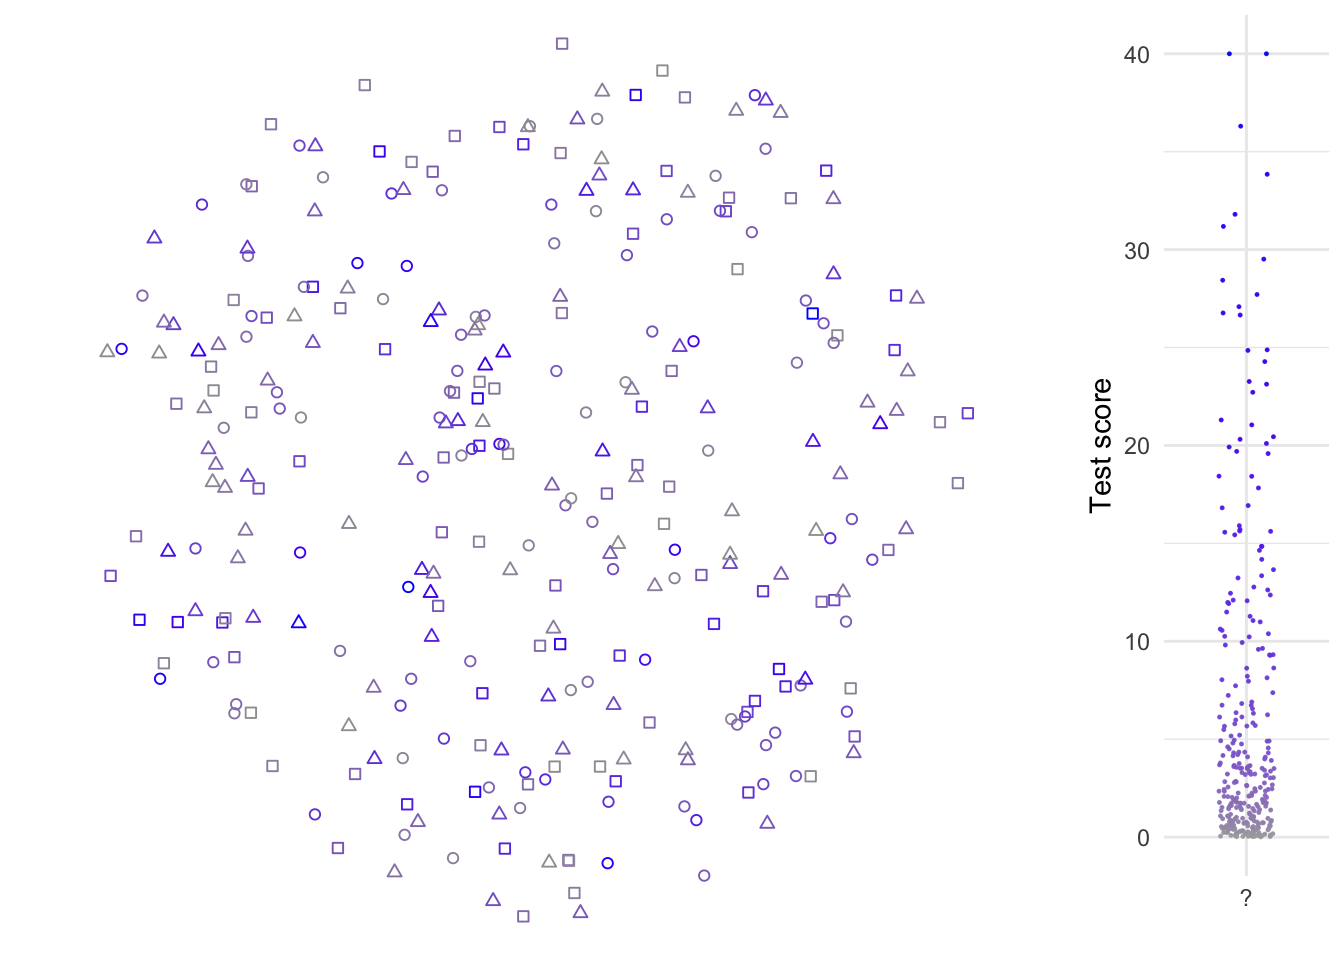
\includegraphics{./Reading-notes-lesson-34_files/figure-pdf/fig-case-control-1.pdf}

}

\end{figure}

Having recorded the raw test results for each person, we wait. In the
pancreatic cancer study, they waited 16 years for the cancer to reveal
itself.

\ldots{} waiting \ldots{}

After the waiting period, we can add a new column to the original data;
whether the person has the condition (C) or doesn't (H).

Figure~\ref{fig-compare-scores} shows the distribution of raw test
scores for the C group and the H group. The scores are those recorded on
Day 1, but after waiting to find out the patients' conditions, we can
subdivide them into those who have the condition (C) and those who don't
(H).

\begin{figure}

\sidecaption{\label{fig-compare-scores}The distribution of raw test
scores. After we know the true condition, we can break down the test
scores by condition.}

{\centering 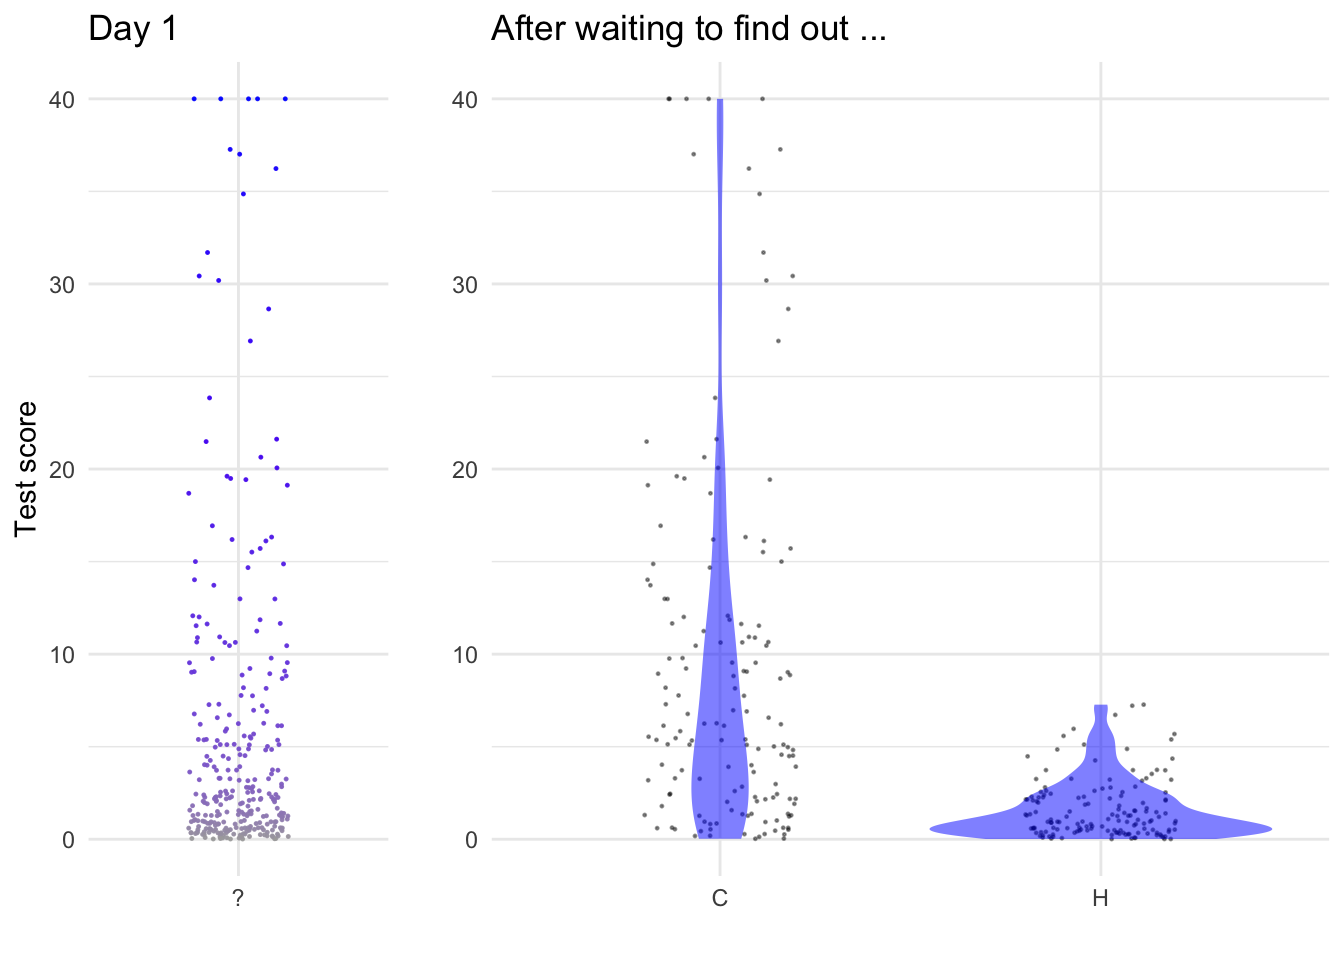
\includegraphics{./Reading-notes-lesson-34_files/figure-pdf/fig-compare-scores-1.pdf}

}

\end{figure}

\hypertarget{applying-a-threshold}{%
\section{Applying a threshold}\label{applying-a-threshold}}

To finish the classifier, we need to identify a ``\textbf{threshold
score}.'' Raw scores above this threshold will generate a
\({\mathbb{P}}\) test; scores below the threshold generate a
\({\mathbb{N}}\) test.

We can make a good guess at an appropriate threshold score from the
presentation in the right panel of Figure~\ref{fig-compare-scores}. The
objective in setting the threshold is to distinguish the C group from
the H group. Setting the threshold at a score around 3 does a pretty
good job.

It helps to give names to the two test results: \({\mathbb{P}}\) and
\({\mathbb{N}}\). Anyone with a score above 3 has result
\({\mathbb{P}}\), anyone with a score below 3 has an \({\mathbb{N}}\)
result.

\begin{figure}

{\centering 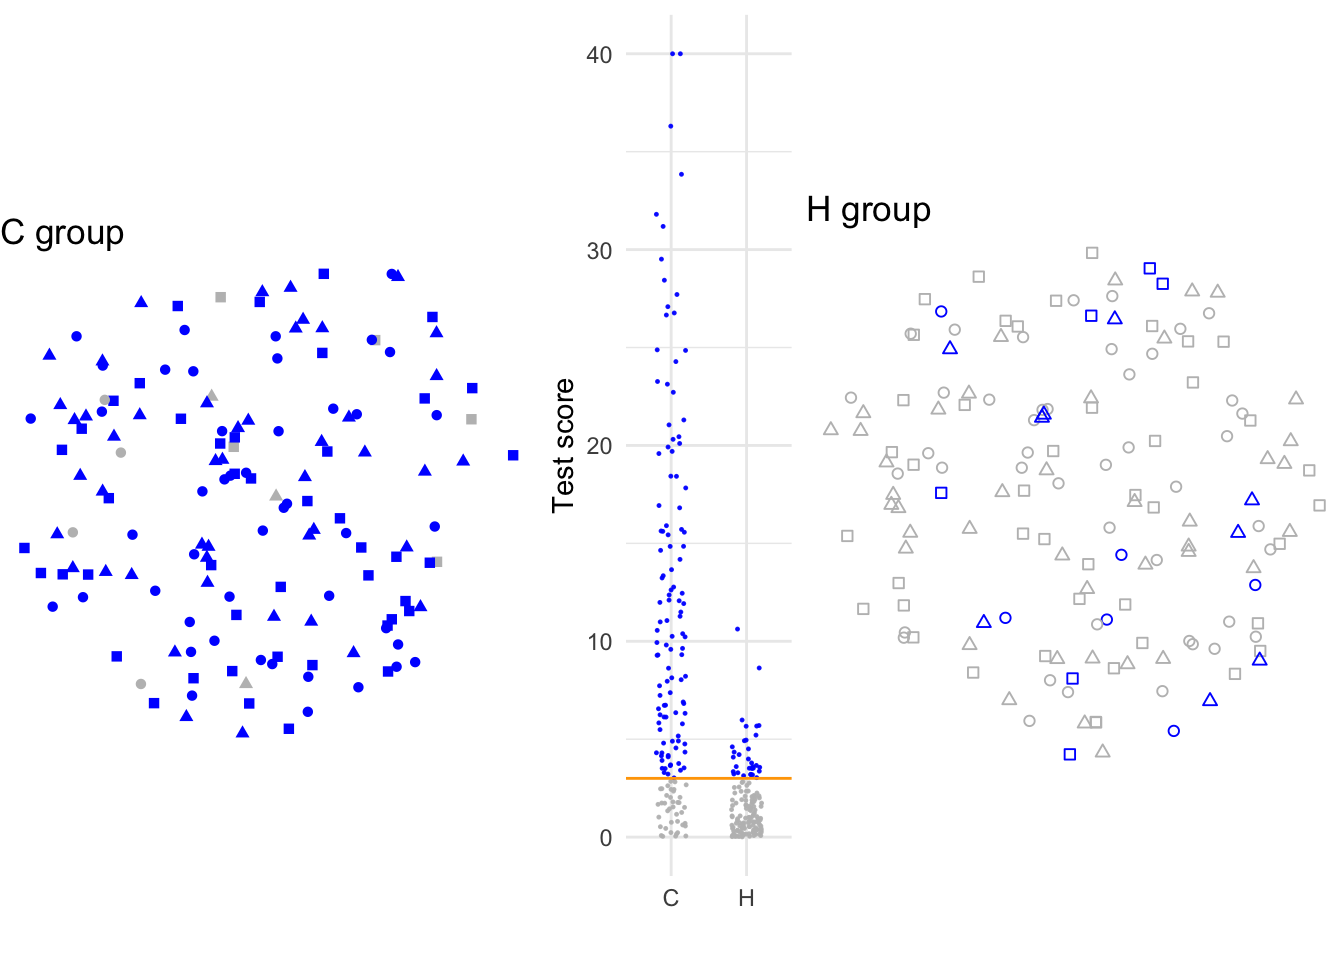
\includegraphics{./Reading-notes-lesson-34_files/figure-pdf/fig-divided-by-condition-1.pdf}

}

\caption{\label{fig-divided-by-condition}Blue is a \(\mathbb{P}\)
result, gray a \(\mathbb{N}\) result.}

\end{figure}

\hypertarget{false-positives-and-false-negatives}{%
\section{False positives and false
negatives}\label{false-positives-and-false-negatives}}

NARRATE Figure~\ref{fig-divided-by-condition} to point out the gray dots
in the C group and the blue dots in the H group. These are errors. But
there are two kinds of errors.

\begin{itemize}
\item
  False-positive: blue dots in the H group. The ``positive'' refers to
  the \({\mathbb{P}}\) test result, the ``false'' simply means the test
  result was wrong.
\item
  False-negative: gray dots in the C group. The ``negative'' refers to
  the \({\mathbb{N}}\) result. Again, the ``false'' means simply that
  the test result is out of line with the actual condition of the
  person.
\end{itemize}

In the training sample shown in Figure~\ref{fig-divided-by-condition},
there are 300 people altogether and 17 false-negatives. This gives a
false-negative rate of about 6\%. Similarly there are 30
false-negatives, a false-positive rate of 10\%.

\begin{tcolorbox}[enhanced jigsaw, colbacktitle=quarto-callout-note-color!10!white, breakable, opacitybacktitle=0.6, colback=white, left=2mm, arc=.35mm, colframe=quarto-callout-note-color-frame, coltitle=black, toprule=.15mm, opacityback=0, leftrule=.75mm, bottomtitle=1mm, toptitle=1mm, titlerule=0mm, title=\textcolor{quarto-callout-note-color}{\faInfo}\hspace{0.5em}{Feature engineering: selling dog food}, rightrule=.15mm, bottomrule=.15mm]

Naturally, the objective when building a classifier is to avoid errors.
One way to avoid errors is by careful ``\textbf{feature engineering}.''
Here, ``features'' refers to the inputs to the classifier model. Often,
the designer of the classifier has multiple variables (``features'') to
work with. (See example.) Choosing a good set of features can be the
difference between a successful classifier and one that makes so many
mistakes as to be useless.

We will use the name ``Bullseye'' to refer to a major, national, big-box
retailing chain which sells, among many other products, dog food. Sales
are largely determined by customer habits; people tend to buy where and
what they have previously bought. There are many places to buy dog food,
for instance pet supermarkets and grocery stores.

One strategy for increasing sales involves discount coupons. A steep
discount provides a consumer incentive to try something new and, maybe,
leads to consumers forming new habits. But, from a sales perspective,
there is little point in providing discounts to people who already have
the habit of buying dog food from the retailer. Instead, it is most
efficient to provide the discount only to people who don't yet have that
habit

The Bullseye marketing staff decided to build a classifier to identify
pet owners who already shop at Bullseye but do not purchase dog food
there. The data available, from Bullseye's ``loyalty'' program,
consisted of individual customers' past purchases of the tens of
thousands of products sold at Bullseye.

Which of these many products to use as indicators of a customer's
potential to switch to Bullseye's dog food? This is where feature
engineering comes in. Searching through Bullseye's huge database, the
feature engineers identified that customers who buy dog food also buy
carpet cleaner. But many people buy carpet cleaner who don't buy dog
food. The engineers searched for purchases might distinguish dog owners
from other users of carpet cleaner.

The feature engineers' conclusion: Send dog-food coupons to people who
buy carpet cleaner but do not buy diapers. Admittedly, this will leave
out the people who have both dogs and babies: these are false negatives.
It will also lead to coupons being sent to petless, spill-prone people
whose children, if any, have moved beyond diapers: false-positives.

\end{tcolorbox}

\hypertarget{threshold-sensitivity-and-specificity}{%
\section{Threshold, sensitivity and
specificity}\label{threshold-sensitivity-and-specificity}}

In Figure~\ref{fig-divided-by-condition} the threshold between
\({\mathbb{P}}\) and \({\mathbb{N}}\) is set at a score of 3. That might
have been a good choice, but it pays to take a more careful look.

That graph is hard to read because the scores have a very long-tailed
distribution; the large majority of scores are below 2 but the scores go
up to 40. To make it easier to compare scores between the C and H
groups, Figure~\ref{fig-compare-scores2} shows the scores on a nonlinear
axis. Each score is marked as a letter: ``P'' means \({\mathbb{P}}\),
``N'' means \({\mathbb{N}}\). False results are colored red.

\begin{Shaded}
\begin{Highlighting}[]
\DocumentationTok{\#\# PNplot(threshold=3)}
\NormalTok{knitr}\SpecialCharTok{::}\FunctionTok{include\_graphics}\NormalTok{(}\StringTok{"www/PN{-}threshold1.png"}\NormalTok{)}
\end{Highlighting}
\end{Shaded}

\begin{figure}[H]

\sidecaption{\label{fig-compare-scores2}Redrawing the participants'
scores from Figure~\ref{fig-compare-scores} on a nonlinear axis. Color
marks whether the classifier gave a correct output.}

{\centering \includegraphics[width=4.48in,height=\textheight]{./www/PN-threshold1.png}

}

\end{figure}

Moving the threshold up would reduce the number of false-positives. At
the same time, the larger threshold would \emph{increase} the number of
false-negatives. \textbf{?@fig-two-thresholds} shows what the situation
would be if the threshold had been set at, say, 10 or 0.5.

\begin{marginfigure}

{\centering \includegraphics[width=4.48in,height=\textheight]{./www/PN-threshold1.png}

}

\caption{\label{fig-two-thresholds1}A \textbf{higher} threshold
increases the number of false-negatives, but decreases false-positives.}

\end{marginfigure}

\begin{marginfigure}

{\centering \includegraphics[width=4.48in,height=\textheight]{./www/PN-threshold3.png}

}

\caption{\label{fig-two-thresholds2}A \textbf{lower} threshold increases
the number of false-positives, but decreases false-negatives.}

\end{marginfigure}

By setting the threshold larger, the number of false-negatives (red Ns
in \textbf{?@fig-two-thresholds}) increases, but the number of
false-positives (red Ps) goes down. Setting the threshold lower reduces
the number of false-negatives but increases the number of
false-positives.

This trade-off between the number of false-positives and the number of
false-negatives is characteristic of classifiers.

Figure~\ref{fig-fraction-correct} shows the overall pattern for false
results versus threshold. At a threshold of 0, all test results are
\({\mathbb{P}}\). Hence, none of the C group results are false; if there
are no \({\mathbb{N}}\) results, there cannot be any false-negatives. On
the other hand, all of the H group are false-positives.

Increasing the threshold changes the results. At a threshold of 1, many
of the H group---about 50\%---are being correctly classified as
\({\mathbb{N}}\). Unfortunately, the higher threshold introduces some
negative results for the C group. So the fraction of correct results in
the C group goes down to about 90\%. This pattern continues: raising the
threshold improves the fraction correct in the H group and lowers the
fraction correct in the C group.

There are two names given to the fraction of correct classifications,
depending on whether one is looking at the C group or the H group. The
fraction correct in the C group is called the ``\textbf{sensitivity}''
of the test. The fraction correct in the H group is the
``\textbf{specificity}'' of the test.

The sensitivity and the specificity, taken together, summarize the error
rates of the classifier. Note that there are two error rates: one for
the C group and another for the H group.
Figure~\ref{fig-fraction-correct} shows that, depending on the threshold
used, the sensitivity and specificity can be very different from one
another.

\begin{figure}

\sidecaption{\label{fig-fraction-correct}The choice of threshold
determines the number of correct results.}

{\centering \includegraphics{./Reading-notes-lesson-34_files/figure-pdf/fig-fraction-correct-1.pdf}

}

\end{figure}

Ideally, both the sensitivity and specificity would be 100\%. In
practice, high sensitivity means lower specificity and \emph{vice
versa}.

Sensitivity and specificity will be particularly important in
Lesson~\ref{sec-lesson-35} when we take into consideration the
\textbf{prevalence}, that is, the fraction of the population with
condition C

\hypertarget{sec-lesson-35}{%
\chapter{Accounting for prevalence}\label{sec-lesson-35}}

\[\newcommand{\Ptest}{\mathbb{P}}
\newcommand{\Ntest}{\mathbb{N}}
\newcommand{\given}{\ |\!\!|\  }\]

\hypertarget{prevalence}{%
\section{Prevalence}\label{prevalence}}

The ``\textbf{prevalence}'' of C is the fraction of the population who
have condition C. Prevalence is an important factor in the performance
of a classifier.

{\marginnote{\begin{footnotesize}The training sample used to construct
the sensitivity and specificity curves in
Figure~\ref{fig-fraction-correct}.\end{footnotesize}}}

\begin{marginfigure}

{\centering \includegraphics[width=1.5\textwidth,height=\textheight]{./Reading-notes-lesson-35_files/figure-pdf/unnamed-chunk-1-1.pdf}

}

\end{marginfigure}

\begin{marginfigure}

{\centering \includegraphics[width=1.5\textwidth,height=\textheight]{./Reading-notes-lesson-35_files/figure-pdf/unnamed-chunk-2-1.pdf}

}

\end{marginfigure}

Lesson~\ref{sec-lesson-34} used a \textbf{training sample}, first shown
in Figure~\ref{fig-divided-by-condition} and duplicated here in the
margin. The training sample allowed us look at the consequences of the
choice of threshold used in the test. That training sample had roughly
equal numbers of people from the C and H groups. It's sensible to use
such a training sample in order to make sure both the C and H groups are
well represented.

The prevalence among the actual population is usually very different
than in the training sample. Figure~\ref{fig-divided-by-condition3}
illustrates the typical situation: many people in the H group and few
people in the C group.

\begin{figure}

{\centering \includegraphics{./Reading-notes-lesson-35_files/figure-pdf/fig-divided-by-condition3-1.pdf}

}

\caption{\label{fig-divided-by-condition3}The population on which the
classifier will be used.}

\end{figure}

The prevalence can be seen by how densely the H group is populated
compared to the C group. The prevalence depicted in
Figure~\ref{fig-divided-by-condition3} is about 10\%, that is, one in
ten people has condition C. In real-world conditions, prevalence is
often much lower, perhaps 0.1\%. Indeed, epidemiologists often move
alway from a percentage scale when quantifying prevalences, often using
``cases per 100,000.''

Even though the prevalence is different in
Figure~\ref{fig-divided-by-condition} than in
Figure~\ref{fig-divided-by-condition}, the sensitivity is exactly the
same. Likewise for the specificity.

We don't usually have comprehensive testing of a population, so drawing
a picture like Figure~\ref{fig-divided-by-condition3} has to be done
theoretically based on the limited information available: prevalence
(from surveys of the population) as well as sensitivity and specificity
(from the training sample). This is easy to do.

The first step is to determine the number in the C group and in the H
group using the population size. If the population size is \(N\), then
the number in the C group will be \(p(C) N\). We are writing the
prevalence here as a probability, the probability \(p(C)\) that a
randomly selected person from the population has condition C. Similarly,
the size of the H group is \((1-p(C)) N\).

\begin{figure}

\sidecaption{\label{fig-divided-by-condition4}Knowing the prevalence
allows us to determine the number of people in the C group and the
number in the H group.}

{\centering \includegraphics{./Reading-notes-lesson-35_files/figure-pdf/fig-divided-by-condition4-1.pdf}

}

\end{figure}

Consider now the sensitivity. Sensitivity is relevant only to the C
group; it tells the fraction in the C group who will be correctly
classified. That's enough information to know how many people in C to
color blue (for \(\mathbb{P}\)) or gray (for \(\mathbb{H}\)).

Similarly, the specificity tells us what fraction among the H group to
color blue and gray.

This is how Figure~\ref{fig-divided-by-condition3} was generated:
specifying population size \(N\), prevalence \(p(C)\), and sensitivity
and specificity. The false-positives are the blue dots in the H group,
the false-negatives are the gray dots in the C group.

\hypertarget{from-the-patients-point-of-view}{%
\section{From the patient's point of
view}\label{from-the-patients-point-of-view}}

Figure~\ref{fig-divided-by-condition3} is drawn from the perspective of
the epidemiologist or test developer. But it doesn't directly provide
information of use to the patient, simply because the patient has only a
test result (\(\mathbb{P}\) or \(\mathbb{H}\)) but no definitive
knowledge of the actual condition (C or H).

Re-organizing the epidemiologist's graph can put it in a form relevant
to the patient. Instead of plotting people by C or H, we can plot them
by \(\mathbb{P}\) or \(\mathbb{H}\). This perspective is shown in
Figure~\ref{fig-divided-by-condition5}, which is exactly the same people
as in \textbf{?@fig-divided-by-condition2} but arranged differently.

\begin{figure}

\sidecaption{\label{fig-divided-by-condition5}The population on which
the classifier will be used.}

{\centering \includegraphics{./Reading-notes-lesson-35_files/figure-pdf/fig-divided-by-condition5-1.pdf}

}

\end{figure}

For the patient who has gotten a \(\mathbb{P}\) result, the left panel
of Figure~\ref{fig-divided-by-condition5} is highly informative. The
patient can see that only a small fraction of the people testing
\(\mathbb{P}\) actually have condition C. (The people with C are shown
as filled symbols.)

The test result \(\mathbb{P}\) is not definitive, it is merely a clue.

\hypertarget{likelihood}{%
\section{Likelihood}\label{likelihood}}

A ``clue'' is a piece of information or an observation that tells
something about a mystery, but not usally everything. As an example,
consider a patient who has just woken up from a coma and doesn't know
what month it is. It is a mystery. With no information at all, it is
almost equally likely to be any month. So the hypotheses in contention
might be labeled Jan, Feb, March, and so on.

The person looks out the window and observes snow falling. The
observation of snow is a clue. It tells something about what month it
might be, but not everything. For instance, the possibility that it is
July becomes much less likely if snow has been observed; the possibility
that it is February (or January or March) becomes more likely.

Statistical thinkers often have to make use of clues. Suppose the coma
patient is a statistician. She might try to quantify the likelihood of
each month given the observation of snow. Here's a reasonable try:

\begin{longtable}[]{@{}
  >{\raggedright\arraybackslash}p{(\columnwidth - 4\tabcolsep) * \real{0.2000}}
  >{\raggedright\arraybackslash}p{(\columnwidth - 4\tabcolsep) * \real{0.6000}}
  >{\raggedright\arraybackslash}p{(\columnwidth - 4\tabcolsep) * \real{0.2000}}@{}}
\toprule()
\begin{minipage}[b]{\linewidth}\raggedright
Month
\end{minipage} & \begin{minipage}[b]{\linewidth}\raggedright
Probability of seeing snow when looking out the window for the first
time each day
\end{minipage} & \begin{minipage}[b]{\linewidth}\raggedright
Notation
\end{minipage} \\
\midrule()
\endhead
January & 2.3\% & \(p(\text{snow}{\ |\!\!|\  } \text{January})\) \\
February & 3.5\% & \(p(\text{snow}{\ |\!\!|\  } \text{February})\) \\
March & 2.1\% & \(p(\text{snow}{\ |\!\!|\  } \text{March})\) \\
April & 1.2\% & \(p(\text{snow}{\ |\!\!|\  } \text{April})\) \\
May & 0.5\% & \ldots{} and so on \ldots{} \\
June & 0.1\% & \\
July & 0 & \\
August & 0 & \\
September & 0.2\% & \\
October & 0.6\% & \\
November & 0.9\% & \\
December & 1.4\% & \\
\bottomrule()
\end{longtable}

The table lists 12 probabilities, one for each month. For the coma
patient, these probabilities let her look up which months it is likely
to be. For this reason, the probabilities are called
``\textbf{likelihoods}.''

The coma patient has 12 hypotheses for which month it is. The table as a
whole is a ``\textbf{likelihood function}'' describing how the
likelihood varies from one hypothesis to another. Think of the entries
in the table as having been radioed back to Earth from the 12
hypothetical planets \({\ |\!\!|\  } \text{January})\) through
\({\ |\!\!|\  } \text{December})\).

It is helpful, I think, to have a notation that reminds us when we are
dealing with a likelihood and a likelihood function. We will use the
fancy \({\cal L}\) to identify a quantity as a likelihood. The coma
patient is interested in the likelihood of snow, which we will write
\({\cal L}_\text{snow}\). From the table we can see that the likelihood
of snow is a function of the month, that is
\({\cal L}_\text{snow}(\text{month})\), where month can be any of
January through December.

This likelihood function has a valuable purpose: It will allow the coma
patient to calculate the probability of it being any of the twelve
months given her observation of snow, that is
\(p(\text{month} {\ |\!\!|\  } \text{snow})\).

In general, likelihoods are useful for converting knowledge like
\({\cal L}_a(b)\) into the form \(p(b {\ |\!\!|\  } a)\). The formula
for doing the conversion is called ``\textbf{Bayes' Rule}.''

The form of Bayes' rule appropriate to the coma patient allows her to
calculate the probability of it being any given month from the
likelihoods. We also need to account for February, with only 28 days,
being shorter than the other months. So we will define a probability
function,
\(p(\text{month}) = \frac{\text{number of days in month}}{365}\)

\begin{figure*}

\textbf{Bayes' Rule}
\[p(\text{month} {\ |\!\!|\  } \text{snow}) = \frac{{\cal L}_\text{snow}(\text{month}) \cdot p(\text{month})}{{\cal L}_\text{snow}(\text{Jan}) \cdot p(\text{Jan}) + 
  {\cal L}_\text{snow}(\text{Feb}) \cdot p(\text{Feb}) + \cdots + 
  {\cal L}_\text{snow}(\text{Dec}) \cdot p(\text{Dec})}\]

\end{figure*}

\hypertarget{sec-bayes-rule}{%
\section{How serious is it, Doc?}\label{sec-bayes-rule}}

Imagine a patient getting a \(\mathbb{P}\) test result and wondering
what the probability is of his having condition C. That is, he wants to
know \(p(C {\ |\!\!|\  } \mathbb{P})\). This is equivalent to asking,
``How serious is it, Doc?''

The doctor could point to Figure~\ref{fig-divided-by-condition4} as her
answer. That figure was generated by creating a population with the
relevant prevalence, using the sensitivity and specificity to determine
the fraction of the C and H groups with \(\mathbb{P}\) or \(\mathbb{H}\)
respectively, the \emph{re-organizing} into new groups: the
\(\mathbb{P}\) group and the \(\mathbb{H}\) group.

Alternatively, we can do the calculation in the same way we did for the
coma patient seeing snow. There, the observation of snow was the clue.
Now, the test result \(\mathbb{P}\) is the clue. One of the relevant
likelihoods to interpret \(\mathbb{P}\) is \({\cal L}_{\mathbb{P}}(C)\):
the likelihood for a person who genuinely has condition C of getting a
\(\mathbb{P}\) result. Of course, this is just another way of writing
the sensitivity.

Similarly, the specificity is \({\cal L}_{\mathbb{H}}(H)\). But since
our person got a \(\mathbb{P}\) result, the likelihood
\({\cal L}_{\mathbb{H}}(H)\) is not directly relevant. (It would be
relevant only to a person with a \(\mathbb{H}\) result.) Fortunately,
there is a simple relationship between \({\cal L}_{\mathbb{P}}(H)\) and
\({\cal L}_{\mathbb{H}}(H)\). If we know the probability of an H person
getting a \(\mathbb{H}\) result we can figure out the probability of an
H person getting a \(\mathbb{P}\) result.
\[{\cal L}_{\mathbb{P}}(H) = 1 - {\cal L}_{\mathbb{H}}(H)\]

Bayes' Rule for the person with a \(\mathbb{P}\) result is

\[p(C{\ |\!\!|\  } \mathbb{P}) = \frac{{\cal L}_{\mathbb{P}}(C) \cdot p(C)}{{\cal L}_{\mathbb{P}}(C) \cdot p(C) + {\cal L}_{\mathbb{P}}(H) \cdot p(H)}\]

\begin{tcolorbox}[enhanced jigsaw, colbacktitle=quarto-callout-note-color!10!white, breakable, opacitybacktitle=0.6, colback=white, left=2mm, arc=.35mm, colframe=quarto-callout-note-color-frame, coltitle=black, toprule=.15mm, opacityback=0, leftrule=.75mm, bottomtitle=1mm, toptitle=1mm, titlerule=0mm, title=\textcolor{quarto-callout-note-color}{\faInfo}\hspace{0.5em}{Calculating \(p(C{\ |\!\!|\  } \mathbb{P})\)}, rightrule=.15mm, bottomrule=.15mm]

Suppose that \(p(C) = 1\%\) for this age of patient. (Consequently,
\(p(H) = 99\%\).) And imagine that the test taken by the patient has a
threshold score of 1. From Figure~\ref{fig-fraction-correct} we can look
up the sensitivity (\({\cal L}_{\mathbb{P}}(C) = 0.95\)) and specificity
(\({\cal L}_{\mathbb{P}}(H) = 0.50)\) for the test. Substituting these
numerical values into Bayes' Rule gives

\[p(C {\ |\!\!|\  } \mathbb{P}) = \frac{0.95\times 0.01}{0.95\times 0.01 + 0.50*0.99} = 1.9\%\]
The \(\mathbb{P}\) result has changed the probability that the patient
has C from 1\% to 1.9\%. That's big proportionally, but not so big in
absolute terms.

\end{tcolorbox}

The advantage of the Bayes' Rule form of the calculation over the
\(\mathbb{P}\) group in Figure~\ref{fig-divided-by-condition4} is that
it is very easy to do the Bayes' Rule calculation for any value of
prevalence \(p(C)\). Why would we be interested in doing this?

Typically the prevalence of a condition is different for different
groups in the population. For example, for an 80-year-old with a family
history of C the prevalence might be 20\% rather than the 1\% that
applied to the patient in the previous example. For the 80-year-old, the
probability of having C given a \(\mathbb{P}\) result is substantially
different from the 1.9\% found in the example:

\[p(C {\ |\!\!|\  } \mathbb{P}) = \frac{0.95\times 0.2}{0.95\times 0.2 + 0.50*0.8} = 32\%\]

\hypertarget{screening-tests}{%
\section{Screening tests}\label{screening-tests}}

The reliability of a \(\mathbb{P}\) result differs depending on the
prevalence of C. A consequence of this is that medical screening tests
are recommended for one group of people but not for another.

For instance, the US Preventative Services Task Force (USPSTF) issues
recommendations about a variety of medical screening tests. According to
the Centers for Disease Control (CDC) summary:

\begin{quote}
\emph{The USPSTF recommends that women who are 50 to 74 years old and
are at average risk for breast cancer get a mammogram every two years.
Women who are 40 to 49 years old should talk to their doctor or other
health care provider about when to start and how often to get a
mammogram.}
\end{quote}

Recommendations such as this can be baffling. Why recommend mammograms
only for people 50 to 74? Why not for older women as well? And how come
women 40-49 are only told to ``talk to their doctor?''

The CDC summary needs decoding. For instance, the ``talk to {[}your{]}
doctor'' recommendation really means, ``We don't think a mammogram is
useful to you, but we're not going to say that straight out because
you'll think we are denying you something. We'll let your doctor take
the heat, although typically if you ask for a mammogram, your doctor
will order one for you. If you are a woman younger than 40, a mammogram
is even less likely to give a useful result, so unlikely that we won't
even hint you should talk to a doctor.''

The reason mammograms are not recommended for women 40-49 is that the
prevalence for breast cancer is much lower in that group of people than
in the 50-74 group. The prevalence of breast cancer is even lower in
women younger than 40.

So what about women 75+? The prevalence of breast cancer is high in this
group, but at that age, non-treatment is likely to be the most sensible
option. Cancers can take a long while to develop from the stage
identified on a mammogram, and at age 75+ it's not likely to be the
cause of eventual death.

The
\href{https://www.uspreventiveservicestaskforce.org/uspstf/recommendation/breast-cancer-screening}{USPSTF
web site} goes into some detail about the reasoning for their
recommendations. It's worthwhile reading to see what considerations went
into their decision-making process.

\hypertarget{the-loss-function}{%
\subsection{The Loss Function}\label{the-loss-function}}

\begin{tcolorbox}[enhanced jigsaw, colbacktitle=quarto-callout-warning-color!10!white, breakable, opacitybacktitle=0.6, colback=white, left=2mm, arc=.35mm, colframe=quarto-callout-warning-color-frame, coltitle=black, toprule=.15mm, opacityback=0, leftrule=.75mm, bottomtitle=1mm, toptitle=1mm, titlerule=0mm, title=\textcolor{quarto-callout-warning-color}{\faExclamationTriangle}\hspace{0.5em}{In Draft}, rightrule=.15mm, bottomrule=.15mm]

NEED TO FIX THIS. The prevalence wasn't included in the calculation.

\end{tcolorbox}

In order to set the threshold at an optimal level, it is important to
measure the impact of the positive or negative test result. This impact
of course will depend on whether the test is right or wrong about the
person's true condition. It is conventional to measure the impact as a
``\textbf{loss},'' that is, the amount of harm that is done.

If the test result is right, there's no loss. Of course, it's not nice
that a person is C, but a \(\mathbb{P}\) test result will steer our
actions to treat the condition appropriately: no loss in that.

Typically, the loss stemming from a false negative is reckoned as more
than the loss of a false positive. A false negative will lead to failure
to treat the person for a condition that he or she actually has.

In contrast, a false-positive will lead to unnecessary treatment. This
also is a loss that includes several components that would have been
avoided if the test result had been right. The cost of the treatment
itself is one part of the loss. The harm that a treatment might do is
another part of the loss. And the anxiety that the person and his or her
family go through is still another part of the loss. These losses are
not necessarily small. The woman who gets a false positive breast-cancer
diagnosis will suffer from the effects of chemotherapy and the loss of
breast tissue. The man who gets a false-positive prostate-cancer
diagnosis may end up with urinary incontinence and impotence.

The aim in setting the threshold is to minimize the total loss. This
will be the loss incurred due to false negative times the number of
false negatives plus the loss incurred from a false positive times the
number of false positives.

\begin{tcolorbox}[enhanced jigsaw, colbacktitle=quarto-callout-warning-color!10!white, breakable, opacitybacktitle=0.6, colback=white, left=2mm, arc=.35mm, colframe=quarto-callout-warning-color-frame, coltitle=black, toprule=.15mm, opacityback=0, leftrule=.75mm, bottomtitle=1mm, toptitle=1mm, titlerule=0mm, title=\textcolor{quarto-callout-warning-color}{\faExclamationTriangle}\hspace{0.5em}{Demonstration: Setting the optimal threshold}, rightrule=.15mm, bottomrule=.15mm]

In Lesson~\ref{sec-lesson-34}, we saw that the threshold for
transforming a raw test score into a \(\mathbb{P}\) or \(\mathbb{H}\)
result determined the sensitivity and specificity of the test. (See
Figure~\ref{fig-fraction-correct}.) Of course, its best if both
sensitivity and specificity are as high as possible, but there is a
trade-off between the two: increasing sensitivity by lowering the
threshold will decrease specificity. Likewise, raising the threshold
will improve specificity but lower sensitivity.

The ``\textbf{loss function}'' provides a way to set an optimal value
for the threshold. It is a function, because the loss depends on whether
the test result is a false-positive or a false-negative.

Suppose that the

\begin{figure}[H]

{\centering \includegraphics{./Reading-notes-lesson-35_files/figure-pdf/fig-optimizing-threshold-1.pdf}

}

\caption{\label{fig-optimizing-threshold}Total loss as a function of
test threshold for the test shown in Figure~\ref{fig-fraction-correct}.
In the blue curve, a false-negative is 3 times more costly than a
false-positive. In the orange curve they are equally costly. In the red
curve, a false-positive is 10 times more costly than a false-negative.}

\end{figure}

\end{tcolorbox}

\hypertarget{sec-lesson-36}{%
\chapter{Hypothesis testing}\label{sec-lesson-36}}

\[\newcommand{\Ptest}{\mathbb{P}}
\newcommand{\Ntest}{\mathbb{N}}
\newcommand{\given}{\ |\!\!|\  }\]

In Lesson~\ref{sec-lesson-35}, we looked at the accounting process that
is used for building a classifier and interpreting the results. That
accounting process is also applicable, in whole or part, to a more
general procedure in statistics called, variously, ``\textbf{hypothesis
testing}'' or ``\textbf{Null hypothesis testing}'' (NHT), or
``\textbf{Null hypothesis significance testing}'' (NHST). Textbooks tend
to use the shorter name: ``hypothesis testing.'' But these Lessons will
use NHT as the name, because that is a more complete description of the
actual process.

The word ``test'' is familiar to all who have ever been students, but it
will still be useful to have a definition. This one seems reasonable:

\begin{quote}
``\emph{A procedure intended to establish the quality, performance, or
reliability of something, especially before it is taken into widespread
use.}'' -- Oxford Languages
\end{quote}

Based on this general definition, one would expect that ``hypothesis
test'' will be ``a procedure intended to establish the correctness or
applicability of a hypothesis, especially before relying on that
hypothesis to guide action in the world.'' Regrettably, this definition
does not align well with the statistical procedure called NHT. This lack
of alignment causes confusion and error. It has also led to controversy
about the use of the procedure.

The educator's response to the controversy is often, and reasonably,
``We need to teach NHT, whatever its flaws, because that is the
procedure that everyone follows.'' Educational reformer George Cobb
followed up with a question: Why does everyone use it? His
\href{https://escholarship.org/uc/item/6hb3k0nz}{answer}: ``Because it's
the centerpiece of the introductory statistics curriculum.''

In this Lesson, we will introduce the logic of Null hypothesis testing
(NHT) and compare it to other procedures that also have a claim to be
the way to test hypotheses. In Lesson 37, we will show how to do the
computations involved to create the number---called the
\textbf{p-value}---that is usually taken as the end-result of NHT. And
in Lesson 38, we will return to the controversy, with the goal of
helping the reader avoid pitfalls in interpretation of the p-value.

\hypertarget{tests-generally}{%
\section{Tests, generally}\label{tests-generally}}

In Lessons 34 and 35, the classifiers we built had two possible outputs,
\({\mathbb{P}}\) or \({\mathbb{N}}\). The classifier is only part of a
bigger procedure which we called a ``test.'' To avoid unnecessary
abstraction, our examples featured medical
tests.{\marginnote{\begin{footnotesize}Medical tests often have three or
more outcomes such as ``high,'' ``normal,'' or ``low.'' This does not
fundamentally change the situation from our \({\mathbb{P}}\) or
\({\mathbb{N}}\) paradigm.\end{footnotesize}}}

In a medical test, the first step in the procedure usually involves a
measurement procedure for an individual, for instance, counting white
blood cells or measuring the concentration of prostate-specific antigen
(PSA).

The second step is purely arithmetical, comparing the measurement result
to a threshold, thereby determining if the output should be
\({\mathbb{P}}\) or \({\mathbb{N}}\). Lessons 34 and 35 were largely
about how to set a good value for the threshold and involved stating a
\emph{loss function} and considering the prevalence of the condition
involved.

A more familiar kind of test is the one taken by students in school, for
instance, an algebra test. As the reader knows, in an algebra test, the
subject is made to answer questions, the number of correct answers
counted, and that count applied to a threshold to determine whether the
overall result is ``pass'' or ``fail.'' There is not an explicit
underlying condition, say, ``expert'' or ``dilettante.'' Consequently,
there is no such thing as a false-negative (an expert who fails the
test) or a false-positive (a dilettante who passes the test). All that
matters is the test result itself

Unlike medical tests, academic tests are generally not the product of
the sort of careful development phase described in
Lesson~\ref{sec-lesson-35}. In an algebra test, there is no training
data, that is, no sample of subjects who have been observed definitively
to be ``experts'' or ``dilettantes'' and who take the test to be
classified as ``pass'' or ``fail.'' There is no calculation of a
sensitivity or specificity to characterize the test and no use of a loss
function to bend sensitivity, specificity, and prevalence into a
threshold dividing ``pass'' from ``fail.'' Academicians never tell their
students what the false positive and false negative rates are.

Students and teachers think of an academic test as that part of the
overall procedure where questions are asked and answered. Of course,
there is a follow-up procedure that we call ``grading,'' where the
correct answers are counted and the count converted to a pass/fail
result. Sometimes the threshold between pass and fail is not fixed, but
is set by the instructor to achieve a desired pass rate. This is called
``grading on a curve,'' the threshold depends on the observed counts.

NHT is like ``grading on a curve.'' The data collection and summary of
the data is \textbf{not part of the procedure}. Like ``grading on a
curve'', NHT starts at the point where the data have already been
recorded and summarized. (Typically, the summary is the coefficient from
a regression model or some other statistical measure like
R\textsuperscript{2}.)

NHT is only about grading the summary, which is done on a curve. The
grading is accomplished by examining a likelihood calculated from the
summary. As notation for this likelihood, we will write
\({\cal L}_{\mathbb{S}}(\text{Null hypothesis})\).

The phrase ``Null hypothesis'' is too long to make for pleasant
mathematical reading. Consequently, a shorter symbol, H\_0\_, is often
used. The subscript \emph{0} is a shorthand for ``null.'' The ``H''
indicates a hypothesis.

\hypertarget{the-null-hypothesis}{%
\section{The Null hypothesis}\label{the-null-hypothesis}}

The key to understanding Null hypothesis testing is to know what the
Null hypothesis is claiming.

In a technical sense, it would suffice to say that the Null hypothesis
is a claim that the effect size is zero (or that R\textsuperscript{2} is
zero) except for sampling variation. Making sense of this requires that
one know what an ``effect size'' (or ``R\textsuperscript{2}'') is and
what ``sampling variation'' means. At this point in these Lessons, you
ought to know all of these things. But how to talk about hypothesis
testing to a general audience?

One strategy is to describe the Null as the ``absence of any effect'' or
``relationship.'' Another common strategy is to avoid mentioning the
Null at all and use alternates such as ``the result is significant'' or
``not due to chance.''

Another way to think about the Null hypothesis is algorithmically. A
Null-hypothesis relationship---really, a lack of relationship---can be
created between two variables by \textbf{shuffling} one of them.
Shuffling was introduced briefly in Lesson~\ref{sec-lesson-29}, where it
was used to simulate an explanatory variable unrelated to the response.

To illustrate, consider the \texttt{Galton} data about the heights of
adult children and their parents. We will make a simple model of
\texttt{height} as a function of \texttt{sex}---everyday experience
suggests a relationship between the two variables.

\begin{Shaded}
\begin{Highlighting}[]
\FunctionTok{lm}\NormalTok{(height }\SpecialCharTok{\textasciitilde{}}\NormalTok{ sex, }\AttributeTok{data=}\NormalTok{Galton) }\SpecialCharTok{\%\textgreater{}\%} \FunctionTok{conf\_interval}\NormalTok{()}
\end{Highlighting}
\end{Shaded}

\ttfamily 
\begin{tabular}{lrr}
\toprule
term & .lwr & .upr\\
\midrule
(Intercept) & 64.0 & 64.0\\
sexM & 4.8 & 5.4\\
\bottomrule
\end{tabular} \normalfont
\bigskip

If the Null hypothesis were true, that is, if \texttt{sex} were
unrelated to \texttt{height}, the \texttt{sexM} coefficient ought to be
close to zero and a confidence interval on the coefficient will usually
include zero. But for \texttt{height\ \textasciitilde{}\ sex} the
confidence interval does not include zero.

Now consider what happens if we shuffle one or both of the variables.

\begin{Shaded}
\begin{Highlighting}[]
\FunctionTok{lm}\NormalTok{(height }\SpecialCharTok{\textasciitilde{}} \FunctionTok{shuffle}\NormalTok{(sex), }\AttributeTok{data=}\NormalTok{Galton) }\SpecialCharTok{\%\textgreater{}\%} \FunctionTok{conf\_interval}\NormalTok{()}
\end{Highlighting}
\end{Shaded}

\ttfamily 
\begin{tabular}{lrr}
\toprule
term & .lwr & .upr\\
\midrule
(Intercept) & 66.00 & 67.00\\
shuffle(sex)M & -0.35 & 0.59\\
\bottomrule
\end{tabular} \normalfont
\bigskip

\begin{Shaded}
\begin{Highlighting}[]
\FunctionTok{lm}\NormalTok{(}\FunctionTok{shuffle}\NormalTok{(height) }\SpecialCharTok{\textasciitilde{}}\NormalTok{ sex, }\AttributeTok{data=}\NormalTok{Galton) }\SpecialCharTok{\%\textgreater{}\%} \FunctionTok{conf\_interval}\NormalTok{()}
\end{Highlighting}
\end{Shaded}

\ttfamily 
\begin{tabular}{lrr}
\toprule
term & .lwr & .upr\\
\midrule
(Intercept) & 66.00 & 67.00\\
sexM & -0.47 & 0.47\\
\bottomrule
\end{tabular} \normalfont
\bigskip

\begin{Shaded}
\begin{Highlighting}[]
\FunctionTok{lm}\NormalTok{(}\FunctionTok{shuffle}\NormalTok{(height) }\SpecialCharTok{\textasciitilde{}} \FunctionTok{shuffle}\NormalTok{(sex), }\AttributeTok{data=}\NormalTok{Galton) }\SpecialCharTok{\%\textgreater{}\%} \FunctionTok{conf\_interval}\NormalTok{()}
\end{Highlighting}
\end{Shaded}

\ttfamily 
\begin{tabular}{lrr}
\toprule
term & .lwr & .upr\\
\midrule
(Intercept) & 67.00 & 67.00\\
shuffle(sex)M & -0.75 & 0.19\\
\bottomrule
\end{tabular} \normalfont
\bigskip

All these confidence intervals include zero, as expected.

\begin{marginfigure}

{\centering \includegraphics[width=0.93in,height=\textheight]{./www/planet-null.png}

}

\caption{\label{fig-planet-null}Planet Null, known symbolically as
\(\ |\!\!| H_0)\). Any pattern on Planet Null is attributed to chance,
in the form of sampling variation.}

\end{marginfigure}

In terms of the planet metaphor for hypotheses, the Null hypothesis
\({\ |\!\!|\  } H_0)\) is a planet. Variables on this planet are always
unrelated to one another. The possible indication of a pattern is due to
sampling variation, not a genuine relationship.

\begin{quote}
\textbf{Riddle}: How do we get to Planet Null?
\end{quote}

\begin{verbatim}
Take the space shuffle.
\end{verbatim}

Before the advent of ubiquitous computing, the Null hypothesis was
implemented using algebra and probability theory. An example of such
theory appeared in Lesson~\ref{sec-lesson-29}. The blue diagonal line in
Figure~\ref{fig-amazon-book-shuffle} reflects what the average value of
R\textsuperscript{2} would be if a large number of trials were run on
the model \texttt{y\ \textasciitilde{}\ x1\ +\ x2\ +\ ...\ +\ xk} where
the \texttt{x}'s are unrelated to the \texttt{y}. Another part of the
theory has to do with the ``distribution'' of the F statistic from
Lesson 29, which we will discuss in Lesson 37.

\hypertarget{the-alternative-hypothesis}{%
\section{The Alternative hypothesis}\label{the-alternative-hypothesis}}

In Null hypothesis testing, there is only the one hypothesis---the
Null---under consideration. Since the world \({\ |\!\!|\  } H_0)\) can
be created by shuffling, the computations for NHT can be done pretty
easily even without the probability theory just mentioned.

There has been a controversy since the 1930s about whether hypothesis
testing---in the broad sense---should involve two (or more) competing
hypotheses. One of these could be the Null hypothesis, the other, which
we call the ``Alternative hypothesis'' (\(H_a\)) a statement of a
specific non-null relationship.

\begin{marginfigure}

{\centering \includegraphics[width=0.55in,height=\textheight]{./www/planet-alt.png}

}

\caption{\label{fig-planet-alt}Planet Alt, that is, \(\ |\!\!|\  H_a)\)
might look like this. We draw it as a cartoon planet, since any
particular hypothesis is a product of the imagination.}

\end{marginfigure}

The situation with two hypotheses would be very similar to that
presented in Lessons 34 and 35. In those lessons, the two hypotheses
were C and H. In developing a classifier, one starts by collecting a
training sample which is a mixture of cases of C and H. But, in general,
with a competition of hypothesis---\(H_0\) and \(H_a\)---we don't have
any real-world objects to sample that are known to be examples of the
two hypotheses. Instead, we have to create them computationally.
Instances of \(H_0\) can be made by data shuffling. But instances of
\(H_a\) need to be generated by some other mechanism, perhaps one akin
to the DAGs we have used in these lessons.

With mechanisms to generate data from both the Null and Alternative
hypotheses, we would take the statistical summary \(\mathbb{S}\) of the
actual data, and compute the likelihoods for each hypothesis:
\({\cal L}_{\mathbb{S}}(H_0)\) and \({\cal L}_{\mathbb{S}}(H_a)\). It
should not be too controversial in a practical process to set the prior
probability for each hypothesis at the same value:
\(p(H_0) = p(H_a) = {\small \frac{1}{2}}\). Then, turn the crank of
Bayes' Rule (Section~\ref{sec-bayes-rule}) to compute the posterior
probabilities. If the posterior of one or the other hypothesis is
\textbf{much greater} than \({\small \frac{1}{2}}\), we would have
compelling evidence in favor of that hypothesis.\footnote{In the same
  spirit, we might simply look at the likelihood ratio,
  \({\cal L}_{\mathbb{S}}(H_a) \div {\cal L}_{\mathbb{S}}(H_0)\) and
  draw a confident conclusion only when the ratio turns out to be much
  greater than 1, say, 5 or 10.}

There are specialized methods of Bayesian statistics and whole courses
on the topic. An excellent online course is
\href{https://www.youtube.com/channel/UCNJK6_DZvcMqNSzQdEkzvzA}{\emph{Statistical
Rethinking}}.

Before the widespread acceptance of the Bayesian approach, statisticians
Jerzy Neyman and Egon Pearson proposed a two-hypothesis framework in
1933. We will discuss this in \textbf{?@sec-power}.

\begin{tcolorbox}[enhanced jigsaw, colbacktitle=quarto-callout-warning-color!10!white, breakable, opacitybacktitle=0.6, colback=white, left=2mm, arc=.35mm, colframe=quarto-callout-warning-color-frame, coltitle=black, toprule=.15mm, opacityback=0, leftrule=.75mm, bottomtitle=1mm, toptitle=1mm, titlerule=0mm, title=\textcolor{quarto-callout-warning-color}{\faExclamationTriangle}\hspace{0.5em}{Not an alternative!}, rightrule=.15mm, bottomrule=.15mm]

If you have studied statistics before, you likely have been exposed to
NHT. Many textbook descriptions of NHT appear to make use of an
``alternative hypothesis'' within NHT. This style is traditional and so
common in textbooks that it seems disrepectful to state plainly that it
is wrong. There is only one hypothesis being tested in NHT: the Null.

In the textbook presentation of NHT, the ``alternative'' hypothesis is
not a specific claim---for instance, ``the drug reduces blood pressure
by 10 mmHg''. Instead, the student is given a pointless choice of three
versions of the alternative. These are usually written \(H_a \neq H_0\)
or as \(H_a < H_0\) or as \(H_a > H_0\), and amount to saying ``the
effect size is non-zero,'' ``the effect size is negative,'' or ``the
effect size is positive.''

Outside of textbooks, only \(H_a \neq H_0\) is properly used. The other
two textbook choices provide, at best, variations on exam questions. At
worst, they are a way to put a thumb on the scale to disadvantage the
Null.

\end{tcolorbox}

\hypertarget{sec-under-the-null}{%
\section{``Under the Null''}\label{sec-under-the-null}}

Using the shuffling algorithm, the computation underlying NHT is very
much like the technique introduced in Lesson~\ref{sec-lesson-23}: create
a set of trials to represent the sampling distribution. The twist in NHT
is that the sampling distribution is calculated on Planet Null. Or, in
conventional statistical language, what's computed is the ``sampling
distribution under the Null.''

The phrase ``under the Null'' is often described as being shorthand for
``assuming the Null to be true.'' When doing a calculation, ``assuming
the Null to be true'' might be better expressed more emphatically:
``arranging things so that the Null is true'' or ``enforcing the Null.''

We will use the \texttt{Galton} data, and the model
\texttt{height\ \textasciitilde{}\ mother}, to illustrate computing the
``sampling distribution under the Null.'' The relationship being
expressed by \texttt{height\ \textasciitilde{}\ mother} is that the
adult child's height is related at least in part to the mother's height.
As always, the effect size is a good way to quantify that relationship.
Here it is:

\begin{Shaded}
\begin{Highlighting}[]
\NormalTok{mod }\OtherTok{\textless{}{-}} \FunctionTok{lm}\NormalTok{(height }\SpecialCharTok{\textasciitilde{}}\NormalTok{ mother, }\AttributeTok{data=}\NormalTok{Galton) }
\NormalTok{mod }\SpecialCharTok{\%\textgreater{}\%} \FunctionTok{coef}\NormalTok{()}
\end{Highlighting}
\end{Shaded}

\begin{verbatim}
(Intercept)      mother 
 46.6907659   0.3131795 
\end{verbatim}

\begin{Shaded}
\begin{Highlighting}[]
\NormalTok{mod }\SpecialCharTok{\%\textgreater{}\%} \FunctionTok{conf\_interval}\NormalTok{()}
\end{Highlighting}
\end{Shaded}

\ttfamily 
\begin{tabular}{lrr}
\toprule
term & .lwr & .upr\\
\midrule
(Intercept) & 40.2951224 & 53.0864094\\
mother & 0.2134437 & 0.4129153\\
\bottomrule
\end{tabular} \normalfont
\bigskip

These reports says that changing the model input by one inch will
translate to about 0.3 inches in the output. The uncertainly due to
sampling variation broadens the 0.3 into an interval, 0.2 to 0.4 inches
of height per inch of mother.

Now we rocket off to Planet Null. On Planet Null, children are not
related to their mothers. Or, put another way, the unique relationship
between a mother and her child is a Planet-Earth concept. On Planet
Null, each mothers and children are paired at random.

To calculate the \texttt{mother} coefficient on Planet Null, use
\texttt{shuffle()}. Here's the result from one sample:

\begin{Shaded}
\begin{Highlighting}[]
\FunctionTok{lm}\NormalTok{(height }\SpecialCharTok{\textasciitilde{}} \FunctionTok{shuffle}\NormalTok{(mother), }\AttributeTok{data=}\NormalTok{Galton) }\SpecialCharTok{\%\textgreater{}\%} \FunctionTok{coef\_summary}\NormalTok{()}
\end{Highlighting}
\end{Shaded}

\ttfamily 
\begin{tabular}{lr}
\toprule
term & coefficient\\
\midrule
(Intercept) & 67.1960085\\
shuffle(mother) & -0.0067929\\
\bottomrule
\end{tabular} \normalfont
\bigskip

Repeating the above generates another sample from Planet Null:

\begin{Shaded}
\begin{Highlighting}[]
\FunctionTok{lm}\NormalTok{(height }\SpecialCharTok{\textasciitilde{}} \FunctionTok{shuffle}\NormalTok{(mother), }\AttributeTok{data=}\NormalTok{Galton) }\SpecialCharTok{\%\textgreater{}\%} \FunctionTok{coef\_summary}\NormalTok{()}
\end{Highlighting}
\end{Shaded}

\ttfamily 
\begin{tabular}{lr}
\toprule
term & coefficient\\
\midrule
(Intercept) & 62.7905224\\
shuffle(mother) & 0.0619522\\
\bottomrule
\end{tabular} \normalfont
\bigskip

From these two Planet Null samples, it is already evident that the
\texttt{shuffle(mother)} coefficient on Planet Null tends to be closer
to zero than the \texttt{mother} coefficient from Planet Earth.

We can make a more compelling and precise statement if we look at a
large number of Planet-Null samples:

\begin{Shaded}
\begin{Highlighting}[]
\NormalTok{Trials }\OtherTok{\textless{}{-}} \FunctionTok{do}\NormalTok{(}\DecValTok{1000}\NormalTok{) }\SpecialCharTok{*}\NormalTok{ \{}
  \FunctionTok{lm}\NormalTok{(height }\SpecialCharTok{\textasciitilde{}} \FunctionTok{shuffle}\NormalTok{(mother), }\AttributeTok{data=}\NormalTok{Galton) }\SpecialCharTok{\%\textgreater{}\%} \FunctionTok{coef}\NormalTok{()}
\NormalTok{\}}
\end{Highlighting}
\end{Shaded}

\begin{Shaded}
\begin{Highlighting}[]
\NormalTok{Trials }\SpecialCharTok{\%\textgreater{}\%}
  \FunctionTok{ggplot}\NormalTok{(}\FunctionTok{aes}\NormalTok{(}\AttributeTok{y =}\NormalTok{ mother, }\AttributeTok{x =} \StringTok{"All"}\NormalTok{)) }\SpecialCharTok{+}
  \FunctionTok{geom\_jitter}\NormalTok{(}\AttributeTok{alpha =} \FloatTok{0.2}\NormalTok{, }\AttributeTok{width=}\NormalTok{.}\DecValTok{15}\NormalTok{) }\SpecialCharTok{+}
  \FunctionTok{geom\_violin}\NormalTok{(}\AttributeTok{alpha =}\NormalTok{ .}\DecValTok{2}\NormalTok{, }\AttributeTok{fill =} \StringTok{"blue"}\NormalTok{, }\AttributeTok{color =} \ConstantTok{NA}\NormalTok{) }\SpecialCharTok{+}
  \FunctionTok{geom\_point}\NormalTok{(}\FunctionTok{aes}\NormalTok{(}\AttributeTok{y =} \FloatTok{0.31}\NormalTok{, }\AttributeTok{x =} \DecValTok{1}\NormalTok{), }\AttributeTok{color=}\StringTok{"red"}\NormalTok{) }\SpecialCharTok{+}
  \FunctionTok{xlab}\NormalTok{(}\StringTok{""}\NormalTok{)}
\end{Highlighting}
\end{Shaded}

\begin{marginfigure}

{\centering \includegraphics{./Reading-notes-lesson-36_files/figure-pdf/fig-shuffle-mother-1.pdf}

}

\caption{\label{fig-shuffle-mother}Values of the
\texttt{shuffle(mother)} coefficient. Each gray dot is the result from
one shuffling trial. The violin shows the sampling distribution under
the null. The red dot is the \texttt{mother} coefficient found without
shuffling.}

\end{marginfigure}

The set of \texttt{mother} coefficients in these trials reflects us the
``sampling distribution under the Null.''
(Figure~\ref{fig-shuffle-mother}) The ``sampling distribution under the
Null'' is represented by the gray dots. The violin gives an easier to
read representation. For this model, the \texttt{mother} coefficient
from the sample from Planet Earth is so far different that it cannot
pretend to be an instance from Planet Null.

\hypertarget{sec-lesson-37}{%
\chapter{Calculating a p-value}\label{sec-lesson-37}}

\[\newcommand{\Ptest}{\mathbb{P}}
\newcommand{\Ntest}{\mathbb{N}}
\newcommand{\given}{\ |\!\!|\  }\]

This Lesson continues the discussion of Null hypothesis testing (NHP)
started in Lesson~\ref{sec-lesson-36}. Recall from that lesson that the
Null hypothesis is a statement in line with the claim that ``there is no
relationship between these variables'' or ``nothing is going on.'' For
example, in a study about the effectiveness of a new drug, the Null
hypothesis will be that the drug has no effect at all. Another example:
In an economics study about the possible relationship between a
country's ``corruption index'' and interest rates, the Null hypothesis
would be ``corruption is unrelated to interest rates.''

The work that \emph{precedes} an NHP involves acquiring data, modeling
it in a way that illuminates the \emph{relationship of interest}, then
summarizing that model. Often, the summary takes the form of a model
coefficient, but it might be the model's R\textsuperscript{2} or the
incremental R\textsuperscript{2} from a nested set of models. (See
Section~\ref{sec-partial-R2}.) Whatever the details, we will call the
summary \(\mathbb{Sreal}\).

The primary calculation of an NHP, described in
Section~\ref{sec-under-the-null}, is to generate simulated data frames,
each involving shuffling to annul the \emph{relationship of interest}.
Then, model and summarize the simulated data frames in exactly the same
way as for the actual data. The result for the first simulated data
frame is \(\mathbb{Snull}_1\), for the second \(\mathbb{Snull}_2\), and
up to, say, \(\mathbb{Snull}_{1000}\).
{\marginnote{\begin{footnotesize}The exact number of simulated data
frames does not matter. We will use 1000 to simplify the
arithmetic.\end{footnotesize}}}

At this point, there are 1001 summaries: one \(\mathbb{Sreal}\) and 1000
\(\mathbb{Snull}_i\), where \(i=1, 2, \ldots, 1000\). These become the
raw material for calculating numerical culmination of the NHT: the
\textbf{p-value}.

\hypertarget{the-p-value}{%
\section{The p-value}\label{the-p-value}}

Figure~\ref{fig-shuffle-mother} (reproduced in the margin) shows an
example of the raw material: 1000 values of \(\mathbb{Snull}_i\) and the
single, unique value of \(\mathbb{Sreal}\) from the model
\texttt{lm(height\ \textasciitilde{}\ mother,\ data=Galton)}.

\begin{Shaded}
\begin{Highlighting}[]
\NormalTok{knitr}\SpecialCharTok{::}\FunctionTok{include\_graphics}\NormalTok{(}\StringTok{"www/fig{-}shuffle{-}mother.png"}\NormalTok{)}
\end{Highlighting}
\end{Shaded}

\begin{marginfigure}

{\centering \includegraphics[width=1.19in,height=\textheight]{./www/fig-shuffle-mother.png}

}

\end{marginfigure}

The p-value comes from the fraction of the \(\mathbb{Snull}_i\) that are
larger in value than the \(\mathbb{Sreal}\). In
Figure~\ref{fig-shuffle-mother}, \emph{none} of the 1000
\(\mathbb{Snull}\) are larger than \(\mathbb{Sreal}\). Therefore, we
write \(p < 1/1000\) or \(p < 0.001\).

The p-value is the final result of an NHT. TALK ABOUT how to write about
the p-value LATER ON.

NHT is such a popular technique that statistical software will find the
p-values from regression models for you. Consequently, in practice the
shuffling technique is reserved for more specialized situations. For
these Lessons, the specialized ``situation'' is pedagogical; we are
trying to help you understand the \emph{concept} of p-values and
shuffling provides a concrete way to do this. In most modeling work,
however, pedagogy is not an issue. So expect to use software to
calculate p-values.

The p-value software we use in these Lessons is the two summary
functions, \texttt{regression\_summary()} and \texttt{anova\_summary()}.

\begin{Shaded}
\begin{Highlighting}[]
\FunctionTok{lm}\NormalTok{(height }\SpecialCharTok{\textasciitilde{}}\NormalTok{ mother, }\AttributeTok{data =}\NormalTok{ Galton) }\SpecialCharTok{\%\textgreater{}\%} \FunctionTok{regression\_summary}\NormalTok{()}
\end{Highlighting}
\end{Shaded}

\ttfamily 
\begin{tabular}{lrrrr}
\toprule
term & estimate & std.error & statistic & p.value\\
\midrule
(Intercept) & 46.6907659 & 3.2587355 & 14.327879 & 0\\
mother & 0.3131795 & 0.0508178 & 6.162793 & 0\\
\bottomrule
\end{tabular} \normalfont
\bigskip

The regression model \texttt{height\ \textasciitilde{}\ mother} has two
coefficients (the ``estimate'' column from
\texttt{regression\_summary()}). Insofar as our concern is the
relationship between child's \texttt{height} and \texttt{mother}, only
the p-value for \texttt{mother} is of interest.

\begin{tcolorbox}[enhanced jigsaw, colbacktitle=quarto-callout-warning-color!10!white, breakable, opacitybacktitle=0.6, colback=white, left=2mm, arc=.35mm, colframe=quarto-callout-warning-color-frame, coltitle=black, toprule=.15mm, opacityback=0, leftrule=.75mm, bottomtitle=1mm, toptitle=1mm, titlerule=0mm, title=\textcolor{quarto-callout-warning-color}{\faExclamationTriangle}\hspace{0.5em}{Software for P-values}, rightrule=.15mm, bottomrule=.15mm]

In these Lessons, we use the \texttt{regression\_summary()} and
\texttt{anova\_summary()} R functions to calculate p-values from models.
These two functions come from the \texttt{\{math300\}} package, which
was written specially for these Lessons. In standard R, the equivalents
are \texttt{summary()} and \texttt{anova()}.

In fact, \texttt{regression\_summary()} and \texttt{anova\_summary()}
are merely \emph{wrappers} around \texttt{summary()} and
\texttt{anova()}. The wrappers make sure that the output is in the form
of a data frame and therefore suitable for data wrangling. The output
from \texttt{summary()} and \texttt{anova()}, however, are not in a
data-frame format.

\end{tcolorbox}

\hypertarget{basic-interpretation-of-p-values}{%
\section{Basic interpretation of
p-values}\label{basic-interpretation-of-p-values}}

When the p-value is small, the likelihood of \(\mathbb{Sreal}\) under
the Null hypothesis, that is,
\({\cal L}_{\mathbb{Sreal}}(\text{Null hypothesis})\) is also small. A
small likelihood of a given hypothesis means that the hypothesis is not
a compelling explanation for the observed \(\mathbb{Sreal}\).

There is a formal vocabulary for NHT. Instead of saying, casually, ``The
Null hypothesis is not a compelling explanation for \(\mathbb{Sreal}\),
the formal NHT statement is,''The Null hypothesis is
\textbf{rejected}.''

Commonly, the threshold 0.05 is given as the numerical definition of
``small'' in ``small likelihood.'' For example, the p-value on the
\texttt{mother} coefficient in the model
\texttt{lm(height\ \textasciitilde{}\ mother,\ data=Galton)} is
\(p < 0.01\). This is obviously less than 0.05, so the outcome of the
NHT is to ``reject the Null hypothesis.''

Suppose, on the other hand, that the p-value had been ``large,'' that is
\(0.05 < p\). What phrase should we use to summarize this situation. It
is tempting---but wrong---to think that this leads to ``accepting'' the
Null hypothesis. Instead the proper NHT phrase to use is ``fail to
reject the Null.''

We will return in Lesson~\ref{sec-lesson-38} to the question of whether
0.05 is a good threshold to use. That's part of a broader controversy.

Another part of the NHT formal vocabulary is the phrase ``statistically
significant.'' In the everyday sense of the word, ``significant''
suggests ``important,'', ``worthy of attention,'' or ``noteworthy.'' In
NHT speak, ``statistically significant'' is a synonym for ``reject the
Null.'' The NHT meaning of ``statistically significant'' has nothing at
all to do with utility of the result.

Different fields have different standards for defining small. For
instance, it's common in psychology to consider \(p < 0.10\) as fairly
small, while in physics, ``small'' means perhaps \(p < 0.001\) or even
\(p < 0.000001\).

It may seem odd that there is no universal agreement about ``small.''
The reason is that p-values are part of a \emph{standard operating
procedure} for evaluating research results to know if they are worthy of
publication.

In physics, laws and models are meant to be exact or close to exact.
Lord Rutherford (1871-1935), an important physicist who won the Nobel
prize in 1908, famously disparaged the use of statistics, reportedly
saying, ``If your experiment needs statistics, you should have done a
better experiment.'' This was in an era where the p-value \emph{standard
operating procedure} had not yet been invented. Today, when p-values are
common in most fields, Rutherford's distaste for statistical method is
reflected in p-value thresholds like \(p < 0.000001\).

In other fields such as economics or psychology or clinical medicine,
models are sought that are \emph{useful} but without any expectation
that they be exact. (In the 19th and early 20th century, psychologists
and economists sometimes used the vocabulary of ``law'' to describe
their findings, but ``model'' is more appropriate, because, unlike
physics, the laws are not strictly enforced!) Often, in economics or
psychology or medicine, the size of a sample used to train a model is
less than, say, \(n=100\). And the units of observation---people or
countries, for instance---are different one from the other, quite
unlike, say, electrons, which are all the same. Consequently, sampling
variation is often an important source of noise, obscuring relationships
or even suggesting relationships that are not really there. (See
Lesson~\ref{sec-lesson-31}.) This situation---small sample size,
variation in observational units, and large sampling variation---would
cause many useful findings to go unreported, as would happen if
\(p < 0.000001\) were the standard. So a less stringent threshold for
publication is used, most commonly 0.05.

\hypertarget{p-values-for-coefficients}{%
\section{P-values for coefficients}\label{p-values-for-coefficients}}

For any regression model, the ``regression report'' contains one row for
every coefficient for the model. Each of these rows will have a
coefficient value (``\texttt{estimate}'') and a p-value. There are two
additional columns: a standard error for the coefficient
(``\texttt{std.error}'') and a value (labeled ``\texttt{statistic}'')
that is \emph{always} just the estimate divided by the standard error.

The idea of the standard error was introduced in
Lesson~\ref{sec-lesson-23} (Section~\ref{sec-subsampling}). The point of
the standard error is to summarize the amount of sampling variation in
the coefficient. But we standardized on the confidence interval format
to summarize sampling variation.

Many statisticians think there is little point to calculating a p-value
on a model coefficient because the confidence interval contains all the
information needed. Importantly, model coefficients and their confidence
intervals come with units; the units are the connection between the
number and the real world. P-values are without units, and their value
depends strongly on the sample size. Thus, they mix together relevant
information about the magnitude of the effect and incidental information
about the size of the sample used for training.

\hypertarget{p-values-for-f}{%
\section{P-values for F}\label{p-values-for-f}}

{[}{[}Say how a model coefficient is different from a set of terms. The
question is whether the new term adds information on top of the existing
terms. {]}{]}

Sometimes the interest is more general: Do any of these terms contribute
to explaining variation in the response variable? In such situations,
the appropriate p-value is one that compares one model to another. This
style of p-value---not on the individual coefficients but on model
terms---comes from a calculation called ``analysis of variance.''

\hypertarget{traditional-names-for-tests}{%
\section{Traditional names for
tests}\label{traditional-names-for-tests}}

\hypertarget{tests-in-textbooks}{%
\section{Tests in textbooks}\label{tests-in-textbooks}}

Statistics textbooks usually include several different settings for
``hypothesis tests.'' I've just pulled a best-selling book off my shelf
and find listed the following tests spread across eight chapters
occupying about 250 pages.

\begin{itemize}
\tightlist
\item
  hypothesis test on a single proportion
\item
  hypothesis test on the mean of a variable
\item
  hypothesis test on the difference in mean between two groups (with 3
  test varieties in this category)
\item
  hypothesis test on the paired difference (meaning, for example,
  measurements made both before and after)
\item
  hypothesis test on counts of a single categorical variable
\item
  hypothesis test on independence between two categorical variables
\item
  hypothesis test on the slope of a regression line
\item
  hypothesis test on differences among several groups
\item
  hypothesis test on R\textsuperscript{2}
\end{itemize}

As statistics developed, early in the 20th century, distinct tests were
developed for different kinds of situations. Each such test was given
its own name, for example, a ``t-test'' or a ``chi-squared test.''
Honoring this history, statistics textbooks present hypothesis testing
as if each test were a new and novel kind of animal.

In fact, almost all the different tests named in introductory statistics
books are really just different manifestations of regression. Regression
is to ``animal'' the way t-test is to ``elephant.'' An important theme
in the history of statistics is that out of the diversity of statistical
methods, almost all of them are encompassed by one method: regression
modeling.

In these Lessons, we've focussed on that one method, rather than
introducing all sorts of different formulas and calculations which, in
the end, are just special cases of regression. Nonetheless, most people
who are taught statistics were never told that the different methods fit
into a single unified framework. Consequently, they use different names
for the different methods. Communicating in a world where people learned
the traditional names, you have to be able to recognize those names know
which regression model they refer to. In the table below, we will use
different letters to refer to different kinds of explanatory and
response variables.

\begin{itemize}
\item
  \texttt{x} and \texttt{y}: quantitative variables
\item
  \texttt{group}: a categorical variable with multiple (\(\geq 3\))
  levels.
\item
  \texttt{yesno}: a categorical variable with exactly two levels (which
  can always be encoded as a zero-one quantitative variable)
\end{itemize}

\begin{longtable}[]{@{}
  >{\raggedright\arraybackslash}p{(\columnwidth - 2\tabcolsep) * \real{0.4242}}
  >{\raggedright\arraybackslash}p{(\columnwidth - 2\tabcolsep) * \real{0.5758}}@{}}
\toprule()
\begin{minipage}[b]{\linewidth}\raggedright
Model specification
\end{minipage} & \begin{minipage}[b]{\linewidth}\raggedright
traditional name
\end{minipage} \\
\midrule()
\endhead
\texttt{y\ \textasciitilde{}\ 1} & \textbf{t-test} on a single mean \\
\texttt{yesno\ \textasciitilde{}\ 1} & \textbf{p-test} on a single
proportion. \\
\texttt{y\ \textasciitilde{}\ yesno} & \textbf{t-test} on the difference
between two means \\
\texttt{yesno1\ \textasciitilde{}\ yesno2} & \textbf{p-test} on the
difference between two proportions \\
\texttt{y\ \textasciitilde{}\ x} & \textbf{t-test} on a slope \\
\texttt{y\ \textasciitilde{}\ group} & \textbf{ANOVA} test on the
difference among the means of multiple groups \\
\texttt{y\ \textasciitilde{}\ group1\ *\ group2} & \textbf{Two-way
ANOVA} \\
\texttt{y\ \textasciitilde{}\ x\ *\ yesno} & \textbf{t-test} on the
difference between two slopes. (Note the \texttt{*}, indicating
interaction) \\
\bottomrule()
\end{longtable}

Another named test, the \textbf{z-test}, is a special kind of t-test
where you know the variance of a variable without having to calculate it
from data. This situation hardly every arises in practice, and mostly it
is used as a soft introduction to the t-test.

\hypertarget{p-values-and-covariates}{%
\section{P-values and covariates}\label{p-values-and-covariates}}

Use cancer/grass-treatment example from Lesson~\ref{sec-lesson-30} to
illustrate how failing to think about covariates \emph{before} the study
analysis can lead to false discovery.

Use age in marriage data.

So, standard operating procedures were based on the tools at hand. We
will return to the mismatch between hypothesis testing and the
contemporary world in Lesson~\ref{sec-lesson-38}.

Make this table nicer by constructing it in some other system.

\begin{longtable}[]{@{}lll@{}}
\toprule()
. & do not reject H\_0\_ & reject H\_0\_ in favor of H\_A\_ \\
\midrule()
\endhead
H\_0\_ true & Correct decision & Type 1 error \\
H\_A\_ true & Type 2 error & Correct decision \\
\bottomrule()
\end{longtable}

\begin{quote}
A \textbf{Type 1 error}, also called a \textbf{false positive}, is
rejecting the null hypothesis when \(H_0\) is actually true. Since we
rejected the null hypothesis in the gender discrimination (from the Case
Study) and the commercial length studies, it is possible that we made a
Type 1 error in one or both of those studies. A \textbf{Type 2 error},
also called a \textbf{false negative}, is failing to reject the null
hypothesis when the alternative is actually true. A Type 2 error was not
possible in the gender discrimination or commercial length studies
because we rejected the null hypothesis.
\end{quote}

\begin{center}\rule{0.5\linewidth}{0.5pt}\end{center}

\begin{tcolorbox}[enhanced jigsaw, colbacktitle=quarto-callout-warning-color!10!white, breakable, opacitybacktitle=0.6, colback=white, left=2mm, arc=.35mm, colframe=quarto-callout-warning-color-frame, coltitle=black, toprule=.15mm, opacityback=0, leftrule=.75mm, bottomtitle=1mm, toptitle=1mm, titlerule=0mm, title=\textcolor{quarto-callout-warning-color}{\faExclamationTriangle}\hspace{0.5em}{The chi-squared test}, rightrule=.15mm, bottomrule=.15mm]

Most statistics books include two versions of a test invented around
1900 that deals with counts at different levels of a categorical
variable. This chi-squared test is genuinely different from regression.
And, in theoretical statistics the chi-squared distribution has an
important role to play.

The chi-squared test of independence could be written, in regression
notation, as \texttt{group1\ \textasciitilde{}\ group2}. But regression
does not handle the case of a categorical variable with multiple levels.

However, in practice the chi-squared test of independence is very hard
to interpret except when one or both of the variables has two levels.
This is because there is nothing analogous to model coefficients or
effect size that comes from the chi-squared test.

The tendency in research, even when \texttt{group1} has more than two
levels, is to combine groups to produce a \texttt{yesno} variable.
Chi-squared can be used with the response variable being \texttt{yesno}
and almost all textbook examples are of this nature.

But for a \texttt{yesno} response variable, a superior, more flexible
and more informative method is logistic regression.

\end{tcolorbox}

ANOVA, which is always a comparison of two models, say
\texttt{y\textasciitilde{}1} versus \texttt{y\textasciitilde{}group}
involves something called an F-test. For the simpler setting of the
t-test, the model \texttt{y\textasciitilde{}yesno}, an F-test can also
be done. Which to do, t or F? It turns out that t\textsuperscript{2} is
exactly the same as F.

\hypertarget{sec-lesson-38}{%
\chapter{False discovery}\label{sec-lesson-38}}

\[\newcommand{\Ptest}{\mathbb{P}}
\newcommand{\Ntest}{\mathbb{N}}
\newcommand{\given}{\ |\!\!|\  }\]

\hypertarget{avoid-bad-habits}{%
\section{Avoid bad habits}\label{avoid-bad-habits}}

NEEDS RE-ORGANIZATION

Sometimes the interest is more general: Do any of these terms contribute
to explaining variation in the response variable? In such situations,
the appropriate p-value is one that compares one model to another. This
style of p-value---not on the individual coefficients but on model
terms---comes from a calculation called ``analysis of variance.''

\begin{center}\rule{0.5\linewidth}{0.5pt}\end{center}

Nobody likes to summarize their work with the word ``fail.'' And so,
when ``fail to reject the Null hypothesis'' is the correct conclusion,
people express this in softer ways.

It's very common for the conclusion ``fail to reject the Null'' simply
not to be reported at all. Historically, and even today, some journals
will not accept for publication a scientific article with the conclusion
``fail to reject the Null.''

Consider the situation of a researcher whose years-long project has led
to a p-value of 0.07. To soften the blow of ``fail to reject,'' the
researcher will report the p-value itself so that the reader can see how
close it is to small. In some literatures, you will see language like
``tending to significance'' instead of ``fail to reject.'' In some
fields, research publications will show the notation \(p < 0.1\). This
also indicates failure to reject the null hypothesis.

Journalists eager to publish reports about scientific work, but facing a
p-value that is a little too large, will occasionally qualify their
report with this phrase: ``\ldots{} although the work did not reach the
rigorous scientific standard for statistical significance.''

All of these are dodges. There's nothing ``rigorous'' about \(p < 0.05\)
although seems unfair that a researcher who had a plausible idea and did
the work to test it honestly does not get to publish that work and
receive acknowledgement that they are a hard-working part of the overall
scientific enterprise.

\begin{center}\rule{0.5\linewidth}{0.5pt}\end{center}

Another problem with p-values stems from misinterpretation of the
admittedly difficult logic that underlies them. The misinterpretations
are encouraged by the use of the term ``\textbf{tests of significance}''
to the p-value method. Particularly galling is the use of the
description ``\textbf{statistically significant}'' to describe a result
where p \textless{} 0.05. The everyday meaning of ``significant'' as
something of importance is in no way justified by p \textless{} 0.05.
Instead, the practical importance or not is more clearly signaled by
examining an effect size. (It's extremely disappointing that
journalists, who are writing for an audience that for the most part has
no understanding of p-value methodology, use ``significant'' when
reporting on the statistics of research findings. It would be more
honest to use a neutral term such as ``null-validated'' or
``p-validated'' which does not confuse the statistical result with
actual practical importance.)

\begin{center}\rule{0.5\linewidth}{0.5pt}\end{center}

This example of a regression table shows that p-values can sometimes be
very, very small. Such smallness is often mis-interpreted as indicating
that a very powerful result has been found. This is simply nonsense,
which is why the more dignified notation \(p < 0.05\) or \texttt{*} is
to be preferred.

\begin{tcolorbox}[enhanced jigsaw, colbacktitle=quarto-callout-note-color!10!white, breakable, opacitybacktitle=0.6, colback=white, left=2mm, arc=.35mm, colframe=quarto-callout-note-color-frame, coltitle=black, toprule=.15mm, opacityback=0, leftrule=.75mm, bottomtitle=1mm, toptitle=1mm, titlerule=0mm, title=\textcolor{quarto-callout-note-color}{\faInfo}\hspace{0.5em}{``Significance'' and significant digits}, rightrule=.15mm, bottomrule=.15mm]

In the regression summary of the
\texttt{height\ \textasciitilde{}\ mother} model, the p-value on the
\texttt{mother} coefficient was reported as \texttt{1.079105e-09}. This
is a symptom of the choice by software designers to report more digits
than are genuinely useful.

Statistician Jeffrey Witmer, in an editorial in the
\href{https://www.tandfonline.com/doi/full/10.1080/10691898.2019.1702415}{\emph{Journal
of Statistics Education}}, distinguishes between the ``mathematical''
information in a p-value and the ``statistical'' information.
Mathematically, the p-value is the result of a calculation.
Statistically, the p-value is used as a symbol to indicate whether the
Null hypothesis is a plausible explanation for a statistical result.

Witmer proposes a simple rule for printing p-values: Round to 1
significant digit. This means that a p-value computed to be 0.382 would
be reported as 0.4. A p-value of 0.0079 would be reported as 0.008. The
justification for this rule is that there is no information in the
second non-zero digit of a p-value that can meaningfully guide a
conclusion about whether the Null hypothesis is a plausible explanation
for a statistical result. There may be a mathematical difference between
0.0079 and 0.008, but there is no meaningful statistical difference.

Witmer also offers a simple solution to the problem of people
misinterpreting ``statistically significant'' as related to the everyday
meaning of ``significant.'' Replace the term ``statistically
significant'' with ``statistically discernible.'' There is no difference
between the everyday sense of ``discernible''---able to be
perceived---and the statistical implications. In conveying statistical
information, ``discernible'' is more descriptive than ``significant.''
For example, it would be appropriate to describe the implications of a
p-value \(p < 0.03\) as, ``the relationship is barely discernible from
the sampling variation.''

\end{tcolorbox}

\begin{tcolorbox}[enhanced jigsaw, colbacktitle=quarto-callout-note-color!10!white, breakable, opacitybacktitle=0.6, colback=white, left=2mm, arc=.35mm, colframe=quarto-callout-note-color-frame, coltitle=black, toprule=.15mm, opacityback=0, leftrule=.75mm, bottomtitle=1mm, toptitle=1mm, titlerule=0mm, title=\textcolor{quarto-callout-note-color}{\faInfo}\hspace{0.5em}{Use the confidence interval instead}, rightrule=.15mm, bottomrule=.15mm]

NHT applied to an effect size is intended to demonstrate whether the
effect size is sufficiently far from zero that we can reasonably
conclude that it is non-zero. There is a simpler way to do this: look at
the confidence interval on the effect size.

But, for those journals that (unwisely) require p-values, you'll have to
use NHT to generate them.

\end{tcolorbox}

Since ``fail'' and ``reject'' are unattractive words, in practice other
expressions are used. One of the notations is \(p < 0.05\), another is
to put a asterisk (\(^\star\)) next to the value of the effect size or
R\textsuperscript{2}. Both of these correspond to ``reject the Null.''
The notation used for ``fail to reject'' is to put nothing next to the
effect size or R\textsuperscript{2}, but it would be more appropriate
simply to list the effect size as ``n.s.'' to stand for ``not
significant.''

\begin{tcolorbox}[enhanced jigsaw, colbacktitle=quarto-callout-warning-color!10!white, breakable, opacitybacktitle=0.6, colback=white, left=2mm, arc=.35mm, colframe=quarto-callout-warning-color-frame, coltitle=black, toprule=.15mm, opacityback=0, leftrule=.75mm, bottomtitle=1mm, toptitle=1mm, titlerule=0mm, title=\textcolor{quarto-callout-warning-color}{\faExclamationTriangle}\hspace{0.5em}{In Draft: Power}, rightrule=.15mm, bottomrule=.15mm]

Mention the idea of power and why it's helpful to look at power when
interpreting a ``failure to reject.''

\end{tcolorbox}

\begin{center}\rule{0.5\linewidth}{0.5pt}\end{center}

There is, I think, a helpful analogy to be made between hypothesis
testing and the familiar ways that we try to avoid information overload
on the Internet.

``Internet protocols'' organize communication into standard format
``packets'' that are easily and rapidly transmitted, routed, and
received. These packets make possible the vast web of connections that
is the Internet. Anyone can put any digital content they like
\emph{inside} a packets; the protocols are neutral in this regard. The
Internet protocols were \emph{not} designed to determine what content is
worth transmitting and what is worth receiving. We rely on other systems
for that, mostly at the receiving end. There are spam filters to avoid
email accounts being flooded with worthless or harmful messages. There
are recommender systems that compare your history of music or movie
streaming to that of others in order to identify what new content you
might like. Search engines look inside web pages to identify connections
and rank highly those pages that are linked to by other highly ranked
pages. These systems leave creators free to follow their interests,
ideas, and imaginations, while providing a little guidance to people who
want to access some content but avoid being overcrowded by other content
that is not worthwhile.

Historically, there were earlier waves of technology that increased the
ability to communicate. Printing and postal systems emerged in the 13th
and following systems. Before those innovations, communication was
outrageously expensive, requiring hand-copying of manuscripts, couriers,
and camel trains. Content was controlled to some extent by authorities:
government censorship; church ``indices'' and spritual authorities; and
often the authorities of those famous classical philosophers and poets
whose work and thought was promulgated by early universities.

About four centuries ago, such authorities were being challenged. It
slowly became accepted to make judgements based on observations and to
disregard antique authorities. Enlightened ``scientists'' communicated
their discoveries in hand-written letters to one another.\footnote{The
  word ``science'' comes from the Latin for ``to know.'' But a
  dictionary definition of ``science'' makes clear the ``scientific''
  style for gaining knowledge: ``The systematic study of the structure
  and behavior of the physical and natural world through observation,
  experimentation, and the testing of theories against the evidence
  obtained.'' (Source:
  \href{https://languages.oup.com/google-dictionary-en/}{Oxford
  Languages})} In the late 1600s, another, possibly more efficient means
of communication was developed: scientific societies where members met
and read aloud their work to an audience, and the journals of such
societies which enabled mass communication to those scientists distant
from the society's meetings in time or space.

Early scientific journals are delightful collations on diverse and
miscellaneous subjects. Everything seems to have been of interest to
everyone. Publication was regulated by the recommendations of
``members'' of the society; new members were admitted by the consensus
of earlier members.

Over the centuries, the growth of scientific content and the
specialization of methodology called for research findings to be sorted
by area. But there was still need to regulate publication, to avoid
distracting readers with worthless information.

Hand-in-hand with the scientific revolution's reliance on observation
and data rather than authority came the need to standardize methods for
summarizing data. This might be called a ``statistical protocol'' by
analogy to Internet protocols, but there is no wise governing body, only
consensus and ``accepted practice.''

The data from a bench-top experiment might consist of, say, six numbers:
three from the treatment and three from controls. The arithmetic means
of these two groups is practically certain to be non-zero, even if the
the treatment had no effect. This meant that a means was needed to
establish when the difference in means was large enough to suggest the
two groups might be genuinely different and that the treatment did have
an effect. The statistical protocol to decide such things needed to be
simple: computers weren't available and there were no courses to teach
statistical method until the 1960s. In the 1930s, prominent statistical
pioneer Ronald Fisher published a slim volume, \emph{Statistical Methods
for Research Workers} which laid out methods for managing and
standardizing the calculations. Fisher's authority was substantial but
not absolute. Differing philosophical views also came to influence
``accepted practice.''

Early statistics books and courses codified ``accepted practice.'' What
emerged is the system of calculations that we call ``hypothesis
testing'' and the ubiquitous p-value. Still, this was rooted in the need
to avoid journals wasting library-shelf-space and reader time with
experiments that produced arithmetic differences between groups that
were accidental and not genuinely ``significant.'

The now-codified accepted practice was in many ways similar to the
protocols used by search engines and social media to direct our eyes and
ears to content that might, possibly, be worthwhile. These systems are
far from perfect, sometimes hiding good content or promoting worthless
content. And, of course, the worth of content is a matter of personal
interests and values, something that computer algorithms can mimic only
imperfectly.

``Hypothesis testing'' is an ad hoc set of not always consistent
concepts cobbled together by a unorganized community of independent
researchers, steered perhaps by the perceived authority of one
statistical celebrity or another. It is not a mathematically derived,
highly optimized calculation of objective worth, just a simple means to
deal with the fact that arithmetic differences are influenced by
sampling variation and noise, and that a detected difference might not
reliably point to a genuine difference between groups.

It is simply not possible to understand hypothesis testing in the same
way you can understand differentiation or data wrangling.

Hypothesis testing emerged in an era of bench-top and agricultural
experiments conducted by a small community of self-identified scientists
working without central control. It might have been a practicable
solution to the problem of information overload in that era of small
data. But the protocol has been frozen in place by textbooks; each
generation passing it along to the next as received wisdom, in much the
same way as the views of classical philosophers and poets were passed
down to later generations as authoritative and unchallengeable.

So lets step back from this frozen statistical protocol of hypothesis
testing and point out inconsistencies and peculiarities that make it
hard to make sense of and perhaps unsuited to the needs of handling
information overload in todays world of big data and huge scientific
enterprise.

p-value is an inseparable tangle of the amount of data available and the
effect size. With enough data, practically everything has a small
p-value.

Hundreds of thousands (perhaps millions) of scientists churning out
research results. A filter that eliminates 95\% of the nonsense still
lets through an unfathomable mass of content.

So many choices in research and analysis methods---which covariates to
include, whether to exclude an inconvenient point as an outlier,
multiple choices for the response variable, all combined with a
professional priority to ``publish or perish.''

\hypertarget{false-discovery}{%
\section{False discovery}\label{false-discovery}}

SIMPLIFY THIS. Make a DAG with hundreds of explanatory variables, none
of which is connected to the response variable.

\hypertarget{sources-of-false-discovery}{%
\section{Sources of false discovery}\label{sources-of-false-discovery}}

{[}NEEDS STREAMLINING and take out references to examples like
Potomac/Austin{]}

How did the coupon classifier system identify so many accidental
patterns, patterns that existed in the training data but not in the
testing data?

One source of false discovery stems from having multiple potential
response variables. In the Potomac/Austin example, there were ten
different classifiers at work, one for each of the ten Austin products.
Even if the probability of finding an accidental pattern in one
classifier is small, looking in ten different places dramatically
increases the odds of finding something.

Similarly, having a large number of explanatory variables -- we had 100
in the coupon classifier -- provides many opportunities for false
discovery. The probability of an accidental pattern between one outcome
and one explanatory variable is small, but with many explanatory
variables each being considered it's much more likely to find something.

A third source of false discovery at work in the coupon classifier
relates to the family of models selected to implement the classifier. We
used a tree model classifier capable of searching through the (many)
explanatory variables to find ones that are associated with the response
outcome. Unbridled, the tree model is capable of very fine
stratification. Each coupon classifiers stratified the customers into
about 200 levels. On average, then, there were about 50 customers in
each strata. But there is variation, so many of the strata are much
smaller, with ten or fewer customers. The small groups were constructed
by the tree-building algorithm to have similar outcomes among the
members, so it's not surprising to see a very strong pattern in each
group. For each classifier, about 15\% of all customers fall into a
strata with 20 or fewer customers.

\hypertarget{identifying-false-discovery}{%
\section{Identifying false
discovery}\label{identifying-false-discovery}}

We use data to build statistical models and systems such as the
coupon-assignment machine. False discovery occurs when a pattern or
model performance seen with one set of data does not generalize to other
potential data sets.

The basic technique to avoid false discovery is called \textbf{cross
validation}. One simple approach to cross validation splits the data
frame into two randomly selected non-overlapping sets of rows: one for
training and the other for testing. Use the training data to build the
system. Use the \emph{testing} data to evaluate the system's
performance.

Most often, cross validation is used to test model prediction
performance such as the root-mean-square error or the sensitivity and
specificity of a classifier. This can be accomplished by taking the
trained model and providing as input the explanatory variables from the
testing data, then comparing the model output to the actual response
variable values in the testing data. Note that using testing data in
this way does not involve retraining the model on the testing data.

How big should the training set be compared to the testing set? For now,
we'll keep things simple and encourage use of a 50:50 split or something
very close to that.

This is a simple and reliable approach that should always be used.

\hypertarget{false-discovery-and-multiple-testing}{%
\section{False discovery and multiple
testing}\label{false-discovery-and-multiple-testing}}

When the main interest is in an effect size, standard procedure calls
for calculating a confidence interval on the effect. For example, a 2008
study examined the possible relationship between a woman's diet before
conception and the sex of the conceived child. The popular press was
particularly taken by this result from the study:

\begin{quote}
Women producing male infants consumed more breakfast cereal than those
with female infants. The odds ratio for a male infant was 1.87 (95\% CI
1.31, 2.65) for women who consumed at least one bowl of breakfast cereal
daily compared with those who ate less than or equal to one bowlful per
week. (\textbf{fetal-sex-2008?})
\end{quote}

The model here is a classifier of the sex of the baby based on the
amount of breakfast cereal eaten. The effect size tells the change in
the odds of a male when the explanatory variable changes from one
bowlful of cereal per week to one bowl per day (or more). This effect
size is sensibly reported as a ratio of the two odds. A ratio bigger
than one means that boys are more likely outcomes for the one-bowl-a-day
potential mother than the one-bowl-a-week potential mother. The 95\%
confidence interval is given as 1.31 to 2.65. This confidence interval
does not contain 1. In a conventional interpretation, this provides
compelling evidence that the relationship between cereal consumption and
sex is not a false pattern.

But the confidence interval is not the complete story. The authors are
clear in stating their methodology: ``Data of the 133 food items from
our food frequency questionnaire were analysed, and we also performed
additional analyses using broader food groups.'' In other words, the
authors had available more than 133 potential explanatory variables. For
each of these explanatory variables, the study's authors constructed a
confidence interval on the odds ratio. Most of the confidence intervals
included 1, providing no compelling evidence of a relationship between
that food item and the sex of the conceived child. As it happens,
breakfast cereal produced the confidence interval that was the most
distant from an odds ratio of 1.

Let's look at the range of confidence intervals that can be found from
studying 100 potential random variables that are each unrelated to the
response variable. We'll simulate a response randomly generated ``sex''
G and B where the odds of G is 1. Similarly, each explanatory variable
will be a randomly generated ``consumption'' high or low where the odds
of high is 1. A simple stratification of sex by consumption will
generate the odds of G for those cases with consumption Y and also the
odds of G for those cases with consumption N. Taking the ratio of these
odds gives, naturally enough, the odds ratio. We can also calculate from
the stratified data a 95\% confidence interval on the odds ratio.

So that the results will be somewhat comparable to the results in
(\textbf{fetal-sex-2008?}), we'll use a similar sample size, that is, n
= 740. Table @ref(tab:sex-consumption-1) shows one trial of the
simulation.

\begin{table}

\caption{(ref:sex-consumption-1-cap)}
\centering
\begin{tabular}[t]{l|r|r}
\hline
  & high & low\\
\hline
B & 165 & 182\\
\hline
G & 211 & 182\\
\hline
\end{tabular}
\end{table}

(ref:sex-consumption-1-cap) A stratification of sex outcome (B or G) on
consumption (high or low) for one trial of the simulation described in
the text.

Referring to Table @ref(tab:sex-consumption-1), you can see that the
odds of G when consumption is low is 182 / 182 = 1. The odds of G when
consumption is high is 211/165 = 1.28. The 95\% confidence interval on
the odds ratio can be calculated. It is 0.95 to 1.73. Since that
includes 1, the data underlying Table @ref(tab:sex-consumption-1)
provide little or no evidence for a relationship between sex and
consumption. This is exactly what we expect, since the simulation
involves entirely random data.

Figure~\ref{fig-sex-consumption-simulation} shows the 95\% confidence
interval on the odds ratio for 133 trials like that in Table
@ref(tab:sex-consumption-1). The confidence interval from each trial is
shown as a horizontal line. The large majority of them include 1. That's
to be expected because the data have been generated so that sex and
consumption have no relationship except those arising by chance.

\begin{verbatim}
Warning: `geom_vline()`: Ignoring `mapping` because `xintercept` was provided.
\end{verbatim}

\begin{figure}

{\centering \includegraphics{./Reading-notes-lesson-38_files/figure-pdf/fig-sex-consumption-simulation-1.pdf}

}

\caption{\label{fig-sex-consumption-simulation}Confidence intervals on
the odds ratio comparing female and male birth rates for many trials of
simulated data with no genuine relationship between the explanatory and
response variables.}

\end{figure}

Nonetheless, out of 133 simulations there are six where the confidence
interval does not include 1. These are shown in red. By necessity, one
of the intervals will be the most extreme. If instead of numbering the
simulations, we had labelled them with food items -- e.g.~grapefruit,
breakfast cereal, toast -- we would have a situation very similar to
what seems to have happened in the sex-vs-food study. (For a more
detailed analysis of the impact of multiple testing in
(\textbf{fetal-sex-2008?}), see (\textbf{young-2009?}).)

Suppose now that half of the data used in (\textbf{fetal-sex-2008?}) had
been held back as testing data. Using the training data, it would be an
entirely legitimate practice to generate hypotheses about which specific
food items might be related to the sex of the baby. The validity of any
one selected hypothesis could then be established using the testing data
without the ambiguity introduced by multiple testing. The testing data
confidence interval can be taken at face value; the training data
confidence interval cannot.

\hypertarget{example-organic-discovery}{%
\section{Example: Organic discovery?}\label{example-organic-discovery}}

It's easy to find organic foods in many large grocery stores. Advocates
of an organic diet are attracted by a view that it is sustainable,
promotes small farms, and helps avoid contact with pesticides. There are
also nay-sayers who make valid points, but that is not our purpose here.
Informally, I find that many people and news reports point to the health
benefits of an organic diet. Usually they believe that these benefits
are an established fact.

A 2018 New York \emph{Times} article observed:

\begin{quote}
\emph{People who buy organic food are usually convinced it's better for
their health, and they're willing to pay dearly for it. But until now,
evidence of the benefits of eating organic has been lacking.}
(\textbf{NYT-2018-10-23-Rabin?})
\end{quote}

The new evidence of health benefits is reported in an article in the
\emph{Journal of the American Medical Association: Internal Medicine}
(\textbf{baudry-2018?})

Describing the findings of the research, the \emph{Times} article
continued:

\begin{quote}
\emph{Even after these adjustments {[}for covariates{]}, the most
frequent consumers of organic food had 76 percent fewer lymphomas, with
86 percent fewer non-Hodgkin's lymphomas, and a 34 percent reduction in
breast cancers that develop after menopause.}
\end{quote}

The study warrants being taken seriously: it involved about 70,000
French adults among whom 1340 cancers were noted. The summary of organic
foot consumption was a scale from 0 to 32 and included 16 labeled
products including dairy, meat and fish, eggs, coffee and tea, wine,
vegetable oils, and sweets such as chocolate. Adjustment was made for a
substantial number of covariates: age, sex, educational level, marital
status, income, physical activity, smoking, alcohol intake, family
history of cancer, body mass index, hormonal treatment for menopause,
and others.

Yet \ldots{} the research displays many of the features that can lead to
false discovery. For instance, results were reported for four different
types of cancer: breast, prostate, skin, lymphomas. The study reports
p-values and hazard ratios\footnote{Hazard ratios are analogous to risk
  ratios.} comparing cancer rates among the four quartiles of the
organic consumption index.

Comparing the most organic (average organic index 19.36/32) and the
least organic (average index 0.72/32) groups, the 95\% confidence
interval on the relative risk and p-values given in the study's Table 4
are:

\begin{itemize}
\tightlist
\item
  Breast cancer: 0.66 - 1.16 (p = 0.38)
\item
  Prostate cancer: 0.61- 1.73 (p = 0.39)
\item
  Skin cancer: 0.49 - 1.28 (p = 0.11)
\item
  Lymphomas: 0.07 - 0.69 (p = 0.05)
\end{itemize}

You might be surprised to see that the confidence interval on the
relative risk for breast cancer includes 1.0, which suggests no evidence
for an effect. As clearly stated in the report, the risk reduction for
breast cancer is seen only in a subgroup of study participants: those
who are postmenopausal. And even then, the confidence intervals continue
to include 1.0:

\begin{itemize}
\tightlist
\item
  Breast cancer pre-menopausal: 0.67 - 1.52 (p = 0.85)
\item
  Breast cancer post-menopausal: 0.53 - 1.18 (p = 0.18)
\end{itemize}

So where is the claimed 34\% reduction in breast cancer cited in the New
York Times article. It turns out the the study used two different
indices of organic food consumption. The 0 to 32 scale which includes
many items for which the amount consumed is very small (e.g., coffee,
chocolate) and a ``simplified, plant derived organic food score.'' It's
only when you look at the full 0 to 32 scale that you see the reduction
in post-menopausal breast cancer: the confidence interval is 0.45 to
0.96 (p = 0.03).

What about cancer rates overall? For the 0 to 32 scale the risk ratio
was 0.58 - 1.01 (p = 0.10). To see the claimed reduction clearly you
need to look at the simplified food score which gives 0.63 - 0.89 (p
\textless{} 0.005). And it's only in comparing the highest-index quarter
of participants with the low

\begin{verbatim}
Warning: `geom_hline()`: Ignoring `mapping` because `yintercept` was provided.
\end{verbatim}

\begin{figure}

{\centering \includegraphics{./Reading-notes-lesson-38_files/figure-pdf/fig-trivial-R-1.pdf}

}

\caption{\label{fig-trivial-R}The p-value as a function of sample size n
when the test statistic R-squared has the trivial value 0.001. The
horizontal line shows the usual threshold for ``significance'' of p
\textless{} 0.05.}

\end{figure}

\hypertarget{notes-in-draft}{%
\section{NOTES IN DRAFT}\label{notes-in-draft}}

``Statistical crisis'' in science

https://www.americanscientist.org/article/the-statistical-crisis-in-science

Garden of the Forking Paths

Ionedes

\hypertarget{review-of-lessons-28-38}{%
\chapter{Review of Lessons 28-38}\label{review-of-lessons-28-38}}

\begin{tcolorbox}[enhanced jigsaw, colbacktitle=quarto-callout-warning-color!10!white, breakable, opacitybacktitle=0.6, colback=white, left=2mm, arc=.35mm, colframe=quarto-callout-warning-color-frame, coltitle=black, toprule=.15mm, opacityback=0, leftrule=.75mm, bottomtitle=1mm, toptitle=1mm, titlerule=0mm, title=\textcolor{quarto-callout-warning-color}{\faExclamationTriangle}\hspace{0.5em}{Warning}, rightrule=.15mm, bottomrule=.15mm]

I'll put learning challenges here. The class day will be given over to
the QR.

\end{tcolorbox}



\end{document}
